%    Copyright 2017 Marc Demierre, HES-SO//Master
%
% Licensed under the Apache License, Version 2.0 (the "License");
% you may not use this file except in compliance with the License.
% You may obtain a copy of the License at
%
% http://www.apache.org/licenses/LICENSE-2.0
%
% Unless required by applicable law or agreed to in writing, software
% distributed under the License is distributed on an "AS IS" BASIS,
% WITHOUT WARRANTIES OR CONDITIONS OF ANY KIND, either express or implied.
% See the License for the specific language governing permissions and
% limitations under the License.

% =============================================================================
% | HES-SO//Master - Thesis project report template                           |
% |                                                                           |
% | Originally based on the EPFL template, with many adjustements             |
% =============================================================================

% thesis.tex

% Document settings
\documentclass[a4paper,11pt,fleqn]{book}
\usepackage[utf8]{inputenc}
\usepackage[T1]{fontenc}
\usepackage[french,english]{babel}

% -----------------------------------------------------------------------------
% Preamble
% -----------------------------------------------------------------------------
% 00-settings/metadata.tex

% =============================================================================
% | Thesis metadata                                                           |
% =============================================================================

% Thesis info
\newcommand{\ThesisTitle}{Identification des parties utiles des toitures pour le solaire par machine learning}
\newcommand{\ThesisSubject}{Identification des parties utiles des toitures pour le solaire par machine learning} % Utilisé dans metadata du PDF
\newcommand{\Orientation}{Data Science (DS)}
\newcommand{\Keywords}{Data analysis, spatial analysis, geomatics, deep learning, solar energy, environmental modeling, energy planning, python, image segmentation, renewable energy, energy optimization}
\newcommand{\Keywordsfr}{analyse de données, analyse spatiale, cartographie, apprentissage profond, énergie solaire, apprentissage automatique, modélisation environnementale, planification énergétique, python, segmentation d'images, énergies renouvelables, optimisaiton énergétique}

% Author
\newcommand{\AuthorFirstName}{Denis}
\newcommand{\AuthorLastName}{Iglesias Garcia}
\newcommand{\AuthorEmail}{denis.iglesias@hes-so.ch}
\newcommand{\Author}{\AuthorFirstName\ \AuthorLastName}

% Advisor
\newcommand{\AdvisorFirstName}{Gilles}
\newcommand{\AdvisorLastName}{DESTHIEUX}
\newcommand{\AdvisorSchool}{HEPIA (Genève)}
\newcommand{\AdvisorResearchUnit}{Groupe Énergie, climat, environnement, architecture (ECEA)}
\newcommand{\Advisor}{Prof. Dr. \AdvisorFirstName\ \AdvisorLastName}

% Co-advisor
\newcommand{\CoAdvisorFirstName}{Andres}
\newcommand{\CoAdvisorLastName}{UPEGUI POSADA}
\newcommand{\CoAdvisorSchool}{HEPIA (Genève)}
\newcommand{\CoAdvisorResearchUnit}{Groupe Communicating, Reconfigurable, Embedded Systems (CoRES)}
\newcommand{\CoAdvisor}{Prof. Dr. \CoAdvisorFirstName\ \CoAdvisorLastName}

% Main expert
\newcommand{\ExpertFirstName}{FirstName}
\newcommand{\ExpertLastName}{LastName}
\newcommand{\Expert}{\ExpertFirstName\ \ExpertLastName}
\newcommand{\ExpertLab}{Lab/Company}

% Dean
\newcommand{\Dean}{Prof. Dr. Jean HENNEBERT}

% Place (for date and place)
\newcommand{\Date}{\today}
\newcommand{\Place}{Genève}
         % your project data
% 00-settings/settings_base.tex

% ==================
% Template settings
% ==================

% General tools
% -------------
\usepackage{etoolbox}

% Date format
% -----------
\usepackage[en-GB,fr-FR]{datetime2}
\DTMsetdatestyle{iso}

% Page style
% ----------
\usepackage[margin=3cm, left=3.5cm, right=3.5cm, twoside=true]{geometry}
\usepackage{fancyhdr}
\setlength{\headheight}{14pt}
\renewcommand{\sectionmark}[1]{\markright{\thesection\ #1}}
\pagestyle{fancy}

% Standard pages (inside chapters)
\fancyhf{}
\renewcommand{\headrulewidth}{0.4pt}
\renewcommand{\footrulewidth}{0pt}
\fancyhead[OR]{\bfseries \nouppercase{\rightmark}}
\fancyhead[EL]{\bfseries \nouppercase{\leftmark}}
\fancyfoot[EL,OR]{\thepage}

% First page of chapters
\fancypagestyle{plain}{
	\fancyhf{}
	\renewcommand{\headrulewidth}{0pt}
	\renewcommand{\footrulewidth}{0pt}
	\fancyfoot[EL,OR]{\thepage}
}

% Imports for external PDFs
\fancypagestyle{addpagenumbersforpdfimports}{
	\fancyhead{}
	\renewcommand{\headrulewidth}{0pt}
	\fancyfoot{}
	\fancyfoot[RO,LE]{\thepage}
}

% Use empty style for page when clearing double pages
\def\cleartoodd{%
	\clearpage%
	\ifodd\value{page}\else\mbox{}\thispagestyle{empty}\newpage\fi%
}

\def\clearchap{%
	\ifodd\value{page}\else\mbox{}\thispagestyle{empty}\fi%
}

% \cleardoublepage replaced by \cleartoodd
\let\origdoublepage\cleardoublepage
\renewcommand{\cleardoublepage}{%
	\cleartoodd%
}

% Fonts
% -----

% Helvetica (Arial used in the MSE Word template)
\usepackage{helvet}
% Fix font issues in math mode
\usepackage{lmodern}
\usepackage{fix-cm}

% Math
% ----
\usepackage{amsmath}  % better math
\usepackage{amssymb}  % symboles math
\usepackage{bm}       % bold math
\usepackage{cases}
\DeclareUnicodeCharacter{2264}{$\leq$}  % ≤ symbol
% Equation spacing
\AtBeginDocument{
    \setlength{\abovedisplayskip}{-12pt}
    \setlength{\belowdisplayskip}{0pt}
    \setlength{\abovedisplayshortskip}{-12pt}
    \setlength{\belowdisplayshortskip}{0pt}
}

% Floats and figures
% ------------------
\usepackage{newfloat}          % floats
\usepackage[twoside]{caption}  % captions
\usepackage{subcaption}        % subcaptions
\usepackage[section]{placeins} % allows to put float barriers
% Adjust spacing around floats
\setlength{\floatsep}{6pt}         % Espace entre deux floats consécutifs
\setlength{\textfloatsep}{6pt}     % Espace entre le texte et un float en haut/bas de page
\setlength{\intextsep}{6pt}        % Espace entre le texte et un float dans le texte

% Float captions in italics, with label in margin
\DeclareCaptionLabelFormat{title}{#1 #2}
\DeclareCaptionLabelFormat{hangout}{\llap{#1 #2\hspace{5mm}}}
\captionsetup{
	format=hang,
	labelformat=hangout,
	singlelinecheck=false,
	font={it}
}

% Caption with source for figure
% TODO: improve this to use square brackets like the normal "caption"
\newcommand*{\captionsource}[3]{%
	\caption[{#1}]{%
		#2%
		
		\textbf{Source:} #3%
	}%
}

% Tables
% ------
\usepackage{booktabs} % much better tables
\usepackage{multirow} % allows to fuse rows
\usepackage{array}    % manipulate array
\usepackage{tabularx} % better tables

% Define new tabularx column types:
%  - R: streteched right aligned
%  - C: stretched centered
%  - N: left aligned, specified space
\newcolumntype{R}{>{\raggedleft\arraybackslash}X}%
\newcolumntype{C}{>{\centering\arraybackslash}X}%
\newcolumntype{N}[1]{>{\raggedleft\arraybackslash}p{#1}}

% Set row height multiplicator to provide more breathing space
\renewcommand{\arraystretch}{1.3} 

% Bibliography
% -------------------

% Use biber, with numeric style and no sorting (citation order)
\usepackage[
backend=biber,
style=numeric,
sorting=none,
bibencoding=auto
]{biblatex}
\addbibresource{03-tail/bibliography.bib}
\DeclareCiteCommand{\citeyear}
  {}
  {\bibhyperref{\printfield{year}\printfield{extrayear}}}
  {\multicitedelim}
  {}

% Tables of contents, figures, tables, listings, and code blocks
% ------------------------------------------------
\usepackage{tocloft}
\newlistof{listing}{lol}{List of Listings}
\newlistof{code}{loc}{Liste de blocs de code}
\newcommand{\codename}{Code}

\setcounter{tocdepth}{1} % Depth to 'section'
\setcounter{secnumdepth}{2} % Number up to subsubsections
\setlength{\cftfigindent}{0pt}  % remove indentation from figures in lof
\setlength{\cftfignumwidth}{1cm} % width of figure number in lof
\setlength{\cfttabindent}{0pt}  % remove indentation from tables in lot
\setlength{\cfttabnumwidth}{1cm} % width of table number in lot
\setlength{\cftlistingindent}{0pt} % remove indentation from listings in lol
\setlength{\cftlistingnumwidth}{1cm} % width of listing number in lol

% Local tables of contents in French
% -----------------------
\usepackage{etoc}
\etocsettocstyle{\subsection*{Sommaire}\vspace{0.5cm}}{\vspace{-0.25cm}}

% Style the local toc
\etocsetstyle{section}
{\leftskip -0.5em\relax}
{\leftskip -0.5em\relax}
{\bfseries\sffamily\large\etocnumber\hspace{1em}\etocname\nobreak\hfill\etocpage\par}
{\vspace{0.4em}}

\etocsetstyle{subsection}
{\leftskip 1.5em\relax}
{\leftskip 1.5em\relax}
{\etocnumber\hspace{1em}\etocname\nobreak\hfill\etocpage\par}

% Colors & graphics
% -----------------
\usepackage[table]{xcolor}    % colors
\usepackage[pdftex]{graphicx} % graphics importing
\graphicspath{{02-main/figures/}}
\definecolor{gray80}{gray}{0.80}


% Code and syntax highlighting
% ----------------------------
\usepackage[newfloat]{minted}   % code highlighting
\usepackage{float}
\newfloat{code}{H}{loc}
\floatname{code}{Code}
\captionsetup[code]{position=bottom}

% Typography
% ----------
\usepackage{csquotes}                    % paragraph indentation and spacing
\usepackage[defaultlines=3,all]{nowidow} % avoid widows and orphans
\usepackage{microtype}                   % typographic improvements
\usepackage{parskip}                     % No indent and auto-space between paragraphs
\usepackage[super]{nth}

% Listes
% ----------------------------
\usepackage{paralist}
\usepackage{enumitem}
% \setlist{after=\vspace{\baselineskip}} % Gros espace après items
\setlist{noitemsep}                      % Supprime l'espace entre les items
% \setlist{nosep}                        % Supprime l'espace avant et après la liste
\renewcommand{\labelitemi}{--}           % Mettre des - au lieu de bullet

% Section and chapters headings
% -----------------------------
\usepackage[explicit]{titlesec} % titles formatting
%\usepackage{titletoc} % titles formatting in ToC etc
%\usepackage{sectsty}  % sectioning commands

% -- Chapters --
% Remove "Chapter N" and use a sans-serif font

% Set layout lengths
\setlength{\headheight}{8mm}
\setlength{\footskip}{1.5cm}
\addtolength{\textheight}{-.5cm}

\titlespacing{\chapter}{-5mm}{-10mm}{3mm}
\titlespacing{\section}{-5mm}{3mm}{0mm} % left, before, after
\titlespacing{\subsection}{-5mm}{2mm}{0mm}
\titlespacing{\subsubsection}{-5mm}{1mm}{0mm}


%\titleformat{\chapter}[block]
%{\Huge}
%{\thechapter\hspace{12pt}\textcolor{gray80}{|}\hspace{12pt}}
%{0pt}
%{\Huge\bfseries}

\titleformat{\chapter}{\Huge\bfseries}{\llap{\thechapter\hspace{12pt}\textcolor{gray80}{|}}}{0mm}{%
	\hfill\begin{minipage}[t]{\dimexpr\textwidth}\raggedright#1\end{minipage}%
}
\titleformat{\section}{\Large\bfseries}{\llap{\thesection}}{0mm}{%
	\hfill\begin{minipage}[t]{\dimexpr\textwidth}\raggedright#1\end{minipage}%
}
\titleformat{\subsection}{\large \bfseries}{\llap{\thesubsection}}{0mm}{%
	\hfill\begin{minipage}[t]{\dimexpr\textwidth}\raggedright#1\end{minipage}%
}
\titleformat{\subsubsection}{\bfseries}{\llap{\thesubsubsection}}{0mm}{%
	\hfill\begin{minipage}[t]{\dimexpr\textwidth}\raggedright#1\end{minipage}%
}
\titleformat{\paragraph}{\normalfont\normalsize\sffamily\itshape}{\llap{\theparagraph}}{0mm}{%
    \hfill\begin{minipage}[t]{\dimexpr\textwidth}\raggedright#1\end{minipage}%
}
\titlespacing{\paragraph}{-5mm}{1mm}{0mm}

% Misc
% ------
\usepackage{lipsum}    % filler text
\usepackage{blindtext} % random text
\usepackage{lscape}    % easy landscape pages
\usepackage{pdflscape} % landscape pages for PDFs
\usepackage{siunitx}   % unités SI

% Allow email typesetting
\newcommand{\email}[1]{%
	\href{mailto:#1}{\textit{#1}}%
}

% References
% -----------
% \usepackage{url}
\usepackage{xurl}      % Alternative to breakurl

% hyperlinks and pdf metadata
\usepackage[pdfduplex=DuplexFlipLongEdge]{hyperref}
\hypersetup{
    pdfauthor={\Author},
    pdftitle={\ThesisTitle},
    pdfsubject={\ThesisSubject},
    pdfkeywords={\Keywords},
    colorlinks=true,
    linkcolor=black,
    citecolor=black,
    filecolor=black,
    urlcolor=black
}
\providecommand*{\listingautorefname}{Listing}

% TODO notes
\usepackage{morewrites}
\usepackage[colorinlistoftodos,prependcaption,textwidth=3cm]{todonotes}

% Nomenclature/acronymes
% --------
\usepackage[acronym,style=tree]{glossaries}
% Terms
% -----
% format:  \newglossaryentry{<label>}{<settings>}
% example: \newglossaryentry{computer}
%{
%	name=computer,
%	description={is a programmable machine that receives input,
%		stores and manipulates data, and provides
%		output in a useful format}
%}
\newglossaryentry{latex}
{
    name=latex,
    description={Is a markup language specially suited 
    for scientific documents}
}

\newglossaryentry{lidar}
{
    name=LiDAR,
    description={Lidar (acronyme anglais de Light Detection And Ranging, détection et télémétrie par ondes lumineuses) est une technique de télédétection optique qui utilise la lumière laser en vue d'un échantillonnage dense de la surface de la Terre, et produit des mesures x,y,z d'une grande précision. Les données lidar, essentiellement utilisées dans des applications de cartographie laser aéroportées, constituent une alternative rentable face aux techniques d’arpentage traditionnelles, telles que la photogrammétrie. Les données lidar produisent des jeux de données de nuage \cite{esri_quoi_2025}}
}

\newglossaryentry{grandgeneve}
{
    name=Grand Genève,
    description={Le Grand Genève est un groupement de collectivités publiques locales de part et d’autre de la frontière franco-suisse. Cette agglomération transfrontalière englobe les 117 communes du Pôle métropolitain du Genevois français, les 45 communes du Canton de Genève ainsi que les 47 communes du district de Nyon, ce qui représente plus d’un million d’habitants. \cite{noauthor_grand_nodate}}
}





% Acronyms
% --------
% format:  \newacronym{<label>}{<abbrv>}{<full>}
% example: \newacronym{lvm}{LVM}{Logical Volume Manager}
% plural:  \newacronym[longplural={Frames per Second}]{fpsLabel}{FPS}{Frame per Second}

\newacronym{api}{API}{Application Programming Interface}


\newacronym{ocen}{OCEN}{Office cantonal de l'énergie de Genève}
\newacronym{stdl}{STDL}{Swiss Territorial Data Lab}
\newacronym{tm}{TM}{Travail de Master}
\newacronym{mnt}{MNT}{Modèle numérique de terrain}
\newacronym{mns}{MNS}{Modèle numérique de surface}
\newacronym{pv}{PV}{Panneau solaire photovoltaïque}
\newacronym{gpu}{GPU}{Carte graphique (graphical processing unit)}
\newacronym{cpu}{CPU}{Processeur (central processing unit)}
\makeglossaries
    % template settings
% 00-settings/codestyles.tex

% ===========================================
% = Codestyles for minted syntax highlighting
% ===========================================

% How to use (replace 'java' with language name):
% - code blocks:
%     \begin{javacode}
%     CODE
%     \end{javacode}
% - files:
%     full: \javafile{PATH}
%     extract: \javafile[startline=x, endline=y]{PATH}

% Java
\newminted{java}{frame=single, framesep=6pt, breaklines=true, fontsize=\scriptsize}
\newmintedfile{java}{frame=single, framesep=6pt, breaklines=true, 
fontsize=\scriptsize}

% Scala
\newminted{scala}{frame=single, framesep=6pt, breaklines=true, fontsize=\scriptsize}
\newmintedfile{scala}{frame=single, framesep=6pt, breaklines=true, 
	fontsize=\scriptsize}

% Clojure
\newminted{clojure}{frame=single, framesep=6pt, breaklines=true, fontsize=\scriptsize}
\newmintedfile{clojure}{frame=single, framesep=6pt, breaklines=true, 
	fontsize=\scriptsize}

% Python
\newminted{python}{frame=single, framesep=6pt, breaklines=true, fontsize=\scriptsize}
\newmintedfile{python}{frame=single, framesep=6pt, breaklines=true, fontsize=\scriptsize}

% Sql
\newminted{sql}{frame=single, framesep=6pt, breaklines=true, fontsize=\scriptsize}
\newmintedfile{sql}{frame=single, framesep=6pt, breaklines=true, fontsize=\scriptsize}

% Json
\newminted{json}{frame=single, framesep=6pt, breaklines=true, fontsize=\scriptsize}
\newmintedfile{json}{frame=single, framesep=6pt, breaklines=true, 
	fontsize=\scriptsize}

% Yaml
\newminted{yaml}{frame=single, framesep=6pt, breaklines=true, 
fontsize=\scriptsize}
\newmintedfile{yaml}{frame=single, framesep=6pt, breaklines=true, 
	fontsize=\scriptsize}

% Plain text
\newminted{text}{frame=single, framesep=6pt, breaklines=true, breakanywhere, fontsize=\scriptsize}
\newmintedfile{text}{frame=single, framesep=6pt, breaklines=true, breakanywhere, fontsize=\scriptsize}       % code styles for minted
% 00-settings/settings_custom.tex

% ========================
% = TODO: Document
% ========================

% Marc's font stack
\usepackage{cmbright}       % Sans serif
\usepackage{sourcecodepro}  % Monospace
\renewcommand{\familydefault}{\sfdefault}  % your custom packages etc

\begin{document}
\selectlanguage{french}
% -----------------------------------------------------------------------------
% Front matter
% -----------------------------------------------------------------------------
\frontmatter


% ==========================================================================
% = HES-SO Master thesis title page (modeled after Word template, 2025)
% ==========================================================================

\begin{titlepage}
\newgeometry{margin=2.5cm}
{\fontfamily{phv}\fontseries{mc}\selectfont
	\begin{flushright}
		\begin{minipage}{0.5\textwidth}
			\begin{flushleft}
				
\includegraphics[width=0.9\textwidth]{img/mse_logo}
			\end{flushleft}
		\end{minipage}%
		\begin{minipage}{0.5\textwidth}
			\begin{flushright}
				
\includegraphics[width=0.6\textwidth]{img/hesso_logo}
			\end{flushright}
		\end{minipage}
		\begin{flushleft}
			\footnotesize
			Master of Science HES-SO in Engineering \\
			Av. de Provence 6 \\
			CH-1007 Lausanne
		\end{flushleft}
		~\\[0.5cm]
		
		{
		\Huge Master of Science HES-SO in Engineering\\[0.5cm]
		}
		
		{
		\LARGE Orientation: \Orientation\\[0.5cm]
		~\\[1cm]
		}
		% Title
		{
			\Huge
			\ThesisTitle \\[1.5cm]
		}
		{
			\large
			Fait par\\[-0.3cm]
			\Huge \Author \\[0.8cm]
		}
		{
			\large
			Sous la direction de\\
			\Advisor \\
			\AdvisorResearchUnit \ à \AdvisorSchool\\
			\CoAdvisor \\
			\CoAdvisorResearchUnit \ à \CoAdvisorSchool \\[0.5cm]
		}
		{
			\large
			Expert externe: \\
			\Expert  \\
            \ExpertLab
		}
		\vfill
		
		% Bottom of the page
		{\large \Place, HES-SO//Master, \Date}
		
	\end{flushright}
}
\restoregeometry
\end{titlepage}





% Page for student info and signatures
\cleardoublepage
% 01-head/02_reportinfo.tex

\chapter*{A propos de ce rapport}

\vspace{\fill}

\textbf{Contact}

\begin{tabularx}{\textwidth}{N{2.5cm}X}
	Auteur:	 & \AuthorFirstName\ \AuthorLastName \\
	& Etudiant MSE \\
	& HES-SO//Master \\
	& Switzerland \\
	Email: & \email{\AuthorEmail}
\end{tabularx}

\vspace{\fill}

\textbf{Attestation sur l'honneur}

{\renewcommand{\arraystretch}{2}
\begin{tabularx}{\textwidth}{N{2.5cm}X}
    & Je, \Author, déclare que le travail présenté est le résultat d'un travail personnel. Je certifie que je n'ai pas eu recours au plagiat ou à d'autres formes de fraude. Toutes les sources d'information utilisées et les citations des auteurs ont été clairement mentionnées.\\[1em]
    Lieu, date: & \underline{\hspace{7cm}} \\[1em]
    Signature: & \underline{\hspace{7cm}}
\end{tabularx}
}

\vspace{\fill}

\textbf{Validation}

Accepté par la HES SO//Master (Suisse, Lausanne) sur proposition de

\vspace{0.5cm}

\Advisor, conseiller de travail de Master \\
\CoAdvisor, co-conseiller de travail de Master \\
%\Expert, \ExpertLab, Expert principal

\vspace{0.5cm}

Lieu, date: \underline{\hspace{8cm}}

\vspace{2cm}

{ \renewcommand{\arraystretch}{1.5}
\begin{tabularx}{\textwidth}{X X}
	\Advisor  & \CoAdvisor \\
	Conseiller   & Co-conseiller\\
\end{tabularx}
}

\vspace{0.4cm}

{ \renewcommand{\arraystretch}{1.5}
\vspace{1cm}
\begin{tabularx}{\textwidth}{X X}
	\Dean\\ 
	Responsable de l'option Data Science du MSE\\
\end{tabularx}
}


% Preface (to be written by someone else)
\cleardoublepage
% \chapter*{Preface}
% \markboth{Preface}{Preface}
% \addcontentsline{toc}{chapter}{Preface}
% % put your text here
% A preface is not mandatory. It would typically be written by some other person (eg your thesis director).

% \lipsum[1-2]

% \bigskip
 
% \noindent\textit{Lausanne, 12 Mars 2011}
% \hfill T.~D.


% Table of contents
\cleardoublepage
\phantomsection
\addcontentsline{toc}{chapter}{Table des matières}
\tableofcontents

% Remerciements
\cleardoublepage
% 01-head/04_remerciements.tex

\chapter*{Remerciements}
\markboth{Remerciements}{Remerciements}
\addcontentsline{toc}{chapter}{Remerciements}

% -- Your text goes here --
La réalisation de ce travail n'aurait pas été possible sans l'aide et le soutien de nombreuses personnes que je tiens à remercier.

Je remercie d'abord mes conseillers, le Professeur Dr. Gilles Desthieux et le Professeur Dr. Andres Upegui Posada, pour leur encadrement tout au long de ce projet. Leurs conseils, leur disponibilité et leurs expertises respectives en énergie et machine learning ont été essentiels. Je leur suis reconnaissant pour la confiance accordée et la liberté laissée dans l'exploration des différentes approches.

Merci au Swiss Territorial Data Lab (STDL) pour le partage de leur expertise et données qui ont constitué une base importante pour ce projet. Je remercie également les équipes de l'Office cantonal de l'énergie (OCEN) pour leur collaboration et leurs éclairages sur les aspects pratiques de l'identification des toitures.

Un grand merci au Système d'Information du Territoire à Genève (SITG) pour la mise à disposition des données géospatiales de qualité. La précision de ces données a été déterminante pour cette étude.

Je remercie l'équipe technique pour leur aide avec les clusters de calcul et l'optimisation des entraînements des modèles. Ces ressources et leur expertise ont permis de mener les expérimentations nécessaires.

Merci aussi à mes collègues du Master en Data Science pour les échanges, les sessions de travail communes et l'entraide. Cette dynamique de groupe a enrichi l'expérience de formation.

Sur le plan personnel, je remercie ma famille pour son soutien constant durant ces années d'études. Leur compréhension pendant les longues heures de travail a été précieuse.

Enfin, merci à mes amis pour leur patience, leurs encouragements et leur capacité à me faire décompresser dans les moments intenses.

Ce travail représente l'aboutissement d'un parcours riche en apprentissages et rencontres. Il n'aurait pu se concrétiser sans cette collaboration et ce soutien collectif.

À toutes et tous, mes sincères remerciements.
 
\vspace{1cm}

Denis Iglesias Garcia \\
Versoix, juillet 2025

% Nomenclature
\cleardoublepage
\printglossary[type=main,title=Nomenclature]

% Acronymes
\cleardoublepage
\printglossary[type=\acronymtype,title=Acronymes]

% Résumé EN + FR
\cleardoublepage
% English abstract
\chapter*{Abstract}
%\markboth{Abstract}{Abstract}
\addcontentsline{toc}{chapter}{Résumé (English/Français)} % adds an entry to the table of contents

\text{Abstract in English} % (French abstract)
\todo[inline]{A compléter à la fin du rapport}

\vskip0.5cm
\textbf{Key words:} 
\Keywords


% French abstract
\cleardoublepage
\begin{otherlanguage}{french}
\chapter*{Résumé}
%\markboth{Résumé}{Résumé}

\text{Résumé en FR} % (French abstract)
\todo[inline]{A compléter à la fin du rapport}

\vskip0.5cm
\textbf{Mots clés:} 
\Keywordsfr
\end{otherlanguage}



% Restore paragraphs
\setlength{\parskip}{1em}

% Bold fonts for sections in minitoc
\renewcommand{\cftsecfont}{\sffamily\bfseries}
\renewcommand{\cftsecleader}{\sffamily\bfseries\cftdotfill{\cftdotsep}}
\renewcommand{\cftsecpagefont}{\sffamily\bfseries}


% -----------------------------------------------------------------------------
% Main matter
% -----------------------------------------------------------------------------
\mainmatter

% Chapters
\setcounter{mtc}{7} % Help minitoc skip the front matter chapters
% 02-main/ch1_introduction.tex

\chapter{Introduction}
\label{chap:introduction}

% -----------------------------------------------------------------------------
\section{Contexte}

\par{La crise climatique \cite{lee_ipcc_2023} et la crise énergétique poussent à une gestion plus efficace de l'espace territorial. L'utilisation des toits pour des installations solaires et des espaces verts est une solution prometteuse pour la production d'énergie locale et la biodiversité urbaine, sans compromettre d'autres fonctions du territoire. Cependant, un défi majeur est le manque de données sur les surfaces disponibles des toits. Il n'y a pas de recensement fédéral des toits végétalisés et les installations solaires sont partiellement renseignées. La diversité des objets présents sur les toits comme par exemple gaines de ventilation, monoblocs ou antennes rend difficile l'établissement d'un inventaire précis.}

\par{L'Office cantonal de l'énergie de Genève (\acrshort{ocen}) a réalisé plusieurs projets pour mieux évaluer le potentiel d’utilisation des toitures.}

\par{Un de ces projets \cite{herny_detection_2024} est mené par le \gls{stdl}, son objectif vise à détecter automatiquement les objets présents sur les toits pour identifier les surfaces disponibles pour des installations solaires ou des toitures végétalisées. Trois approches sont comparées. La première est une classification des pans de toit par algorithme random forest, la deuxième est une segmentation de nuages de points \gls{lidar} , et la troisième est une segmentation d'orthophotos par deep learning (Segment Anything Model). La classification ressort comme la méthode la plus performante et applicable à grande échelle.}

\par{Le cadastre solaire du Grand Genève \cite{desthieux_solar_2018} est un autre projet important qui s'inscrit dans la même optique de valorisation des toitures pour la production d'énergie renouvelable. Ce cadastre est conçu pour évaluer le potentiel de production d'énergie solaire des toitures. Il prend en compte des paramètres cruciaux comme les ombrages proches et lointains, qui influencent significativement la quantité d'énergie qu'une installation solaire peut générer. Ce cadastre permet d’identifier les toitures propices à l’installation de panneaux solaires.}

\par{Les projets d'identification des toitures disponibles et le cadastre solaire du Grand Genève se complètent. L'identification des toits fournit une base pour repérer où installer des panneaux solaires. Ensuite, le cadastre solaire évalue le potentiel de production d'énergie de ces toitures. Ensemble, ils maximisent l'efficacité de la production d'énergie renouvelable locale, jouant un rôle clé dans la planification énergétique et environnementale d'un territoire.}

% -----------------------------------------------------------------------------
\newpage
\section{Objectifs}
Cette section présente les objectifs du travail de master (\acrshort{tm}) :

\begin{itemize}
    \item Analyse comparative des méthodologies existantes :
    \begin{itemize}
        \item Examiner les techniques utilisées par le \acrshort{stdl} pour l'identification des toitures.
        \item Étudier les méthodes employées par le cadastre solaire du Grand Genève pour évaluer le potentiel de production d'énergie solaire.
        \item Rechercher et analyser des projets similaires au niveau international.
    \end{itemize}
    
    \item État de l'art :
    \begin{itemize}
        \item Réaliser une revue de littérature approfondie pour identifier les méthodes et technologies récentes dans les domaines de la cartographie du potentiel solaire et de l'analyse de toitures.
    \end{itemize}
    
    \item Développement d'un modèle personnalisé :
    \begin{itemize}
        \item Finaliser le développement d'un modèle propre, en explorant des techniques telles que les réseaux de neurones convolutifs (CNN).
        \item Collecter et étiqueter les données nécessaires à l'entraînement du modèle.
    \end{itemize}

    \item Calcul du potentiel solaire :
    \begin{itemize}
        \item Estimer le potentiel de production d'énergie solaire des toitures disponibles détectées par le modèle développé et celui de \acrshort{stdl}.
    \end{itemize}

    \item Implémentation et comparaison des modèles :
    \begin{itemize}
        \item Appliquer les différents modèles à l'échelle du Canton de Genève.
        \item Comparer les méthodologies utilisées et les résultats obtenus.
    \end{itemize}

    \item Exploration de méthodes alternatives :
    \begin{itemize}
        \item Étudier l'utilisation d'autres méthodes ou outils de traitement d'images et de segmentation pour améliorer l'exactitude et la vitesse d'identification des surfaces utiles sur les toits.
    \end{itemize}

    \item Comparaison avec des outils existants :
    \begin{itemize}
        \item Comparer les performances de la méthodologie utilisée pour le Cadastre Solaire du Grand Genève avec d'autres outils de cartographie solaire existants.
        \item Identifier les forces et les faiblesses de chaque approche.
    \end{itemize}

    \item Visualisation interactive des résultats :
    \begin{itemize}
        \item Créer une visualisation interactive pour illustrer l'influence des différents facteurs sur le potentiel de production d'énergie solaire des toitures.
        \item Faciliter la compréhension et l'interprétation des résultats par les décideurs et les professionnels de la planification territoriale.
    \end{itemize}

    \item Documentation et partage des connaissances :
    \begin{itemize}
        \item Documenter les connaissances acquises lors du développement du nouveau modèle.
        \item Fournir des instructions détaillées et un code réutilisable pour permettre à d'autres personnes d'utiliser le modèle développé.
    \end{itemize}
\end{itemize}

% -----------------------------------------------------------------------------
\section{Organisation de ce rapport}
Ce rapport est organisé en cinq chapitres principaux et deux annexes techniques. La structure suit une progression logique depuis la présentation du problème jusqu'aux résultats obtenus.

Le Chapitre 2 présente l'état de l'art en trois parties. Il commence par analyser les méthodes existantes pour évaluer le potentiel solaire des toitures, notamment les approches basées sur les données \gls{lidar} et cadastrales. Il examine ensuite les avancées en machine learning appliqué aux images, en particulier les modèles de segmentation. Pour finir, il détaille les travaux combinant machine learning et évaluation du potentiel solaire, incluant ceux du \gls{stdl}, et liste les datasets disponibles.

Le Chapitre 3 décrit la méthodologie développée pour créer un modèle de segmentation sémantique. Il couvre tout le processus : sélection et préparation des données du \gls{sitg}, création du dataset annoté et développement des modèles. Le processus de labellisation, qui a demandé 180 heures de travail manuel, est décrit en détail. Le chapitre présente aussi les pistes explorées mais abandonnées pour montrer le cheminement complet.

Le Chapitre 4 présente l'évaluation des 93 configurations de modèles testées. L'analyse quantitative sur le dataset de test identifie les meilleures architectures selon plusieurs métriques (IoU, mAP, F1-score). L'étude du rapport performance-complexité aide à choisir les modèles pour une utilisation pratique. La validation qualitative sur la zone de \gls{hepia}, non utilisée pour l'entraînement, montre que les modèles généralisent bien mais révèle aussi leurs limites.

Le Chapitre 5 résume les contributions principales et les compare à l'état de l'art. Il identifie les limites actuelles, notamment pour les toitures végétalisées et les zones très ombragées, et propose des améliorations. Les possibilités d'application et d'extension à d'autres territoires sont discutées.

Deux annexes complètent le document. L'Annexe A présente les bases du machine learning et de la segmentation d'images. L'Annexe B explique les concepts d'énergie solaire et leur utilisation dans les cadastres solaires.
% 02-main/ch2_analysis.tex

\chapter{État de l'art}
\label{chap:analysis}

Ce chapitre dresse un état de l'art des avancées récentes dans la vision par ordinateur, la cartographie du potentiel solaire et l'analyse des toitures. Il examine les différentes méthodes et technologies développées dans ces domaines, en mettant l'accent sur les approches les plus innovantes et leurs applications pratiques.

\localtableofcontents

\newpage

% -----------------------------------------------------------------------------
% -----------------------------------------------------------------------------
\section{Introduction}
\par{L'évaluation du potentiel solaire des toitures est un élément clé de la transition énergétique urbaine. Sa précision dépend directement de la qualité et de la disponibilité des données utilisées, qui peuvent provenir de différentes sources avec des niveaux de détail variables.}

\par{Les méthodologies d'évaluation du potentiel solaire s'appuient principalement sur trois types de données :}
\begin{enumerate}
    \item Données statistiques
    \item Données géomatiques
    \item Images satellite
\end{enumerate}

\par{La deuxième partie de ce chapitre va traiter les articles scientifiques qui utilisent du machine learning pour réaliser de la segmentation de toitures.}

\par{Ensuite, une troisième partie sera dédiée aux dataset disponibles.}

\par{Une brève synthèse permettra de conclure et de justifier l'approche utilisée.}

\par{Les notions théoriques nécessaires pour la compréhension de ce chapitre se trouvent dans deux annexes. Le premier traite de  l'énergie solaire et ses applications dans l'annexe ``\nameref{chap:fondamentaux_energie}''. Le deuxième annexe ``\nameref{chap:fondamentaux_ml}'' va permettre d’avoir les bases nécessaires pour comprendre ce qu’est le machine learning, ses
limites et ses applications.}

% -----------------------------------------------------------------------------
% -----------------------------------------------------------------------------
\section{Évaluation du potentiel solaire des toitures}

% -----------------------------------------------------------------------------
\subsection{Analyse du potentiel photovoltaïque des toitures résidentielles en Andalousie}

\subsubsection{Contexte et objectifs}
\par{L'étude menée par \citeauthor{ordonez_analysis_2010} \cite{ordonez_analysis_2010} présente une analyse détaillée du potentiel de production d'énergie photovoltaïque sur les toitures résidentielles en Andalousie (Espagne). Cette région, avec une radiation solaire moyenne de 4,75 kWh/m² par jour et une superficie de 87 597 km², possède le plus fort potentiel solaire d'Europe.}

\subsubsection{Données}
\par{Les données utilisées dans cet article sont :}
\begin{itemize}
    \item Données du cadastre et les surfaces de toiture renseignées lors des autorisations de construire
    \item Orthophotos de google maps
\end{itemize}

\subsubsection{Méthodologie}
\par{La méthodologie repose sur trois volets complémentaires :}
\begin{itemize}
    \item L'analyse statistique des données du cadastre qui répartit les logements en trois types : les maisons individuelles ou jumelées, les maisons en bande, et les immeubles collectifs
    \item L'estimation des surfaces type de toit réellement utilisables pour les panneaux solaires, en prenant en compte tous les obstacles (cheminées, antennes, etc.), les zones d'ombre et les autres contraintes
    \item L'étude de l'ensoleillement moyen de la région et des performances des systèmes photovoltaïques, basée sur les caractéristiques techniques des panneaux disponibles
\end{itemize}

\subsubsection{Résultats principaux}
\par{L'analyse a permis d'identifier les potentiels suivants :}
\begin{itemize}
    \item La surface totale de toiture disponible est de 265,52 km², dont 218,52 km² (82,29\%) sont effectivement utilisables pour des installations photovoltaïques
    \item Le potentiel de production énergétique est estimé à 9,73 GWh/an pour des panneaux IS-170 et 9,38 GWh/an pour des panneaux IS-220
    \item Cette production permettrait de couvrir environ 78,89\% des besoins énergétiques du secteur résidentiel andalou, réduisant la dépendance énergétique extérieure à seulement 21,02\%
\end{itemize}

\subsubsection{Discussion et limites}
\par{Cette recherche démontre qu'il est possible d'estimer le potentiel solaire des toitures à partir de données déjà existantes, sans qu'il soit nécessaire d'investir dans l’acquisition de nouvelles données.}

\par{La méthodologie utilisée, bien que statistiquement solide, présente certaines limites. Notamment, elle s'appuie uniquement sur les données cadastrales issues des autorisations de construire et des enquêtes gouvernementales. Lors de la rédaction de cet article (2010), les auteurs se sont basés sur des données de 2000-2007. Actuellement, ils disposent de données \gls{lidar} \cite{nacional_plan_nodate} qui permettraient une évaluation plus précise et exhaustive du potentiel solaire pour l'Andalousie.}

% -----------------------------------------------------------------------------
\subsection{Cadastre solaire Genevois}

\par{Il y a une multitude d'article dédiés à l'étude du potentiel solaire, la région de Genève est l'une des régions du monde avec le plus d'articles publiés après Wuhan (Chine) \cite{drozd_evaluating_2025}. \citeauthor{thebault_large-scale_2022} \cite{thebault_large-scale_2022} vont analyser la pertinence de la pose de panneaux solaire \acrshort{pv} au niveau du \acrshort{grandgeneve}.}

\subsubsection{Contexte et objectifs}
\par{Le premier cadastre solaire de Genève \cite{desthieux_etude_2011} date de 2011. Il est réalisé par \acrshort{hepia}, l'\acrshort{epfl} et le Politecnico di Milano, financé par les Services Industriels Genevois et le Service de l'énergie du canton (actuellement l'\acrshort{ocen}). Elle vise à cartographier précisément le potentiel solaire sur les toitures genevoises. Les données utilisées sont :}
\begin{itemize}
    \item Données \gls{lidar} de 2009 (4-6 points/m$^2$)
    \item Empreinte au sol des toitures issues du modèle vecteur 3D du bâti sur le canton de 2005
    \item Données météo horaires issues de Meteonorm.
\end{itemize}
La méthodologie utilisée est la suivante :
\begin{itemize}
    \item Construction d'un modèle numérique de surface 2.5D à partir de données \gls{lidar} et d'empreintes au sol des bâtiments
    \item Calcul de l'irradiation solaire horaire sur les toits en tenant compte des ombrages (bâti, végétation, relief), à l'aide d'un outil développé sous Matlab
    \item Production d'indicateurs et de statistiques d'irradiation par toiture dans ArcGIS
\end{itemize}
\par{Le résultat de l'étude est une couche vectorielle qui indique l'irradiation solaire pour la toiture d'un bâtiment. Le temps de calcul est d'environ 2000 h pour une seule machine.}

\par{Une deuxième phase du cadastre est effectuée en 2014 \cite{desthieux_etude_2014} qui permet d'améliorer la modélisation des toitures, le calcul de l'irradiation solaire et de réaliser certains prédimensionnements :
\begin{itemize}
    \item Estimation de production d'électricité
    \item Estimations pour le solaire thermique
    \item Indicateurs économiques
\end{itemize}}
\par{Cette mise à jour positionne le cadastre solaire comme outil d'aide à la décision. Le rendu de l'étude est constitué de plusieurs couches vectorielles. La figure \ref{fig:cadastre_solaire_2014} illustre les informations disponibles.}
\begin{figure}[H]
    \centering
    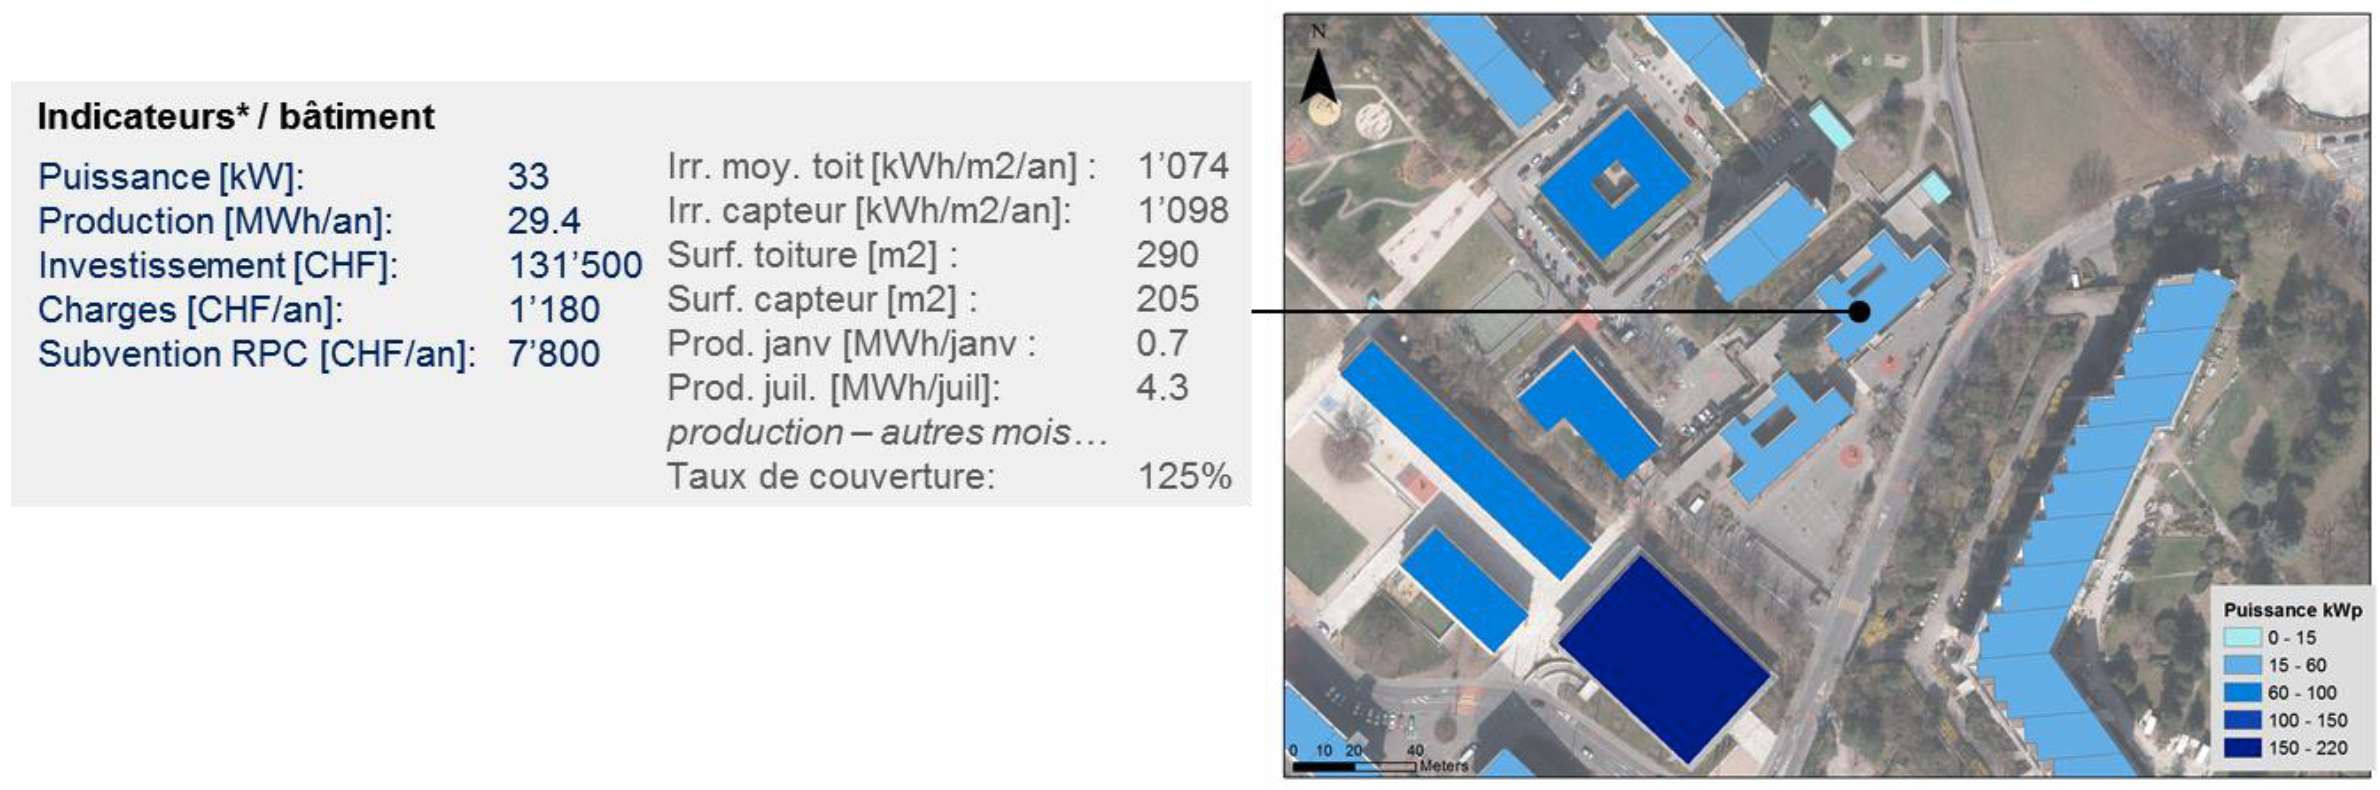
\includegraphics[width=1\linewidth]{02-main//figures/ch2/cadastre_solaire_2014.png}
    \caption{Image d'exemple avec une partie des informations disponibles par bâtiment \cite{desthieux_etude_2014}.}
    \label{fig:cadastre_solaire_2014}
\end{figure}

\par{En 2016, le cadastre a été mis à jour \cite{desthieux_solar_2018}. Les principales nouveautés sont :
\begin{itemize}
    \item L'utilisation des données \gls{lidar} de 2013 \cite{sitg_nuages_2013}
    \item L'amélioration des algorithmes de calcul du potentiel solaire
    \item Utilisation d'un cluster (24 machines) pour réaliser les calculs (environ 900h)
\end{itemize}}

\par{Dès 2018, plusieurs mises à jour \cite{desthieux_solar_2018} sont effectuées. Les principales nouveautés sont :
\begin{itemize}
    \item Prise en compte des toitures et des façades des bâtiments pour l'évaluation du potentiel solaire
    \item Amélioration des algorithmes de calcul du modèle de ciel
    \item Réécriture du code Matlab en Java
    \item Utilisation du cloud CTI IceBOUND
    \item Expansion du cadastre solaire au Grand Genève (canton de Genève, district de Nyon, et pôle métropolitain du Genevois Français)
\end{itemize}}

\par{En 2020, l'article \cite{stendardo_gpu-enabled_2020} de \citeauthor{stendardo_gpu-enabled_2020} aborde la question de l'optimisation des calculs pour le cadastre du Grand Genève. Les auteurs proposent l'utilisation des \acrshort{gpu} pour réduire considérablement les temps de traitement. Cette amélioration répond à un défi croissant : chaque nouvelle version du cadastre intègre davantage de données et requiert des calculs plus précis, ce qui allonge inévitablement les temps d'exécution. L'optimisation du code devient donc un aspect fondamental pour la viabilité du projet.}
\begin{figure}[H]
    \centering
    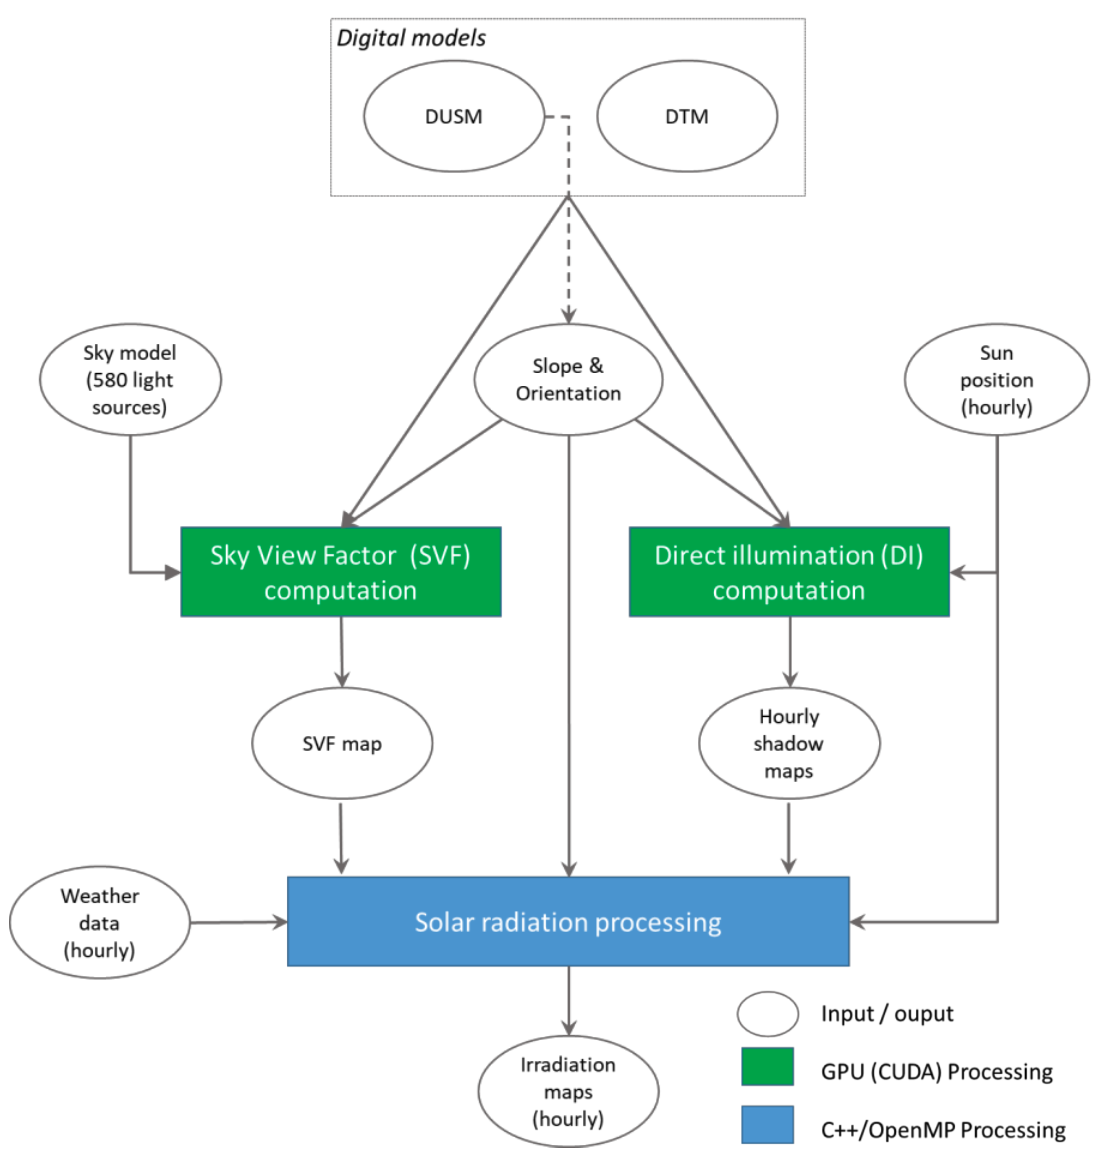
\includegraphics[width=1\linewidth]{02-main//figures/ch2/cadastre_solaire_gpu.png}
    \caption{Schéma pour le calcul d'une tuile \cite{stendardo_gpu-enabled_2020}}
    \label{fig:cadastre_solaire_gpu}
\end{figure}
\par{La Figure \ref{fig:cadastre_solaire_gpu} montre comment le traitement a été repensé pour chaque tuile de 3 x 3 km. Les parties du code Java qui pouvaient être massivement parallélisées ont été réécrites en CUDA \cite{nvidia_cuda_nodate}, ce qui permet de tirer parti des \acrshort{gpu} au lieu de s'appuyer uniquement sur les \acrshort{cpu}. Les autres parties critiques du code ont été optimisées en C++ \cite{noauthor_c_2025}. On peut voir sur la Figure \ref{fig:cadastre_solaire_gpu_evolution_temps} que cette approche a permis de réduire considérablement le temps de traitement par tuile.}

\begin{figure}[H]
    \centering
    \begin{tikzpicture}[scale=1.2]
        % Axes
        \draw[->] (0,0) -- (7,0) node[right] {Année};
        \draw[->] (0,0) -- (0,5) node[above] {Heures};
        
        % Graduations - en commençant par 1 au lieu de 0
        \foreach \y in {1,2,3,4}
            \draw (0.1,\y) -- (-0.1,\y) node[left] {\y0};
        
        % Ajouter le 0 séparément
        \draw (0.1,0) -- (-0.1,0) node[left] {0};
        
        % Années
        \foreach \x/\year in {1/2011, 3.5/2016, 6/2020}
            \draw (\x,-0.1) -- (\x,0.1) node[below=5pt] {\year};
        
        % Données
        \draw[blue, ultra thick] (1,4) -- (3.5,1.6) -- (6,0.2);
        
        % Points
        \filldraw[blue] (1,4) circle (3pt) node[above right] {40h};
        \filldraw[blue] (3.5,1.6) circle (3pt) node[above right] {16h};
        \filldraw[blue] (6,0.2) circle (3pt) node[above right] {2h};
        
        % Annotations
        \node[align=center, font=\small, below] at (1,0) {\\\\Une\\machine};
        \node[align=center, font=\small, below] at (3.5,0) {\\\\Cluster\\24 machines};
        \node[align=center, font=\small, below] at (6,0) {\\\\Une machine\\avec 2 GPU};
    \end{tikzpicture}
    \caption{Évolution des temps de calcul par tuile pour le cadastre solaire (2011-2020).}
    \label{fig:cadastre_solaire_gpu_evolution_temps}
\end{figure}

\subsubsection{Données}
\par{Le cadastre genevois et du \gls{grandgeneve} \cite{desthieux_cadastre_nodate} utilisent plusieurs sources de données. Pour la région de Genève, \acrshort{sitg} a mis à disposition les données \gls{lidar} relevées les années:}
\begin{itemize}
    \item 2009 \cite{sitg_nuages_2009} avec une densité de 5 points au mètre carré. La précision altimétrique est de +/- 20 cm sur surface dure et la précision planimétrique est estimée à 30 cm environ.
    \item 2013 \cite{sitg_nuages_2013} avec une densité de 15 points au mètre carré. La précision altimétrique est de +/- 10 cm sur surface dure et la précision planimétrique est estimée à 20 cm environ.
    \item 2017 \cite{sitg_nuages_2017} avec une densité de 25 points au mètre carré. La précision altimétrique est de +/- 10 cm sur surface dure et la précision planimétrique est estimée à 20 cm environ.
\end{itemize}
\par{En ce qui concerne la région de Nyon, les données \gls{lidar} relevées en 2019 \cite{etat_de_vaud_lidar_nodate} et finalement, pour la France, les données \gls{lidar} relevées en 2014 \cite{ign_ign_nodate} par le \acrshort{ign}.}
\par{Les données vectorielles proviennent des mêmes fournisseurs de données et ne sont pas spécifiées dans les articles. Les données météo proviennent de Météonorm.}


\subsubsection{Méthodologie}

\par{La méthodologie \cite{desthieux_solar_2018} pour la création du cadastre suit les étapes suivantes :}
\begin{itemize}
    \item Collecte des données
    \item Construction du modèle 3D
    \item Calcul des ombrages
    \item Calcul de l'irradiation solaire en chaque point des toits et façades
    \item Calcul des indicateurs et visualisation des résultats
\end{itemize}

\par{La Figure \ref{fig:cadastre_solaire_methodologie} résume ces points.}
\begin{figure}[H]
    \centering
    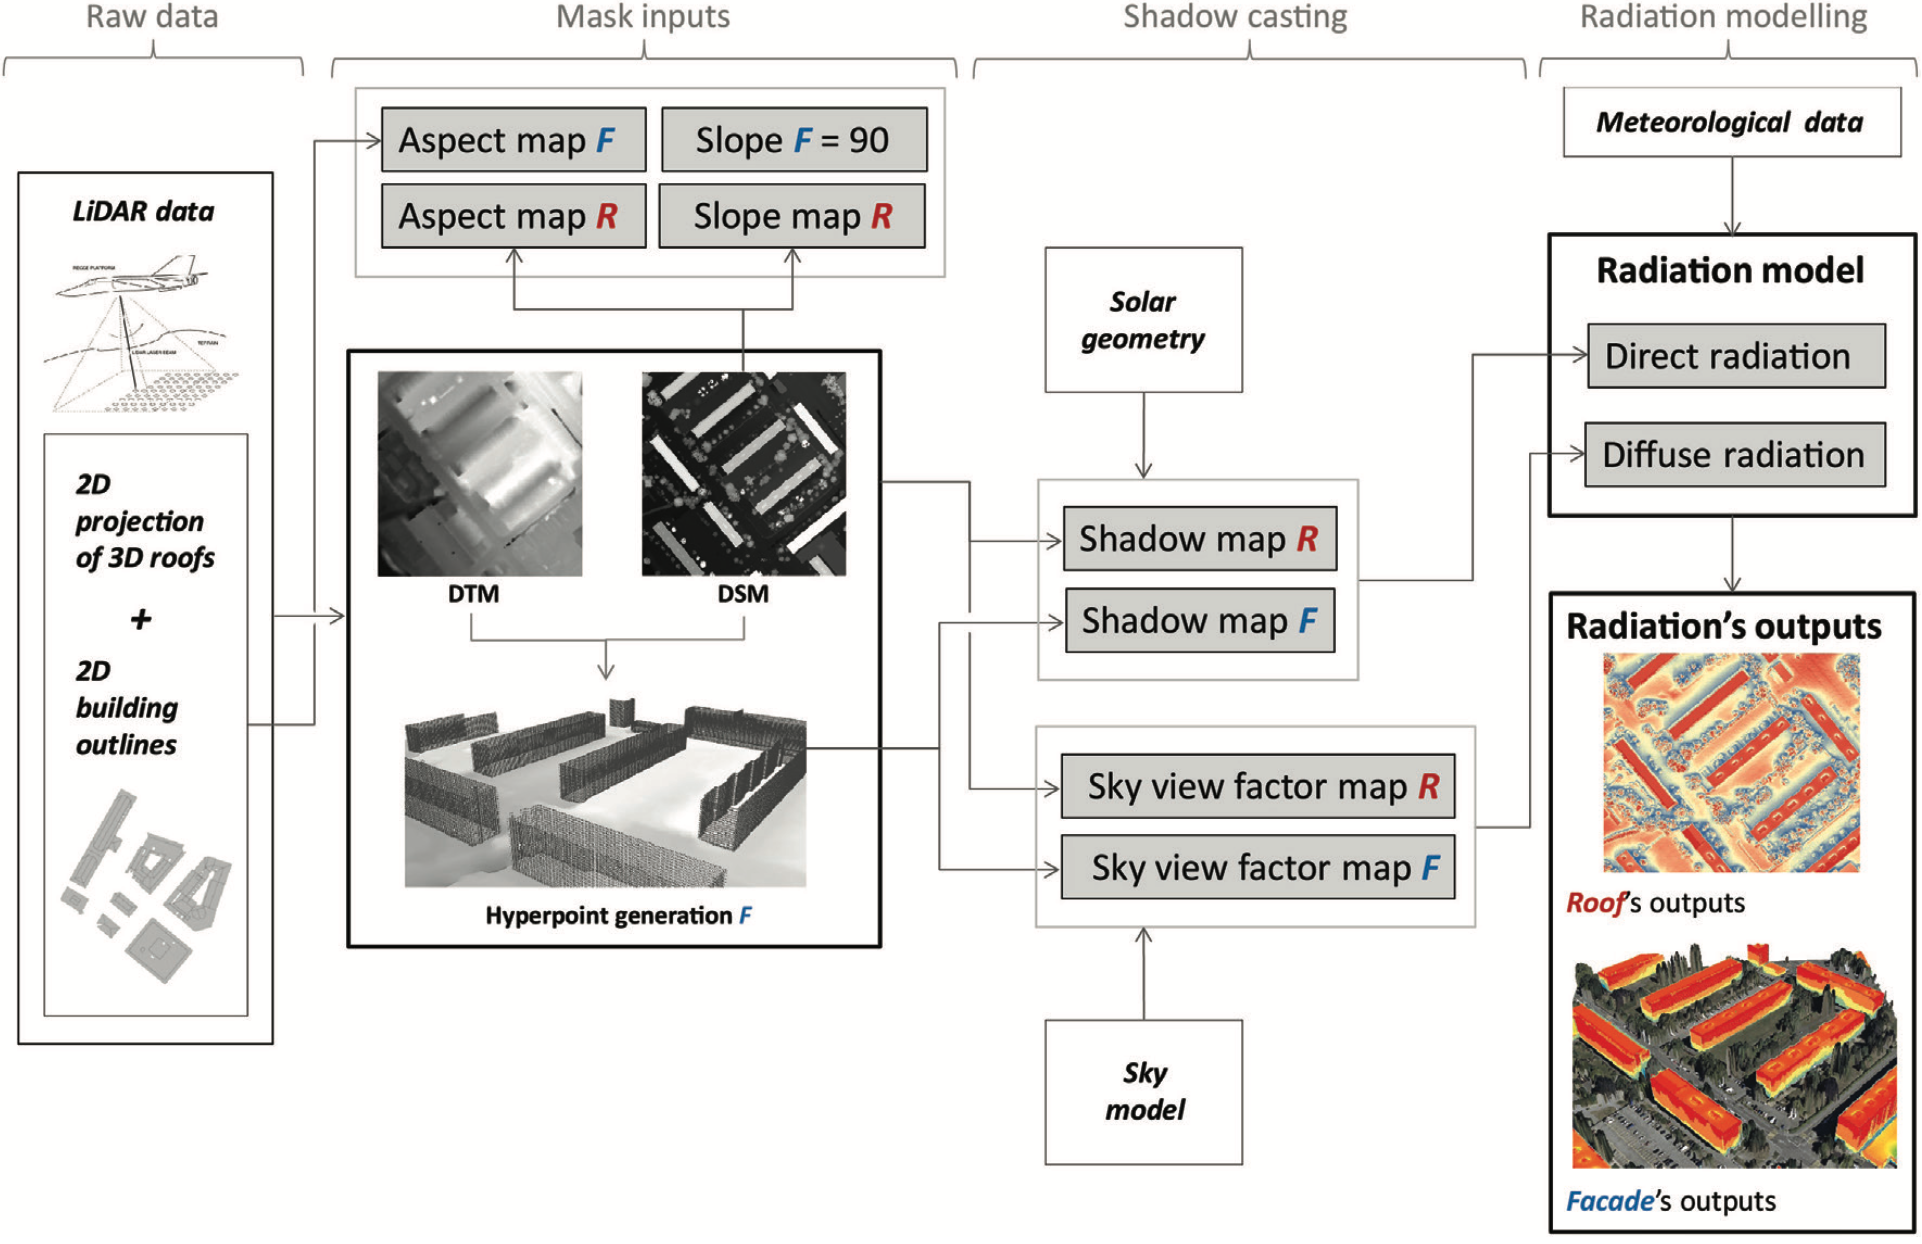
\includegraphics[width=1\linewidth]{02-main//figures/ch2/cadastre_solaire_methodologie.png}
    \caption{Méthodologie utilisée pour la création du cadastre solaire \cite{desthieux_solar_2018}}
    \label{fig:cadastre_solaire_methodologie}
\end{figure}

\paragraph{Collecte des données}
\par{La première étape est d'obtenir les données nécessaires ("Raw data" sur la Figure \ref{fig:cadastre_solaire_methodologie}). À partir des données \gls{lidar}, on construit deux modèles 3D de la ville : un modèle numérique de surface (\acrshort{mns} ou en anglais \acrshort{dsm}) qui représente la surface supérieure des bâtiments et de la végétation, et un modèle numérique de terrain (\acrshort{mnt} ou en anglais \acrshort{dtm}) qui représente le sol nu sans les bâtiments.}
\par{Les contours et empreintes des toits et bâtiments  sont aussi récupérés à partir de données cadastrales existantes, en 2D et 3D. Ils serviront à délimiter précisément les toits et façades.}

\paragraph{Construction du modèle 3D détaillé}
\par{La deuxième étape consiste à construire un modèle 3D détaillé de la ville ("mask inputs" sur la Figure \ref{fig:cadastre_solaire_methodologie}), qui servira de base aux calculs d'ensoleillement. Ce modèle est créé à partir des données récoltées à l'étape précédente.}
\par{Tout d'abord, le modèle numérique de surface (DSM) et le modèle numérique de terrain (DTM) sont transformés en images 3D appelées "rasters". Imaginez une grande grille recouvrant toute la ville, où chaque case de la grille (appelée "pixel") contient une valeur de hauteur. C'est exactement ce que sont le \acrshort{dsm} et le \acrshort{dtm} : des grandes grilles 3D où la hauteur de chaque point de la ville est enregistrée.}
\par{Ensuite, deux modèles 3D distincts sont créés : un pour les toits et un pour les façades. Pour cela, on combine le \acrshort{dsm} obtenu à partir des données \gls{lidar} avec les données cadastrales qui contiennent les contours des bâtiments. Cela permet d'avoir un modèle 3D, où chaque toit et chaque façade est représenté.}
\par{Pour chaque pixel du modèle 3D des toits, deux informations supplémentaires sont calculées : la pente (c'est-à-dire l'inclinaison) et l'orientation (nord, sud, est, ouest...). Ces deux paramètres sont très importants car ils influencent grandement la quantité d'énergie solaire reçue. Par exemple, un toit plat horizontal recevra plus de soleil qu'un toit très pentu orienté vers le nord.}
\par{Le modèle 3D des façades est un peu plus complexe à créer. En effet, un modèle "raster" comme celui des toits ne permet pas de bien représenter les surfaces verticales. Pour contourner ce problème, des points supplémentaires appelés "hyperpoints" sont ajoutés le long des façades (voir Figure \ref{fig:cadastre_solaire_hyperpoints}). Ils permettent de représenter chaque façade comme une série de points verticaux, sur lesquels on pourra ensuite calculer l'ensoleillement de manière précise.}
\begin{figure}[H]
    \centering
    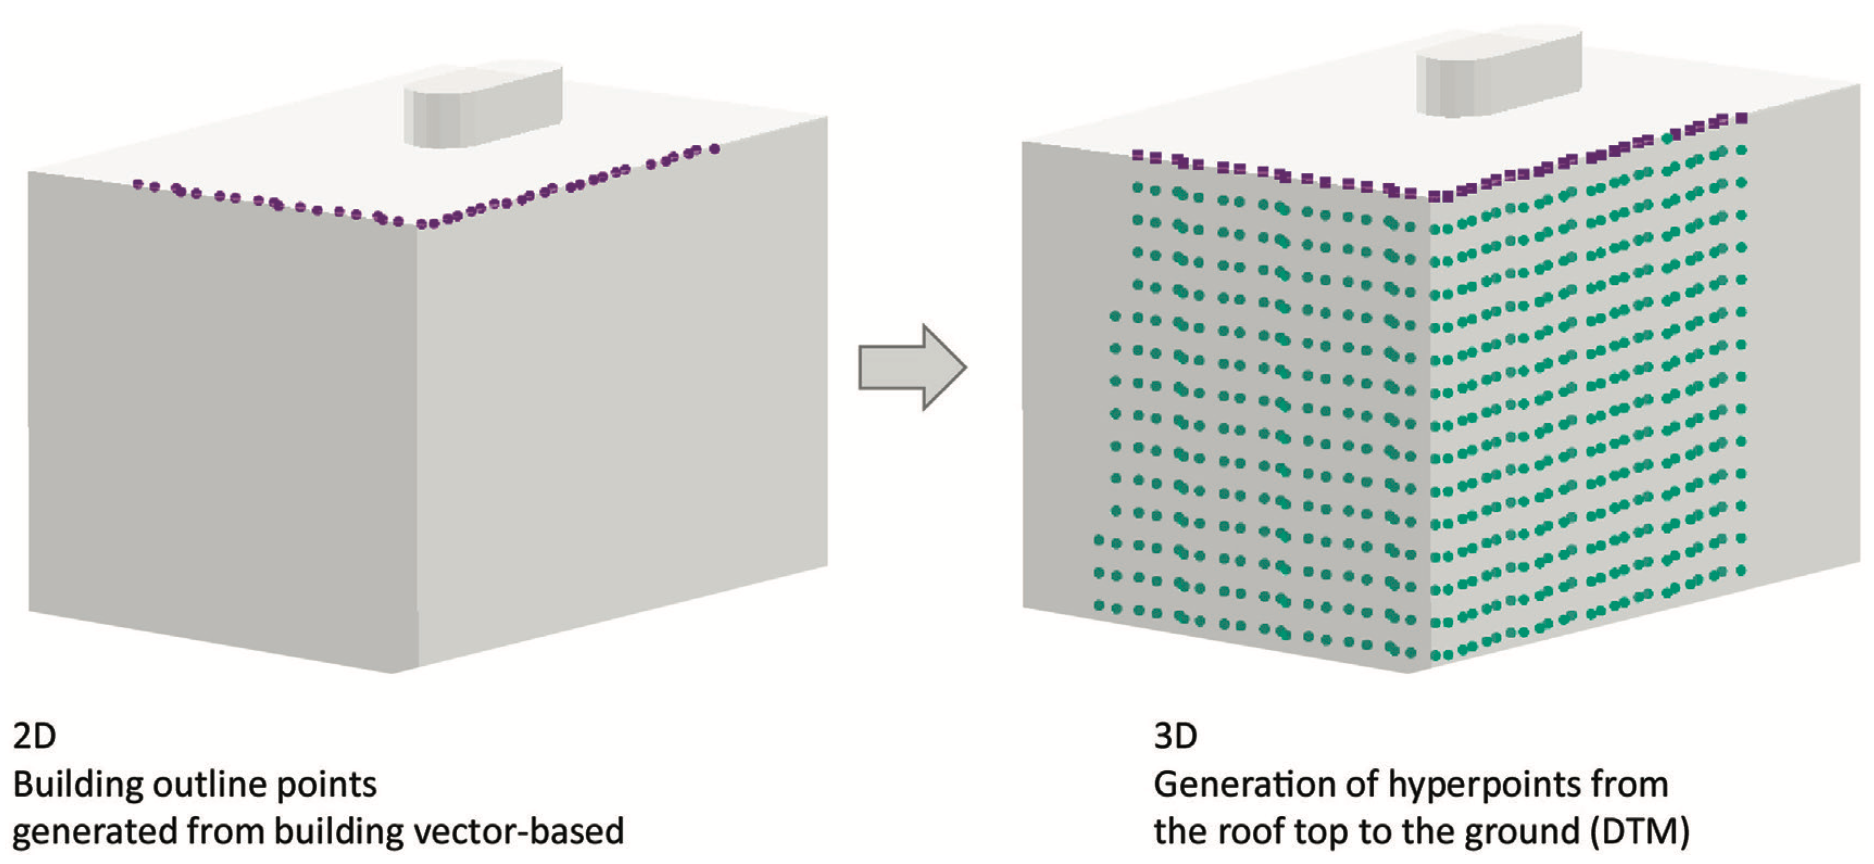
\includegraphics[width=1\linewidth]{02-main//figures/ch2/cadastre_solaire_hyperpoints.png}
    \caption{Méthode de création des hyperpoints sur les façades \cite{desthieux_solar_2018}}
    \label{fig:cadastre_solaire_hyperpoints}
\end{figure}
\par{Finalement, on obtient un jumeau numérique très détaillé de la ville, avec un modèle 3D distinct pour les toits et les façades. Ce jumeau numérique contient toutes les informations nécessaires (hauteur, pente, orientation) pour calculer finement l'ensoleillement en tout point. Les étapes suivantes vont s'appuyer sur ce modèle pour simuler les ombres portées et calculer le potentiel solaire.}

\paragraph{Calcul des zones d'ombre}
\par{La troisième étape consiste à calculer les zones d'ombre sur les toits et les façades des bâtiments (``mask inputs'' sur Figure \ref{fig:cadastre_solaire_methodologie}). Cette étape est cruciale car les zones ombragées ont un potentiel solaire significativement inférieur aux zones bien exposées au soleil.}
\par{Pour réaliser ce calcul, le jumeau numérique 3D de la ville créé précédemment est utilisé comme base. Ce modèle contient toutes les informations nécessaires sur la forme et la hauteur des bâtiments et du relief environnant. Un algorithme de simulation reproduit la course du soleil heure par heure tout au long de l'année, projetant les ombres correspondantes sur le modèle 3D.}
\par{L'ombrage représente l'un des facteurs les plus déterminants pour la performance d'une installation solaire. Pour analyser précisément son impact, trois catégories principales d'ombrages sont identifiées:}
\begin{itemize}
    \item Les ombrages proches: Causés par des éléments situés directement sur le toit comme les cheminées, antennes ou systèmes de ventilation.
    \item Les ombrages lointains: Proviennent du relief naturel (collines, montagnes) ou des grands bâtiments environnants. L'évaluation de leur impact nécessite une étude complète du masque solaire sur l'ensemble de l'année, car leur influence varie considérablement selon les saisons et la position du soleil.
    \item Les ombrages saisonniers: Générés par des éléments variables comme la végétation ou l'accumulation de neige. Ces ombrages évoluent au cours des saisons et nécessitent une gestion adaptative par un entretien régulier et une conception appropriée de l'installation.
\end{itemize}
\begin{figure}[H]
    \centering
    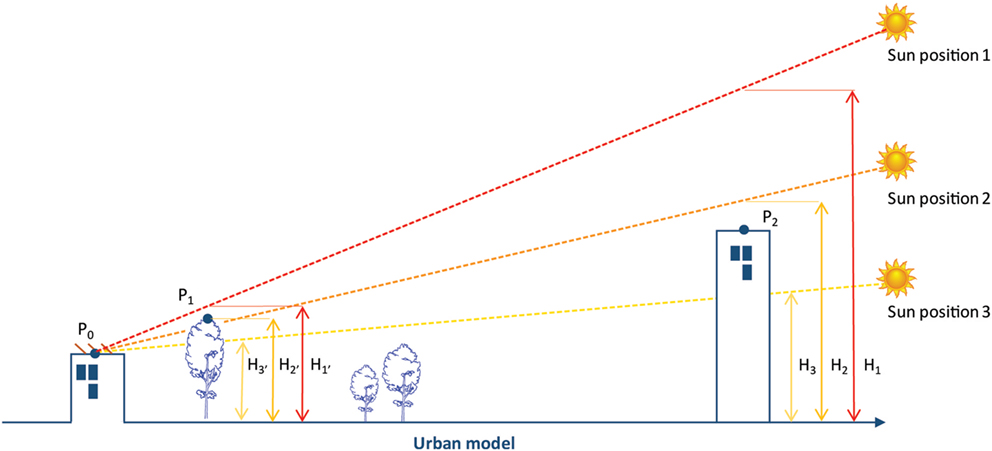
\includegraphics[width=1.00\linewidth]{02-main/figures/ch2/cadastre_solaire_ombrage.jpg}
    \caption{Illustration des différents types d'ombrages \cite{desthieux_solar_2018}}
    \label{fig:cadastre_solaire_ombrage}
\end{figure}
\par{La Figure \ref{fig:cadastre_solaire_ombrage} illustre ces concepts d'ombrage. À la position 1, le soleil n'est obstrué par aucun obstacle, donc le point $P_0$ reçoit un ensoleillement direct. À la position 2, un arbre projette une ombre sur $P_0$, créant un ombrage saisonnier dont l'intensité varie selon le type de végétation et la période de l'année. La position 3 représente une situation typique en milieu urbain où un bâtiment plus élevé projette une ombre sur les structures plus basses. Cette situation peut correspondre à un ombrage proche ou lointain selon la distance et les dimensions du bâtiment obstructif.}
\par{Le résultat de cette analyse produit des "cartes d'ombrage" indiquant, pour chaque heure de la journée, quelles zones des toits et façades sont à l'ombre ou exposées au soleil. Ces cartes constituent une donnée fondamentale pour le calcul final du potentiel solaire.}
\par{En complément de l'ombrage direct, le modèle calcule également le "facteur de vue du ciel" (sky view factor). Ce paramètre mesure la portion de ciel visible depuis un point précis de la ville. Conceptuellement, si une personne se tient à un point donné (représenté en rouge sur la Figure \ref{fig:cadastre_solaire_svf}) et observe le ciel dans toutes les directions, certaines portions seront masquées par les bâtiments, la végétation, ou le relief.}
\begin{figure}[H]
    \centering
    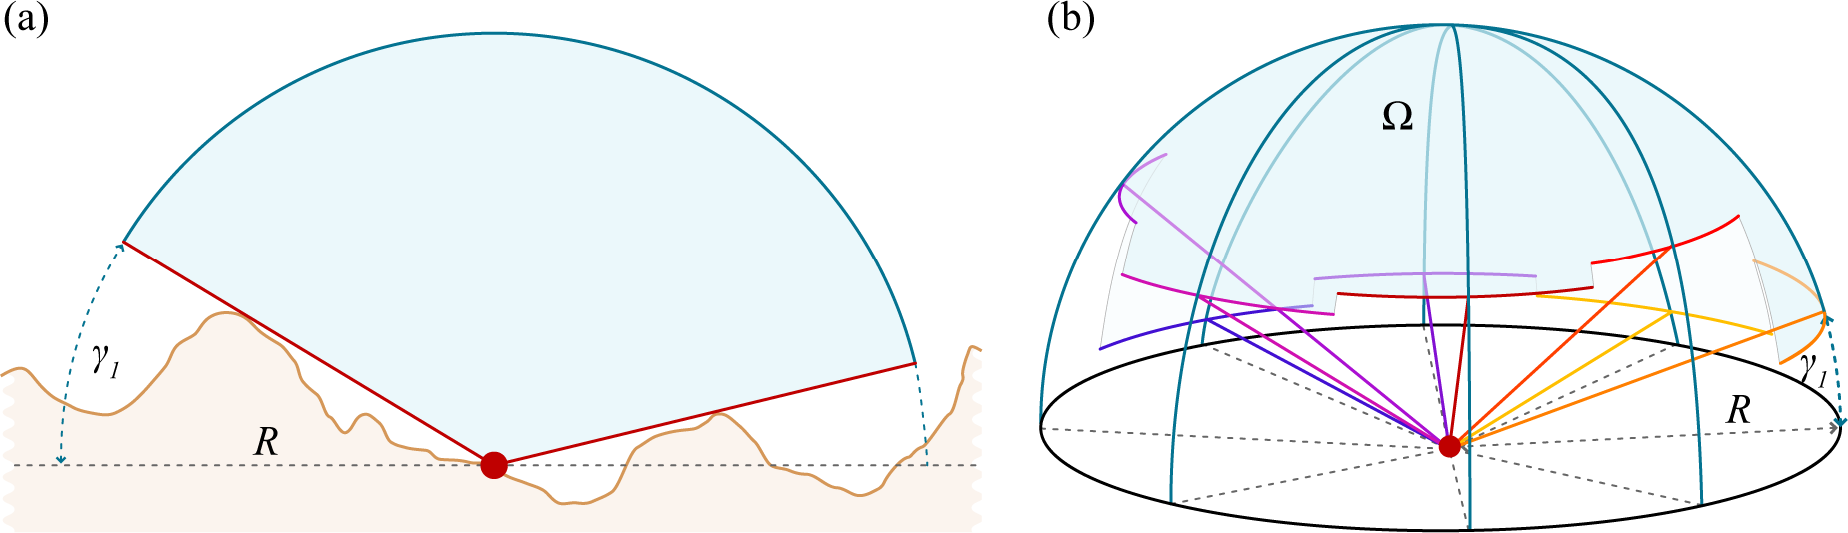
\includegraphics[width=1\linewidth]{02-main/figures/ch2/ch2_cadastre_solaire_svf.png}
    \caption{Le sky view factor (SVF) indique la proportion de ciel visible depuis un point \cite{zaksek_sky-view_2011}}
    \label{fig:cadastre_solaire_svf}
\end{figure}
\par{Le facteur de vue du ciel est exprimé en pourcentage: 100\% correspond à une vue entièrement dégagée (comme au sommet d'une tour ou d'une colline), tandis que 0\% indique un point complètement obstrué (sous un porche ou dans un tunnel). Ce facteur est crucial car il détermine la quantité de lumière naturelle et de rayonnement solaire diffus (indirect) reçue en ce point, en complément du rayonnement direct.}
\par{L'intégration des cartes d'ombrage avec le facteur de vue du ciel fournit une caractérisation complète des conditions d'ensoleillement pour chaque point de la ville. Cette analyse prend en compte à la fois les ombres portées par les obstacles proches et les masques créés par les éléments lointains, constituant ainsi une base solide pour le calcul définitif du potentiel solaire.}

\paragraph{Modélisation du rayonnement solaire}
\par{La quatrième étape consiste à modéliser la quantité d'énergie solaire reçue en chaque point des toits et des façades (``Radiation modelling'' sur Figure \ref{fig:cadastre_solaire_methodologie}), en tenant compte des conditions météorologiques locales et de la position du soleil dans le ciel.}
\par{Pour cela, on récupère tout d'abord des données météorologiques précises pour la zone étudiée :
\begin{itemize}
    \item Le rayonnement solaire global, c'est-à-dire la quantité totale d'énergie solaire reçue sur une surface horizontale.
    \item La part de rayonnement qui arrive en ligne droite du soleil (rayonnement direct).
    \item La part de rayonnement qui arrive de façon indirecte, après avoir été diffusée par les nuages et l'atmosphère (rayonnement diffus).
\end{itemize}}
\par{Ensuite, on utilise des modèles qui reproduisent la position exacte du soleil dans le ciel à chaque heure de la journée et à chaque période de l'année. Cela permet de calculer l'angle avec lequel les rayons du soleil frappent chaque point des toits et des façades.}
\par{En effet, la quantité d'énergie reçue en un point dépend fortement de son orientation (est, sud, ouest...) et de son inclinaison (surface horizontale, verticale ou inclinée). Un point orienté plein sud et incliné à 45° recevra par exemple beaucoup plus d'énergie qu'une façade verticale orientée au nord.}
\par{Les modèles de rayonnement utilisent des équations mathématiques pour calculer précisément la quantité d'énergie directe et diffuse reçue en chaque point, en fonction de tous ces paramètres.}
\par{De plus, ces modèles prennent aussi en compte les effets d'ombrage calculés à l'étape précédente. Ainsi, un point sera considéré comme ne recevant aucune énergie directe s'il est à l'ombre à l'instant considéré.}
\par{Ils intègrent également le "facteur de vue du ciel", qui traduit la portion de ciel visible depuis chaque point. Moins il y a de ciel visible (à cause des bâtiments et du relief alentour), moins il y aura de rayonnement diffus reçu.}
\par{Au final, on obtient une estimation très fine de la quantité d'énergie solaire reçue par chaque mètre carré des toits et façades, heure par heure, tout au long de l'année. Cela permet ensuite de sélectionner les zones les plus intéressantes pour installer des panneaux solaires par exemple.}

\paragraph{Résultats de la simulation}
\par{À la fin de tout ce processus, on obtient des résultats concrets et utilisables sous plusieurs formes. Ces résultats (``Roof outputs'' et ``façade outputs'' sur Figure \ref{fig:cadastre_solaire_methodologie}) sont :
\begin{itemize}
    \item Des cartes de rayonnement solaire pour les toits et façades
    \item Des valeurs d'énergie regroupées par pan de toit, façade, et bâtiment entier
    \item Des indicateurs pratiques comme la production d'énergie possible et la rentabilité économique
\end{itemize}}

\subsubsection{Résultats principaux}
\par{Tous les résultats sont disponibles pour les citoyens et les professionnels sur le géoportail cartographique de \acrshort{sitg} (Figure \ref{fig:cadastre_solaire_couche_vec_sitg}). Ils peuvent être affichés sous forme de couches cartographiques, au même titre que
d'autres données territoriales.}
\begin{figure}[H]
    \centering
    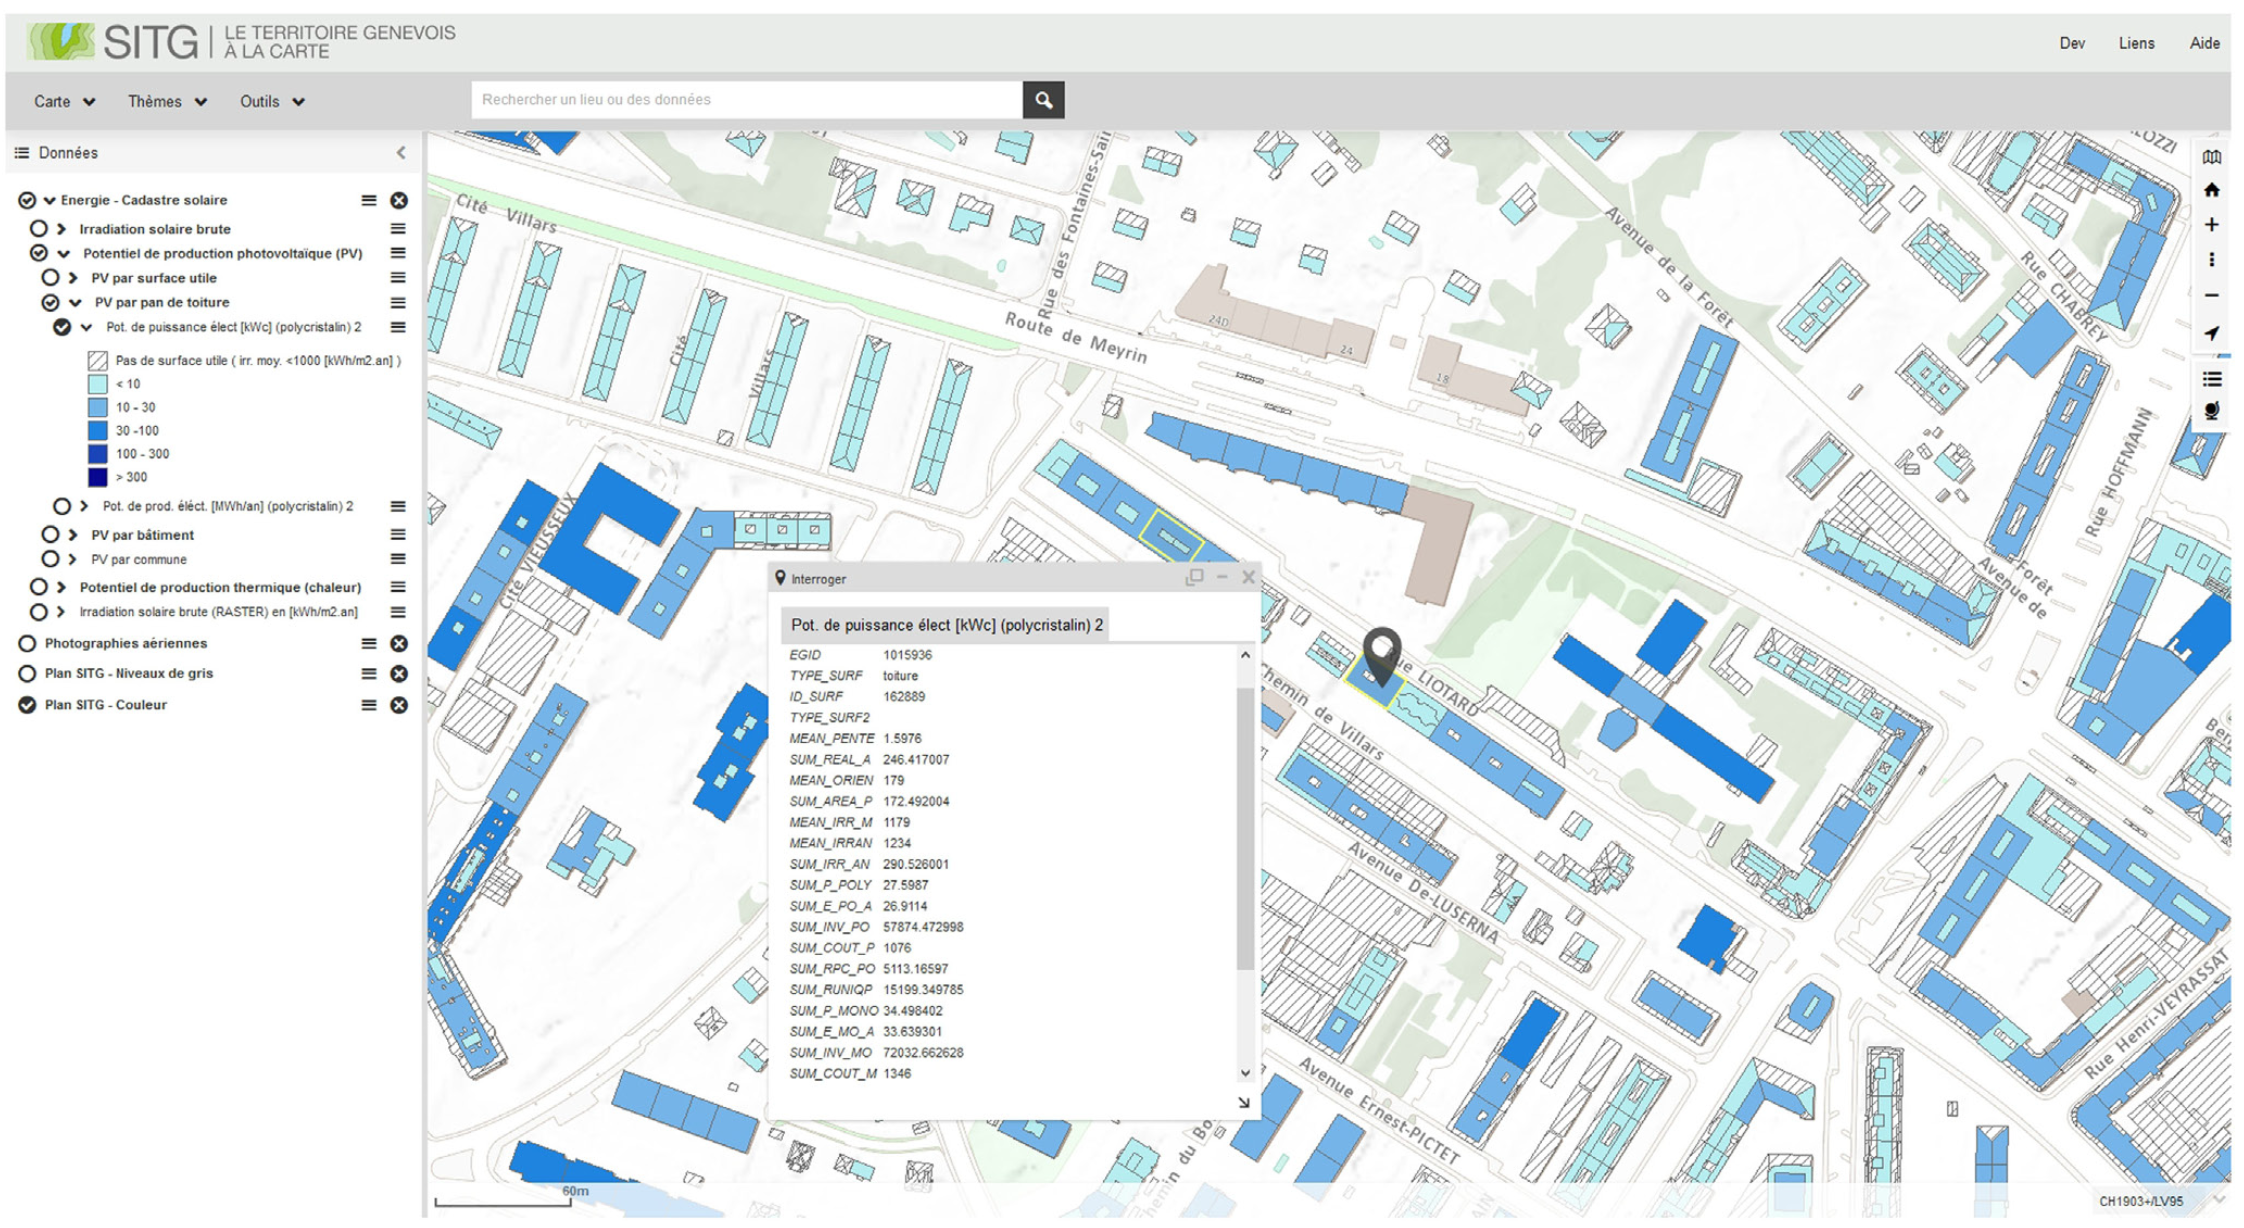
\includegraphics[width=1\linewidth]{02-main//figures/ch2/cadastre_solaire_couche_vec_sitg.png}
    \caption{Visualisation des couches vectorielles sur l'interface \acrshort{sitg} \cite{desthieux_solar_2018}}
    \label{fig:cadastre_solaire_couche_vec_sitg}
\end{figure}
\par{Un site web dédié au cadastre solaire a également été créé (Figure \ref{fig:cadastre_solaire_sitg_labs}). Il permet à chacun de rechercher une adresse et de visualiser très simplement le potentiel solaire du bâtiment correspondant, ainsi que des estimations de production d'énergie et de rentabilité économique.}
\begin{figure}[H]
    \centering
    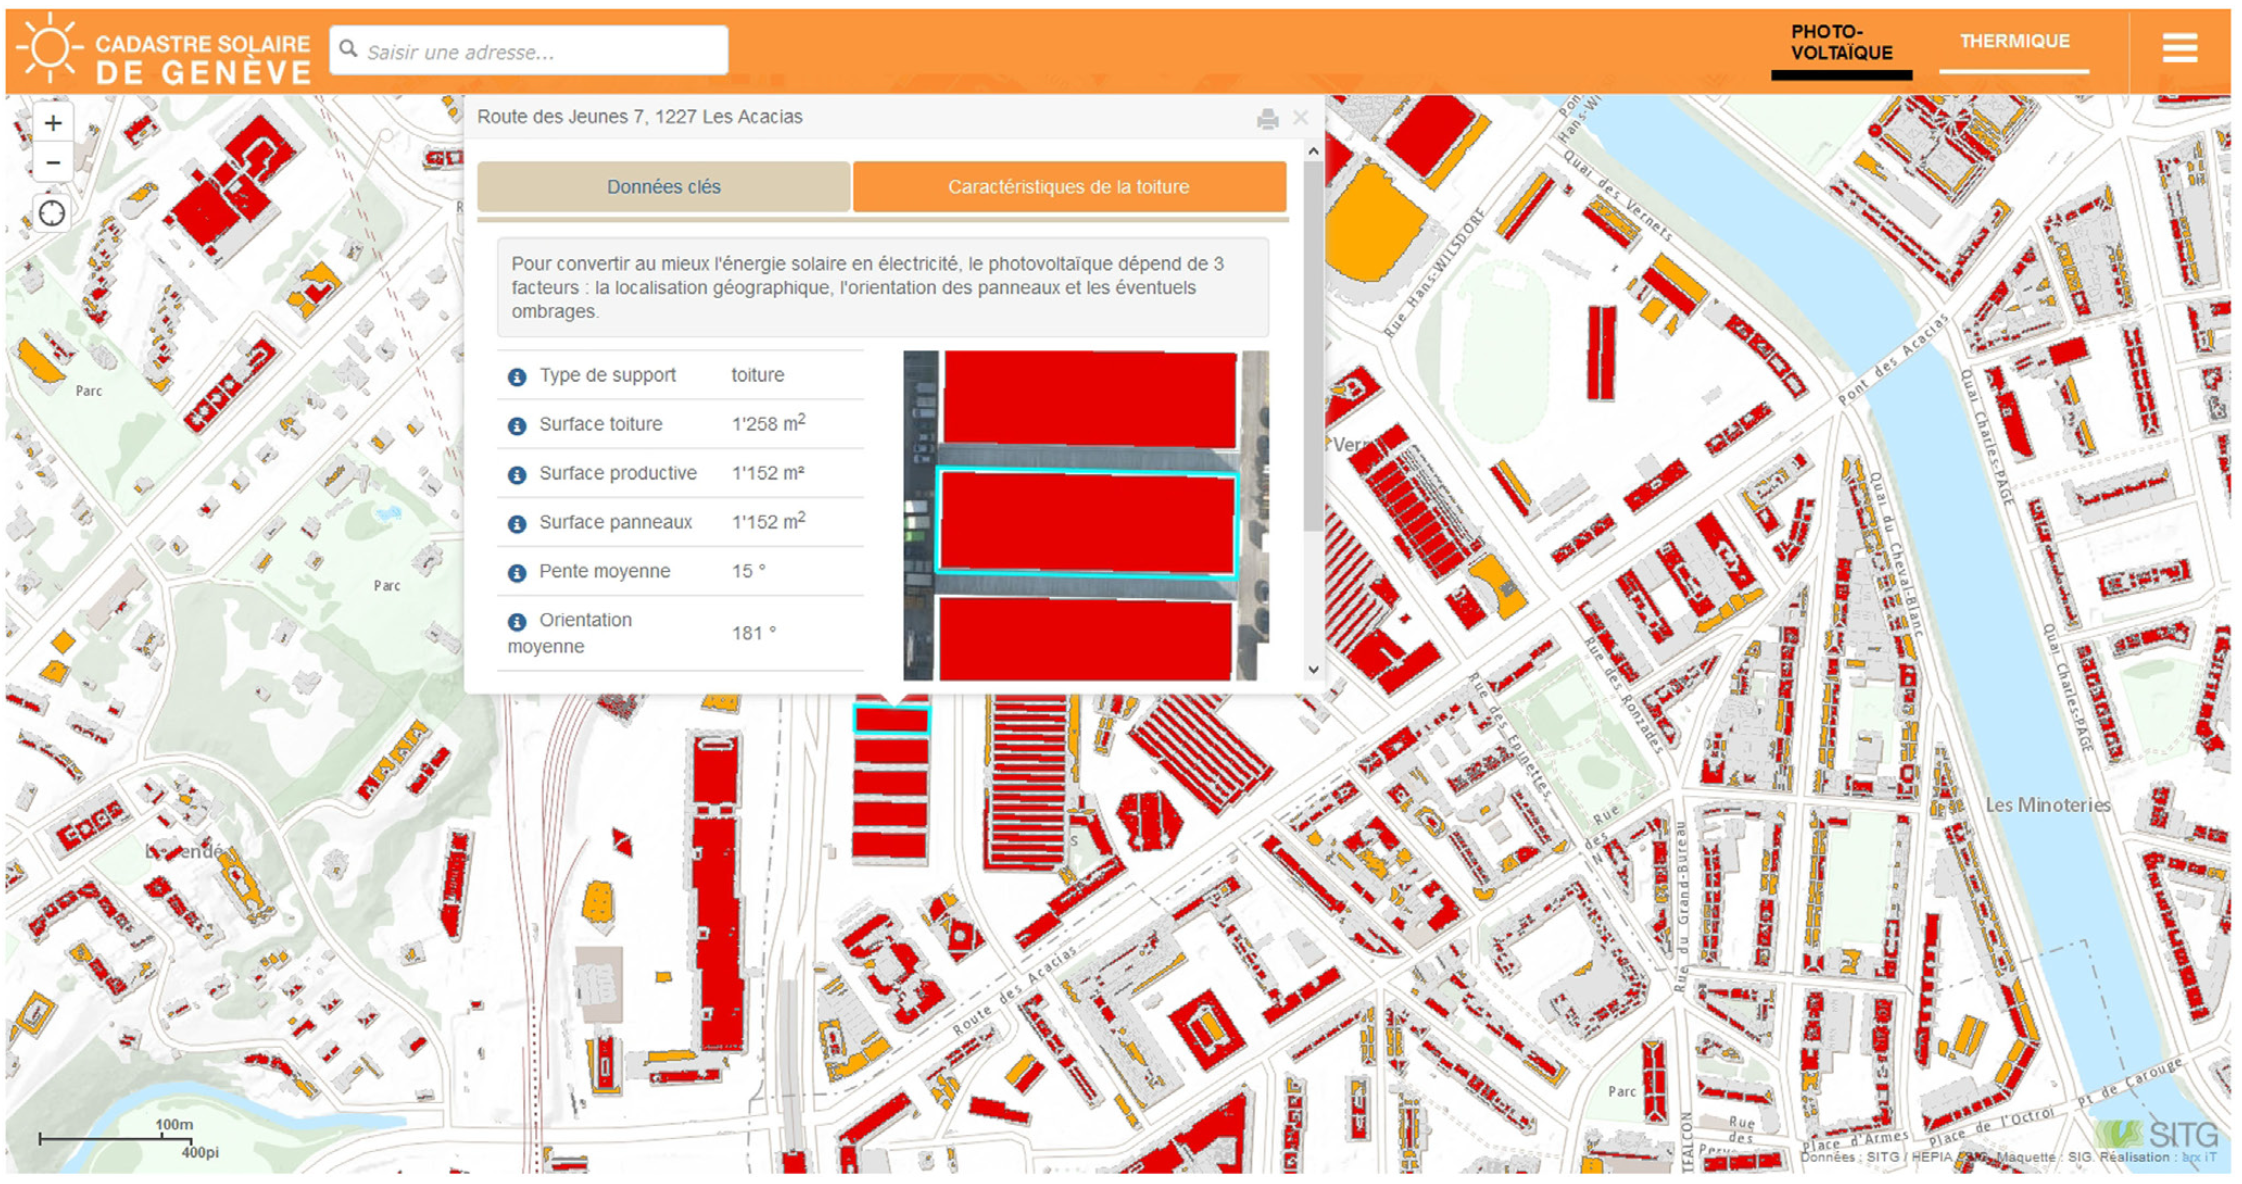
\includegraphics[width=1\linewidth]{02-main//figures/ch2/cadastre_solaire_sitg_labs.png}
    \caption{Interface utilisateur du cadastre solaire destinée au grand public \cite{desthieux_solar_2018}}
    \label{fig:cadastre_solaire_sitg_labs}
\end{figure}
\par{En rendant ces informations facilement accessibles à tous, le cadastre solaire devient un outil précieux pour encourager le développement de l'énergie solaire à Genève, que ce soit pour des projets individuels ou des planifications à grande échelle.}

\subsubsection{Discussion et limites}
\par{L'article de \citeauthor{desthieux_solar_2018} \cite{desthieux_solar_2018} présente une méthodologie complète pour évaluer le potentiel solaire d'une région. Cette approche explore notamment le potentiel des façades, qui constitue un gisement énergétique intéressant mais encore peu exploité. Dans le cadre de ce travail, les façades ne sont pas considérées, leur utilisation étant souvent limitée par des contraintes esthétiques, légales (notamment pour les bâtiments protégés) ou simplement par méconnaissance de leurs avantages. Si certains bâtiments récents intègrent désormais des panneaux solaires en façade, ces installations sont relativement rares.}
\par{Le calculateur a été validée de manière indépendante par l'Université de Genève, ce qui confirme la robustesse de la méthodologie. Un atout majeur réside dans l'utilisation des données relatives aux superstructures \cite{sitg_superstructures_nodate}, qui permet de prendre en compte les ombres projetées par ces éléments sur le reste de la toiture. Cependant, cette couche de données présente certaines limitations, la plupart des toitures comportent des éléments techniques tels que des gaines de ventilation ou des monoblocs qui ne sont pas systématiquement répertoriés dans la couche des superstructures. Ces surfaces pourraient potentiellement être considérées comme utilisables pour l'installation de panneaux solaires, puisqu'elles ne sont pas formellement classées comme superstructures. En définitive, c'est le niveau d'irradiation solaire et la présence ou non d'ombrage qui déterminent véritablement si une surface peut être exploitée efficacement pour la production d'énergie solaire.}

% -----------------------------------------------------------------------------
\subsection{ToitSolaire}

\par{Ce chapitre présente l'application toitsolaire.ch \cite{bfe_wie_nodate} et sa documentation technique \cite{klauser_energie_nodate} qui a été rédigée par l'Office fédéral de l'énergie (\acrshort{ofen}) ainsi que Meteotest \cite{meteotest_wir_2025}.}

\subsubsection{Contexte et objectifs}
\par{L'application toitsolaire.ch, développée par l'\acrshort{ofen}, constitue un cadastre solaire pour l'ensemble du territoire suisse et sert d'instrument d'encouragement pour l'utilisation de l'énergie solaire.}

\par{Ce projet s'inscrit dans la volonté fédérale de favoriser la transition énergétique en fournissant aux propriétaires et aux professionnels un outil permettant d'évaluer rapidement le potentiel solaire des toitures et des façades des bâtiments suisses. L'objectif principal est d'offrir une plateforme en ligne accessible qui présente de manière claire et précise le potentiel d'exploitation de l'énergie solaire pour chaque bâtiment, tant sur les toitures (toitsolaire.ch) que sur les façades (facade-au-soleil.ch).}

\subsubsection{Données}
\par{Le projet s'appuie sur trois types de données principales :}
\begin{itemize}
    \item Données climatiques
    \begin{itemize}
        \item Rayonnement solaire et températures (2011-2020) avec résolution d'environ 2 km, fournies par MétéoSuisse et dérivées de données satellitaires
    \end{itemize}
    \item Données géographiques
    \begin{itemize}
        \item Géométries des bâtiments en 3D (toits et façades) issues du modèle swissBUILDINGS3D 2.0
        \item Modèles numériques de terrain (swissALTI3D, resolution 2m)
        \item Modèles numériques de surface (swissSURFACE3D, résolution 0,5m)
        \item Modèle SRTM (résolution environ 100m)
    \end{itemize}
    \item Données statistiques
        \begin{itemize}
        \item Registre fédéral des bâtiments et des logements (RegBL) pour estimer les besoins en chaleur des bâtiments
        \end{itemize}
    \end{itemize}

\subsubsection{Méthodologie}
\par{Le traitement des données commence par l'analyse des géométries, suivi par le calcul du rayonnement solaire sur les surfaces et se termine par leur classification.}

\paragraph{Traitement des géométries}
\par{Les données 3D des bâtiments sont converties en polygones 2D pour les toits (vue d'oiseau) et polylignes 2D pour les façades. L'orientation, l'inclinaison et la surface de chaque pan de toit sont calculées.}

\paragraph{Calcul du rayonnement solaire}
Trois horizons d'ombrage sont calculés pour chaque surface :
\begin{itemize}
    \item Ombrage lointain (montagnes, collines) dans un rayon de 25 km
    \item Ombrage moyen (voisinage) dans un rayon de 1 km
    \item Ombrage proche (local) dans un rayon de 100 m
\end{itemize}
\par{Le rayonnement solaire sur les surfaces inclinées est calculé à l'aide du modèle anisotrope de Perez, qui tient compte du rayonnement direct, diffus et réfléchi. Les calculs sont effectués heure par heure sur la période 2011-2020.}

\paragraph{Calcul des rendements photovoltaïque et thermique}
\par{Le rendement électrique est calculé en multipliant le rayonnement solaire total par un rendement de module de 19\% et un ratio de performance de 80\%. Pour le solaire thermique, la méthode est plus complexe :}
\begin{itemize}
    \item Estimation des besoins en chaleur du bâtiment à partir des données du RegBL
    \item Dimensionnement d'une installation solaire thermique adaptée à ces besoins
    \item Calcul du rendement thermique à l'aide d'une formule d'approximation validée
    \item Conversion en métriques pratiques (nombre de douches possibles, pourcentage des besoins de chauffage couverts)
\end{itemize}

\paragraph{Classification}
\par{Les surfaces sont classées selon leur potentiel solaire, de "faible" à "excellent", en fonction du rayonnement solaire annuel moyen :}
\begin{itemize}
    \item Pour les toits : < 800, 800-1000, 1000-1200, 1200-1400, > 1400 kWh/m²/an
    \item Pour les façades : < 600, 600-800, 800-1000, 1000-1200, > 1200 kWh/m²/an
\end{itemize}

\subsubsection{Résultats principaux}
\par{Le projet a permis d'analyser environ 10 millions de pans de toit en Suisse, fournissant pour chacun des données géométriques et le potentiel solaire (\acrshort{pv} et solaire thermique) comme données principales.}
\paragraph{Données géométriques} Surface utilisable, orientation et inclinaison.
\paragraph{Potentiel photovoltaïque}
\begin{itemize}
    \item Rayonnement solaire global moyen (kWh/m²/an)
    \item Rayonnement solaire global total (kWh/an)
    \item Production électrique estimée (kWh/an)
\end{itemize}
\paragraph{Potentiel thermique solaire}
\begin{itemize}
    \item Rayonnement solaire global moyen et total
    \item Production thermique estimée
    \item Pourcentage des besoins de chauffage couverts
\end{itemize}
\paragraph{Classification}
\par{Catégorisation de chaque surface selon son aptitude à l'exploitation solaire.}
\paragraph{Paramètres mensuels}
\par{Pour chaque mois, des paramètres permettent de calculer le rayonnement sur surface inclinée à partir du rayonnement horizontal direct et diffus.}
\subsubsection{Discussion et limites}
\par{L'objectif de cet outil est très similaire au cadastre solaire genevois mais pour toute la Suisse. Il a les mêmes limites en ce qui concerne les superstructures des toitures, c'est-à-dire que les éléments de toiture qui ne sont pas renseignés dans la superstructure, seront considérés comme surface apte pour la mise en place de panneaux solaire.}
\par{La modélisation de la météo semble plus sophistiquée que celle du cadastre genevois. L'actualisation des données va dépendre principalement des relevés \gls{lidar} réalisés par swisstopo, mais en principe ceux-ci sont plus fréquents que pour le cadastre solaire genevois}

% -----------------------------------------------------------------------------
% -----------------------------------------------------------------------------
\section{Approche machine learning}

\par{Ce chapitre va permettre d'explorer l'état de l'art en vision par ordinateur appliqué aux données géomatiques.}

% -----------------------------------------------------------------------------
\subsection{Détection des objets présents sur les toitures et identification des espaces libres}
\label{subsec:stdl_analyse}
\vspace{2mm}
\par{Ce sous-chapitre va traiter en détail le projet \cite{herny_detection_2024} réalisé par l'équipe du Swiss Territorial Data Lab (\acrshort{stdl}) pour identifier les objets présents sur les toitures.}

\subsubsection{Résumé}
\par{Les toits libres offrent un potentiel important pour l'installation de nouvelles infrastructures, comme les panneaux solaires et les toits végétalisés, afin de s'adapter au changement climatique. Cependant, il est souvent difficile d'évaluer ce potentiel en raison du manque d'inventaire des objets existants sur les toits.}

\par{Dans le cadre d'un projet \cite{herny_detection_2024} du \acrshort{stdl} avec le Canton de Genève, trois méthodes ont été développées pour identifier automatiquement les surfaces occupées et libres sur les toits. Ces méthodes et leurs résultats sont :}
\begin{itemize}
    \item La classification des pans de toit
    \begin{itemize}
        \item Classification avec un algorithme ``random forrest''
        \item Données : couche vectorielle ``CAD\_BATIMENTS\_HORSOL\_TOIT'' \cite{sitg_toits_nodate}
        \item Precision globale 83\%. Precision d'environ 93\% pour la classe ``potentiellement libre'' et 76\% pour la classe ``occupé''
        \item Demande très peu de ressources informatiques. Plaît aux experts
    \end{itemize}
    \item La segmentation des données \gls{lidar}
    \begin{itemize}
        \item Algorithmes spécifiques pour segmentation nuage de points \gls{lidar} en polygones
        \item Données : données \gls{lidar} du canton de Genève 2019 \cite{sitg_nuages_2019}
        \item F1-score = 0.76 et mIoU = 0.40
        \item Polygones de détection ne sont pas lisses et ne plaisent pas aux experts
    \end{itemize}
    \item La segmentation d'images
    \begin{itemize}
        \item Librairie python ``segment-geospatial'' \cite{wu_samgeo_2023} basé sur segment anything model (SAM) pour détecter et segmenter les objets
        \item Données : Orthophotos du canton de Genève 2019 \cite{sitg_orthophotos_nodate}
        \item F1-score = 0.75 et mIoU = 0.37
        \item Demande beaucoup de ressources informatiques
    \end{itemize}
\end{itemize}

\par{Les résultats des trois méthodes ont été jugés satisfaisants par les experts, 70\% à 95\% des résultats étant considérés comme acceptables. Compte tenu de la qualité des résultats et du temps de calcul, seule la méthode de classification a été retenue pour une application au niveau cantonal.}

\subsubsection{Introduction}

\par{Pour répondre aux défis de la crise climatique et de la transition écologique, il est important que les collectivités locales adaptent leurs politiques d'aménagement du territoire. Une mesure efficace consiste à utiliser les toits pour installer de nouvelles infrastructures, telles que des panneaux solaires ou des toits végétalisés, afin de minimiser l'impact sur l'utilisation des sols.}
\par{Cependant, il est essentiel d'avoir une connaissance précise de la surface disponible et des infrastructures existantes afin de planifier les futurs investissements. Malheureusement, ces informations sont souvent rares et difficiles à tenir à jour, en particulier dans les grandes villes. Cela peut être dû à la complexité des toitures et au nombre croissant d'objets présents. Afin de remédier à cela, l'utilisation d'images aériennes à haute résolution ainsi que des données \gls{lidar} est de plus en plus intéressante. Ces technologies permettent de mieux comprendre le potentiel des toits et de suivre leur évolution.}
\par{Dans un contexte d'urbanisation croissante, il est essentiel de développer des méthodes numériques avancées pour exploiter au mieux les ressources des toits et créer des villes durables.}

\subsubsection{Parties prenantes}

\par{Les principales parties prenantes dans ce projet sont :}
\begin{itemize}
\item Swiss Territorial Data Lab (\acrshort{stdl})
\item Office cantonal de l'énergie du Canton de Genève (\acrshort{ocen})
\item Office cantonal de l'agriculture et de la nature du Canton de Genève (\acrshort{ocan})
\end{itemize}

\par{Le \acrshort{stdl} a pour but de résoudre les problématiques concrètes des administrations publiques en utilisant la science des données appliquée aux géodonnées \cite{stdl_swiss_nodate}.}

Dans le comité de pilotage du \acrshort{stdl} on retrouve :
\begin{itemize}
    \item Office fédéral de topographie swisstopo
    \item Office fédéral de la statistique (OFS)
    \item Conférence des services cantonaux de la géoinformation et du cadastre (CGC)
    \item Ville de Zurich
    \item République et canton de Genève
    \item République et canton de Neuchâtel
    \item Canton des Grisons
\end{itemize}

\par{L'office cantonal de l'énergie du Canton de Genève (\acrshort{ocen}) a pour but de conduire la politique énergétique du canton, notamment en maîtrisant et en réduisant la consommation. Il veille à assurer les conditions d'un approvisionnement durable et fiable en encourageant la production et l'utilisation d'énergies renouvelables et indigènes pour se substituer aux énergies nucléaire et fossile. \cite{etat_de_geneve_office_nodate-1}}

\par{L'Office cantonal de l'agriculture et de la nature (\acrshort{ocan}) promeut la biodiversité et garantit l'intégration de la nature comme de l'agriculture dans l'espace urbain. \cite{etat_de_geneve_office_nodate}}

\subsubsection{Données}

\par{\acrshort{sitg} dispose d'une grande quantité de données géographiques, les données suivantes ont été utilisées dans le cadre de ce projet :}
\begin{itemize}
    \item Nuage de points \gls{lidar} de l'année 2019 \cite{sitg_nuages_2019}
    \item Orthophotos de l'année 2019 \cite{sitg_orthophotos_nodate}
    \item Couche \acrshort{sitg} d'emprise des toitures des bâtiments hors sol ``CAD\_BATIMENTS\_HORSOL\_TOIT'' \cite{sitg_toits_nodate}
\end{itemize}

\paragraph{\gls{lidar}}

\par{Les données \gls{lidar} 2019 \cite{sitg_nuages_2019} de l'État de Genève ont une densité de 25 points au mètre carré. La précision altimétrique est de +/- 10 cm sur surface dure et la précision planimétrique est estimée à 20 cm environ. Le vol de l'avion a été réalisé en mars 2019.}

Chaque point a une classe assignée dont les principales sont :
\begin{itemize}
    \item 1 - Non classifié
    \item 2 – Sol
    \item 3 - Basse végétation (< 50cm)
    \item 5 - Haute végétation (> 50cm)
    \item 6 – Bâtiments
    \item 7 - Points bas ou isolés
    \item 9 – Eau
    \item 13 - Ponts, passerelles
    \item 15 - Sol (points complémentaires)
    \item 16 – Bruit
    \item 19 - Points mesurés hors périmètre de l'acquisition
\end{itemize}

\paragraph{Orthophotos}
\par{Le canton de Genève a réalisé en mai 2019 des images aériennes de haute résolution \cite{sitg_orthophotos_nodate} de tout le canton qui ont ensuite été converties en true orthophotos (XXXXX)}
\todo[inline]{Ajouter ici le lien correct à l'annexe des ortophotos}
\par{Ces orthophotos ont la particularité de ne pas avoir de décalage vis-à-vis d'un modèle numérique du terrain, donc les couches vectorielles devraient s'aligner avec les orthophotos. Chaque pixel représente 5 cm.}

\paragraph{Couche vectorielle d'emprise au sol des toitures}
\par{\acrshort{sitg} dispose d'une couche vectorielle d'emprise des toitures des bâtiments hors sol ``CAD\_BATIMENTS\_HORSOL\_TOIT'' \cite{sitg_toits_nodate}. Cette couche provient de la numérisation 3D des bâtiments. La Figure \ref{fig:stdl_01_couche_vectorielle} représente un exemple de cette couche avec une orthophoto en fond d'image.}
\begin{figure}[H]
    \centering
    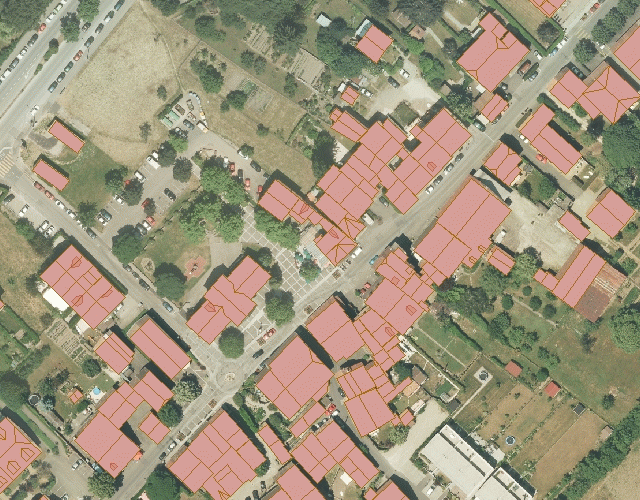
\includegraphics[width=1\linewidth]{02-main//figures/ch2/stdl_01_couche_vectorielle.png}
    \caption{Image d’exemple de la couche vectorielle d’emprise au sol des bâtiments ``CAD\_BATIMENTS\_HORSOL\_TOIT'' \cite{sitg_toits_nodate}}
    \label{fig:stdl_01_couche_vectorielle}
\end{figure}
\par{Cette couche est régulièrement mise à jour. \acrshort{stdl} a utilisé les données de mars 2023 pour son projet. Les superstructures sont des éléments qui dépassent de la toiture tel qu'une cheminée, cage d'ascenseur, lucarne, etc. ne sont pas représentés dans cette couche. Tout ce qui est en dessous de 9 m² ne figure pas dans cette couche.}

\paragraph{Vérité terrain}
\par{La Figure \ref{fig:stdl_02_verite_terrain} représente les bâtiments choisis par \acrshort{stdl} pour la vérité terrain.}
\begin{figure}[H]
    \centering
    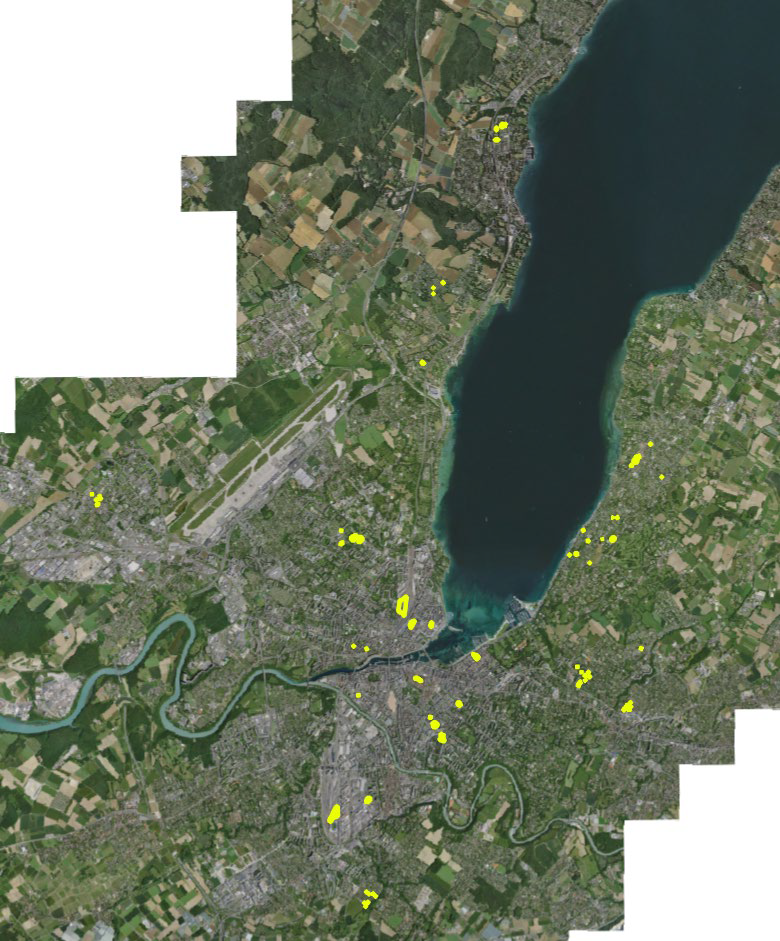
\includegraphics[width=1\linewidth]{02-main//figures/ch2/stdl_02_verite_terrain.png}
    \caption{Bâtiments choisis par STDL pour la vérité terrain dans le Canton de Genève. Images de \acrshort{sitg}}
    \label{fig:stdl_02_verite_terrain}
\end{figure}
\par{Ces bâtiments se distribuent de la manière suivante :}
\begin{itemize}
    \item 7 bâtiments administratifs (toiture plate)
    \item 18 bâtiments industriels (toiture plate)
    \item 97 bâtiments de logement (toiture en pente/plate)
\end{itemize}
\par{Les données ont été labellisées selon les classes suivantes :}
\begin{figure}[H]
    \centering
    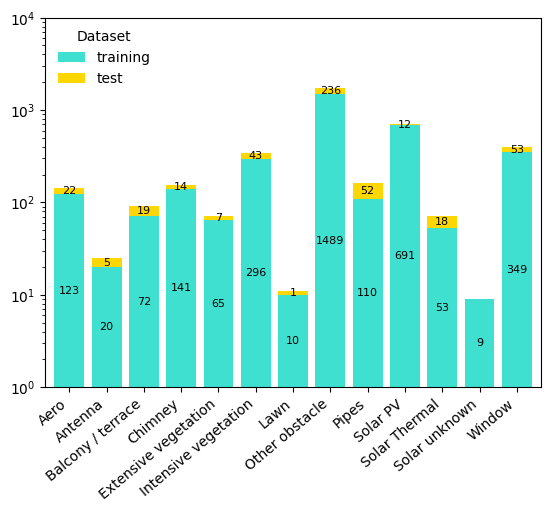
\includegraphics[width=1\linewidth]{02-main//figures/ch2/stdl_03_classes.png}
    \caption{Classes et répartition des datasets}
    \label{fig:stdl_03_classes}
\end{figure}
\par{Chaque méthode utilisée dans ce projet nécessite la création de vérité terrain spécifique.}

\subsubsection{Classification des pans de toits}
\par{Cette méthode consiste à utiliser les données vectorielles de l'emprise des toitures, les labelliser à l'aide des données \gls{lidar} et ensuite appliquer un algorithme random forest (similaire a un arbre de décision).}

\paragraph{Données}
\par{Les données utilisées sont la couche vectorielle de l'emprise des toitures, ainsi que les données \gls{lidar}.}
\par{Comme indiqué au chapitre ``XXXXXX'', la rugosité et l'intensité sont deux informations complémentaires fournies par les nuages de points \gls{lidar}. La rugosité mesure la variation locale de l'altitude des points et reflète la texture de la surface. Une rugosité élevée indique la présence d'obstacles. L'intensité mesure la quantité d'énergie réfléchie par la surface et dépend des propriétés de réflectance des matériaux. Elle varie selon le type de surface et peut aider à distinguer différents matériaux.}
\todo[inline]{Ajouter ici le lien correct aux annexes}
\par{Pour constituer le dataset (vérité terrain), \acrshort{stdl} a annoté la couche vectorielle de l'emprise des toitures avec l'aide des données \gls{lidar}. Les 3 classes résultantes sont :}
\begin{itemize}
    \item Occupé : pas de surface disponible
    \item Possiblement libre : probablement libre
    \item Non défini : le nuage de point \gls{lidar} n'a pas classifié cette zone comme ``bâtiment''
\end{itemize}

\paragraph{Méthodologie}
\par{La méthodologie se décompose en trois étapes principales : la préparation des données \gls{lidar}, la classification par seuils manuels et la classification par forêt aléatoire (random forest).}
\par{La première étape est la préparation des données \gls{lidar} :}
\begin{itemize}
    \item L'intensité du signal \gls{lidar} est interpolée par une méthode de pondération inverse à la distance pour obtenir une valeur continue en chaque point.
    \item Un modèle numérique de terrain (\acrshort{mnt}) est généré à partir des points \gls{lidar} pour représenter la surface du sol.
    \item La rugosité de la surface est calculée à partir du \acrshort{mnt} à une échelle de 1 m pour caractériser les variations locales de hauteur.
    \item Des statistiques zonales (moyenne, médiane, écart-type, etc.) sont calculées pour l'intensité et la rugosité sur chaque pan de toit.
\end{itemize}
\par{La deuxième étape est la classification par seuils manuels :}
\begin{itemize}
    \item Les pans de toit de moins de 2 m² sont automatiquement classés comme "occupés" car trop petits pour des installations.
    \item Les pans avec moins de 25\% de points classés comme "bâtiment" (données \gls{lidar}) sont classés en "non défini" par manque d'information.
    \item Pour les autres pans
    \begin{itemize}
        \item Des seuils sont fixés empiriquement sur 4 variables :
        \begin{itemize}
            \item La marge d'erreur et l'écart-type de l'intensité
            \item La rugosité médiane
            \item Le pourcentage de recouvrement avec des pixels non classés comme "bâtiment" (données \gls{lidar})
        \end{itemize}
        \item Si un pan dépasse le seuil pour au moins une variable, il est classé comme "occupé", sinon il est "potentiellement libre".
    \end{itemize}
    \item Cette classification est validée manuellement par des experts sur un échantillon de 650 pans de toit.
\end{itemize}
\par{La troisième étape est la classification par random forrest (RF)}
\begin{itemize}
    \item Deux forêts aléatoires sont entraînées, une pour chaque office (\acrshort{ocen} et \acrshort{ocan}), en utilisant les seuils validés comme référence.
    \item Les données sont divisées en 80\% pour l'entraînement et 20\% pour le test.
    \item 14 variables sont utilisées pour construire les arbres de décision, dont les statistiques zonales d'intensité et de rugosité.
    \item L'importance relative de chaque variable dans la classification est calculée.
    \item Les forêts sont évaluées sur l'échantillon test pour mesurer leur performance.
\end{itemize}

\paragraph{Résultats}
\par{Les résultats obtenus sont détaillés dans le Tableau \ref{tab:stdl_01_resultats_classification} :}
\begin{table}[h]
    \centering
    \begin{tabular}{|l|c|c|c||c|c|c|}
    \hline
    \multirow{2}{*}{} & \multicolumn{3}{c||}{Manual threshold classification} & \multicolumn{3}{c|}{RF classification} \\
    \cline{2-7}
    & Global & Occupied & Potentially free & Global & Occupied & Potentially free \\
    \hline
    OCAN & 79\% & 70\% & 91\% & 86\% & 78\% & 96\% \\
    OCEN & 77\% & 72\% & 82\% & 83\% & 74\% & 91\% \\
    \hline
    \end{tabular}
    \caption{Résultats obtenus par les deux algorithmes de classification}
    \label{tab:stdl_01_resultats_classification}
\end{table}
\par{La classification avec RF est plus performante que les seuils manuels, avec des taux de satisfaction augmentant de 7 et 6 points pour \acrshort{ocan} et \acrshort{ocen} respectivement.}

\par{La Figure \ref{fig:stdl_04_rf_resultats} présente un aperçu des résultats obtenus :}
\begin{figure}[H]
    \centering
    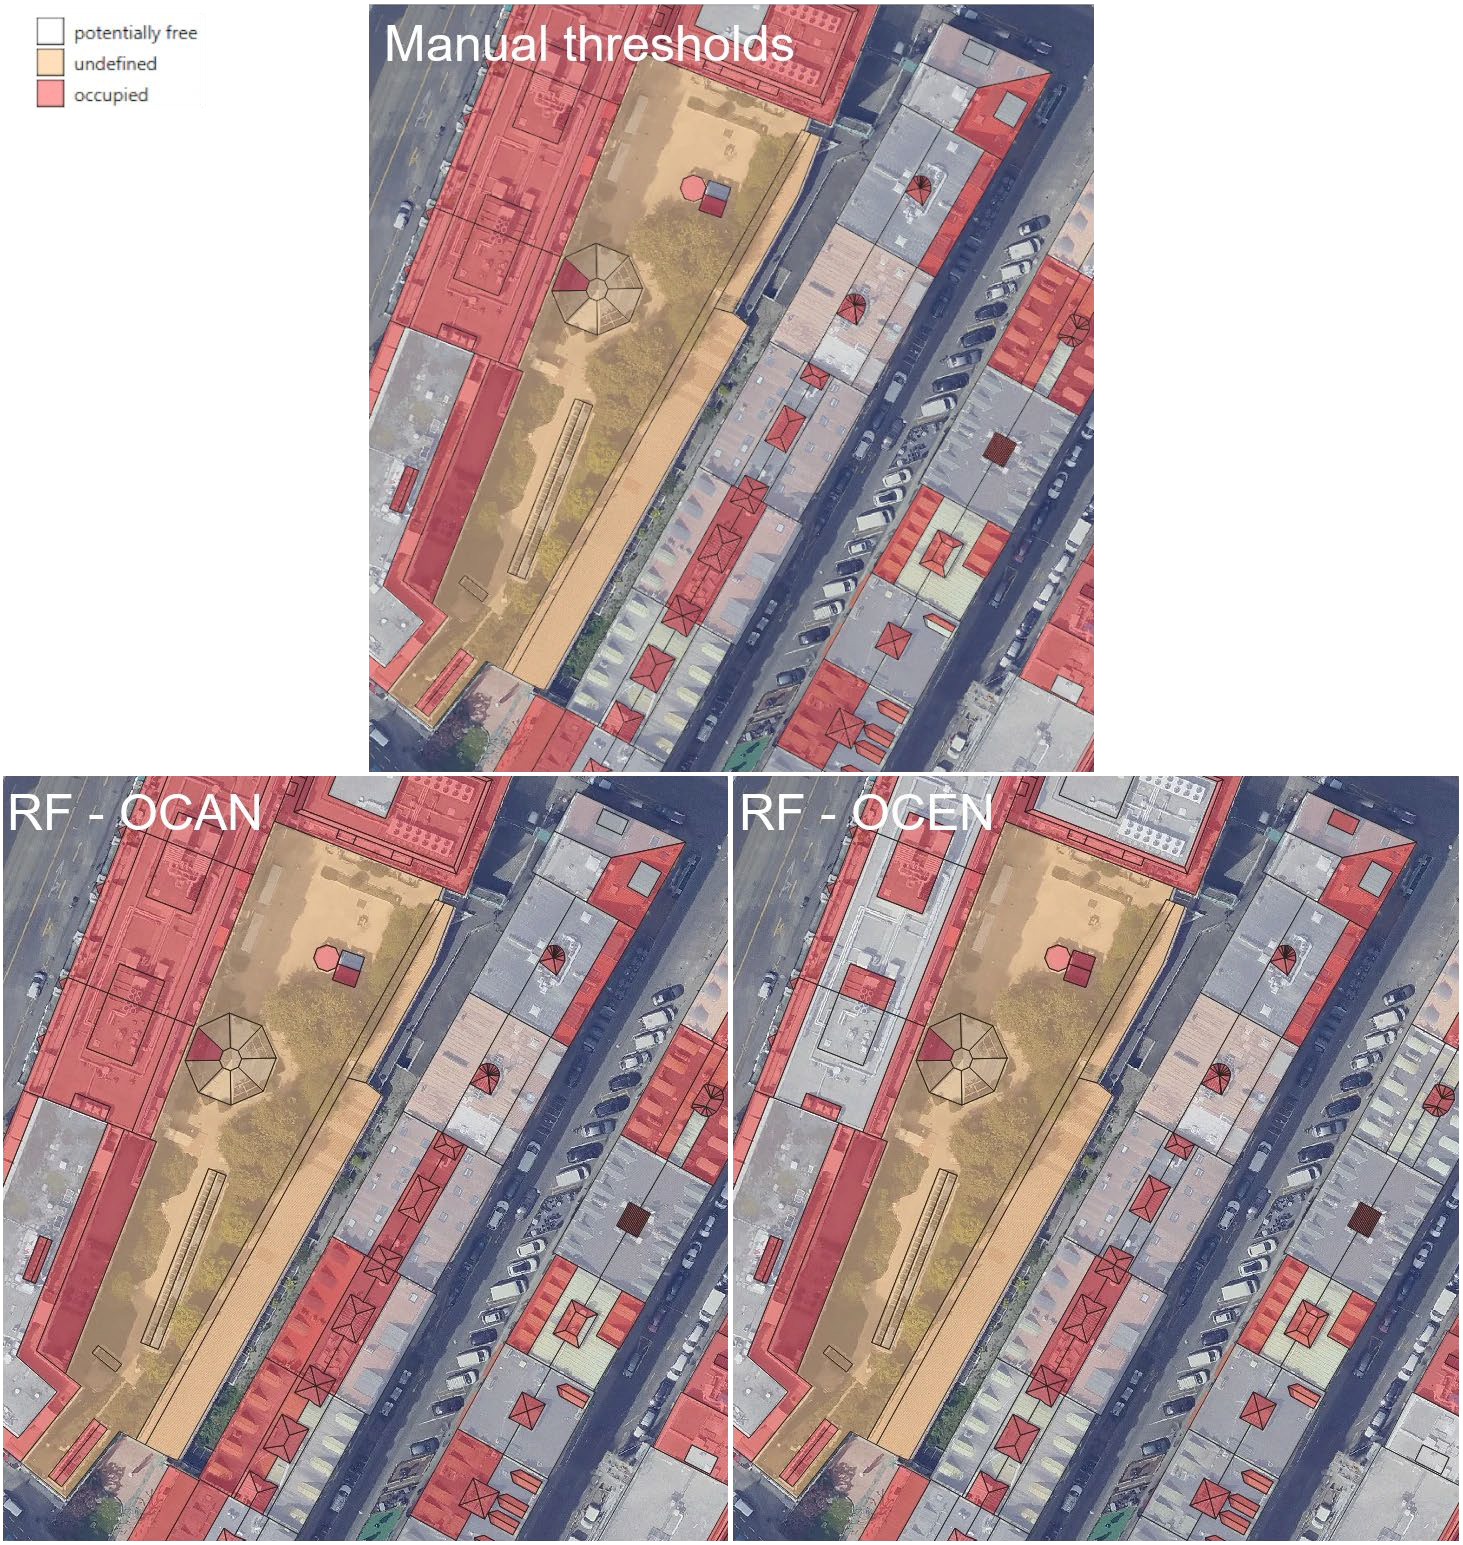
\includegraphics[width=1\linewidth]{02-main//figures/ch2/stdl_04_rf_resultats.png}
    \caption{Comparatif des différents algorithmes de classification \cite{herny_detection_2024}}
    \label{fig:stdl_04_rf_resultats}
\end{figure}
\par{Dans la Figure \ref{fig:stdl_04_rf_resultats} on observe les différents critères par office, l'\acrshort{ocen} semble classifier plus de surfaces comme ``possiblement libre'' (blanc) que l'\acrshort{ocan}. Une matrice de confiance aurait permis de mieux évaluer les résultats.}

\paragraph{Discussion des résultats (\acrshort{stdl})}
\par{Dans son rapport \acrshort{stdl} fait une analyse des résultats obtenus dans lequel ils traitent les points suivants :}
\begin{itemize}
    \item Comparaison des deux méthodes de classification
    \item Classification des petits pans de toit
    \item Différences entre les deux random forrest
    \item Pertinence de la méthodologie
\end{itemize}
\par{Le premier point soulevé est une comparaison de la classification par seuils et celle avec la random forrest :}
\begin{itemize}
    \item Les deux méthodes donnent des résultats satisfaisants, mais la forêt aléatoire est plus performante.
    \item La forêt aléatoire utilise 14 variables, contre seulement 4 pour les seuils manuels.
    \item Le choix des variables pour les seuils manuels était pertinent mais incomplet.
    \item Les seuils manuels sont simples à mettre en place mais nécessitent des tests manuels fastidieux.
    \item La forêt aléatoire est automatisée mais a besoin d'une vérité terrain.
\end{itemize}
\par{Le deuxième point est la classification des petits pans de toit :}
\begin{itemize}
    \item Avec les seuils manuels, les petits pans sont souvent classés comme "occupés" à cause de leur rugosité médiane élevée.
    \item La rugosité des petits pans est plus influencée par leur environnement à cause de l'échelle de calcul (1 m).
    \item La rugosité minimale, importante dans la forêt aléatoire, dépend fortement de la taille du pan.
    \item Bien que potentiellement utilisables, les petits pans dégagés sont difficiles à exploiter et moins prioritaires.
    \item Le fait que l'algorithme les classe souvent comme occupés convient aux experts.
\end{itemize}

\par{Le troisième point traite des raisons des différences entre les deux random forrest (une par office) :}
\begin{itemize}
    \item Les différences de résultats entre les offices (\acrshort{ocan} et \acrshort{ocen}) s'expliquent par leurs besoins distincts.
    \item Pour l'\acrshort{ocan} (végétalisation), une rugosité médiane élevée est tolérée.
    \item Pour l'\acrshort{ocen} (solaire), une grande surface continue et une faible rugosité minimale sont requises.
\end{itemize}

\par{Le quatrième point est la pertinence de la méthodologie utilisée :}
\begin{itemize}
    \item Les surfaces "potentiellement libres" doivent être examinées plus en détail.
    \item Les surfaces "occupées" sont considérées comme inutilisables.
    \item Les experts sont satisfaits des résultats obtenus.
    \item Il est prévu d'appliquer la méthode à plus grande échelle.
    \item La classification n'évalue que l'occupation, sans considérer la pente ou le matériau.
    \item L'intensité \gls{lidar} peut varier entre les acquisitions, affectant potentiellement les résultats.
\end{itemize}

\subsubsection{Segmentation \gls{lidar}}

\paragraph{Données}
\par{Les données utilisées sont des nuages de points \gls{lidar}, qui fournissent une représentation 3D précise des surfaces de toiture. Les toits sont délimités à partir d'une couche vectorielle existante, produite manuellement pour garantir sa qualité. Les points \gls{lidar} sont filtrés pour ne conserver que ceux situés au-dessus de l'altitude minimale de chaque toit.}

\paragraph{Méthodologie}
\par{La méthode proposée vise à détecter automatiquement les objets présents sur les toits, en supposant que chaque pan de toit peut être approximé par un plan et que les obstacles en dépassent. Le processus se déroule en plusieurs étapes :}
\begin{enumerate}
    \item Segmentation des plans de toit dans le nuage de points 3D à l'aide de l'algorithme RANSAC (RANdom SAmple Consensus), qui permet d'identifier les plans dominants.
    \item Application de l'algorithme DBSCAN (Density-Based Spatial Clustering of Applications with Noise) sur les points de chaque plan potentiel pour éliminer le bruit et ne retenir que le plus grand cluster.
    \item Considération des points restants comme des obstacles, regroupés à nouveau avec DBSCAN.
    \item Transformation des clusters de points en polygones concaves à l'aide de l'algorithme ``alpha shape'', en appliquant des seuils sur leur surface projetée pour distinguer les plans des obstacles.
    \item Optimisation des hyperparamètres des algorithmes RANSAC et DBSCAN, ainsi que des seuils de surface, sur un jeu de données d'entraînement, en tenant compte du type de bâtiment et de toit.
    \item Post-traitement des polygones détectés par lissage et fusion pour améliorer leur aspect visuel et créer une partition des surfaces occupées et libres sur chaque toit.
\end{enumerate}

\newpage
\paragraph{Résultats}
\par{Les experts de l'\acrshort{ocen} et l'\acrshort{ocan} n'ont pas apprécié les images résultantes (Figure \ref{fig:stdl_05_exemple_segmentation_lidar}) car ils s'attendaient à des polygones plus semblables aux couches vectorielles (par exemple Figure \ref{fig:stdl_01_couche_vectorielle}). \acrshort{stdl} a pourtant bien simplifié les polygones pour améliorer leur rendu visuel.}
\begin{figure}[H]
    \centering
    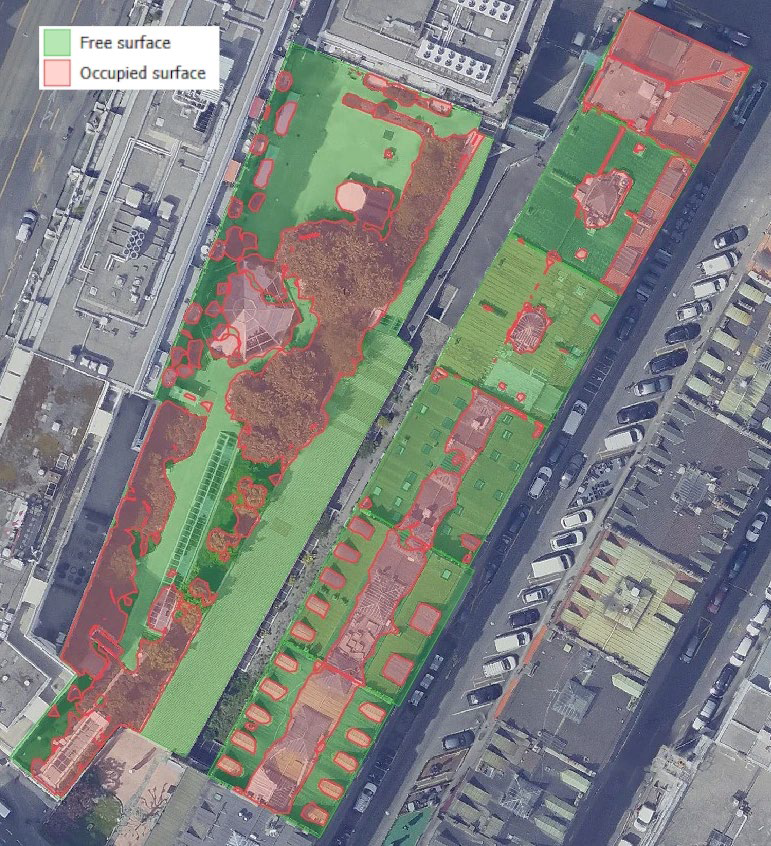
\includegraphics[width=1\linewidth]{02-main//figures/ch2/stdl_05_exemple_segmentation_lidar.png}
    \caption{Image d’exemple de la segmentation \gls{lidar} \cite{herny_detection_2024}}
    \label{fig:stdl_05_exemple_segmentation_lidar}
\end{figure}
\newpage
\par{L'algorithme obtient un F1-score de 0.77 et un mIoU (mean Intersection over Union) de 0.38 sur l'ensemble des données de test. Le Tableau \ref{tab:stdl_02_resultats_segmentation_lidar} ci-dessous résume les principales métriques obtenues.}
\begin{table}[H]
    \centering
    \begin{tabular}{|l|c|c|c|c|c|}
    \hline
    Ground truth & Precision & Recall & f1 score & mIoU & Relative error (\%) \\
    \hline
    adapted GT, training set & 0.77 & 0.77 & 0.77 & 0.42 & 11 \\
    whole GT, training set & 0.78 & 0.77 & 0.78 & 0.35 & 38 \\
    whole GT, test set & 0.75 & 0.80 & 0.77 & 0.38 & 26 \\
    \hline
    \end{tabular}
    \caption{Métriques obtenus par la segmentation \gls{lidar}}
    \label{tab:stdl_02_resultats_segmentation_lidar}
\end{table}

\par{Les objets de plus de 1 m² (Figure \ref{fig:stdl_06_segmentation_lidar_surfaces}) et situés à plus de 1 m (Figure \ref{fig:stdl_07_segmentation_lidar_distances}) du bord du toit sont bien détectés, avec des F1-score entre 0.82 et 0.92.}
\begin{figure}[H]
    \centering
    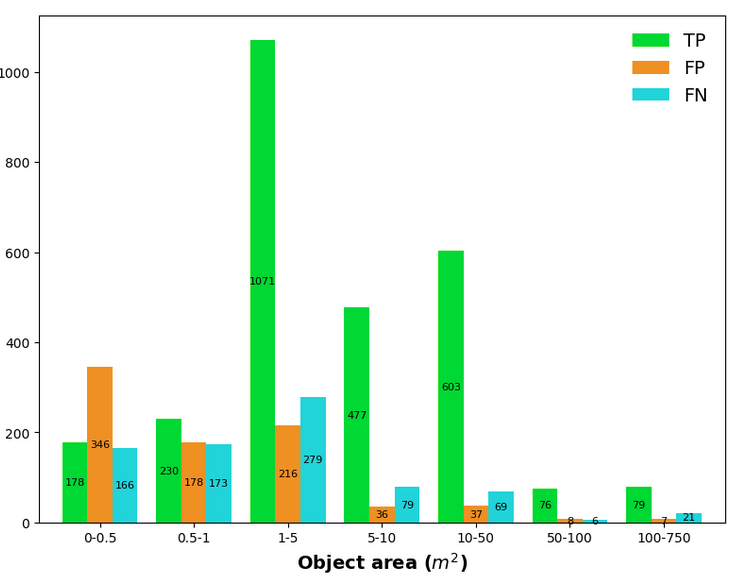
\includegraphics[width=1\linewidth]{02-main//figures/ch2/stdl_06_segmentation_lidar_surfaces.png}
    \caption{Influence de la distance des objets au bord du toit selon la surface de l’objet dans la segmentation \gls{lidar} \cite{herny_detection_2024}}
    \label{fig:stdl_06_segmentation_lidar_surfaces}
\end{figure}
\newpage
\par{Les objets (Figure \ref{fig:stdl_07_segmentation_lidar_distances}) qui ont leur centroïde a plus d'un mètre du bord du toit sont bien labellisés. Le F1-score est entre 0.80 et 0.85 pour ces objets. Cependant, les objets qui ont leur centroïde proche du bord (moins d'un mètre) ne sont pas bien détectés et ont 65\% de faux positif (FP), ce qui indique que la segmentation n'est pas fiable à cette distance.}

\begin{figure}[H]
    \centering
    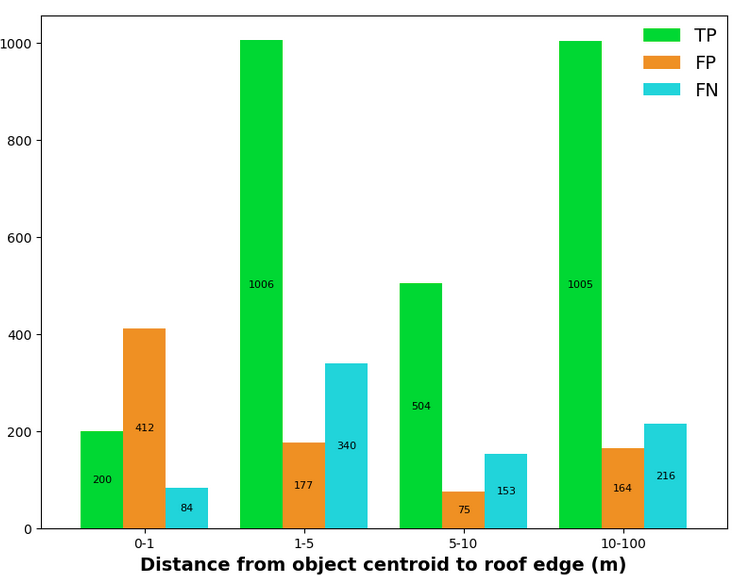
\includegraphics[width=1\linewidth]{02-main//figures/ch2/stdl_07_segmentation_lidar_distances.png}
    \caption{Influence de la distance du centre des objets au bord du toit dans la segmentation \gls{lidar} \cite{herny_detection_2024}}
    \label{fig:stdl_07_segmentation_lidar_distances}
\end{figure}
\newpage
\par{La plupart (Tableau \ref{tab:stdl_03_resultats_segmentation_lidar_classes}) des classes d'objets (bouches d'aération, balcons, végétation intensive, panneaux solaires) ont des recalls supérieurs à 0.80. Cependant, les antennes et les objets bas (fenêtres, végétation extensive, pelouses) sont plus difficiles à détecter.}

\begin{table}[H]
    \centering
    \begin{tabular}{|l|c|}
    \hline
    Object class & Recall \\
    \hline
    Antenna & 0.24 \\
    Pipe & 0.59 \\
    Lawn & 0.70 \\
    Other obstacle & 0.70 \\
    Extensive vegetation & 0.72 \\
    Window & 0.76 \\
    Chimney & 0.79 \\
    Aero & 0.83 \\
    Solar thermal & 0.83 \\
    Intensive vegetation & 0.88 \\
    Solar unknown & 0.89 \\
    Balcony / terrace & 0.90 \\
    Solar photovoltaic & 0.92 \\
    \hline
    \end{tabular}
    \caption{Recall par classe pour la segmentation LiDAR (STDL, 2024)}
    \label{tab:stdl_03_resultats_segmentation_lidar_classes}
\end{table}

\par{La surface occupée (Tableau \ref{tab:stdl_04_resultats_segmentation_lidar_affectation}) totale est sous-estimée de 38\% par rapport à la vérité terrain.}

\begin{table}[H]
    \centering
    \begin{tabular}{|p{2.7cm}|c|c|c|c|c|c|}
    \hline
    & Administrative & Industrial & Residential & Flat & Mixed & Pitched \\
    \hline
    Area labeled as occupied & 4,986 & 32,720 & 19,399 & 54,875 & 1,386 & 844 \\
    Area detected as occupied & 1,195 & 20,953 & 12,986 & 30,980 & 3,052 & 1,102 \\
    Detection rate (\%) & 24\% & 64\% & 67\% & 56\% & 220\% & 131\% \\
    Total area & 6,692 & 78,011 & 33,278 & 108,415 & 5,018 & 4,584 \\
    \hline
    \end{tabular}
    \caption{Récapitulatif des surfaces détectées et vérité terrain pour la segmentation \gls{lidar}}
    \label{tab:stdl_04_resultats_segmentation_lidar_affectation}
\end{table}


\newpage
\par{Les experts (Tableau \ref{tab:stdl_05_resultats_segmentation_lidar_experts}) sont au moins partiellement satisfaits par plus de 69\% des toits segmentés.}

\begin{table}[H]
    \centering
    \begin{tabular}{|l|c|c|}
    \hline
    Evaluation & OCAN & OCEN \\
    \hline
    Not satisfied & 22\% & 31\% \\
    Partially satisfied & 54\% & 33\% \\
    Satisfied & 24\% & 36\% \\
    \hline
    \end{tabular}
    \caption{Evaluation des experts pour la segmentation \gls{lidar}}
    \label{tab:stdl_05_resultats_segmentation_lidar_experts}
\end{table}

\paragraph{Discussion des résultats (\acrshort{stdl})}
\par{La méthode prouve sa capacité à détecter les objets sur les toits, en particulier ceux de grande taille et éloignés des bords. Cependant, la délimitation précise des formes reste perfectible, comme en témoigne le faible mIoU. L'estimation de la surface occupée est moyenne, avec une erreur importante liée à la sous-détection des objets bas. Les faux positifs sont souvent de petite taille et situés près des bords, parfois à cause de l'absence de barrières dans la vérité terrain.}
\par{Les bâtiments administratifs et les toits en pente posent des difficultés spécifiques, nécessitant des hyperparamètres adaptés.}
\par{Malgré des résultats honorables, l'aspect visuel des détections reste à améliorer pour une utilisation opérationnelle par les experts. Des développements futurs pourraient inclure l'automatisation de la production de la couche vectorielle des toits et l'ajustement de formes géométriques simples sur les clusters de points pour obtenir des détections plus précises et esthétiques.}

\newpage
\subsubsection{Segmentation d'image}

\paragraph{Données}

\par{Les données utilisées sont :}
\begin{itemize}
    \item True orthophotos \cite{sitg_orthophotos_nodate}
    \item Couche vectorielle des toitures modifiée comme pour la segmentation \gls{lidar}
\end{itemize}

\paragraph{Méthodologie}
La Figure \ref{fig:stdl_08_methodo_segmentation_images} ci-dessous représente les principales étapes utilisées pour réaliser la segmentation d'image.
\begin{figure}[H]
    \centering
    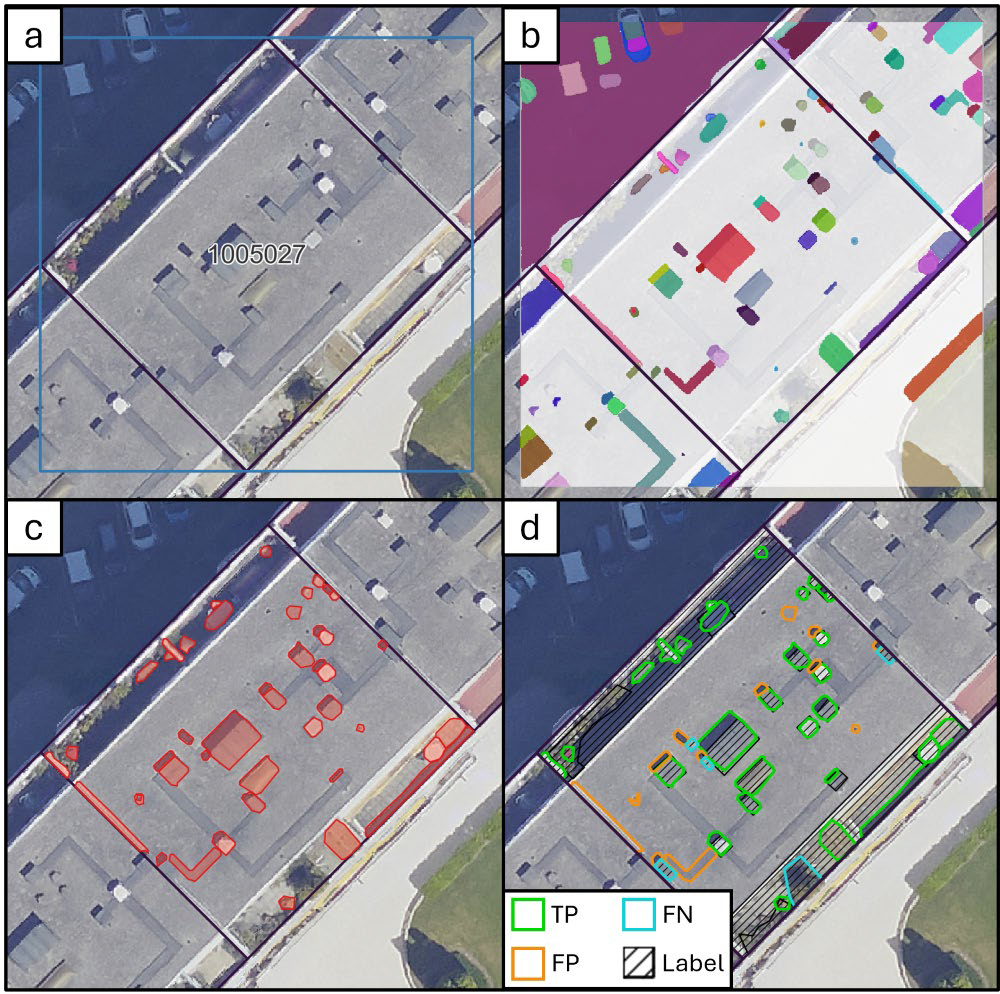
\includegraphics[width=1\linewidth]{02-main//figures/ch2/stdl_08_methodo_segmentation_images.png}
    \caption{Méthodologie pour la segmentation d’images \cite{herny_detection_2024}}
    \label{fig:stdl_08_methodo_segmentation_images}
\end{figure}

\par{La première étape est la préparation des orthophotos (Figure \ref{fig:stdl_08_methodo_segmentation_images} ``a''). Celle-ci commence par le découpage des orthophotos avec les données vectorielles des toitures (délimitation des toitures) pour ne conserver que la toiture à segmenter. La ligne bleue représente la marge de 1 mètre (zone tampon) pour faciliter la tâche de l'algorithme. Ensuite chaque toiture fera l'objet d'une tuile (une toiture par image).}

\par{La deuxième étape est la segmentation de l'image (Figure \ref{fig:stdl_08_methodo_segmentation_images} ``b''). Le modèle segment anything model (SAM) est utilisé via la librairie Python ``segment-geospatial'' \cite{wu_samgeo_2023} car cette libraire permet d'utiliser SAM sur des orthophotos tout en conservant les données géospatiales. SAM va segmenter les objets sur la toiture dans chaque tuile, ce qui va produire un masque par objet segmenté.}

\par{La troisième étape est la vectorisation des objets (Figure \ref{fig:stdl_08_methodo_segmentation_images} ``c''). Dans cette étape, les masques segmentés sont convertis en données vectorielles. Certains de ces polygones sont supprimés basé sur des critères géométriques :}
\begin{itemize}
    \item Polygone de moins de 0.2 m²
    \item Polygones qui occupent plus de 90\% de la surface de la toiture
    \item Polygones qui ont une surface de plus de 50\% de la toiture et qui n'ont pas d'intersection avec la toiture
\end{itemize}

\par{La quatrième étape est l'optimisation des hyperparamètres (Figure \ref{fig:stdl_08_methodo_segmentation_images} ``d'') de SAM et l'évaluation de ses résultats avec la vérité terrain.}

\par{La logique est que tout ce qui n'est pas segmenté à l'intérieur du périmètre de la toiture est une surface libre.}

\newpage
\paragraph{Résultats}

\par{La Figure \ref{fig:stdl_09_segmentation_image_resultats} représente un exemple de résultat de la segmentation de plusieurs toitures. On peut observer que la segmentation rencontre des difficultés avec certains éléments de toiture tel que les puits de lumière.}
\begin{figure}[H]
    \centering
    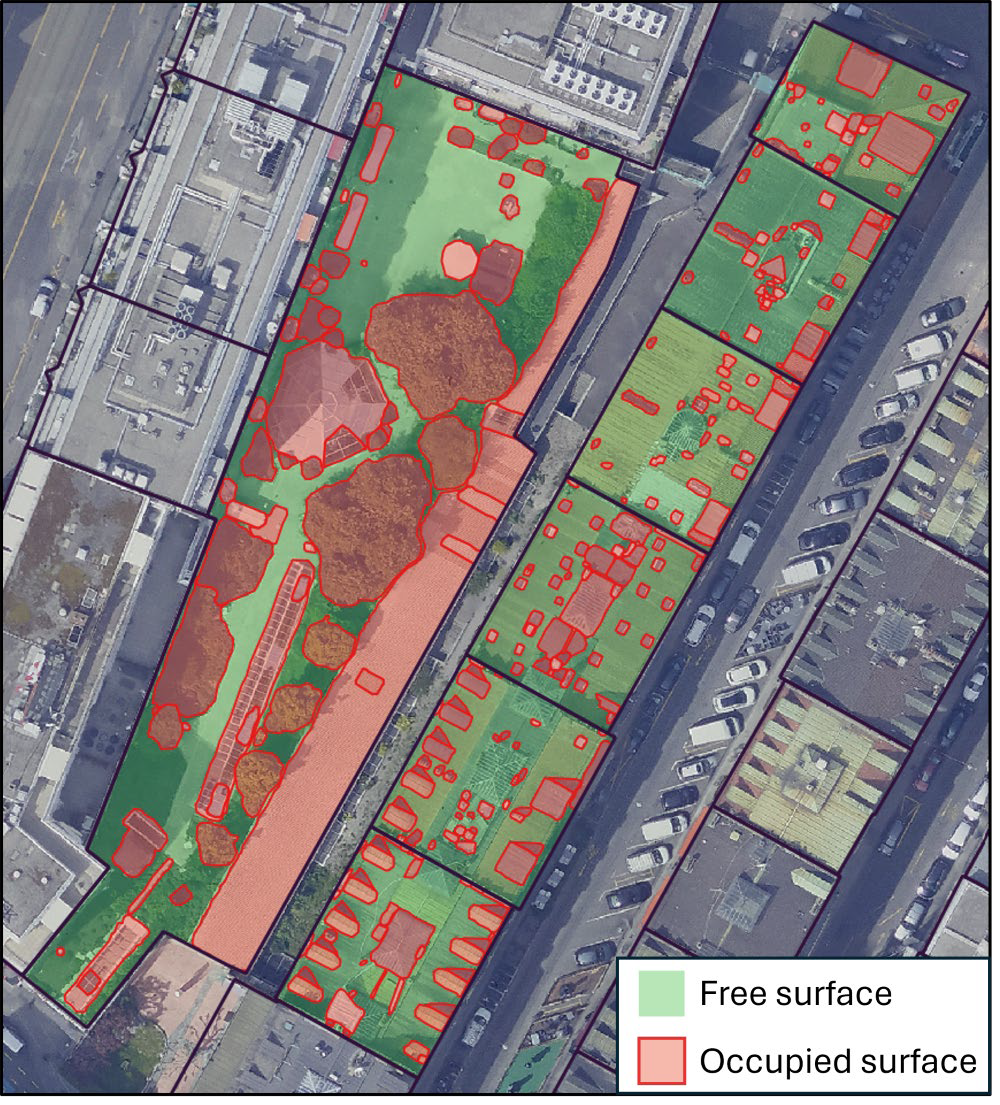
\includegraphics[width=1\linewidth]{02-main//figures/ch2/stdl_09_segmentation_image_resultats.png}
    \caption{Exemple d’image résultat de la segmentation d’images \cite{herny_detection_2024}}
    \label{fig:stdl_09_segmentation_image_resultats}
\end{figure}
\newpage
\par{Les métriques obtenues (Tableau \ref{tab:stdl_06_segmentation_image_resultats}) sur le dataset de test sont un F1-score de 0.73 et mIoU de 0.37.}
\begin{table}[H]
    \centering
    \begin{tabular}{|l|c|c|c|c|c|}
    \hline
    Dataset & Precision & Recall & f1 score & mIoU & Relative error (\%) \\
    \hline
    Training subset & 0.73 & 0.78 & 0.75 & 0.41 & 7 \\
    Training & 0.75 & 0.82 & 0.78 & 0.37 & 42 \\
    Test & 0.75 & 0.71 & 0.73 & 0.37 & 23 \\
    \hline
    \end{tabular}
    \caption{Métriques obtenues par la segmentation d'images}
    \label{tab:stdl_06_segmentation_image_resultats}
\end{table}
\par{Les petits objets (Figure \ref{fig:stdl_10_segmentation_image_taille}) avec une surface de moins d'un mètre carré sont moins bien détectés (AP d'environ 0.60). Les objets de plus d'un mètre carré sont mieux détectés (AP d'environ 0.83).}
\begin{figure}[H]
    \centering
    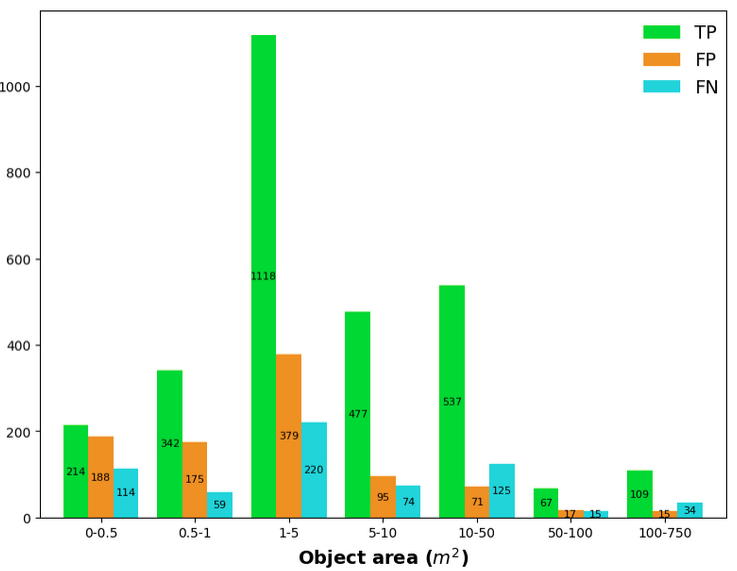
\includegraphics[width=1\linewidth]{02-main//figures/ch2/stdl_10_segmentation_image_taille.png}
    \caption{Objets segmentés selon taille en m² pour la segmentation d’images \cite{herny_detection_2024}}
    \label{fig:stdl_10_segmentation_image_taille}
\end{figure}
\newpage
\par{Comme pour la segmentation \gls{lidar}, la segmentation d'image fonctionne moins bien au bord de la toiture (Figure \ref{fig:stdl_11_segmentation_image_distance}). La precision est de 0.77 pour les centroïde d'objets a plus d'un mètre du bord de la toiture contre seulement 0.51 pour ceux a moins d'un mètre.}

\begin{figure}[H]
    \centering
    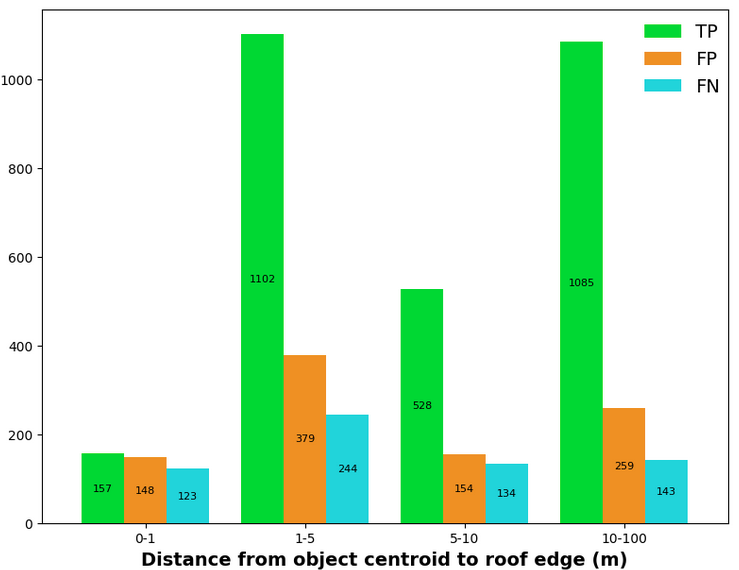
\includegraphics[width=1\linewidth]{02-main//figures/ch2/stdl_11_segmentation_image_distance.png}
    \caption{Centroïde des objets segmentés selon la distance au borde de la toiture pour la segmentation d’images  \cite{herny_detection_2024}}
    \label{fig:stdl_11_segmentation_image_distance}
\end{figure}

\par{Les experts sont au minimum partiellement satisfait de 86\% des résultats (Tableau .}
\begin{table}[h]
    \centering
    \begin{tabular}{|l|c|c|}
    \hline
    Evaluation & OCAN & OCEN \\
    \hline
    Not satisfied & 6\% & 14\% \\
    Partially satisfied & 40\% & 49\% \\
    Satisfied & 54\% & 37\% \\
    \hline
    \end{tabular}
    \caption{Evaluation des experts pour la segmentation d'images (STDL, 2024)}
    \label{tab:stdl_07_segmentation_image_resultats_experts}
\end{table}
\newpage
\paragraph{Discussion résultats (\acrshort{stdl})}

\par{Points forts de cette approche :}
\begin{itemize}
\item Bonne capacité générale à détecter et segmenter correctement les objets
\item Métriques cohérentes
\item Forme des objets détectés généralement bien reproduite
\end{itemize}

\par{Limites constatées de la méthodologie utilisée :}
\begin{itemize}
\item Difficulté à détecter les objets tel que les gaines ou d'autres petits objets
\item Sensibilité aux changements de couleurs (saleté, ombres, pans de toit) pouvant être interprétés comme des objets
\item Temps de calcul important (12 minutes pour 25 bâtiments), mise à l'échelle du canton (plus de 80'000 bâtiments) compliquée
\item Nécessité des true orthophotos, plus rares et coûteuses que les orthophotos standards
\end{itemize}

\par{Potentielles améliorations :}
\begin{itemize}
\item Fine-tuning du modèle SAM
\item Méthodes pour atténuer la présence d'ombres dans les images
\item Adaptation de la méthodologie pour utiliser des orthophotos standard
\end{itemize}

\subsubsection{Combinaison}

\par{Ce chapitre va traiter la combinaison des résultats de 2 méthodologies différentes pour améliorer les résultats finaux.}

\paragraph{Données}

\par{Les données utilisées sont le résultat des méthodologies de segmentation \gls{lidar} et celui de la segmentation d'images. Ce sont des données vectorielles.}

\paragraph{Méthodologie}

\par{Deux méthodes de combinaison des résultats ont été testées.}

\par{La première est la concaténation des objets détectés à partir des couches vectorielles produites par les segmentations \gls{lidar} et d'images.}

\par{La deuxième est la jointure spatiale des résultats de la segmentation \gls{lidar} et d'images. Dans ce cas, il faut :}
\begin{itemize}
    \item Sélectionner les polygones qui se chevauchent entre les couches vectorielles des segmentations \gls{lidar} et d'images.
    \item Conserver les polygones issus de la segmentation d'images car ils fournissent une meilleure délimitation
\end{itemize}
\newpage
\paragraph{Résultats}

\par{Les couches vectorielles obtenues n'ont pas été évaluées par les experts. Le Tableau \ref{tab:stdl_08_ensemble_resultats} ci-dessous résume les principales métriques obtenues.}

\begin{table}[H]
    \centering
    \begin{tabular}{|l|c|c|c|c|c|}
    \hline
    Combination method & Precision & Recall & f1 score & mIoU & Relative error (\%) \\
    \hline
    Concatenation & 0.68 & 0.94 & 0.79 & 0.45 & 8 \\
    Spatial join & 0.81 & 0.69 & 0.75 & 0.33 & 48 \\
    \hline
    \end{tabular}
    \caption{Métriques obtenues par les méthodes de combinaison}
    \label{tab:stdl_08_ensemble_resultats}
\end{table}

\par{En complément du Tableau \ref{tab:stdl_08_ensemble_resultats}, le Tableau \ref{tab:stdl_09_resultats_methodos} récapitule l'ensemble des métriques des méthodologies. La méthodologie de classification des pans de toit n'a pas de métrique, elle n'est donc pas incluse dans le tableau.}

\begin{table}[H]
    \centering
    \begin{tabular}{|l|c|c|c|c|c|}
    \hline
    Méthodologie & Precision & Recall & F1-score & mIoU & Relative error [\%] \\
    \hline
    Segmentation \gls{lidar} & 0.75 & 0.80 & 0.77 & 0.38 & 26 \\
    Segmentation d'image & 0.75 & 0.71 & 0.73 & 0.37 & 23 \\
    Concaténation & 0.68 & 0.94 & 0.79 & 0.45 & 8 \\
    Jointure spatiale & 0.81 & 0.69 & 0.75 & 0.33 & 48 \\
    \hline
    \end{tabular}
    \caption{Comparatif des résultats des différentes méthodologies}
    \label{tab:stdl_09_resultats_methodos}
\end{table}

\par{Les F1-scores des deux méthodes de combinaison sont proches, autour de 0.77, ce qui suggère des performances globales similaires.}

\par{La concaténation obtient un recall exceptionnel de 0.94, détectant presque toutes les surfaces occupées. En contrepartie, la précision diminue d'environ 8 points, indiquant plus de faux positifs dans les résultats.}

\par{La jointure spatiale fait le choix inverse : elle améliore la précision de 6 points en réduisant les détections erronées, mais perd 8 points de recall, manquant davantage de surfaces réellement occupées.}

\par{Le mIoU favorise nettement la concaténation avec un gain de plus de 10 points, reflétant une segmentation de meilleure qualité. Cette tendance se confirme pour l'estimation des surfaces : la concaténation maintient l'erreur relative sous 10\% tandis que la jointure spatiale atteint environ 50\%.}

\paragraph{Discussion des résultats (\acrshort{stdl})}

Les points positifs de cette approche sont :
\begin{itemize}
    \item La combinaison des résultats permet de moduler les résultats en favorisant soit la précision soit le recall selon les besoins
    \item La valeur élevée du recall obtenue par concaténation prouve la complémentarité des deux méthodes pour détecter différents objets
\end{itemize}

\par{La valeur de recall élevée obtenue avec la concaténation prouve la complémentarité des deux méthodes pour la détection d'objets différents. Une valeur de recall plus élevée tend à favoriser le mIoU, puisque plus d'objets sont détectés (TP), malgré l'ajout de faux positifs (FP). La surface de l'objet détecté est donc améliorée, mais l'ajout de FP contribue également à la réduction de l'erreur relative sur la surface occupée, ce qui doit être analysé avec soin.}

\par{L'utilisation des couches vectorielles des toits et superstructures produites par l'État de Genève, bien qu'incomplètes, pourrait améliorer les résultats.}

\subsubsection{Conclusion}

\par{\acrshort{stdl} a exploré trois méthodes pour détecter les objets sur les toits à partir de données \gls{lidar}, d'orthophotos et vectorielles. Toutes les méthodes ont fourni des résultats satisfaisants, avec une précision de 85\% pour la classification d'occupation et un F1-score d'environ 0,77 pour les méthodes de segmentation. Les bénéficiaires ont été satisfaits des résultats dans au moins 70\% des cas.}

\par{La méthode de classification a été sélectionnée en raison de ses bonnes performances et résultats obtenus.}

\par{La combinaison des résultats de segmentation permet d'améliorer soit la précision, soit le recall, et le croisement des sources d'information peut améliorer la précision des résultats.}

\par{Il est important de noter que ces résultats sont des indications qui doivent être vérifiées par un expert métier. Des paramètres supplémentaires, tels que le matériau du toit et le potentiel solaire, ne sont pas pris en compte.}

\subsubsection{Analyse critique}

\paragraph{Général}

\par{Le projet étant encore dans sa phase initiale explorative, il ne tient pas compte de l'orientation des toitures pour évaluer le potentiel solaire de chacune d'entre elle. L'exposition au soleil est en effet un facteur essentiel pour la pose de panneaux solaire. L'exclusion de toitures sur la base des données du cadastre solaire pourrait éventuellement éviter de traiter les toitures à l'ombre.}

\par{La végétalisation de toitures impose des défis considérables d'un point de vue génie civil, en effet les toitures ne sont souvent pas prévues pour porter des charges tel que de la terre végétale. Même dans le cas des panneaux solaires, pas toutes les toitures peuvent supporter la charge. Par exemple une toiture en fibrociment (toiture typique des hangars) n'aura probablement pas la capacité pour accueillir des panneaux solaires, cela pourrait être un critère d'exclusion.}

\par{L'échantillon de bâtiments du dataset ne semble pas très équilibré entre les différentes classes \gls{sia} de bâtiments \cite{sia_sia-shop_nodate}. En effet, les piscines couvertes, écoles, dépôts, hôpitaux ont pas mal en commun en ce qui concerne les toitures, elles seront probablement plates avec des éléments de ventilation ou froid. Les logements collectifs sont probablement plus complexes à segmenter car en général les toitures sont déjà assez occupées.}

\paragraph{Classification des pans de toiture}

\par{Les données de la couche vectorielle d'emprise au sol des bâtiments ne donnent pas un aperçu complet de la toiture, en effet les superstructures se trouvent dans une autre couche vectorielle. Même si ce n'est pas mentionné, les deux couches ont probablement été fusionnées.}

\par{Dans le rapport de \acrshort{stdl}, il manque une matrice de confusion. Cela aurait permis d'avoir une meilleure appréciation des performances obtenues par les différentes variantes utilisées.}

\paragraph{Segmentation \gls{lidar}}

\par{Le choix d'utiliser les données \gls{lidar} de 2019 avec les orthophotos de 2019 est tout à fait logique. Des données \gls{lidar} plus récentes et avec plus de densité existent mais il n'y a pas de true orthophoto après 2019 qui servirait de vérité terrain. Cela enlèverait aussi la possibilité de comparer les différents modèles de segmentation sur des données similaires.}

\paragraph{Segmentation d'images}

\par{La stratégie utilisée pour la segmentation d'images est très futée. La stratégie est principalement :}
\begin{itemize}
    \item Segmentation avec SAM
    \item Enlever certains masques trop petits ou qui sont en dehors de la toiture
    \item Tout ce qui n'a pas de masque devient donc une surface disponible
\end{itemize}

\par{\acrshort{stdl} l'a déjà indiqué dans son rapport, après avoir expérimenté avec SAM, il est tout de même très sensible aux ombrages. L'approche fonctionne moyennement bien avec un mIoU de 0.37.}

\par{En revanche, la stratégie de faire une tuile par toiture semble compliquée et le temps nécessaire est relativement long (12 minutes pour 25 bâtiments).}

\par{La segmentation à l'aide d'un algorithme de machine learning supervisé semble plus pertinente, l'inférence d'une image prend moins d'une minute pour un modèle de type YOLO et celle-ci peut contenir plusieurs bâtiments.}

\paragraph{Combinaison des résultats}

\par{\acrshort{stdl} n'a pas inclus dans leur rapport un tableau qui récapitule les résultats des différentes méthodologies utilisées. C'est donc difficile d'avoir une idée des résultats globaux.}

\paragraph{Résultats}

\par{Le Tableau \ref{tab:stdl_09_resultats_methodos} permet d'avoir une vue d'ensemble des résultats et la concaténation est fort intéressante.}

\par{La concaténation des résultats des deux méthodes de segmentation (\gls{lidar} et image) permet d'obtenir un recall élevé, ce qui signifie que la grande majorité des objets présents dans la vérité terrain (GT) sont détectés. Ce recall élevé s'explique par le fait que les deux méthodes ont des forces complémentaires : chacune est capable de détecter des types d'objets différents que l'autre méthode peut manquer.}

\par{Par exemple, la segmentation d'image peut mieux détecter les objets fins et bas, tandis que la segmentation \gls{lidar} peut mieux gérer les changements de couleur et détecter les gaines.}

\par{Un recall plus élevé a tendance à améliorer la métrique mIoU (mean Intersection over Union), car davantage d'objets GT sont correctement détectés (vrais positifs, TP), même si cela s'accompagne également de l'ajout de faux positifs (FP). Le mIoU mesure la qualité de la segmentation en calculant le chevauchement moyen entre les objets détectés et les objets GT. Avec plus de TP, le numérateur du mIoU augmente, ce qui améliore le score global.}

\par{De plus, un recall élevé permet une meilleure estimation de la surface occupée par les objets détectés. Cependant, l'ajout de FP lors de la concaténation peut également contribuer à cette surface occupée, ce qui peut réduire artificiellement l'erreur relative par rapport à la surface occupée réelle (calculée à partir de la GT). Il est donc important d'interpréter ce résultat avec prudence, car une faible erreur relative sur la surface occupée ne signifie pas nécessairement que la segmentation est parfaite, mais peut être influencée par la présence de FP.}

% -----------------------------------------------------------------------------
\subsection{SolarNet plus}
\label{subsec:solar_net_plus}

\subsubsection{Contexte et objectifs}
\par{\citeauthor{li_deep_2024} présentent SolarNet+ \cite{li_deep_2024}, un framework basé sur l'apprentissage profond qui vise à estimer avec précision le potentiel solaire des toitures urbaines. Cet article est la suite de l'article \cite{li_solarnet_2023} SolarNet par les mêmes auteurs principaux}
\par{Contrairement aux méthodes existantes, SolarNet+ prend en compte simultanément l'orientation des toits et les superstructures présentes (cheminées, fenêtres, etc.) qui réduisent la surface disponible pour l'installation de panneaux solaires. Cette approche permet d'éviter une surestimation du potentiel solaire et offre une évaluation plus précise pour soutenir la planification énergétique durable et les objectifs de neutralité carbone.}

\subsubsection{Données}
\par{L'étude utilise principalement le jeu de données RID (Roof Information Dataset). Le dataset est décrit en détail dans la sous-section \ref{subsec:rid_roof_information_dataset}.}
\par{Le dataset consiste en 1880 images satellite en provenance de google. Les images disposent des annotations suivantes:
\begin{itemize}
    \item Les segments de toiture et leur orientation (plat, N, E, S, W)
    \item Éléments de toiture
    \begin{itemize}
        \item Panneau PV
        \item Lucarne
        \item Fenêtre
        \item Échelle
        \item Cheminée
        \item Ombrage
        \item Arbre/végétation
        \item Fond d'image (background)
        \item Inconnu
    \end{itemize}
\end{itemize}}
\par{La Figure \ref{fig:rid_dataset_sample} représente une image d'exemple ainsi que ses annotations. Le jeu de données est divisé en dataset d'entraînement (70\%), de validation (10\%) et de test (20\%).}
\begin{figure}[H]
    \centering
        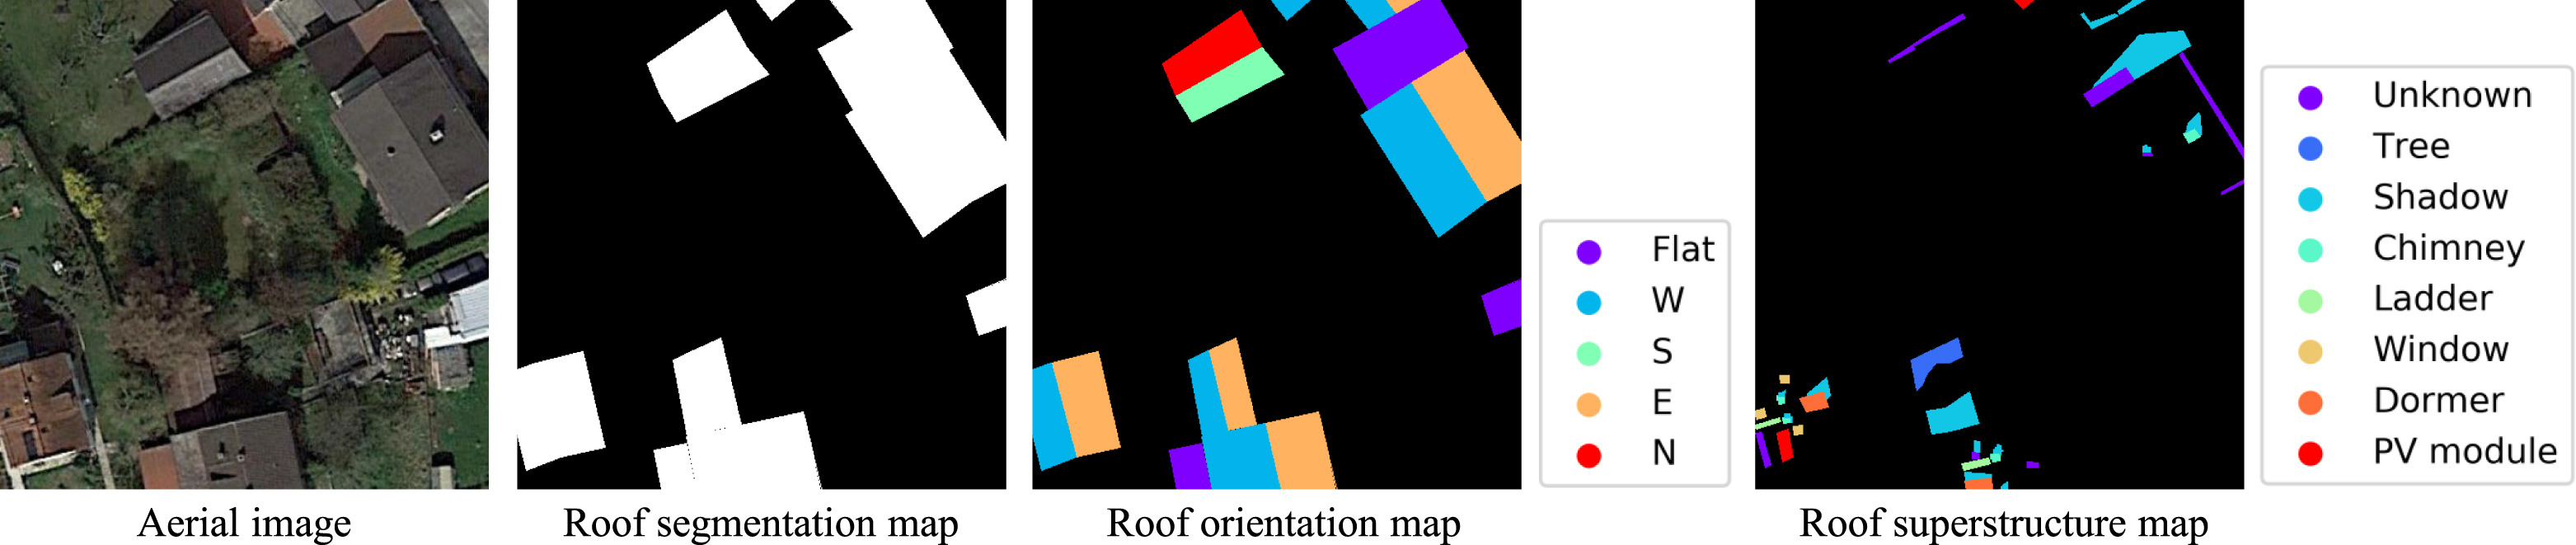
\includegraphics[width=1\linewidth]{02-main//figures/ch2/rid_dataset_sample.png}
    \caption{Exemple d'image du dataset RID \cite{li_deep_2024}}
    \label{fig:rid_dataset_sample}
\end{figure}

\subsubsection{Méthodologie}
\par{SolarNet+ utilise une approche en deux étapes :}
\begin{enumerate}
    \item Un réseau de neurones multi fonctions (partie 1 de la Figure \ref{fig:solar_net_plus_methodo}) va réaliser les opérations suivantes sur chaque image:
    \begin{itemize}
        \item Segmenter l'image pour avoir le masque de la toiture ainsi que son orientation géographique ("Roof orientation map" de la Figure \ref{fig:solar_net_plus_methodo}).
        \item Segmenter les éléments de toiture pour identifier tous les obstacles qui s'y trouvent ("Roof superstructure map" de la Figure \ref{fig:solar_net_plus_methodo}).
        \item Extraire les surfaces exploitables de toiture par superposition des masques. Cette étape consiste à soustraire les zones occupées par les obstacles ("Roof superstructure map") des segments de toiture identifiés ("Roof orientation map"), permettant ainsi d'isoler les surfaces disponibles.
    \end{itemize}
    \item Estimer le potentiel solaire pour chaque surface identifiée (partie 2 de la Figure \ref{fig:solar_net_plus_methodo}) qui comprend :
    \begin{itemize}
        \item Hypothèses de base pour le calcul :
        \begin{itemize}
            \item Panneau PV 1.7 \si{\unit{\square\meter}} avec 400 Wc
            \item Pente toiture 30° pour toutes les orientations sauf toiture plate 0°
            \item Pans de toiture de moins de 5 \si{\unit{\square\meter}} ne sont pas considérés comme surface disponible
        \end{itemize}
        \item Calcul du nombre maximum de panneaux installables sur chaque segment de toiture disponible, en tenant compte des contraintes géométriques. La Figure \ref{fig:solar_net_plus_placement_pv}) présente deux exemples, avec et sans obstacles sur la toiture. Le placement des panneaux commence du côté gauche en bas et va éviter les obstacles présents.
        \item Acquisition des données d'irradiation solaire spécifiques à chaque orientation via l'API PVGIS
        \item Estimation de l'énergie annuelle générée pour chaque pans de toiture en multipliant le nombre de panneaux installables par la production unitaire correspondant à l'orientation
        \item Additionner les potentiels de tous les pans de toiture pour obtenir le potentiel solaire total du bâtiment
    \end{itemize}
\end{enumerate}

\begin{figure}[H]
    \makebox[\textwidth][c]{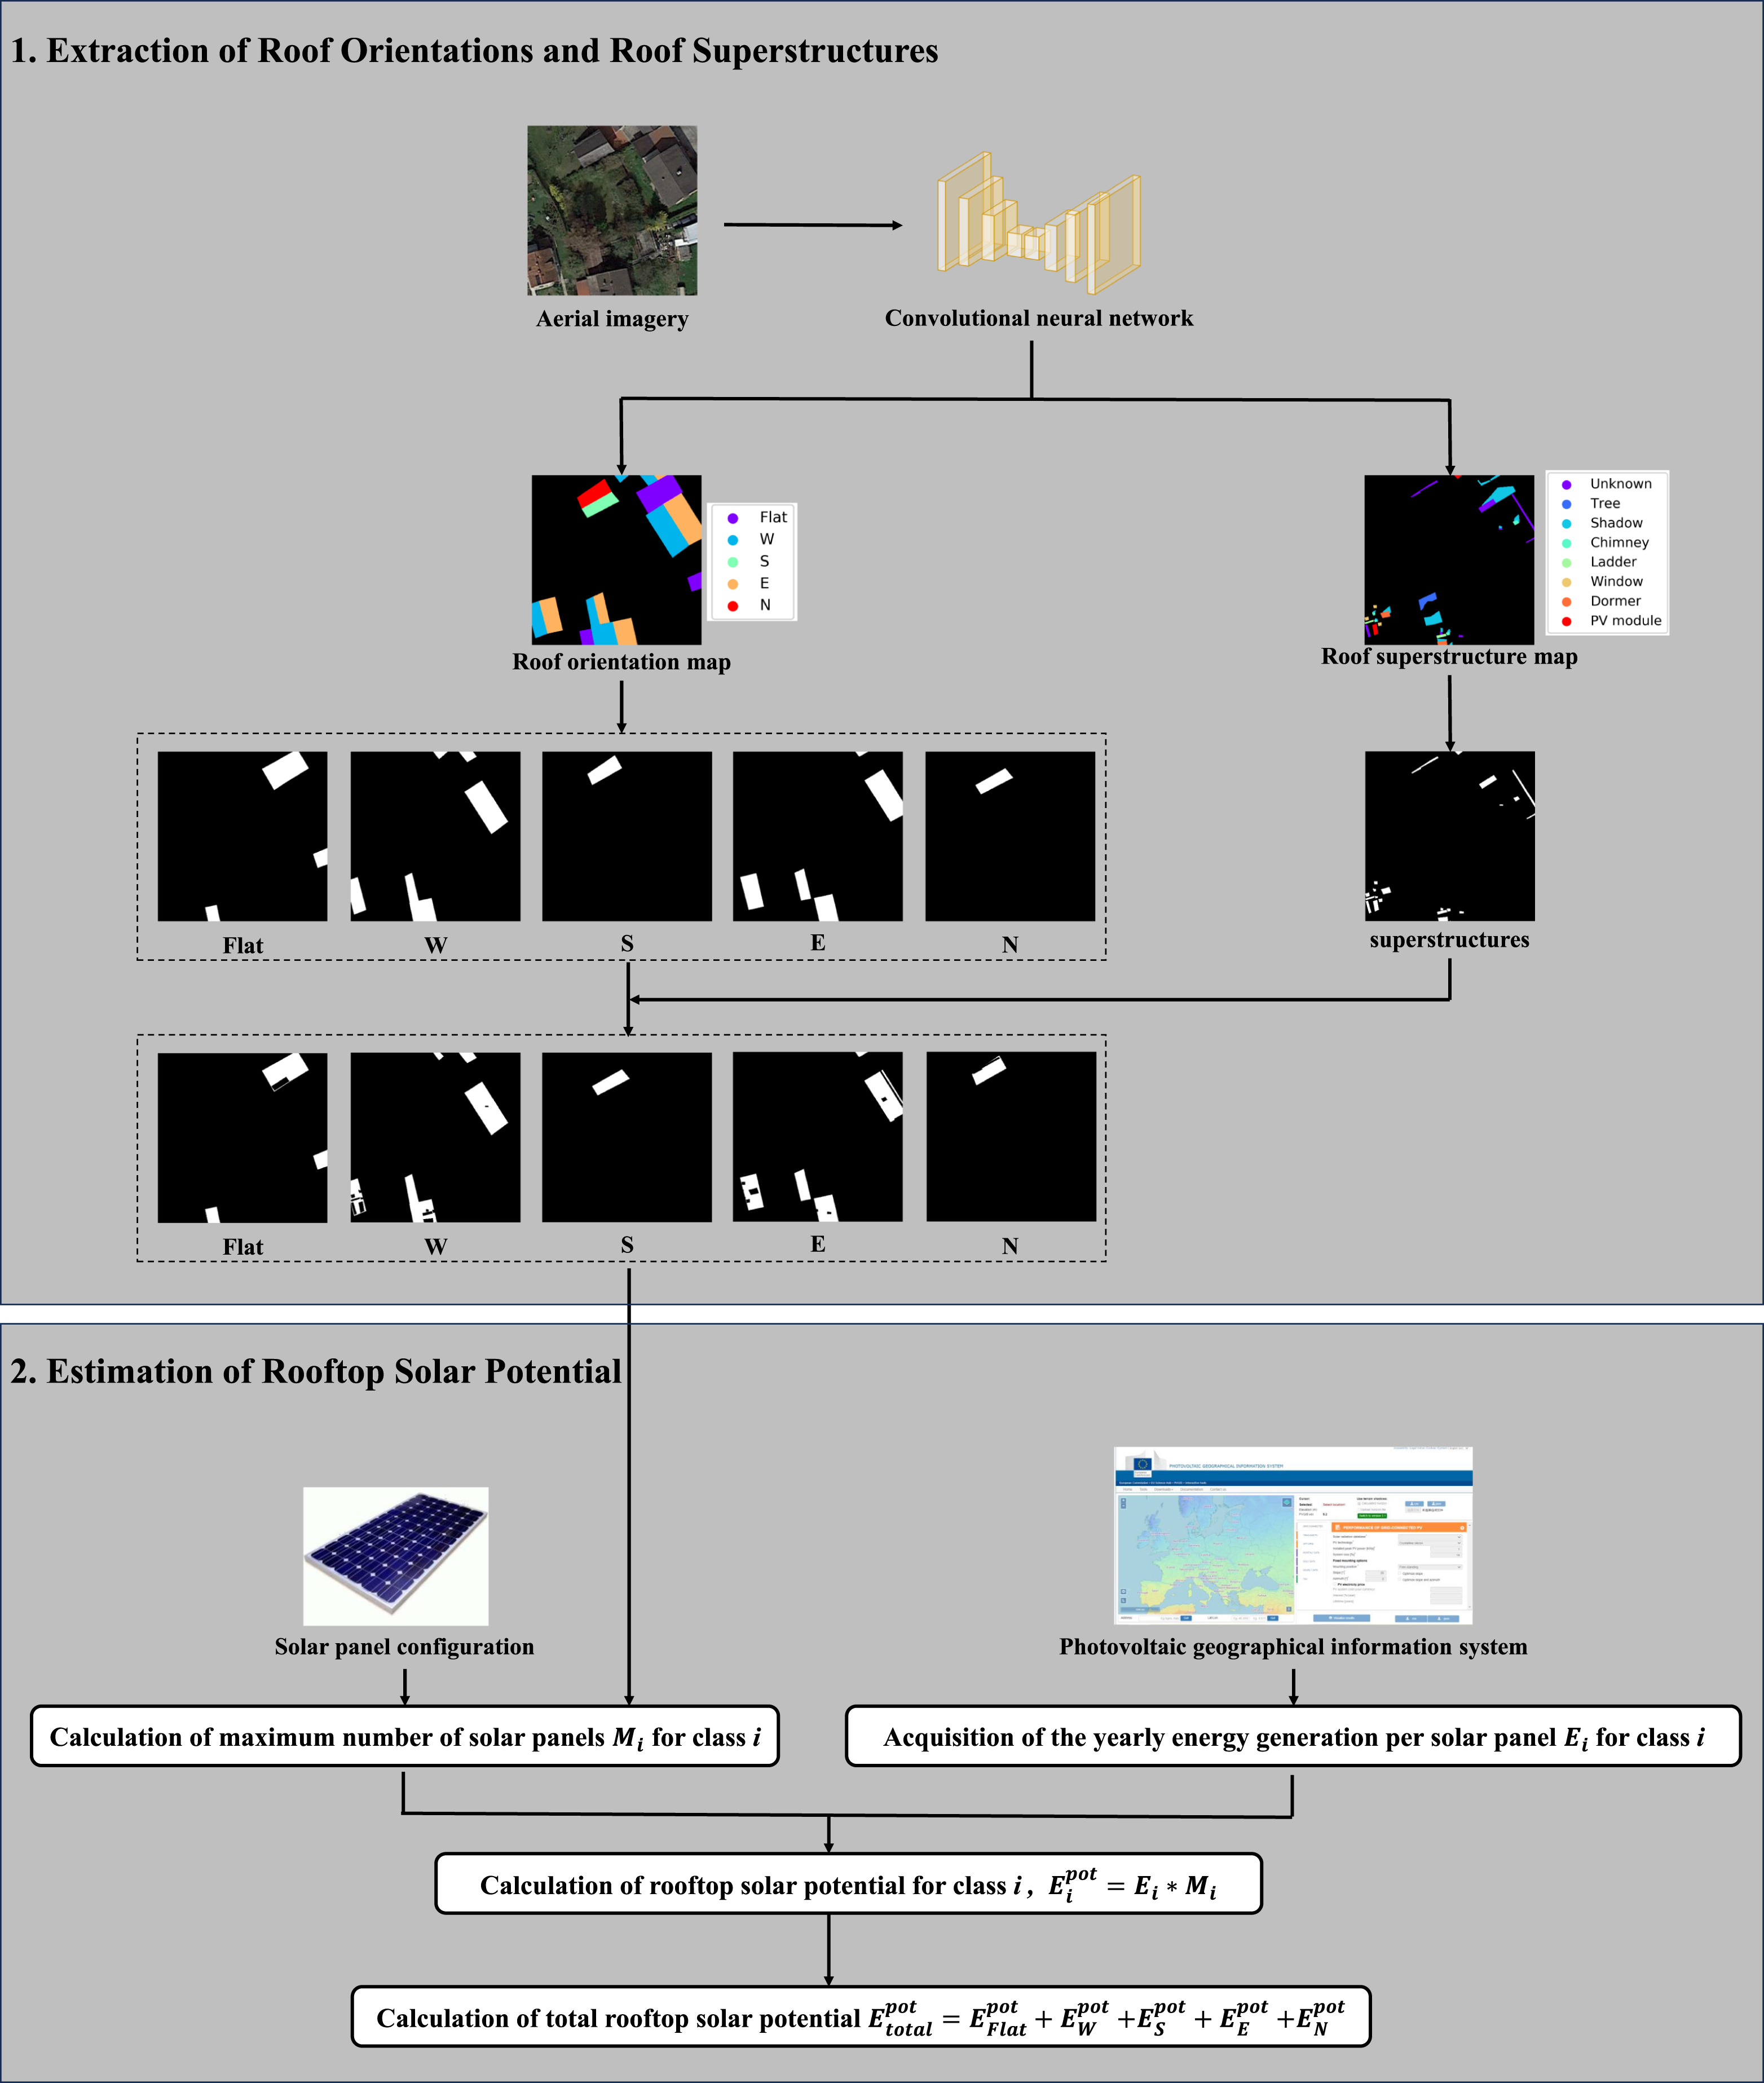
\includegraphics[width=1.1\textwidth]{02-main//figures/ch2/solar_net_plus_methodo.png}}
    \caption{Méthodologie SolarNet+ \cite{li_deep_2024}}
    \label{fig:solar_net_plus_methodo}
\end{figure}

\begin{figure}[H]
    \centering
    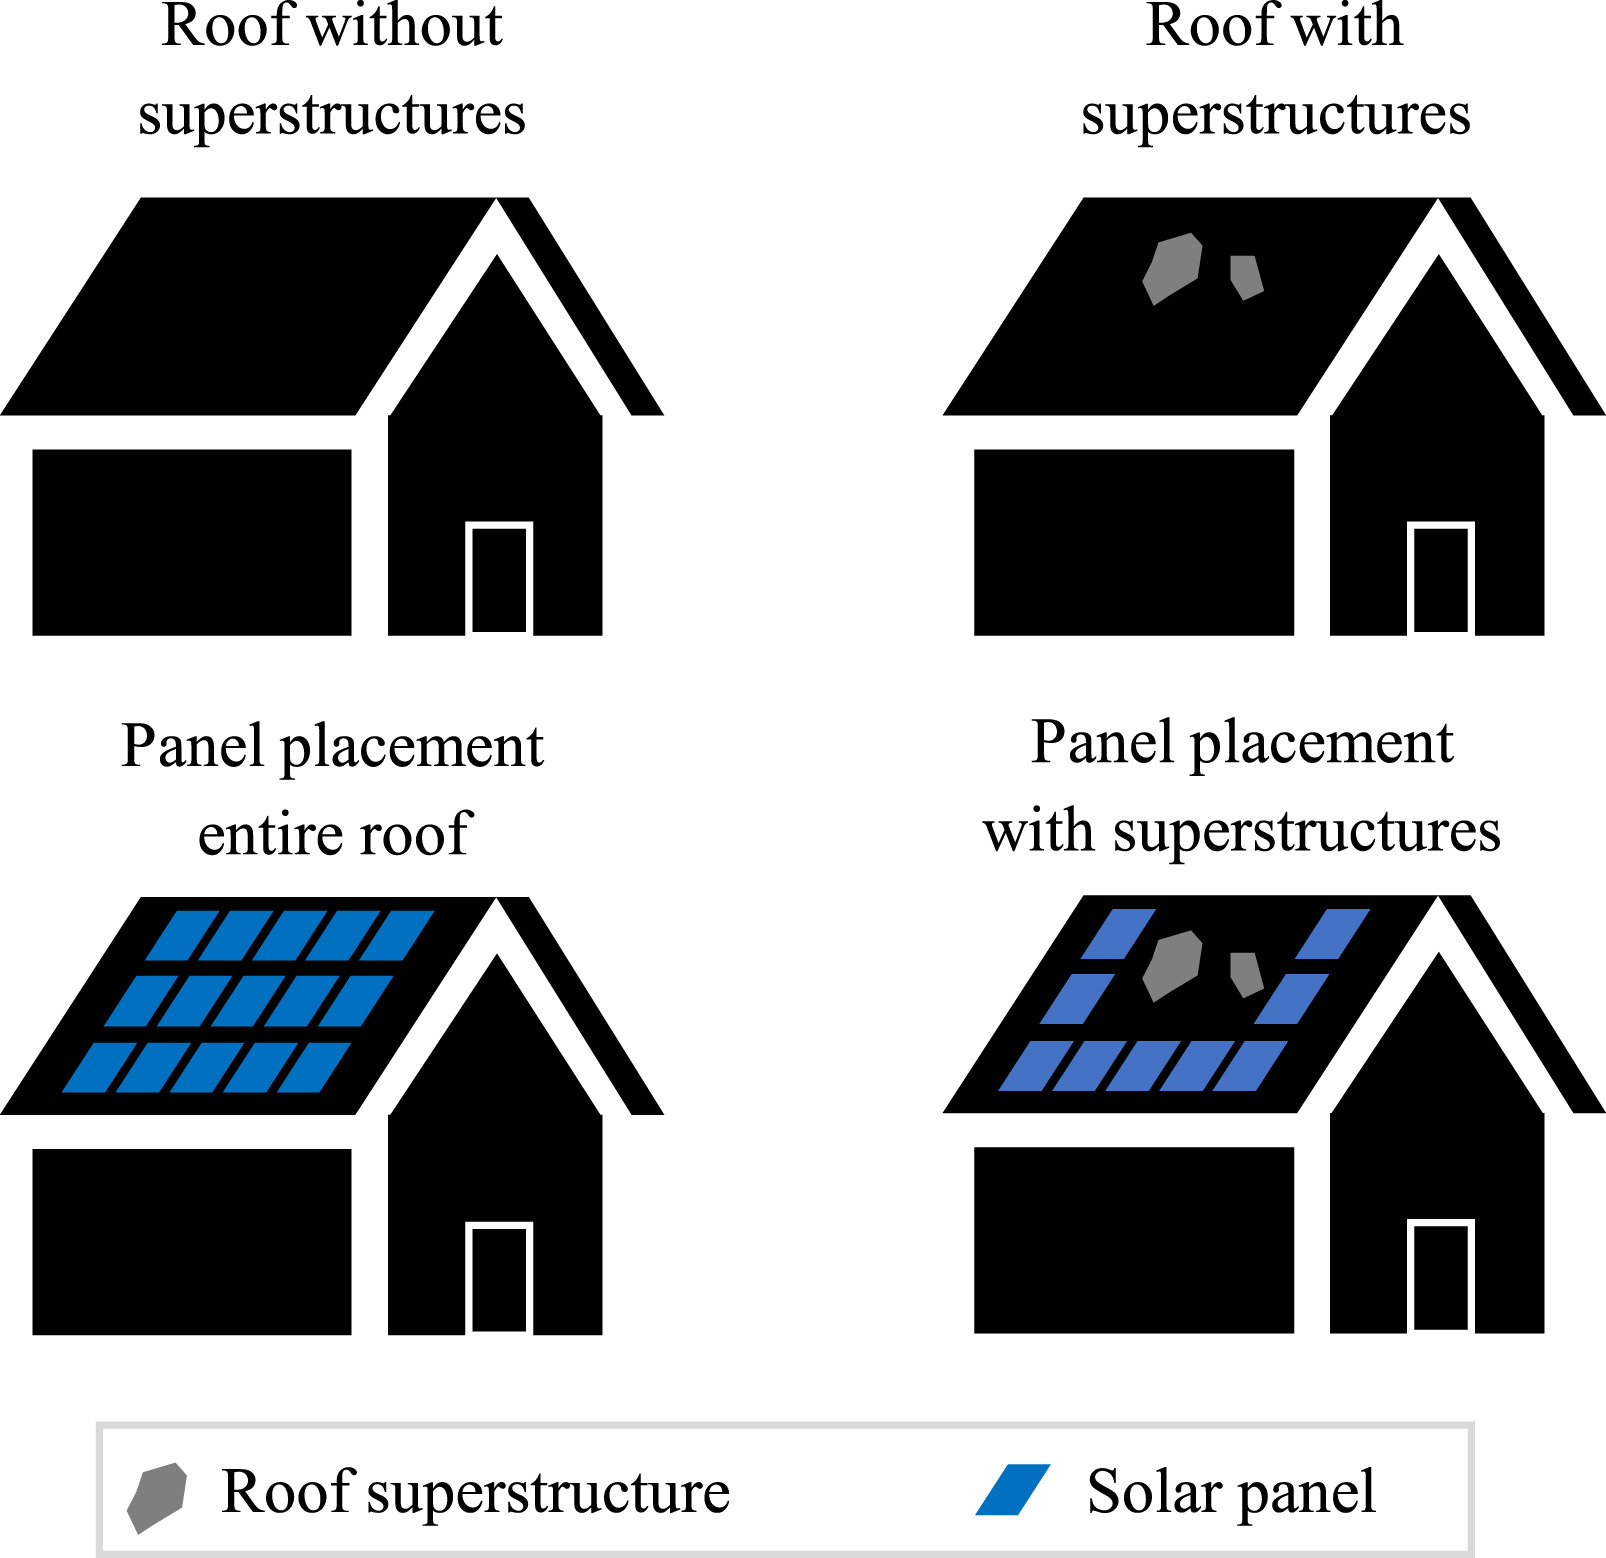
\includegraphics[width=0.5\linewidth]{02-main//figures/ch2/solar_net_plus_placement_pv.png}
    \caption{Placement des panneaux solaire \cite{li_deep_2024}}
    \label{fig:solar_net_plus_placement_pv}
\end{figure}

\par{La Figure \ref{fig:solar_net_plus_exemple_methodo} permet d'avoir un aperçu des différentes phases du calcul de potentiel solaire. En allant de gauche à droite dans la lecture de la Figure \ref{fig:solar_net_plus_exemple_methodo}, les deux premières images indiquent l'irradiation solaire avec et sans les obstacles. En bas à gauche de ces deux images, on peut observer une toiture avec plusieurs obstacles détectés (trous), sans les obstacles son irradiation solaire est bonne, mais avec les obstacles son irradiation solaire totale est réduite. La troisième image représente le placement des panneaux solaires. Finalement la quatrième image, représente le potentiel solaire total par pan de toiture selon le nombre de panneaux solaire placés dans la troisième image et l'irradiation solaire de la deuxième image.}

\begin{figure}[H]
    \makebox[\textwidth][c]{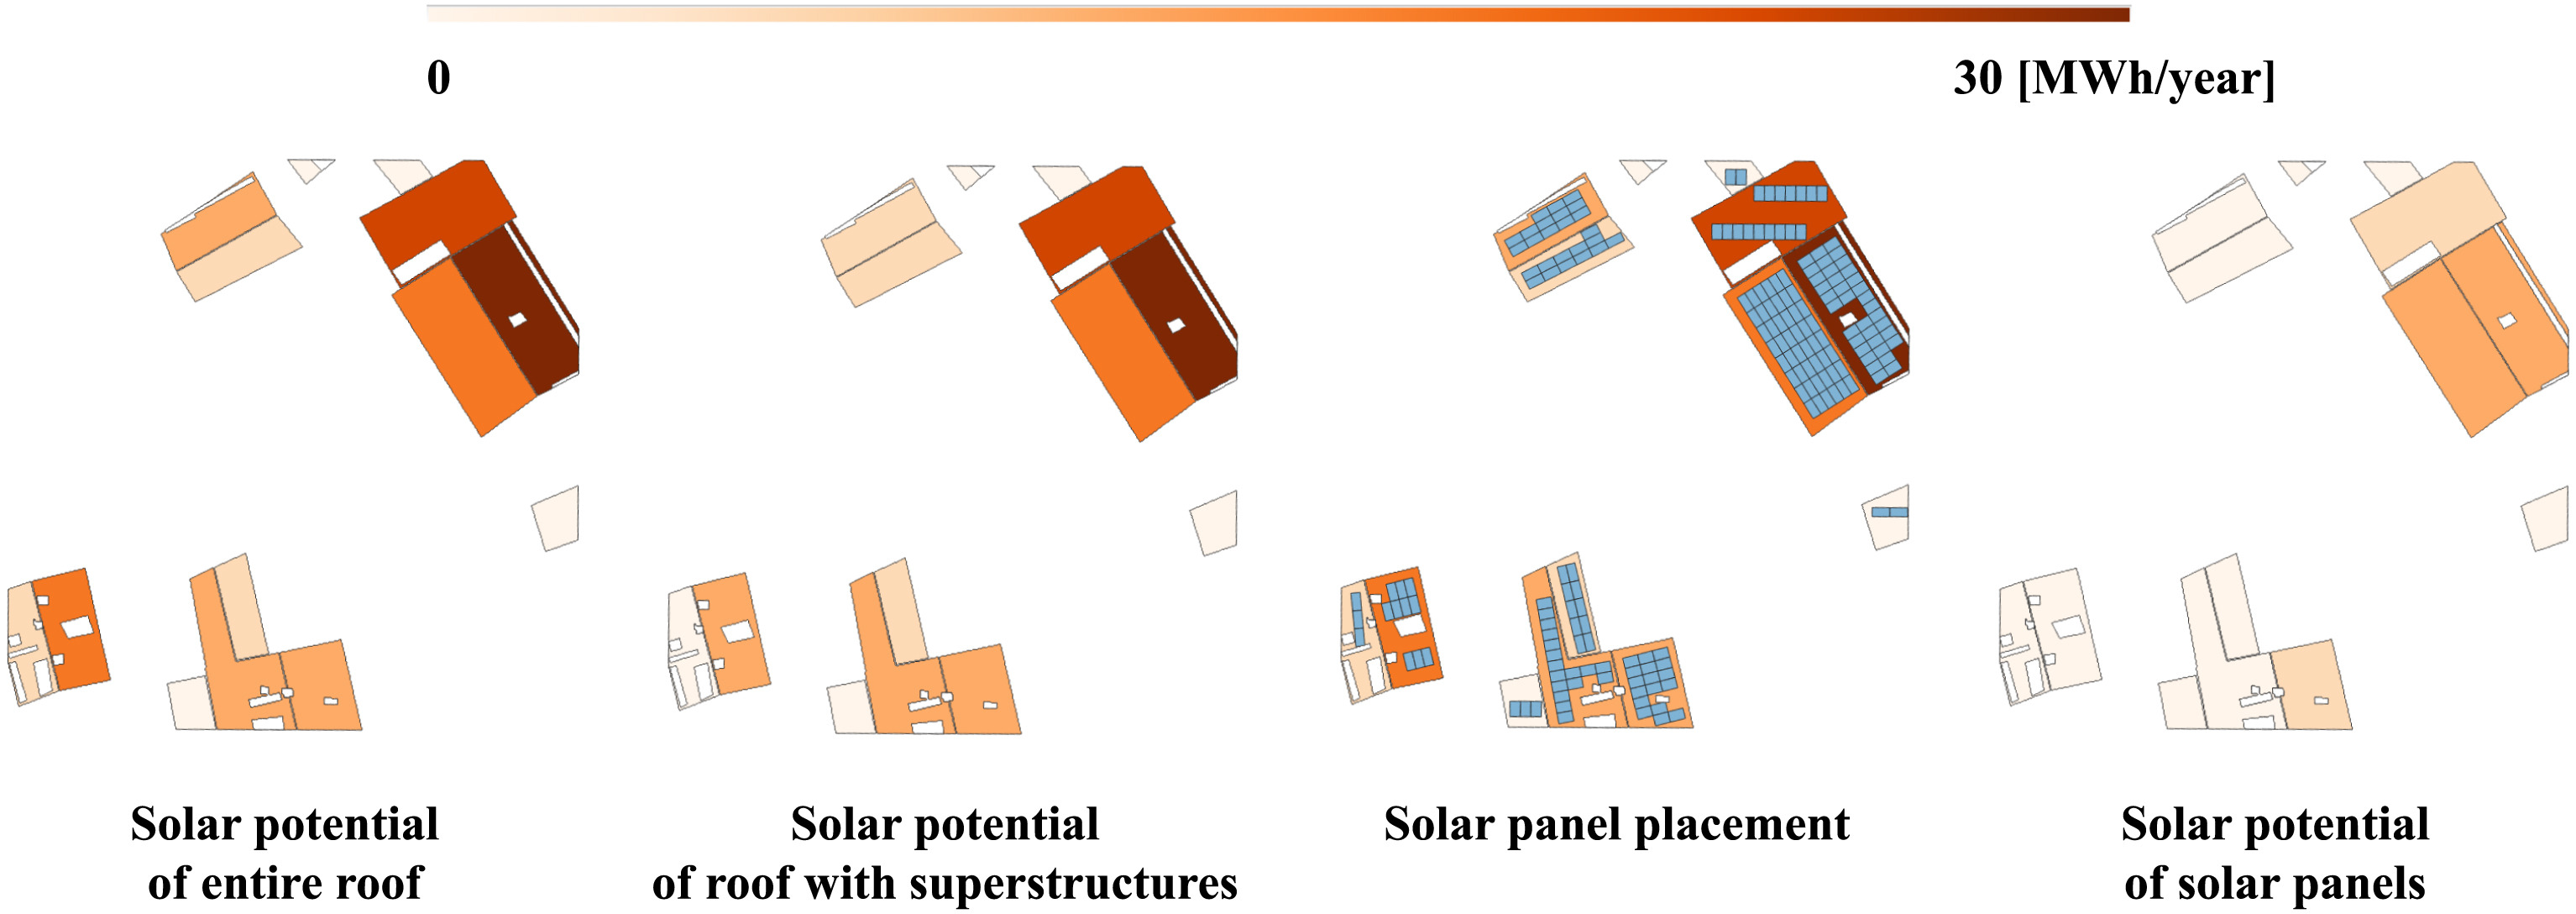
\includegraphics[width=1.15\textwidth]{02-main//figures/ch2/solar_net_plus_exemple_methodo.png}}
    \caption{Exemple d'application de la méthodologie \cite{li_deep_2024}}
    \label{fig:solar_net_plus_exemple_methodo}
\end{figure}

\subsubsection{Résultats principaux}
\begin{itemize}
    \item SolarNet+ surpasse les réseaux concurrents en termes de précision pour la prédiction de l'orientation des toits et des superstructures avec les meilleures performances en mIoU et OA.
    \item L'étude montre que négliger les superstructures conduit à une surestimation de 42\% du nombre de panneaux solaires installables.
    \item La précision d'estimation du potentiel solaire atteint un \%RMSE de 19,92\% par rapport la vérité terrain (détail des résultats dans la Table \ref{tab:solar_net_plus_comparaison_quant}).
\end{itemize}

\begin{table}[H]
    \centering
    \small
    \begin{tabular}{lrrrr}
        \toprule
        \textbf{Méthode} & \textbf{Nombre de panneaux} & \textbf{Potentiel solaire} & \textbf{RMSE} & \textbf{\%RMSE} \\
        & \textbf{installables} & \textbf{(MWh/an)} & \textbf{(MWh/an)} & \\
        \midrule
        U-Net & 25 855 & 8484,28 & 12,77 & 21,49 \\
        FC-DenseNet & 29 316 & 9544,90 & 20,85 & 35,10 \\
        Efficient-UNet & 23 842 & 7754,68 & 16,85 & 28,37 \\
        DeepLab V3+  & 28 152 & 9153,37 & 25,14 & 42,32 \\
        Srivastava et al. & 24 987 & 8125,64 & 12,63 & 21,27 \\
        Bischke et al. & 25 749 & 8446,82 & 14,34 & 24,13 \\
        Mou \& Zhu & 24 945 & 8075,86 & 14,22 & 23,93 \\
        \textbf{SolarNet+} & \textbf{24 541} & \textbf{7967,34} & \textbf{11,83} & \textbf{19,92} \\
        \midrule
        Ground truth & 24 279 & 7959,76 & - & - \\
        \bottomrule
    \end{tabular}
    \caption{Résultats quantitatifs du potentiel solaire sur le dataset RID \cite{li_deep_2024}}
    \label{tab:solar_net_plus_comparaison_quant}
\end{table}


\subsubsection{Discussion et limites}
\begin{itemize}
    \item La démarche utilisée par cet article est assez unique, c'est le seul article qui va aussi loin dans la segmentation des toitures et l'identification des obstacles. Le dataset RID est disponible librement et il a été réalisé par les auteurs de cet article.
    \item Les auteurs ont testé le modèle avec des images satellite de Bruxelles (le dataset RID inclus seulement Wartenberg à Munich), mais les performances diminuent en raison des différences architecturales et des superstructures non rencontrées dans les données d'entraînement (balcons, éléments technique de ventilation/climatisation, etc.).
    \item Le modèle ne prend pas en compte les ombrages, ce qui peut réduire significativement l'irradiation solaire reçue par un pan de toiture.
    \item Les auteurs suggèrent d'intégrer des données 3D et cela semble une bonne initiative pour des futures évolutions du framework. Avec des données \gls{lidar}, ils pourraient nettement améliorer la phase de post-processing des pans de toiture en intégrant les ombrages et une meilleure estimation des pentes des toitures.
\end{itemize}

% -----------------------------------------------------------------------------
\subsection{Quantification of the suitable rooftop area for solar panel installation from overhead imagery using Convolutional Neural Networks}
\label{subsec:castello_quantification_2021}

\subsubsection{Contexte et objectifs}
\par{Cet article \cite{castello_quantification_2021} présente une approche innovante pour quantifier les surfaces disponibles sur les toitures pour l'installation de panneaux solaires photovoltaïques. Face au défi de l'évaluation précise du potentiel solaire à grande échelle, \citeauthor{castello_quantification_2021} proposent une méthode combinant le deep learning, la vision par ordinateur et des données de bâtiments 3D.}

\subsubsection{Méthodologie}
\par{L'approche utilise un réseau de neurones convolutif (CNN) basé sur l'architecture U-Net, adapté pour la segmentation sémantique d'images aériennes à haute résolution. Le modèle a été entraîné sur 524 images (orthophotos de swisstopo 2015) de taille 250x250 pixels de Genève, avec une résolution spatiale de 0,25 m/pixel. Les données d'entraînement ont été annotées manuellement (classe unique "libre") pour identifier les zones disponibles sur les toits. Ces données ne sont pas disponibles.}

\par{La méthodologie comporte trois étapes principales :}
\begin{enumerate}
    \item Traitement des images aériennes par le CNN pour identifier les surfaces disponibles
    \item Post-traitement géospatial combinant les résultats avec la couche \acrshort{sitg} des toitures
    \item Les toitures de moins de 10 \si{\unit{\square\meter}} ne sont pas considérées comme toiture disponible
\end{enumerate}

\par{Les auteurs ont également implémenté diverses techniques d'augmentation de données et optimisé les hyperparamètres du modèle pour améliorer ses performances.}

\subsubsection{Résultats principaux}
Le CNN développé atteint :
\begin{itemize}
    \item Une précision de 93\% dans l'identification des surfaces disponibles
    \item Un score d'Intersection over Union (IoU) de 64\%
    \item Une sous-estimation moyenne de 8\% des surfaces disponibles par rapport aux annotations manuelles
\end{itemize}
\par{Le Tableau \ref{tab:castello_quantification_resultats} ci-dessous détaille les résultats obtenus:}
\begin{table}[H]
    \centering
    \begin{tabular}{|l|c|c|c|c|c|}
    \hline
     & IoU & Accuracy & Recall & Precision & F1-score \\
    \hline
    Training & 0.8823 & 0.9794 & 0.9299 & 0.9437 & 0.9367 \\
    Validation & 0.7211 & 0.9464 & 0.8360 & 0.8508 & 0.8433 \\
    Test & 0.6420 & 0.9307 & 0.7522 & 0.7874 & 0.7693 \\
    \hline
    \end{tabular}
    \caption{Performances du modèle U-Net développé}
\label{tab:castello_quantification_resultats}
\end{table}

\par{Le modèle réussit à détecter automatiquement les obstacles présents sur les toits, y compris les panneaux solaires existants, fenêtres, cheminées, équipements techniques et zones ombragées. L'étude révèle que la fraction médiane de la surface disponible varie selon la taille des toits :}
\begin{itemize}
    \item 61\% pour les grands toits (>500 m²)
    \item 77\% pour les toits moyens (100-500 m²)
    \item 80\% pour les petits toits (10-100 m²)
\end{itemize}

\par{La Figure \ref{fig:castello_quantification_image_resultat} permet de voir deux exemples de résultat.}
\begin{figure}[H]
    \centering
    \begin{subfigure}{0.44\textwidth}
        \centering
        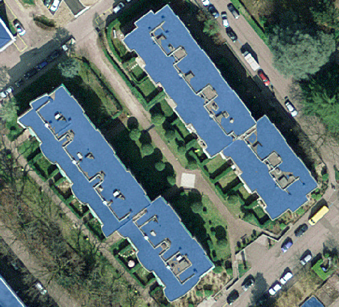
\includegraphics[width=\textwidth]{02-main//figures/ch2/castello_quantification_image_resultat1.png}
        \caption{Grandes toitures plates}
        \label{fig:castello_quantification_image_resultat1}
    \end{subfigure}
    \hfill
    \begin{subfigure}{0.43\textwidth}
        \centering
        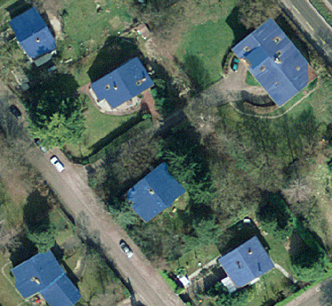
\includegraphics[width=\textwidth]{02-main//figures/ch2/castello_quantification_image_resultat2.png}
        \caption{Toitures en pente}
        \label{fig:castello_quantification_image_resultat2}
    \end{subfigure}
    \caption{Images d'exemple \cite{castello_quantification_2021} du résultat après inférence. Les zones bleus sont les espaces disponibles.}
    \label{fig:castello_quantification_image_resultat}
\end{figure}

\par{La comparaison avec d'autres méthodes d'estimation montre que les approches existantes tendent à surestimer la surface disponible sur les grands toits et à sous-estimer celle des petits toits.}

\subsubsection{Discussion et limites}
\par{L'article présente une approche prometteuse pour quantifier les surfaces de toiture disponibles pour l'installation solaire. Le modèle U-Net atteint un IoU de 64\% et une précision de 93\% sur les données de test, avec la capacité notable d'exclure automatiquement les zones ombragées des toits.}
\par{La comparaison avec les méthodes existantes révèle des différences selon la taille des bâtiments. Pour les grandes toitures, le modèle CNN estime une fraction médiane de surface disponible de 39\% contre 66\% pour l'approche de référence, suggérant une surestimation des méthodes à grande échelle. Pour les petites toitures, la tendance s'inverse avec 47\% contre 32\%.}
\par{Le modèle sous-estime en moyenne de 8\% la surface réellement disponible par rapport à la vérité terrain. Cette sous-estimation est principalement observée sur les petites toitures (< 100 m²). Les limites identifiées incluent la difficulté à détecter les lucarnes, construites dans le même matériau que le toit, et les zones de "toits verts" avec végétation.}
\par{L'étude se limite au centre de Genève avec 524 images principalement résidentielles. Les auteurs mentionnent 12 heures de labellisation manuelle sans préciser la répartition du travail. Pour une extension nationale, ils proposent l'ajout d'un canal infrarouge et l'utilisation d'images plus récentes à haute résolution.}

% -----------------------------------------------------------------------------

\subsection{YOLOv12: Attention-Centric Real-Time Object Detectors}

\subsubsection{Contexte et objectifs}
La détection d'objets en temps réel repose traditionnellement sur les réseaux de neurones convolutionnels (CNN) dans la famille YOLO. Cependant, les mécanismes d'attention, popularisés par les ``Vision Transformers'', offrent de meilleures capacités de modélisation grâce à leur capacité à capturer les dépendances globales dans l'image. Le problème fondamental est que l'attention a un coût computationnel élevé : sa complexité croît quadratiquement avec la taille de l'image ($O(n^2)$), là où les convolutions croissent linéairement ($O(n)$). 

YOLOv12 relève ce défi en proposant le premier framework YOLO centré sur l'attention qui atteint la vitesse des modèles CNN traditionnels tout en conservant les avantages de performance de l'attention. L'objectif est de démontrer qu'il est possible de casser la domination des CNN dans YOLO.

\subsubsection{Données}
L'évaluation utilise le dataset de référence MS COCO 2017 pour la détection d'objets. Cinq variantes de modèles sont développées (YOLOv12-N/S/M/L/X) correspondant à différentes tailles et complexités. L'entraînement suit le protocole standard : 600 époques avec l'optimiseur SGD, augmentations de données classiques (Mosaic, Mixup, copy-paste). Les performances sont mesurées sur GPU T4 avec TensorRT FP16 pour assurer la reproductibilité.

\subsubsection{Méthodologie}
YOLOv12 introduit trois innovations clés pour rendre l'attention efficace :
\begin{itemize}
    \item Réduction de la complexité (Area Attention)
    \item Stabilisation de l'entraînement (R-ELAN)
    \item Améliorations architecturales
\end{itemize}

\paragraph{Area Attention (A2)}
Plutôt que de calculer l'attention sur toute l'image (coûteux), la carte de caractéristiques est divisée en zones rectangulaires (par défaut 4 segments). L'attention n'est calculée qu'à l'intérieur de chaque zone, réduisant la complexité de moitié tout en préservant un champ réceptif suffisant. C'est l'équivalent de regarder plusieurs « fenêtres » de l'image simultanément plutôt que l'image entière.

Le mécanisme d'attention (Figure \ref{fig:ch2_yolo_mecanismes_attention}) local est simplifié par rapport aux autres alternatives (Figures \ref{fig:ch2_yolo_01_attention_area_criss_cross}, \ref{fig:ch2_yolo_02_attention_area_window} et \ref{fig:ch2_yolo_03_attention_area_criss_axial}). Celui-ci divise la carte de caractéristiques en $l$ segments (par défaut 4) verticalement (Figure \ref{fig:ch2_yolo_05_attention_area_yolo2}) ou horizontalement (Figure \ref{fig:ch2_yolo_04_attention_area_yolo1}), réduisant la complexité tout en maintenant un large champ réceptif.

\begin{figure}[H]
    \centering
    \begin{subfigure}[b]{0.30\textwidth}
        \centering
        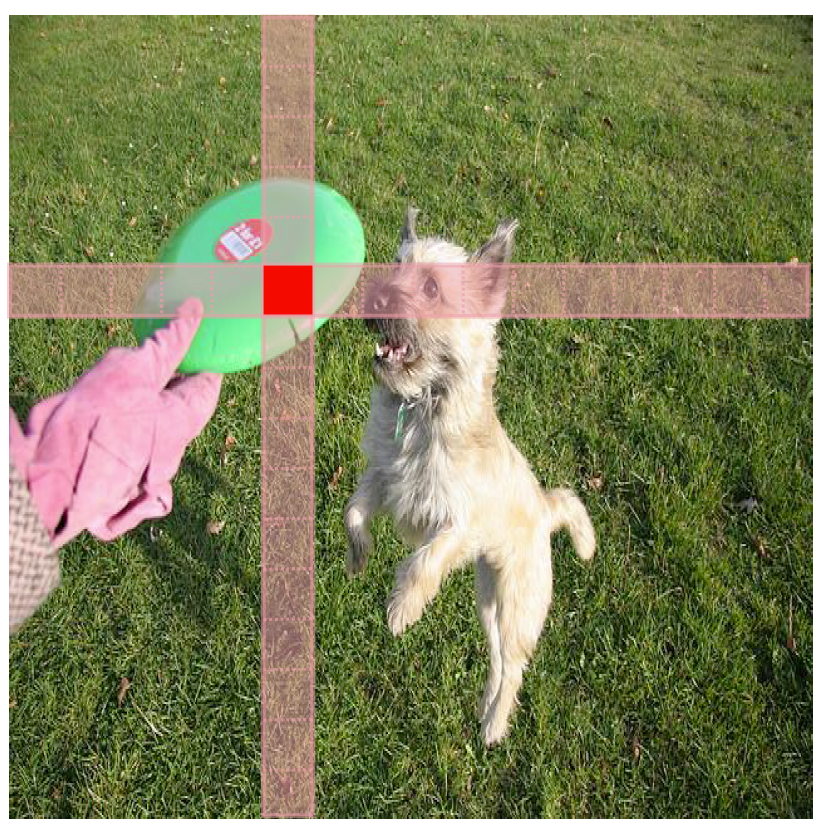
\includegraphics[width=\textwidth]{02-main/figures/ch2/ch2_yolo_01_attention_area_criss_cross.png}
        \caption{Mécanisme d'attention type ``criss cross''}
        \label{fig:ch2_yolo_01_attention_area_criss_cross}
    \end{subfigure}
    \hfill
    \begin{subfigure}[b]{0.30\textwidth}
        \centering
        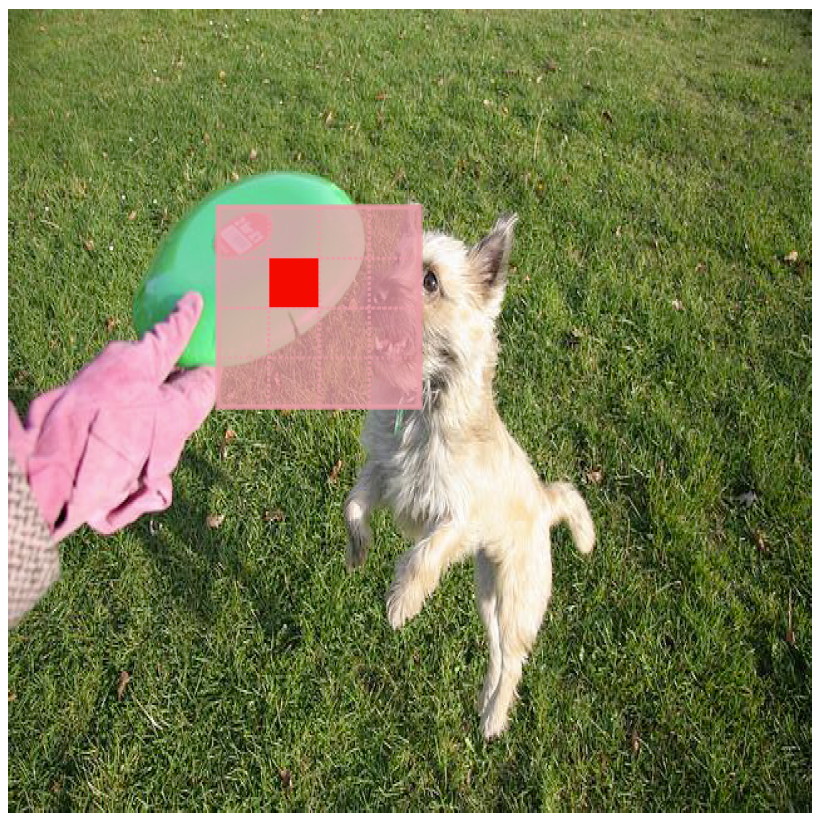
\includegraphics[width=\textwidth]{02-main/figures/ch2/ch2_yolo_02_attention_area_window.png}
        \caption{Mécanisme d'attention type ``fenêtre''}
        \label{fig:ch2_yolo_02_attention_area_window}
    \end{subfigure}
    \hfill
    \begin{subfigure}[b]{0.30\textwidth}
        \centering
        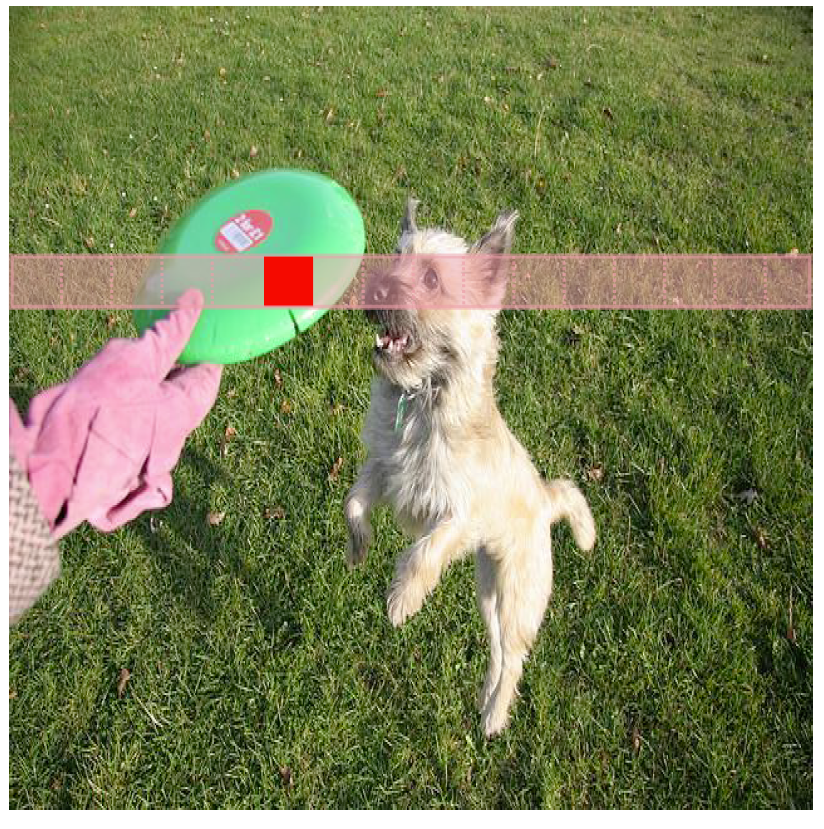
\includegraphics[width=\textwidth]{02-main/figures/ch2/ch2_yolo_03_attention_area_criss_axial.png}
        \caption{Mécanisme d'attention type ``axial''}
        \label{fig:ch2_yolo_03_attention_area_criss_axial}
    \end{subfigure}

    \vspace{0.35cm}
    \begin{subfigure}[b]{0.30\textwidth}
        \centering
        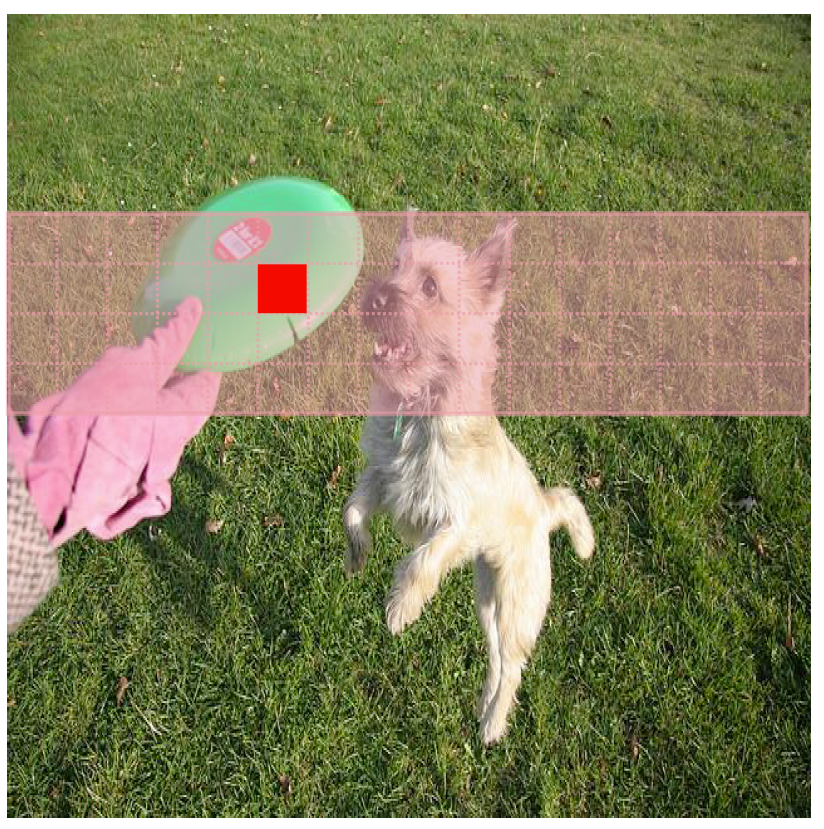
\includegraphics[width=\textwidth]{02-main/figures/ch2/ch2_yolo_04_attention_area_yolo1.png}
        \caption{Mécanisme d'attention horizontal proposé dans YOLOv12}
        \label{fig:ch2_yolo_04_attention_area_yolo1}
    \end{subfigure}
    \hspace{0.04\textwidth}
    \begin{subfigure}[b]{0.30\textwidth}
        \centering
        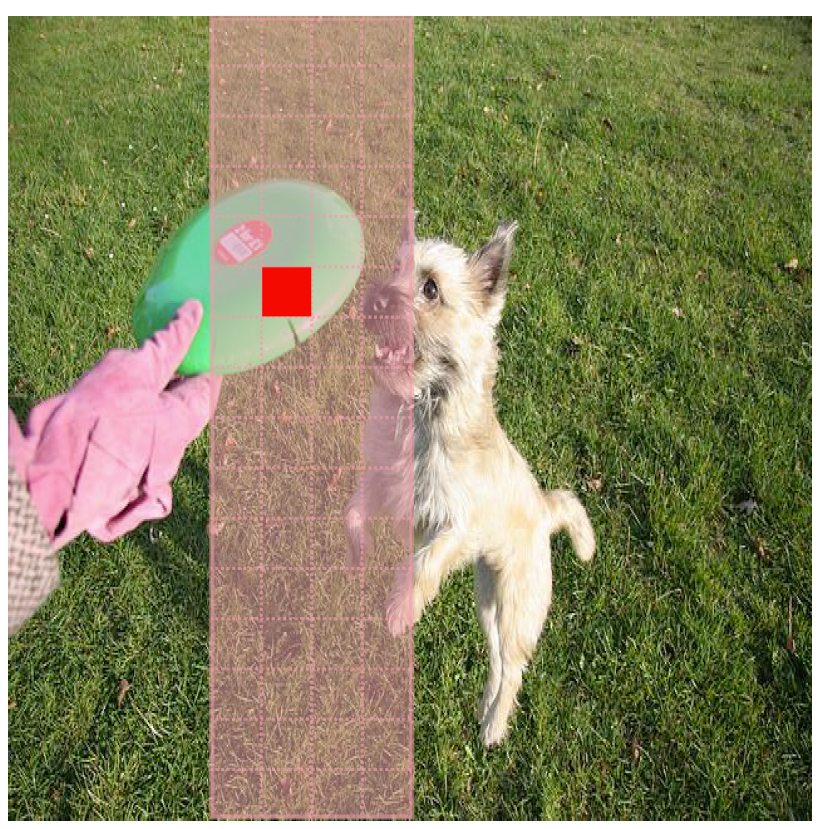
\includegraphics[width=\textwidth]{02-main/figures/ch2/ch2_yolo_05_attention_area_yolo2.png}
        \caption{Mécanisme d'attention vertical proposé dans YOLOv12}
        \label{fig:ch2_yolo_05_attention_area_yolo2}
    \end{subfigure}    
    \caption{Mécanismes d'attention \cite{tian_yolov12_2025}}
    \label{fig:ch2_yolo_mecanismes_attention}
\end{figure}

\paragraph{R-ELAN}
Les mécanismes d'attention rendent l'entraînement instable, particulièrement pour les gros modèles. La Figure \ref{fig:ch2_yolo_architecture_simplifiee} illustre l'évolution progressive des architectures de blocs dans la famille YOLO, depuis les premières approches jusqu'à la proposition YOLOv12.

CSPNet (Figure \ref{fig:ch2_yolo_06_architecture_csp}), utilisé dans YOLOv4/YOLOv5, est l'architecture fondatrice qui divise le flux de données en deux branches parallèles, permettant un meilleur gradient flow et réduisant les calculs redondants. Une branche traverse directement, l'autre passe par plusieurs blocs convolutionnels avant concaténation.

ELAN (Figure \ref{fig:ch2_yolo_07_architecture_elan}), utilisé dans YOLOv7, correspond aux Efficient Layer Aggregation Networks qui améliorent l'agrégation de caractéristiques en connectant explicitement différentes couches. Cette architecture permet une meilleure réutilisation des caractéristiques, mais souffre de problèmes de stabilité d'optimisation, particulièrement visibles dans les gros modèles.

$C_3K_2$ (Figure \ref{fig:ch2_yolo_08_architecture_c3k2}), utilisé dans YOLOv11, est l'évolution de GELAN (Generalized ELAN) qui simplifie l'architecture tout en conservant l'efficacité. $C_3K_2$ représente un cas particulier optimisé de GELAN, adopté pour réduire la latence dans YOLOv11.

R-ELAN (Figure \ref{fig:ch2_yolo_09_architecture_relan}) est l'architecture de bloc proposée dans YOLOv12. La contribution majeure des Residual Efficient Layer Aggregation Networks est l'ajout d'une connexion résiduelle avec facteur d'échelle (scaling) depuis l'entrée vers la sortie, inspirée des techniques de Vision Transformers. Cette modification résout les problèmes de convergence observés avec les mécanismes d'attention, particulièrement critiques pour les modèles YOLOv12-L et YOLOv12-X qui ne convergent pas sans cette stabilisation.


\begin{figure}[H]
    \centering
    \begin{subfigure}[b]{0.30\textwidth}
        \centering
        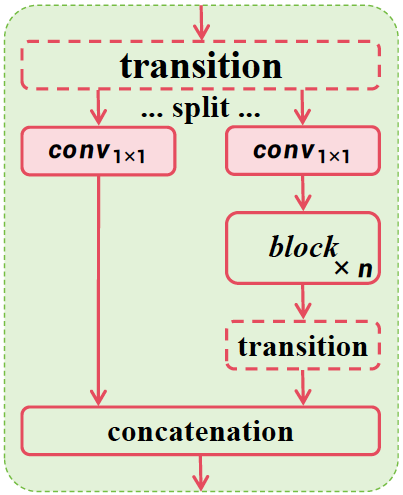
\includegraphics[width=\textwidth]{02-main/figures/ch2/ch2_yolo_06_architecture_csp.png}
        \caption{``CSPNet'' (YOLOv4/v5)}
        \label{fig:ch2_yolo_06_architecture_csp}
    \end{subfigure}
    \hfill
    \begin{subfigure}[b]{0.30\textwidth}
        \centering
        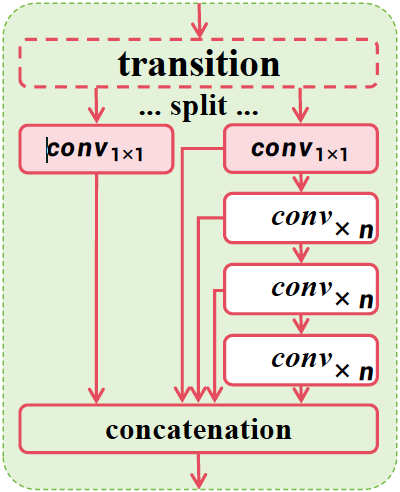
\includegraphics[width=\textwidth]{02-main/figures/ch2/ch2_yolo_07_architecture_elan.png}
        \caption{``ELAN'' (YOLOv7)}
        \label{fig:ch2_yolo_07_architecture_elan}
    \end{subfigure}
    \vspace{0.35cm}
    \begin{subfigure}[b]{0.45\textwidth}
        \centering
        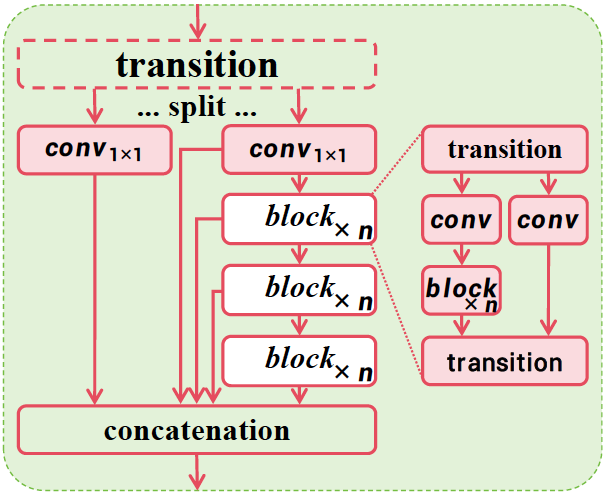
\includegraphics[width=\textwidth]{02-main/figures/ch2/ch2_yolo_08_architecture_c3k2.png}
        \caption{``$C_3K_2$'' (YOLOv11)}
        \label{fig:ch2_yolo_08_architecture_c3k2}
    \end{subfigure}
    \hfill
    \begin{subfigure}[b]{0.33\textwidth}
        \centering
        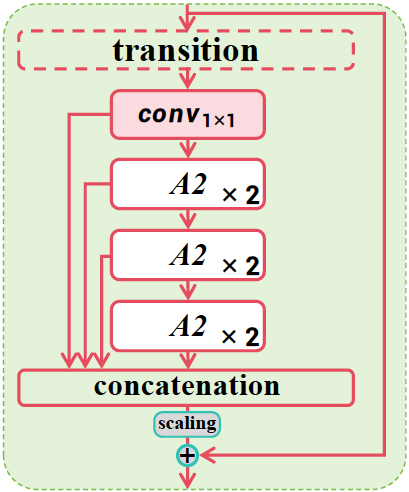
\includegraphics[width=\textwidth]{02-main/figures/ch2/ch2_yolo_09_architecture_relan.png}
        \caption{``R-ELAN'' (YOLOv12)}
        \label{fig:ch2_yolo_09_architecture_relan}
    \end{subfigure}
    \caption{Évolution architecturale des blocs utilisés dans YOLO \cite{tian_yolov12_2025}}
    \label{fig:ch2_yolo_architecture_simplifiee}
\end{figure}

\paragraph{Améliorations architecturales}
\citeauthor{tian_yolov12_2025} introduisent plusieurs optimisations architecturales cruciales pour adapter efficacement les mécanismes d'attention au contexte temps réel de YOLO.

FlashAttention \cite{dao_flashattention_2022} résout le problème fondamental d'accès mémoire des transformers. Traditionnellement, l'attention stocke des matrices intermédiaires volumineuses en mémoire GPU lente (HBM), créant un goulot d'étranglement. FlashAttention optimise ces accès mémoire, réduisant significativement la latence sans perte de précision.

La suppression de l'encodage positionnel simplifie drastiquement l'architecture par rapport aux Vision Transformers classiques. Cette décision contre-intuitive s'avère bénéfique, l'information spatiale est préservée grâce à un ``position perceiver'' (convolution séparable 7×7) appliqué aux valeurs d'attention, plus efficace que les encodages positionnels traditionnels.

La réduction du ratio MLP (Multilayer Perceptron) de 4.0 vers 1.2 rééquilibre la charge computationnelle entre les blocs d'attention et les réseaux feed-forward. Dans les Vision Transformers standards, le MLP consomme 75 \% des calculs ; YOLOv12 privilégie l'attention (plus bénéfique pour la détection) en réduisant la taille des MLP.


\subsubsection{Résultats principaux}
YOLOv12 établit un nouveau compromis vitesse-précision optimal qui démontre la viabilité des mécanismes d'attention pour la détection temps réel.

Les performances surpassent systématiquement les modèles existants. YOLOv12-N atteint 40.6\% mAP en 1.64 ms, dépassant YOLOv11-N de 1.2\% mAP à vitesse équivalente. Cette supériorité se maintient sur toutes les échelles de modèles.

L'efficacité computationnelle est remarquable face aux détecteurs bout-à-bout. YOLOv12-S (9.3 M paramètres) surpasse RT-DETR-R18 \cite{zhao_detrs_2024} (20 M paramètres) avec 42~\% de vitesse supplémentaire. Il utilise seulement 36~\% des calculs et 47~\% des paramètres.

Les cartes d'activation (Figure \ref{fig:ch2_yolo_10_perception}) révèlent une amélioration qualitative notable, avec des contours d'objets plus nets et une activation de premier plan plus précise comparé à YOLOv10/v11, illustrant concrètement les bénéfices des mécanismes d'attention optimisés.

\begin{figure}[H]
    \centering
    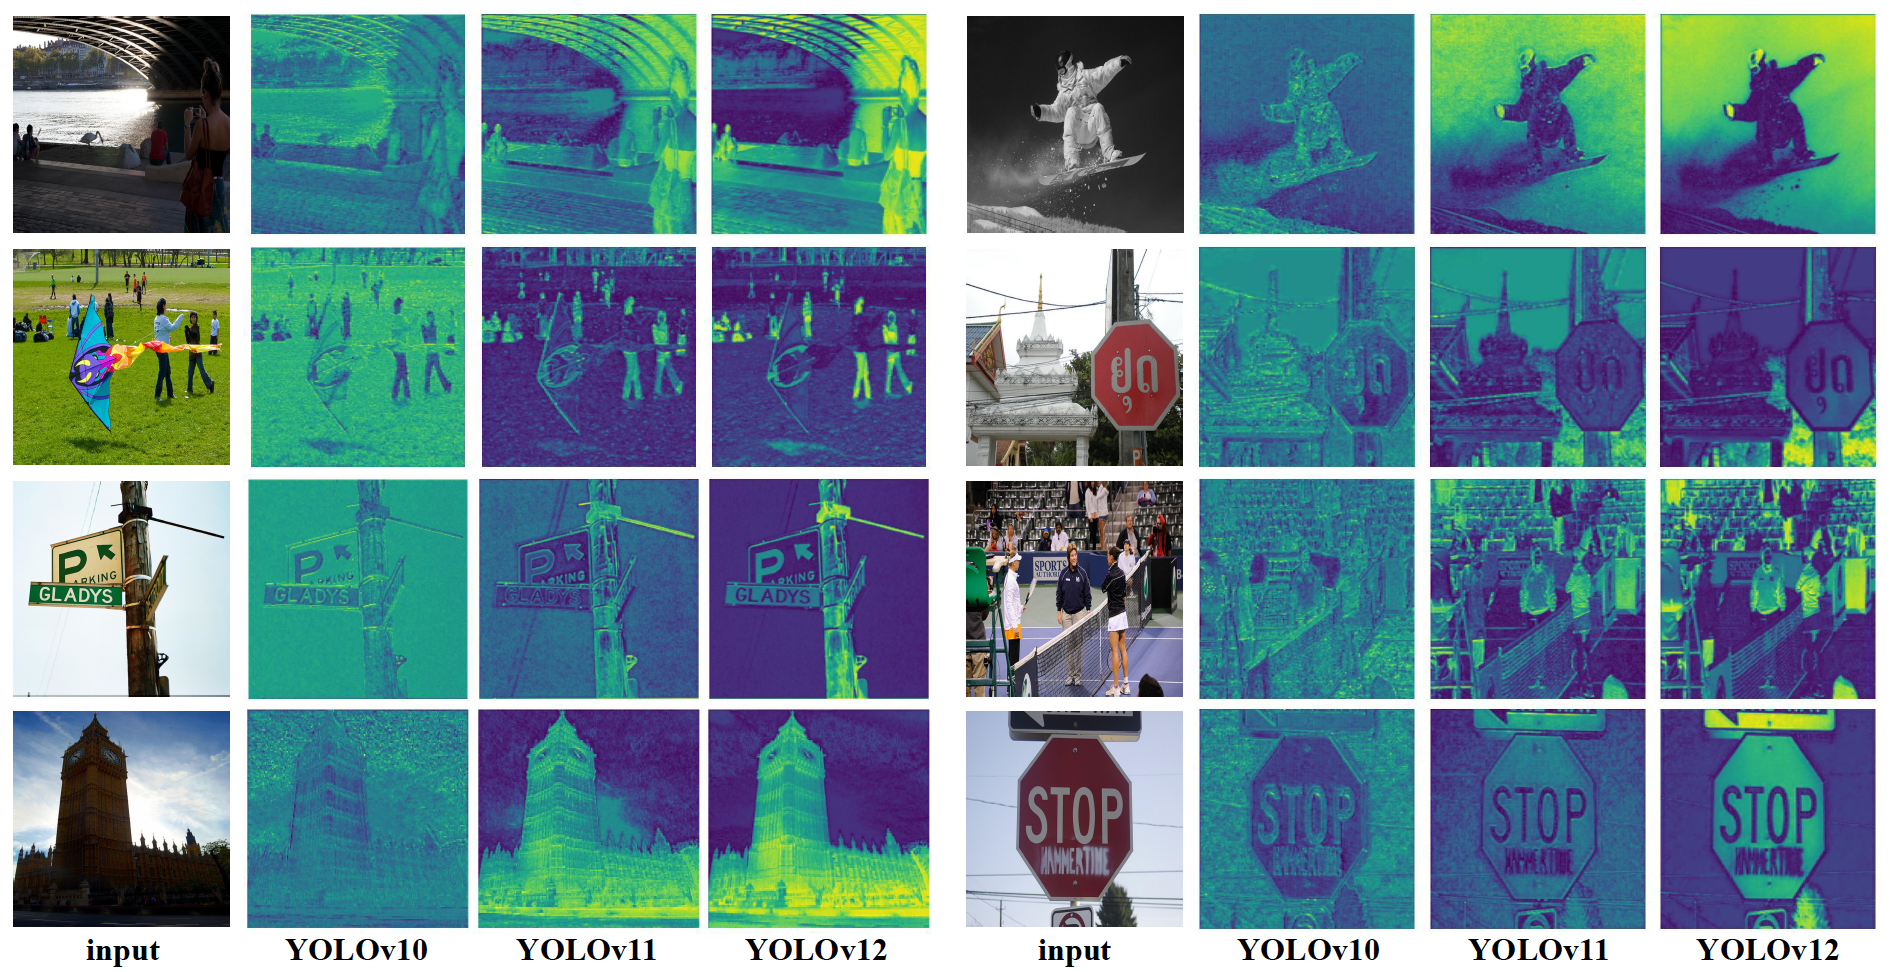
\includegraphics[width=1\linewidth]{02-main/figures/ch2/ch2_yolo_10_perception.png}
    \caption{Perception des objets dans YOLOv10, YOLOv11 et YOLOv12 \cite{tian_yolov12_2025}}
    \label{fig:ch2_yolo_10_perception}
\end{figure}

\subsubsection{Discussion et limites}
YOLOv12 représente une avancée majeure en démontrant que les mécanismes d'attention peuvent être rendus suffisamment efficaces pour la détection temps réel.

Si l'étude démontre théoriquement qu'il est possible de rendre l'attention suffisamment efficace pour la détection temps réel, l'impact pratique reste mitigé. \citeauthor{khanam_review_2025} \cite{khanam_review_2025} révèlent que YOLOv12 est à peine plus performant que ses prédécesseurs avec une architecture relativement complexe et plus gourmande en énergie.

La contrainte matérielle constitue une limitation majeure souvent sous-estimée. La dépendance exclusive à FlashAttention restreint l'utilisation aux GPU d'architecture Turing ou plus récente (RTX 20/30/40, A100, H100), excluant de facto une large base d'utilisateurs équipés de matériel plus ancien. Cette limitation est particulièrement problématique pour les applications industrielles où les cycles de renouvellement matériel sont longs. Cela affecte également les applications edge, dans lesquelles les ressources sont limitées et l'efficience énergétique du modèle est un paramètre critique.

\subsection{Segment}

\subsubsection{Contexte et objectifs}

\subsubsection{Données}

\subsubsection{Méthodologie}

\subsubsection{Résultats principaux}

\subsubsection{Discussion et limites}

\todo[inline]{Ajouter l'état de l'art pour les CNN choisies}
% -----------------------------------------------------------------------------
\subsection{?}

\subsubsection{Contexte et objectifs}

\subsubsection{Données}

\subsubsection{Méthodologie}

\subsubsection{Résultats principaux}

\subsubsection{Discussion et limites}
\todo[inline]{Effacer ça une fois l'état de l'art terminé}

% -----------------------------------------------------------------------------
% -----------------------------------------------------------------------------
\section{Datasets disponibles}
\label{sec:dataset_disponible}
\par{Quelques datasets de qualité sont disponibles actuellement. Ce chapitre va parcourir certains d'entre eux.}

% -----------------------------------------------------------------------------
\subsection{Roof Information Dataset for Computer Vision-Based Photovoltaic Potential Assessment (RID)}
\label{subsec:rid_roof_information_dataset}

\subsubsection{Contexte et objectifs}
\par{Malgré l'existence de dataset pour la segmentation des toitures des bâtiments ou la détection de panneaux solaires, aucun d'entre eux ne permet la segmentation sémantique complète des toitures et de leurs éléments. Dans ce contexte, \citeauthor{krapf_ridroof_2022} présentent le Roof Information Dataset (RID) \cite{krapf_ridroof_2022}, premier dataset public de segmentation de toitures et de leurs éléments.}

\subsubsection{Données}
\par{Le RID se compose d'images aériennes géo-référencées et d'annotations.}
\par{Les images sont des photos aériennes à haute résolution (environ 10 cm/pixel) centrées sur chaque bâtiment, téléchargées via l'API Google Maps Static pour la zone rurale de Wartenberg en Allemagne. Ces images sont géo-référencées au format GeoTIFF.}
\par{Les annotations sont des images rasterisées au format PNG}

\par{Les principaux chiffres-clés de ce dataset :}
\begin{itemize}
    \item 1880 bâtiments uniques répartis sur une zone de 1,5 km² (4,9 km² avec superposition)
    \item 4520 polygones de segments de toiture classés selon leur orientation géographique, en tout 5 classes :
    \begin{itemize}
        \item Nord, sud, est et ouest
        \item Toiture plate
    \end{itemize}
    \item 12359 polygones de superstructures répartis en 9 classes :
    \begin{itemize}
        \item Panneau PV
        \item Lucarne
        \item Fenêtre
        \item Échelle
        \item Cheminée
        \item Ombrage
        \item Arbre/végétation
        \item Fond d'image (background)
        \item Inconnu
    \end{itemize}
\end{itemize}
\par{Les annotations sont fournies en deux versions différentes. La version initiale a été réalisées par cinq annotateurs. Ensuite deux annotateurs supplémentaires ont corrigés et compléter les annotations initiales. La Figure \ref{fig:rid_dataset_image_sample} représente avec une image d'exemple les différences entre les annotations.}

\begin{figure}[H]
    \makebox[\textwidth][c]{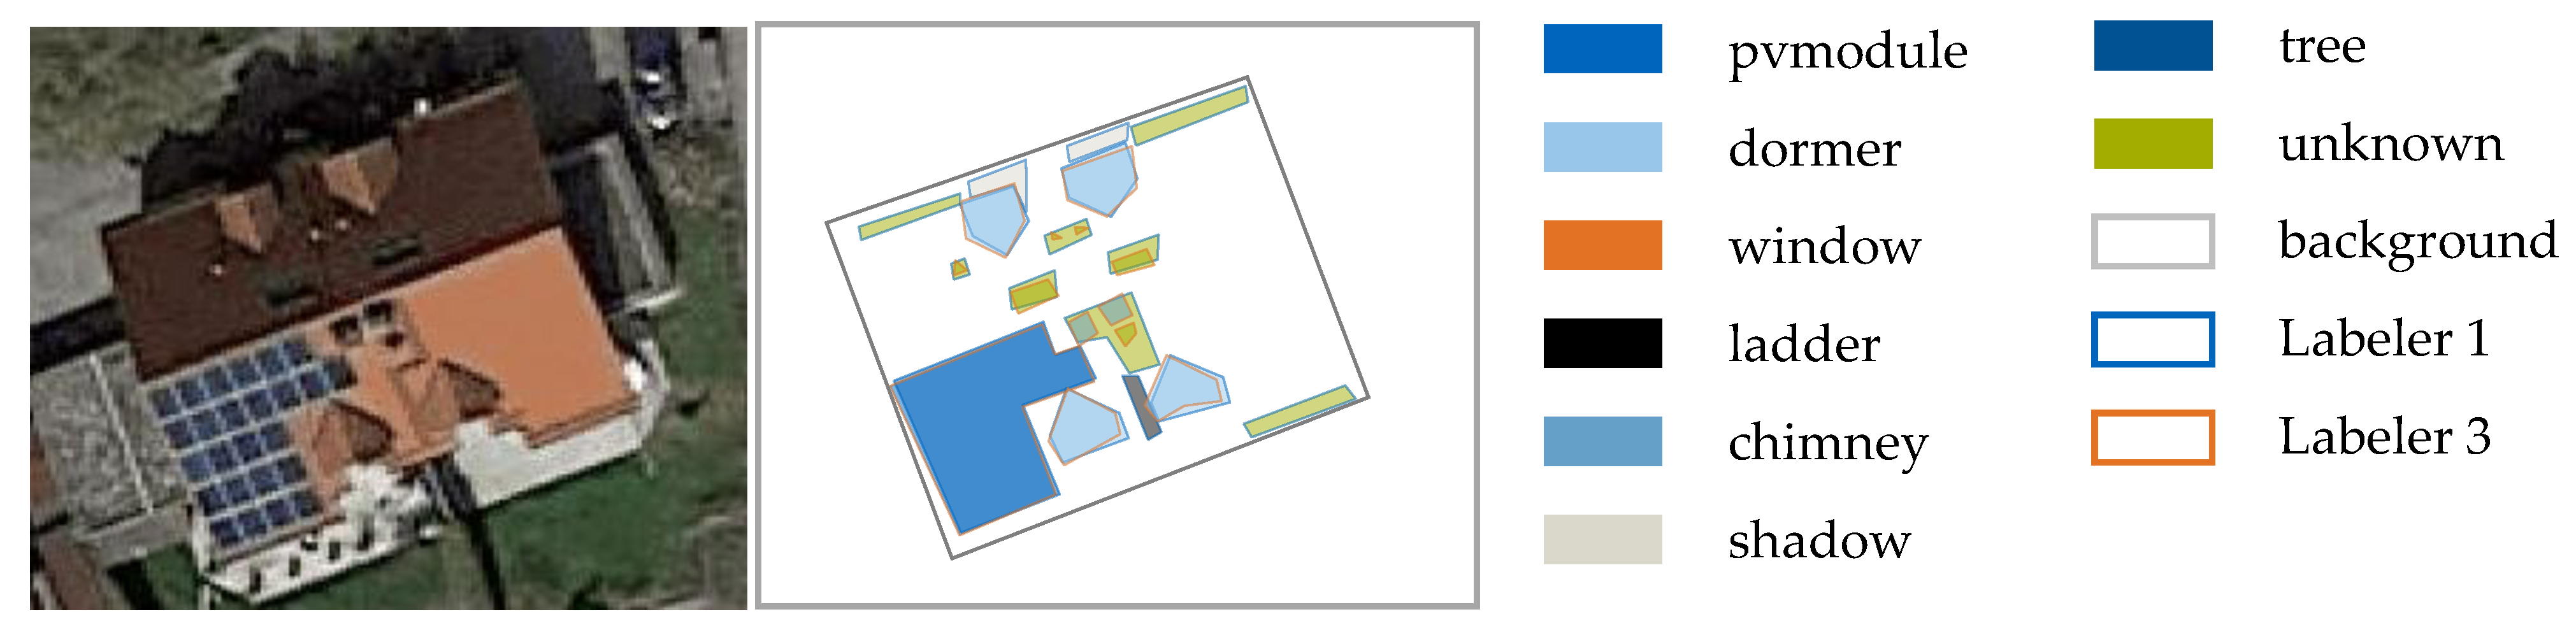
\includegraphics[width=1.15\textwidth]{02-main//figures/ch2/rid_dataset_image_sample.png}}
    \caption{Exemple d'image du dataset, ainsi que les différentes annotations des annotateurs \cite{krapf_rid_2021}}
    \label{fig:rid_dataset_image_sample}
\end{figure}

\par{La Figure \ref{fig:rid_dataset_distribution_classes} représente la distribution des éléments de toiture par classe.}
\begin{figure}[H]
    \centering
    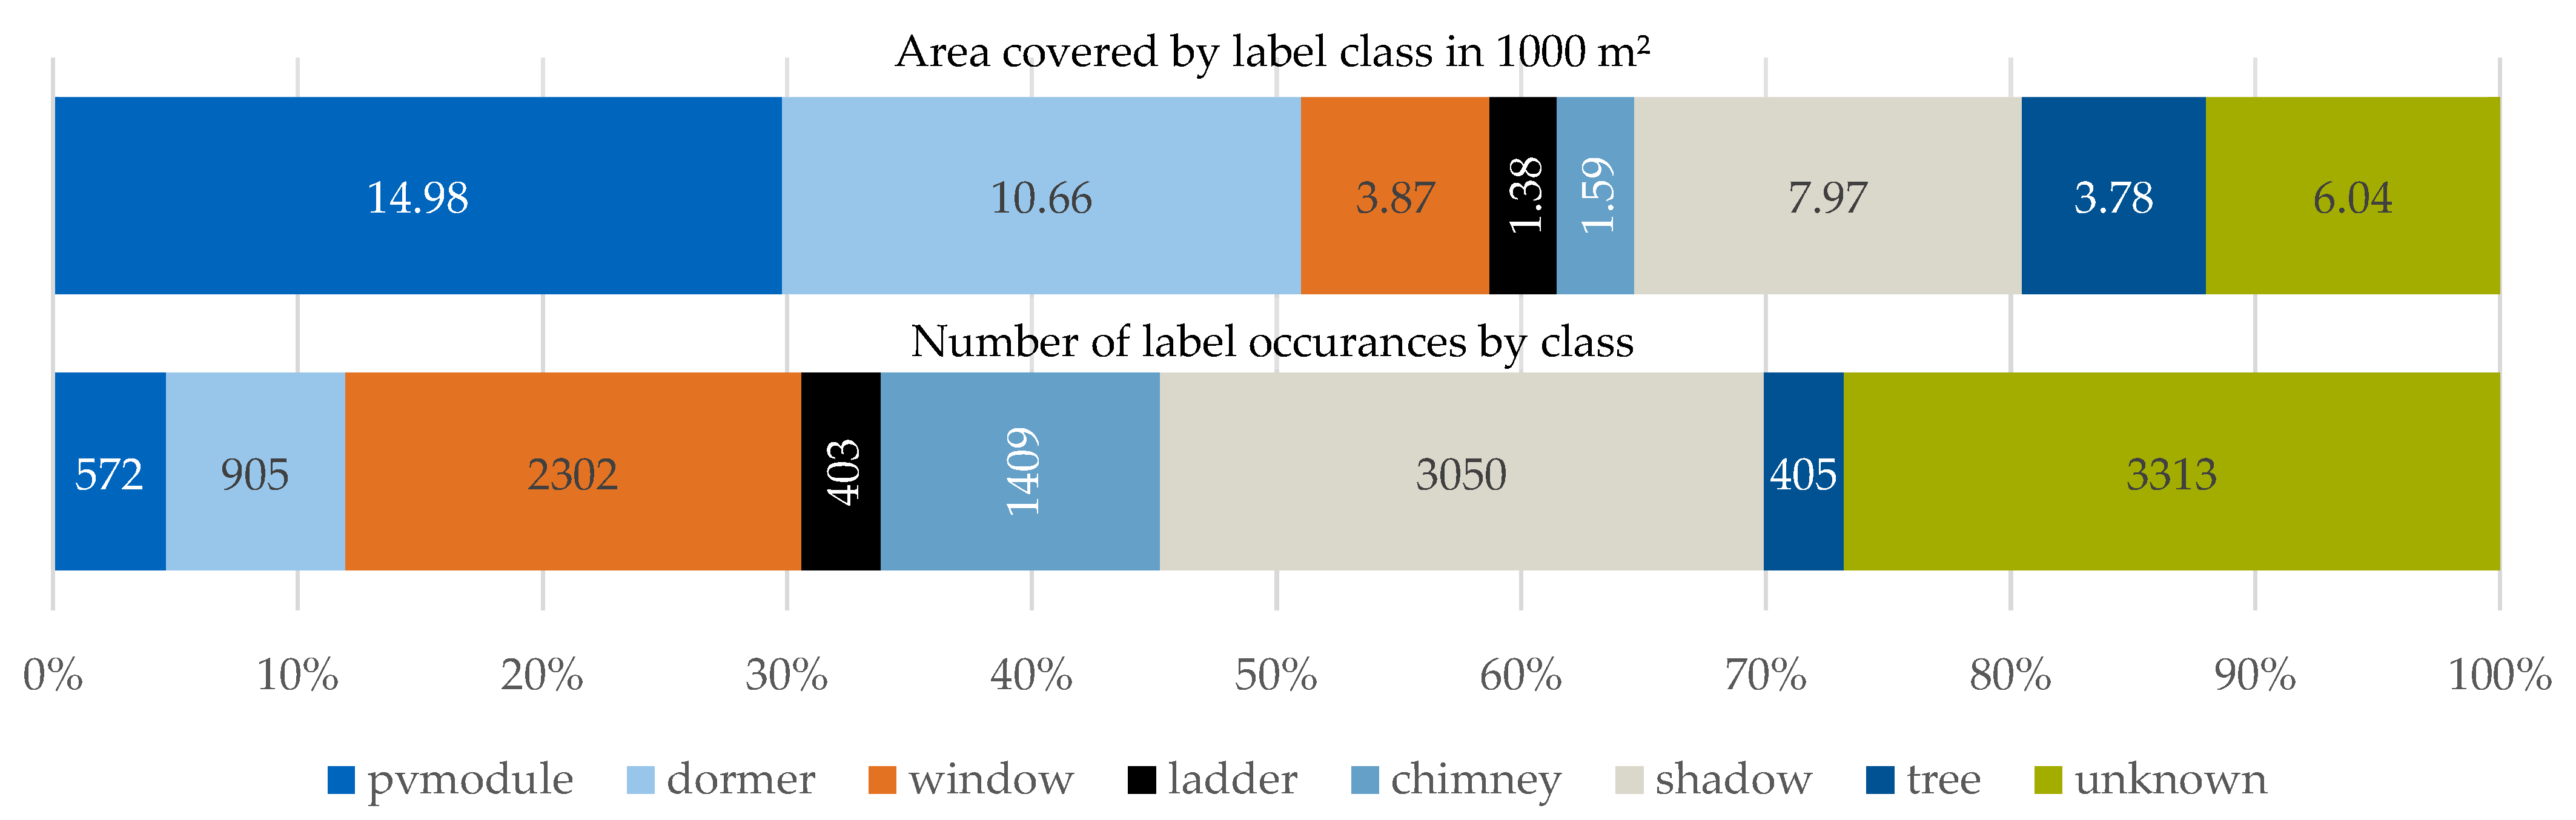
\includegraphics[width=1\linewidth]{02-main//figures/ch2/rid_dataset_distribution_classes.png}
    \caption{Distribution des classes dans le dataset des éléments de toiture \cite{krapf_ridroof_2022}}
    \label{fig:rid_dataset_distribution_classes}
\end{figure}
\par{Le dataset est disponible en ligne \cite{krapf_rid_2021} ainsi que le code \cite{krapf_tumftmrid_2025}.}

\subsubsection{Méthodologie}
\par{Le processus de création du dataset s'est déroulé en plusieurs phases :}
\begin{enumerate}
    \item Sélection de la zone d'étude :
    \begin{itemize}
        \item Zone rurale de Wartenberg (Munich) choisie pour offrir des images de qualité variable (contraste, ombres, distorsions) afin d'améliorer la capacité des modèles à s'adapter à des conditions variables
    \end{itemize}
    \item Acquisition des données :
    \begin{itemize}
        \item Téléchargement d'images aériennes via l'API Google Maps
        \item Résolution d'environ 10 cm/pixel, suffisante pour identifier les petites éléments présents sur les toitures comme les cheminées
    \end{itemize}
    \item Processus d'annotation initial :
    \begin{itemize}
        \item Développement d'un outil d'annotation personnalisé permettant de dessiner des polygones sur l'interface Google Maps Dynamic API
        \item Annotation par cinq membres universitaires suivant un ensemble de règles prédéfini
        \item Deux tâches d'annotation distinctes : segments de toiture (classes N, S, W, O, plat) et les éléments présents sur les toitures.
    \end{itemize}
    \item Évaluation de la qualité d'annotation :
    \begin{itemize}
        \item Expérience d'annotation comparative sur 26 bâtiments sélectionnés pour contenir au moins 15 occurrences de chaque classe de superstructure
        \item Analyse de l'accord entre annotateurs pour identifier les classes les plus difficiles à annoter
    \end{itemize}
    \item Processus de révision :
    \begin{itemize}
        \item Utilisation de l'outil CVAT (Computer Vision Annotation Tool) permettant un zoom plus important
        \item Révision par deux annotateurs n'ayant pas participé à l'annotation initiale pour limiter les biais
        \item Attention particulière aux classes ayant montré un faible accord inter-annotateurs
    \end{itemize}
    \item Répartition manuelle des données en dataset d'entraînement, validation et test :
    \begin{itemize}
        \item Division géographique (et non aléatoire) pour éviter le chevauchement entre ensembles d'entraînement et de test
        \item Création de cinq configurations de partitionnement différentes pour la validation croisée (cross-validation)
    \end{itemize}

    \item Application à l'estimation du potentiel photovoltaïque :
    \begin{itemize}
        \item Entraînement de réseaux de neurones (U-Net et Panoptic FPN) pour la détection des éléments de toiture
        \item Conversion des masques de segmentation en géométries vectorielles
        \item Calcul du potentiel photovoltaïque en tenant compte des éléments de toiture
    \end{itemize}
\end{enumerate}

\subsubsection{Résultats principaux}
L'article présente plusieurs catégories de résultats :
\begin{enumerate}
    \item Qualité des annotations :
    \begin{itemize}
        \item Forte variabilité de l'accord inter-annotateurs (IoU) selon les classes
        \item Classes avec bon accord : lucarnes (0,70) et panneaux solaires (0,68)
        \item Classes problématiques : objets inconnus (0,15), échelles (0,22)
        \item IoU moyen global de 0,48 pour l'annotation initiale et performance plus élevée après révision
    \end{itemize}
    \item Performances des réseaux de neurones :
    \begin{itemize}
        \item U-Net et Panoptic FPN entraînés et testés sur les deux versions du dataset
        \item Meilleure performance : U-Net avec IoU moyen de 0,42-0,44 sur le jeu de test initial
        \item Performance améliorée à 0,45-0,46 sur les annotations révisées
        \item Réseaux capables de compenser partiellement les incohérences d'annotation
        \item Détection performante des panneaux solaires (IoU 0,69) et lucarnes (IoU 0,60)
    \end{itemize}
    \item Impact sur l'évaluation du potentiel photovoltaïque :
    \begin{itemize}
        \item La prise en compte des éléments de toiture réduit significativement le potentiel PV estimé
        \item Réduction de 20,5\% avec annotations manuelles et 15,0\% avec prédictions du réseau
        \item Avec une approche de placement réaliste des modules, réduction de 31,1\%
        \item Impact très variable selon les toitures : de moins de 5\% pour 39\% des toits à plus de 70\% pour 10\% des toits
        \item L'exclusion des segments déjà équipés de panneaux solaires réduit le potentiel de 29,5\%
    \end{itemize}
\end{enumerate}
\par{Ces résultats démontrent l'importance de considérer les éléments de toiture dans l'évaluation du potentiel solaire des toitures et valident l'approche par apprentissage profond sur images aériennes comme alternative viable aux méthodes basées sur \gls{lidar}, malgré les défis liés à la qualité des annotations.}

\subsubsection{Discussion et limites}
\par{Le dataset se concentre sur une zone rurale allemande et ne représente pas adéquatement d'autres styles architecturaux. Comme indiqué dans la section \ref{subsec:solar_net_plus} qui fait référence a un article postérieur du même auteur, le dataset n'est pas adapté au milieu urbain de Bruxelles. Les classes sont trop spécifiques au rural allemand, dans le cas de Bruxelles, il manque les classes pour des éléments typiquement urbains tel que les ventilation/climatisation.}
\par{Il y a une forte disproportion entre les classes d'éléments de toiture, avec certaines classes très peu représentées et d'autres classes étant dans toutes les images (cas classe "background").}
\par{L'article s'intéresse aussi à la variabilité de la qualité d'annotation. Les annotateurs ne sont pas toujours d'accord sur les annotations (polygone) et les classes. La qualité des annotations a un impact sur la performance des modèles. Les variations dans les annotations sont aussi en partie dues a la résolution des images, celle-ci peux être insuffisante pour clairement identifier et annoter les petits objets.}
\par{Les résultats des deux modèles sont encourageants, mais doivent être pris comme point de départ pour améliorer la qualité du dataset.}

% -----------------------------------------------------------------------------
\subsection{Autres dataset}

\par{Le dataset de la section précédente est le seul disponible en ligne qui permet de faire de la segmentation sémantique des éléments de toiture. La plupart des articles ne partagent pas leur dataset, plusieurs hypothèses sont possible:}
\begin{itemize}
    \item Contraintes contractuelles avec les fournisseurs d'images qui limitent leur diffusion
    \item Les datasets annotés représentent un investissement considérable en temps et ressources, constituant un capital intellectuel précieux pour de futures publications ou demandes de financement.    
    \item Difficultés liées au stockage et à la distribution de volumes importants de données géospatiales, ainsi qu'à la maintenance d'une infrastructure adéquate pour supporter l'accès externe.
    \item L'effort nécessaire pour documenter, nettoyer et préparer un dataset à usage public dépasse souvent les ressources disponibles ou allouées dans le cadre du projet initial.
    \item Manque de reconnaissance académique formelle pour le partage de données comparativement aux publications d'articles, et parfois politiques institutionnelles restrictives concernant la propriété intellectuelle.
\end{itemize}
\par{La section suivante décrit les datasets disponibles pour les panneaux solaire PV, cela reste tout de même en lien avec l'identification des éléments de toiture.}

\subsubsection{Datasets dédiés aux panneaux solaires PV}
\par{Plusieurs datasets spécifiques à la détection et segmentation des panneaux solaires photovoltaïques sont disponibles dans la littérature scientifique. La plateforme Roboflow Universe \cite{roboflow_roboflow_nodate}, qui héberge plus de 500'000 datasets, propose une dizaine de datasets dédiés à la segmentation sémantique ou à la classification des panneaux solaires. Cependant, ces datasets présentent généralement des limitations importantes: nombre restreint d'images et annotations de qualité variable.}
\par{Parmi les datasets plus significatifs, celui publié par \citeauthor{kasmi_crowdsourced_2023} \cite{kasmi_crowdsourced_2023, kasmi_crowdsourced_2022} se distingue par son approche collaborative. Son objectif principal est la détection binaire de panneaux solaires PV dans des images satellite. Ce dataset a la particularité d'avoir été prévu pour être enrichi continuellement grâce à un système de labellisation participatif accessible via GitHub \cite{gabrielkasmi_gabrielkasmibdappv_2025}. À ce jour, il recense environ 28'000 installations photovoltaïques sur plus de 33'000 images satellite. Ses sources de données sont l'IGN (Institut national de l'information géographique et forestière) ainsi que Google.}
\par{Un autre dataset notable a été publié par \citeauthor{thebault_comprehensive_2025} \cite{thebault_comprehensive_2025}. Baptisé FRPV \cite{thebault_frpv_2025}, ce dataset a été utilisé pour évaluer le potentiel solaire photovoltaïque en France. Il combine des images provenant de l'IGN et de Google Maps, pour un total de 23'709 images contenant des installations photovoltaïques et 45'418 images sans installation PV, offrant ainsi un corpus équilibré pour l'entraînement de modèles de classification.}

% -----------------------------------------------------------------------------
% -----------------------------------------------------------------------------
\section{Solutions commerciales existantes}
\par{Quelques entreprises offrent des solutions pour réaliser un cadastre solaire sur la base de leur données. Dans tous les cas leur méthodologie ou les données utilisées ne sont pas disponible.}
\par{Solargis \cite{solargis_regional_nodate} est un société spécialisée dans le solaire. Cette entreprise offre diverses solutions pour planifier toutes les phases de chantier, depuis la modélisation d'un site jusqu'au suivi et à l'optimisation des performances des panneaux solaires en phase d'exploitation. Ils offrent aussi la prestation de création d'un cadastre solaire pour une région.}
\par{L'entreprise Picterra \cite{picterra_infrastructure_nodate} offre des solutions pour l'utilisation de machine learning sur des données géomatiques. Entre autres, ils proposent l'estimation du potentiel solaire d'une région. Une autre entreprise suisse, Urbio, \cite{urbio_urbio_nodate} offre aussi des prestations similaires à Picterra mais plus axées sur la planification énergétique.}
\par{Google Projet Sunroof \cite{google_project_nodate} exploite les données de Google pour évaluer le potentiel solaire des différentes régions. Cette plateforme propose également quelques conseils pour l'obtention de subventions. Bien que les données générées soient accessibles au public, Google ne les produit que pour les municipalités et régions qui souscrivent à leurs services. Cette solution est actuellement limitée aux USA.}

% -----------------------------------------------------------------------------
% -----------------------------------------------------------------------------
\section{Synthèse}

\par{L'analyse de l'état de l'art révèle trois approches principales pour l'évaluation du potentiel solaire des toitures, chacune présentant des avantages et limitations spécifiques.}

\par{Les méthodes traditionnelles basées sur les données \gls{lidar} et cadastrales, illustrées par les cadastres solaires genevois et suisse (ToitSolaire), offrent une couverture territoriale complète et disposent des validations nécessaires du point de vue académique. Cependant, elles souffrent des mêmes limitations, il n'y pas actuellement de cartographie précise des toitures. Par conséquent, sans la prise en compte de tous les obstacles présents sur les toitures, le potentiel solaire sera surestimé.}

\par{Les approches par machine learning supervisé, exemplifiées par les travaux de \citeauthor{castello_quantification_2021} et \citeauthor{li_deep_2024}, démontrent une capacité prometteuse à identifier automatiquement les surfaces disponibles et les obstacles sur les toitures. Ces méthodes atteignent des performances satisfaisantes (IoU de 64\% pour \citeauthor{castello_quantification_2021}, \%RMSE de 19,92\% pour SolarNet+) mais restent limitées par la disponibilité et la qualité des données d'entraînement annotées.}

\par{L'étude du \acrshort{stdl} illustre la complémentarité des différentes sources de données (\gls{lidar}, orthophotos, données vectorielles) et techniques (classification, segmentation). La combinaison par concaténation des résultats de segmentation \gls{lidar} et d'images atteint un F1-score de 0.79 avec un recall de 0.94, démontrant l'intérêt d'approches hybrides.}

\par{Concernant les données disponibles, le dataset RID constitue actuellement la seule ressource publique permettant la segmentation sémantique complète des éléments de toiture. Cependant, sa limitation à un contexte rural allemand restreint sa généralisation à d'autres environnements urbains.}

\par{Les limites identifiées pointent vers la nécessité de combiner les approches traditionnelles éprouvées avec les techniques de machine learning, condition nécessaire au développement de datasets couvrant une plus grande diversité architecturale. L'exploitation conjointe d'images aériennes et d'informations géomatiques plus poussée s'impose comme l'approche la plus prometteuse pour obtenir un cadastre solaire fiable.}
\chapter{Design}
\label{chap:design}

\lipsum[1]

% \minitoc

\newpage

% -----------------------------------------------------------------------------
\section{Short lists}

\blindtext

\blindlist{enumerate}

\blindtext

\blindtext

\blindlist{itemize}

\blindtext

\blinddescription

% -----------------------------------------------------------------------------
\section{Long lists}

\blindtext

\Blindlist{enumerate}

\blindtext

\Blindlist{itemize}

\blindtext

\Blinddescription

% -----------------------------------------------------------------------------
\section{Multi-level lists}

\blindtext

\blindlistlist[3]{itemize}

\blindtext

\blindlistlist[3]{enumerate}

% -----------------------------------------------------------------------------
\section{Conclusion}

\lipsum[6-7]

\chapter{Évaluation, validation et analyse}
\label{chap:eval_valid_modele}
Ce chapitre présente l'évaluation des modèles de segmentation développés pour identifier les espaces libres sur les toitures du canton de Genève. L'objectif est d'analyser les performances de 93 configurations sur un dataset de test indépendant pour déterminer les architectures les plus adaptées à un déploiement opérationnel.

L'évaluation suit trois axes principaux : l'analyse quantitative des performances avec plusieurs métriques (IoU, mAP, F1-score), l'étude du rapport entre performance et complexité des modèles, et la validation qualitative sur des cas réels incluant un quartier absent des données d'entraînement. Cette approche permet de sélectionner la meilleure configuration et d'identifier les améliorations nécessaires pour renforcer la robustesse du système.
\localtableofcontents

\newpage

% -----------------------------------------------------------------------------
\section{Évaluation sur le dataset de test}

\subsection{Protocole d'évaluation}

L'évaluation des modèles a été réalisée sur un dataset de test indépendant composé de 89 images représentatives du canton de Genève. Cette évaluation porte sur 93 configurations distinctes, comprenant 89 modèles issus de Segmentation Models PyTorch (SMP) et 4 variantes de YOLOv12. Pour garantir la robustesse des résultats, chaque configuration a été entraînée selon une validation croisée à 5 folds, permettant d'obtenir des performances moyennées et des écarts-types significatifs.

Chaque fold de l'ensemble des modèles testés a fait l'objet d'au minimum 3 entraînements. Pour l'évaluation finale, seul l'entraînement ayant obtenu le meilleur IoU parmi tous ceux réalisés pour chaque fold a été conservé. Chaque modèle dispose de 5 folds, les résultats présentés sont la moyenne des performances sur ces 5 folds.

Pour des raisons pratiques de visualisation, YOLO est intégré dans les graphiques en tant que décodeur et ses différentes variantes en tant qu'encodeurs. Cette représentation vise uniquement à faciliter la comparaison des résultats, car YOLOv12 constitue un modèle complet qui ne peut pas être divisé en composants encodeur-décodeur interchangeables comme les modèles SMP.

\subsubsection{Métriques d'évaluation}

Les performances des modèles ont été évaluées selon plusieurs métriques complémentaires :

\begin{itemize}
    \item IoU (Intersection over Union) : métrique principale mesurant le recouvrement entre les prédictions et les annotations de référence
    \item mAP@k : mean average precision à différents seuils d'IoU (50\%, 75\%, 95\%)
    \item F1-score : moyenne harmonique entre precision et recall
    \item Métriques classiques : accuracy, precision et recall
\end{itemize}

Les aspects computationnels ont également été mesurés :
\begin{itemize}
    \item Temps d'entraînement total pour les 5 fold
    \item Nombre de paramètres du modèle (en millions)
\end{itemize}

\subsection{Vue d'ensemble des performances}

\subsubsection{Distribution globale des résultats}

Le Tableau \ref{tab:vue_ensemble_metrique_moyennes} présente les statistiques de base des 93 modèles évalués. Ils présentent des IoU s'échelonnant de 0,619 à 0,741, avec une moyenne de 0,708 et un écart-type de 0,024. Cette faible dispersion témoigne de la qualité générale des architectures modernes de segmentation sur cette tâche spécifique.

\begin{table}[H]
    \centering
    \begin{tabular}{@{}lrrrr@{}}
    \toprule
    \textbf{Métrique} & \textbf{Moyenne} & \textbf{Médiane} & \textbf{Minimum} & \textbf{Maximum} \\
    \midrule
    IoU & 0.708 $\pm$ 0.024 & 0.711 & 0.619 & 0.741 \\
    F1 Score & 0.775 $\pm$ 0.048 & 0.787 & 0.544 & 0.810 \\
    mAP@0.5 & 0.818 $\pm$ 0.056 & 0.834 & 0.556 & 0.854 \\
    mAP@0.75 & 0.592 $\pm$ 0.073 & 0.609 & 0.347 & 0.694 \\
    mAP@0.95 & 0.109 $\pm$ 0.036 & 0.110 & 0.029 & 0.191 \\
    Accuracy & 0.946 $\pm$ 0.101 & 0.968 & 0.451 & 0.976 \\
    Recall & 0.816 $\pm$ 0.043 & 0.823 & 0.616 & 0.872 \\
    Precision & 0.773 $\pm$ 0.043 & 0.786 & 0.577 & 0.812 \\
    Temps d'entraînement (h.) & 20.266 $\pm$ 10.698 & 19.557 & 1.792 & 48.268 \\
    \bottomrule
    \end{tabular}
    \caption{Statistiques générales des modèles évalués sur le dataset de test}
    \label{tab:vue_ensemble_metrique_moyennes}
\end{table}

La Figure~\ref{fig:heatmap_iou} présente une vue synthétique des performances pour chaque combinaison encodeur-décodeur.

\begin{figure}[H]
    \centering
    \makebox[\textwidth][c]{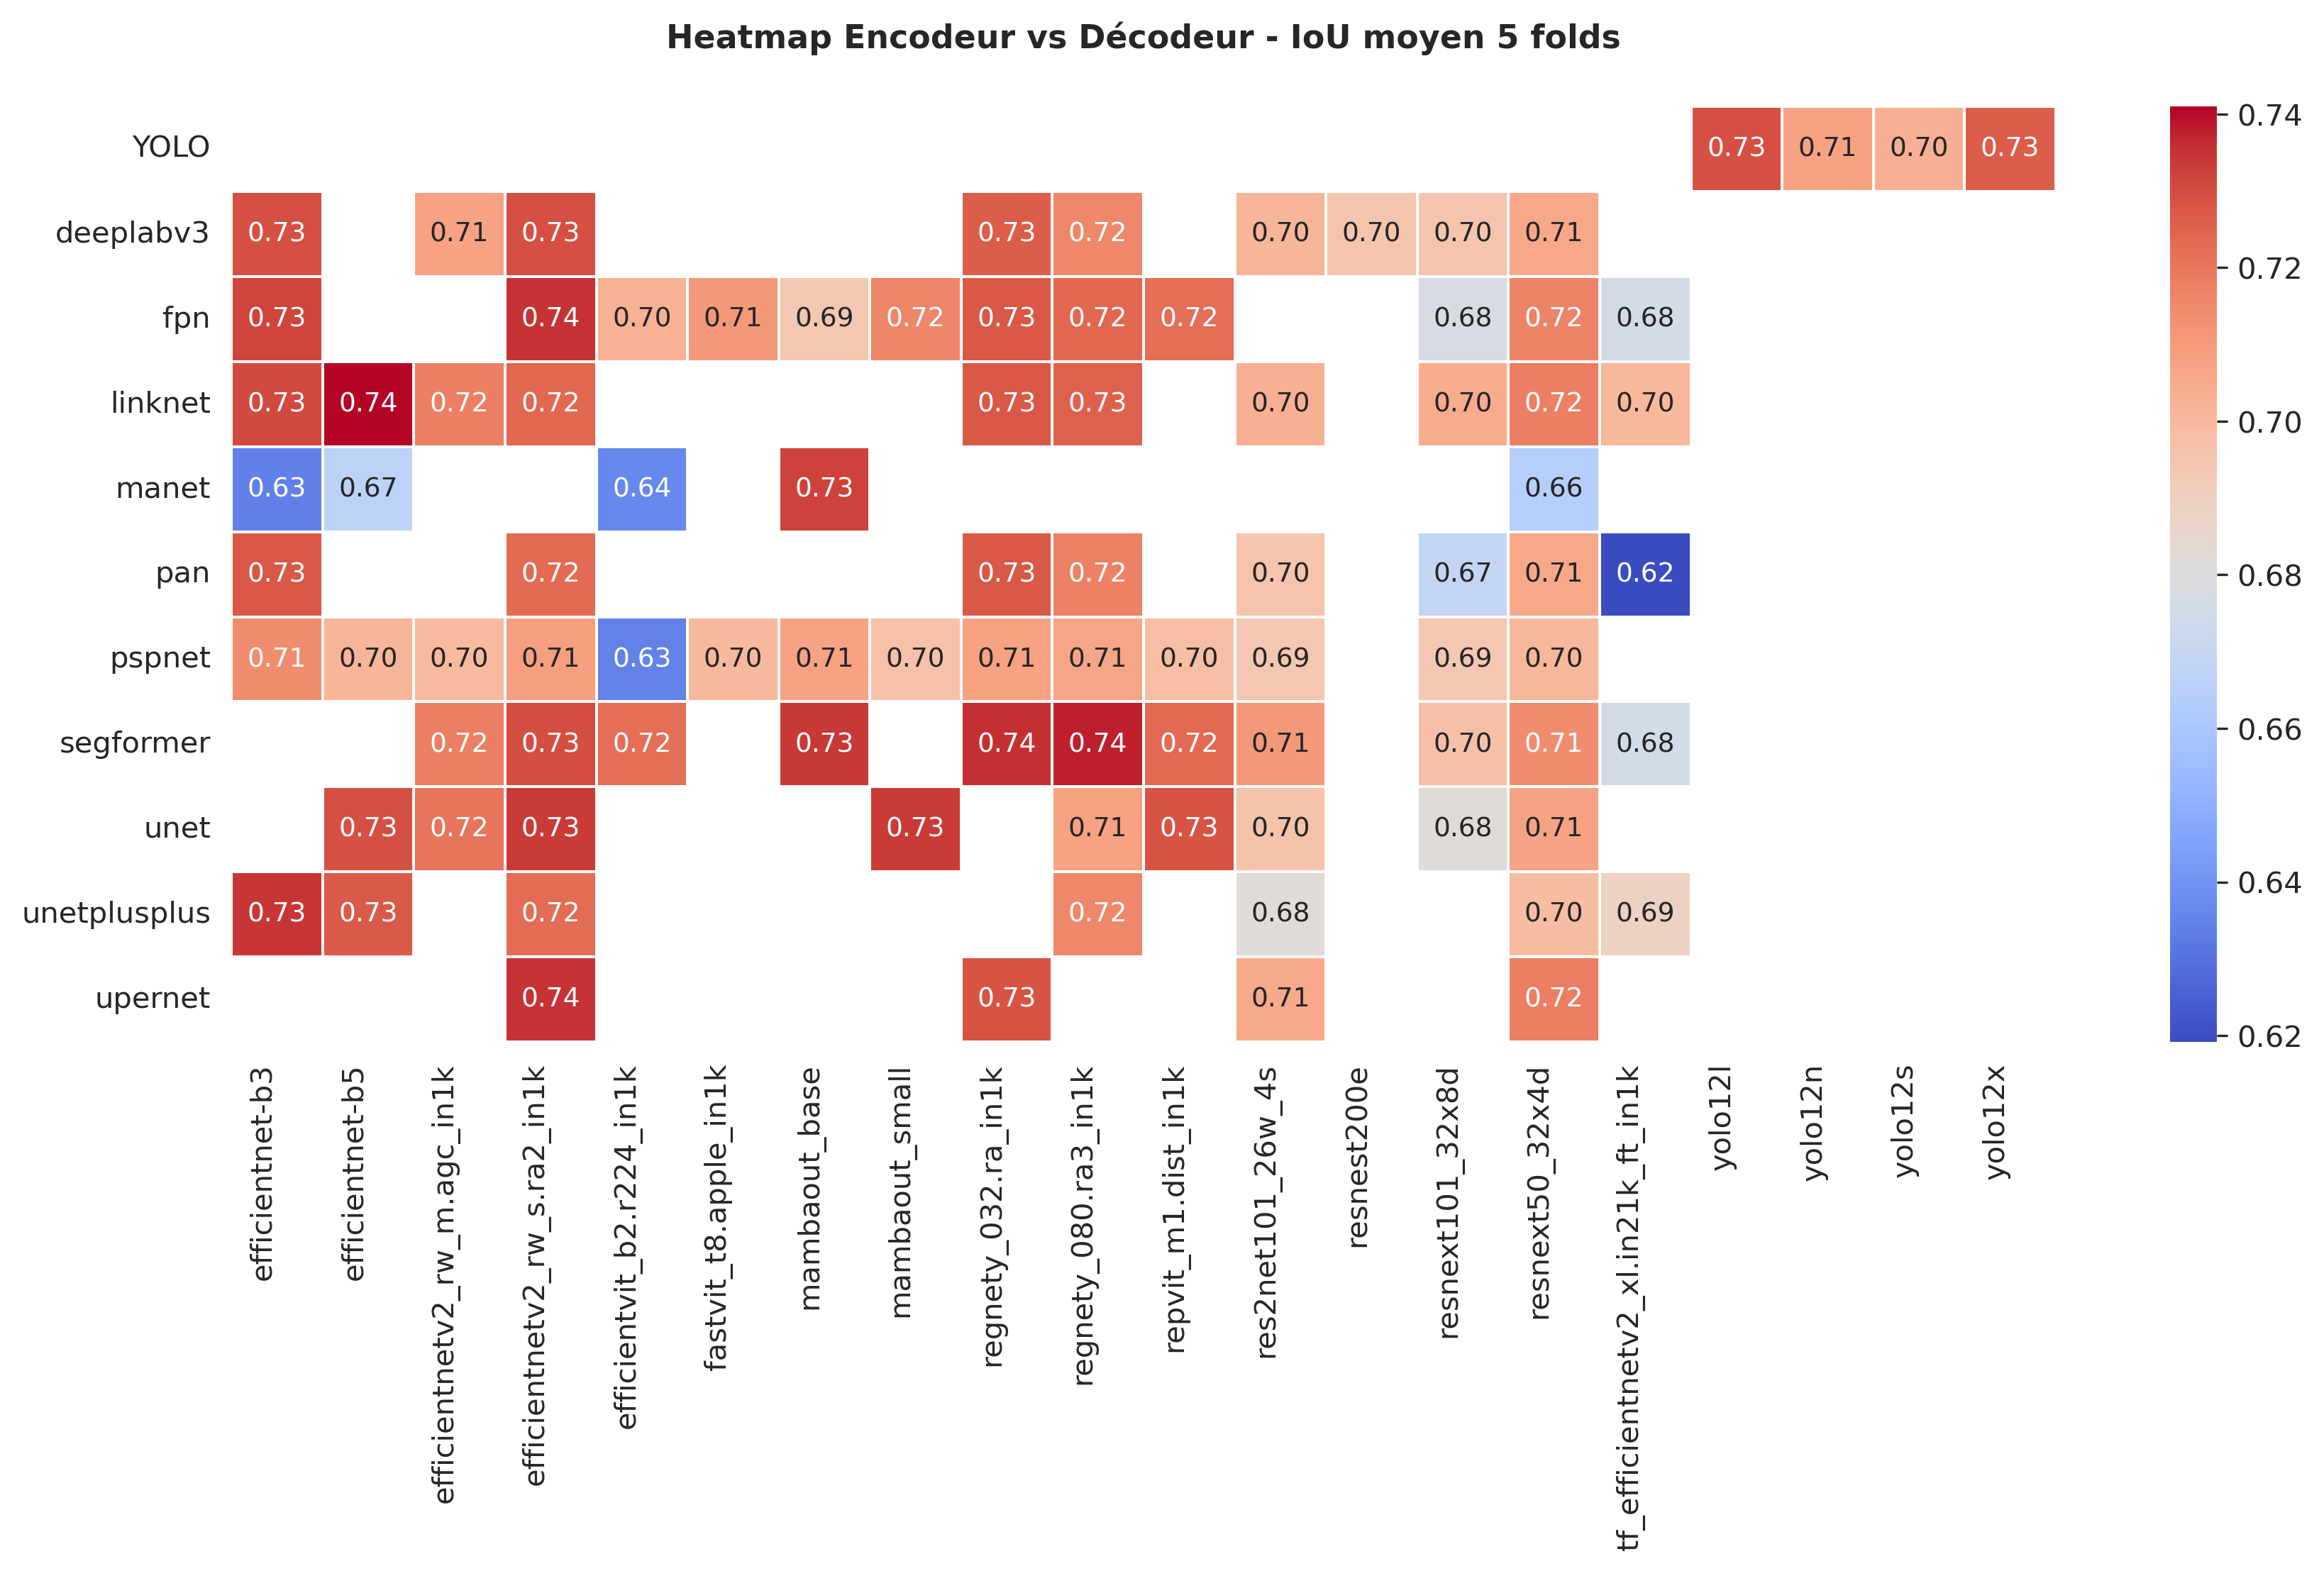
\includegraphics[width=1.45\textwidth]{02-main//figures/ch4/ch4_01_architecture_backbone_heatmap_01_eval_test_iou_mean.png}}
    \caption{Heatmap IoU par combinaison encodeur-décodeur}
    \label{fig:heatmap_iou}
\end{figure}

Certaines combinaisons d'encodeur et de décodeur présentent des cases vides car elles ont échoué lors de l'entraînement. L'échec peut être dû à de très mauvaises performances avec un IoU inférieur à 0,2, ce qui indique que le modèle n'a pas réussi à apprendre les caractéristiques de la tâche. D'autres échecs résultent d'incompatibilités entre les encodeurs et décodeurs, certains d'entre eux nécessitant des réglages très spécifiques qui n'ont pas été explorés par manque de temps.

Par exemple, YOLOv12m obtient un IoU de 0,11, ce qui est relativement surprenant comparé aux performances des autres modèles de la famille YOLOv12.

Ces modèles semblent tous présenter des résultats exceptionnels à première vue, mais il est important de visualiser le F1-score (Figure \ref{fig:ch4_01_architecture_backbone_heatmap_08_eval_test_f1_score_mean}) pour mieux comprendre la qualité des prédictions. Le F1-score constitue une métrique plus robuste car elle prend en compte à la fois la precision et le rappel, ce qui s'avère crucial pour les tâches de segmentation où les faux positifs et les faux négatifs peuvent avoir un impact significatif.

\begin{figure}[H]
    \centering
    \makebox[\textwidth][c]{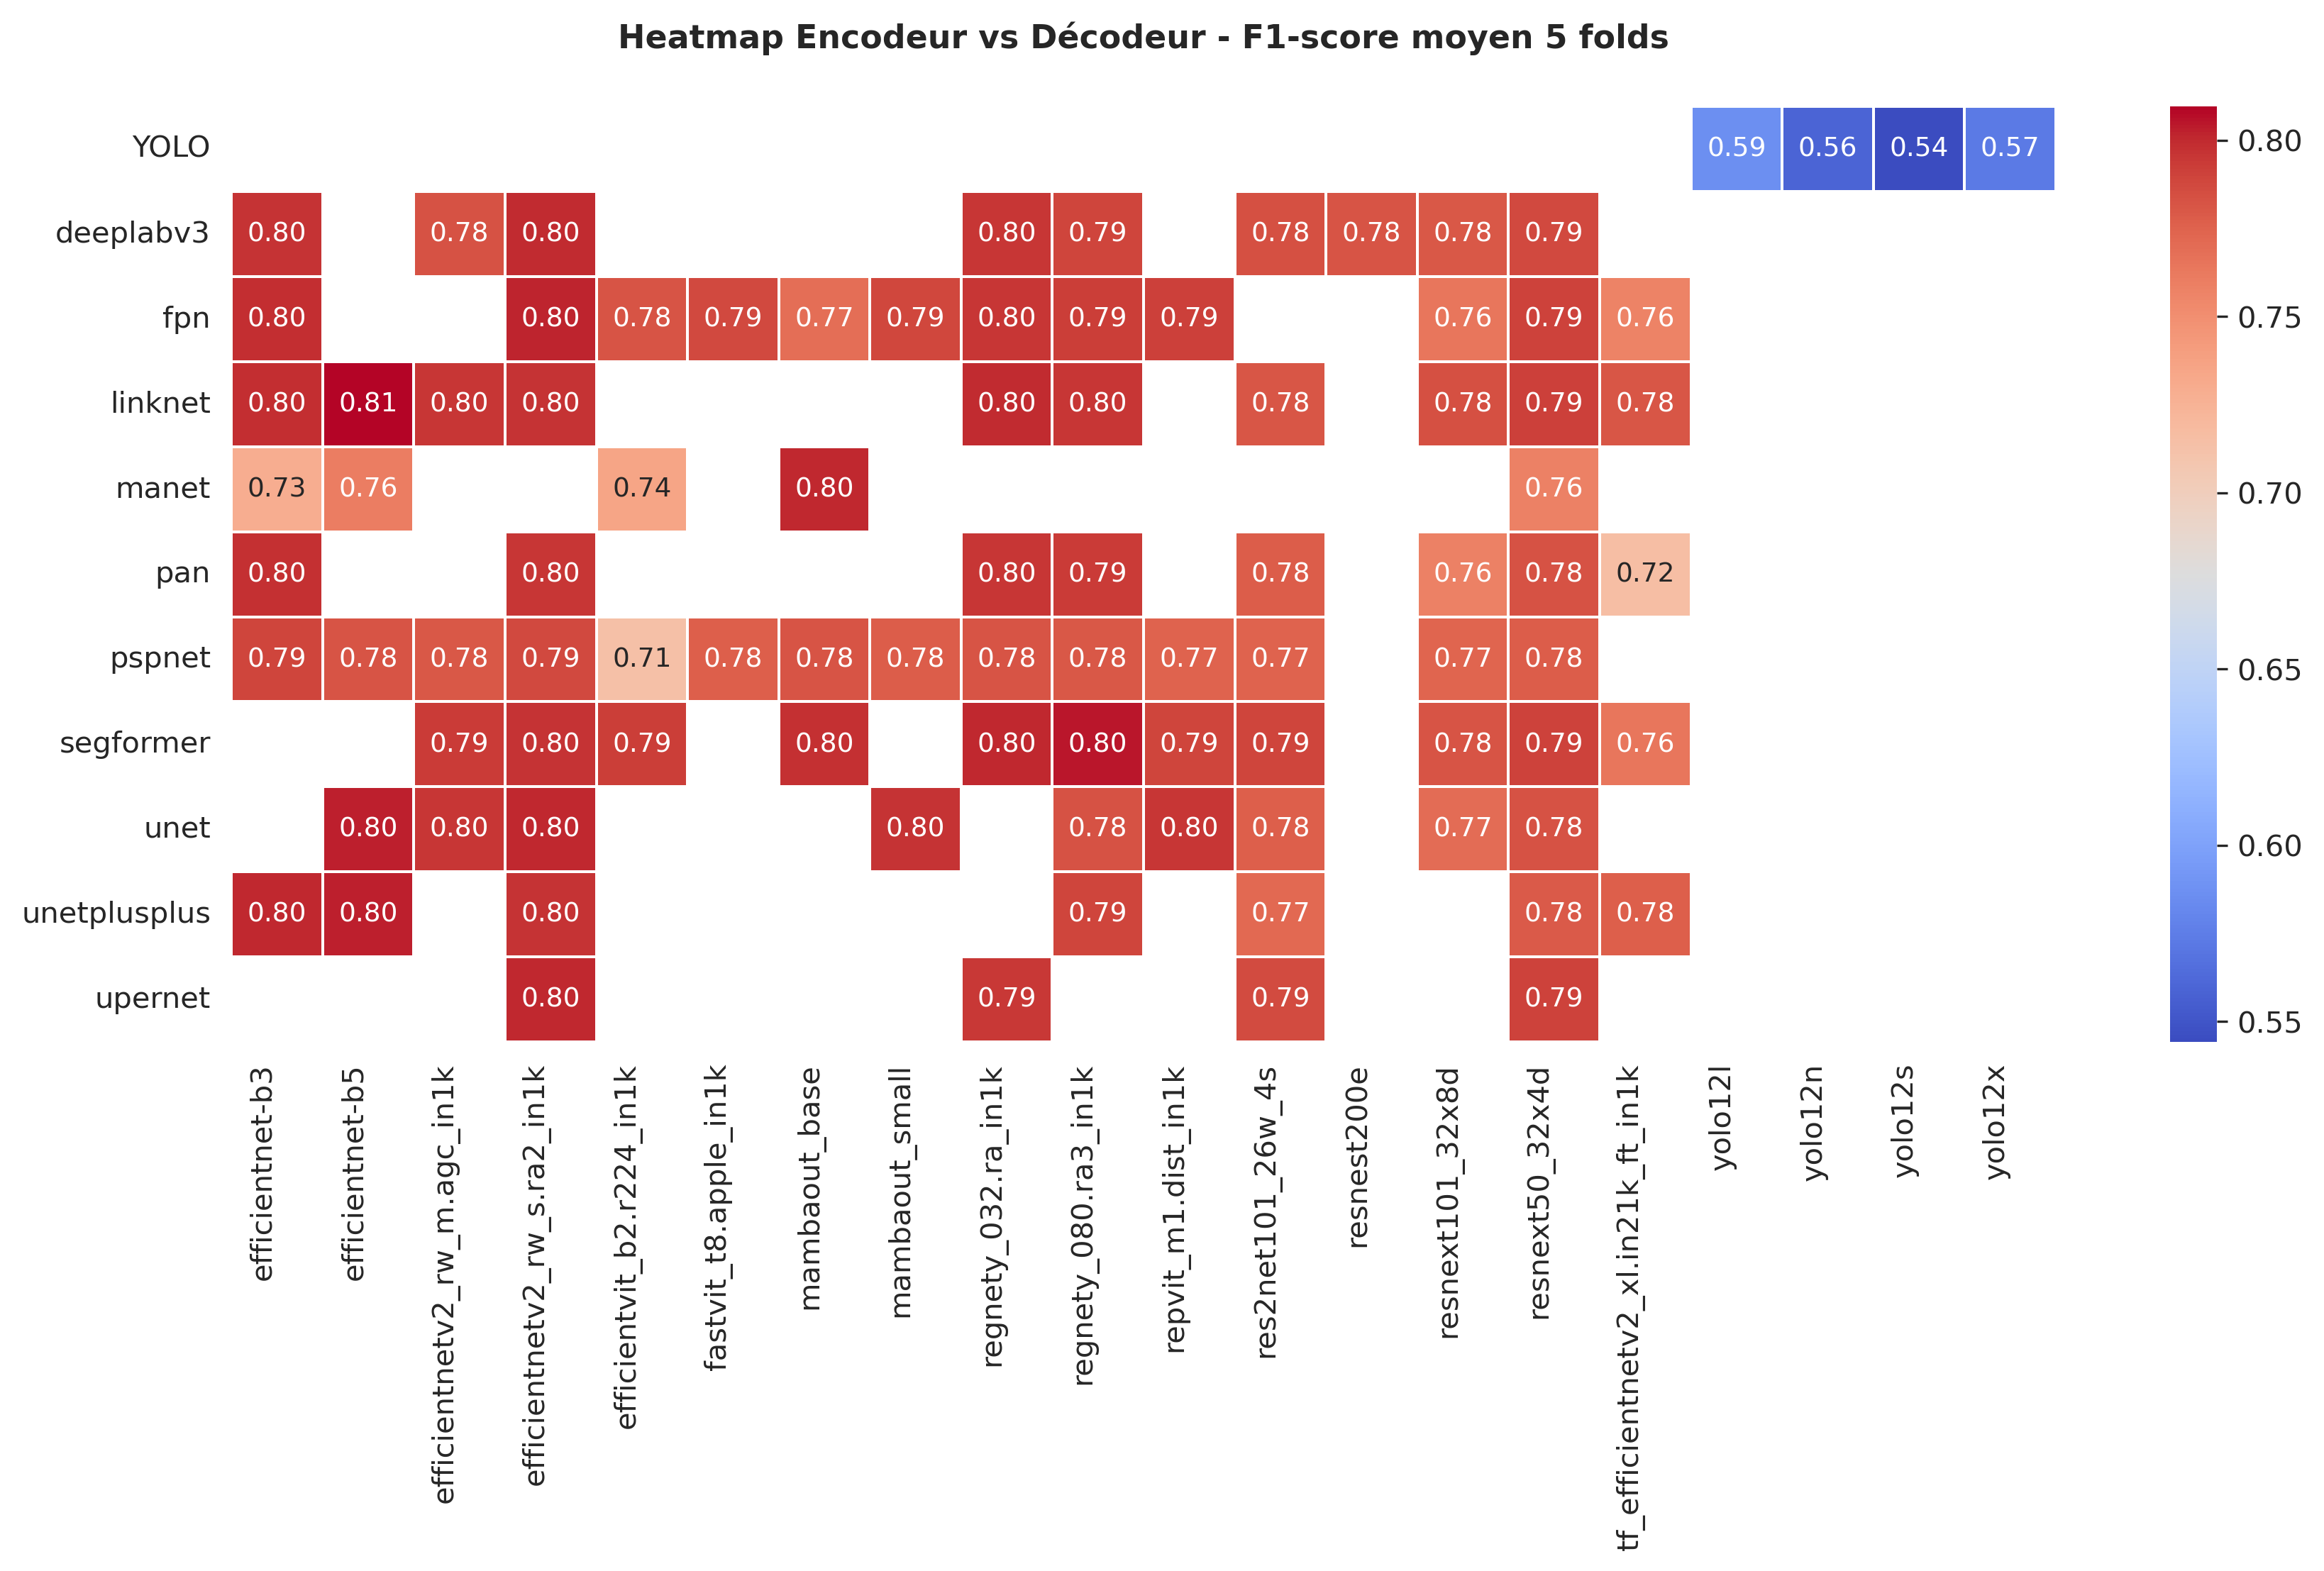
\includegraphics[width=1.45\textwidth]{02-main//figures/ch4/ch4_01_architecture_backbone_heatmap_08_eval_test_f1_score_mean.png}}
    \caption{Heatmap F1-score par combinaison encodeur-décodeur}
    \label{fig:ch4_01_architecture_backbone_heatmap_08_eval_test_f1_score_mean}
\end{figure}

Les modèles YOLOv12 présentent des F1-scores significativement plus faibles que les modèles SMP, malgré des IoU similaires. Cette observation indique que les modèles YOLO peinent à segmenter correctement les espaces libres sur les toitures, ce qui constitue un aspect crucial pour cette tâche. Par exemple, YOLOv12n atteint un IoU de 0,73 mais un F1-score de seulement 0,57, suggérant qu'il génère un nombre important de faux positifs ou de faux négatifs.

\subsubsection{Top 10 des modèles}

La Figure~\ref{fig:ch4_02_top_models_performance_01_eval_test_iou_mean} illustre les 10 meilleurs modèles selon leur IoU.

\begin{figure}[H]
    \centering
    \makebox[\textwidth][c]{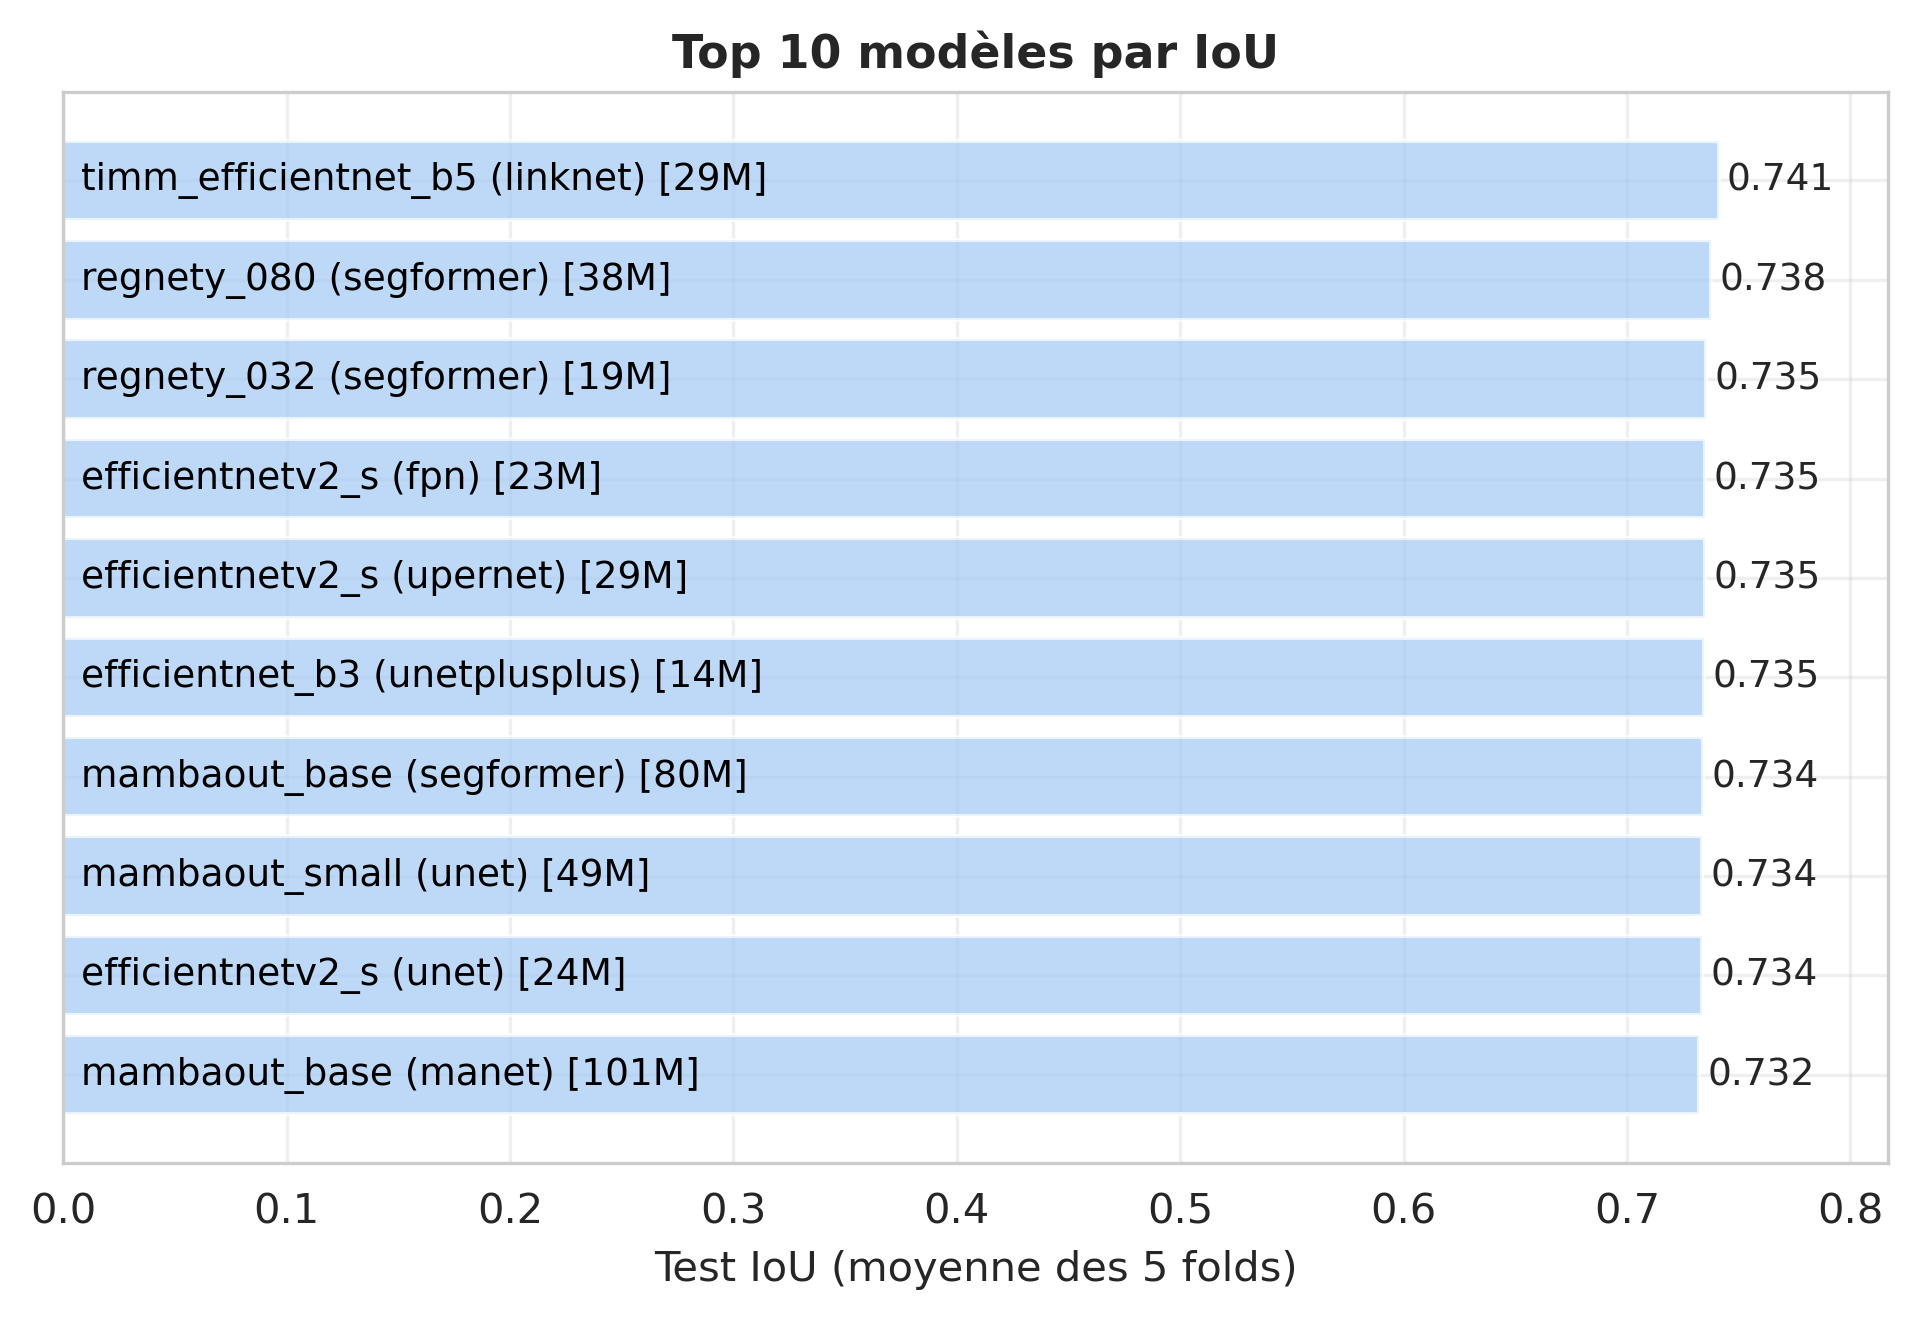
\includegraphics[width=1.10\textwidth]{02-main//figures/ch4/ch4_02_top_models_performance_01_eval_test_iou_mean.png}}
    \caption{Top 10 des modèles par IoU moyen sur dataset de test}
    \label{fig:ch4_02_top_models_performance_01_eval_test_iou_mean}
\end{figure}

Les Figures \ref{fig:ch4_02_top_models_performance_02_eval_test_map_50_mean}, \ref{fig:ch4_02_top_models_performance_03_eval_test_map_75_mean} et \ref{fig:ch4_02_top_models_performance_04_eval_test_map_95_mean} présentent les performances des modèles selon la métrique mAP à différents seuils d'IoU (0.5, 0.75 et 0.95). La Figure \ref{fig:ch4_02_top_models_performance_08_eval_test_f1_score_mean} présente les performances des modèles selon le F1-score.

\begin{figure}[H]
    \centering
    \makebox[\textwidth][c]{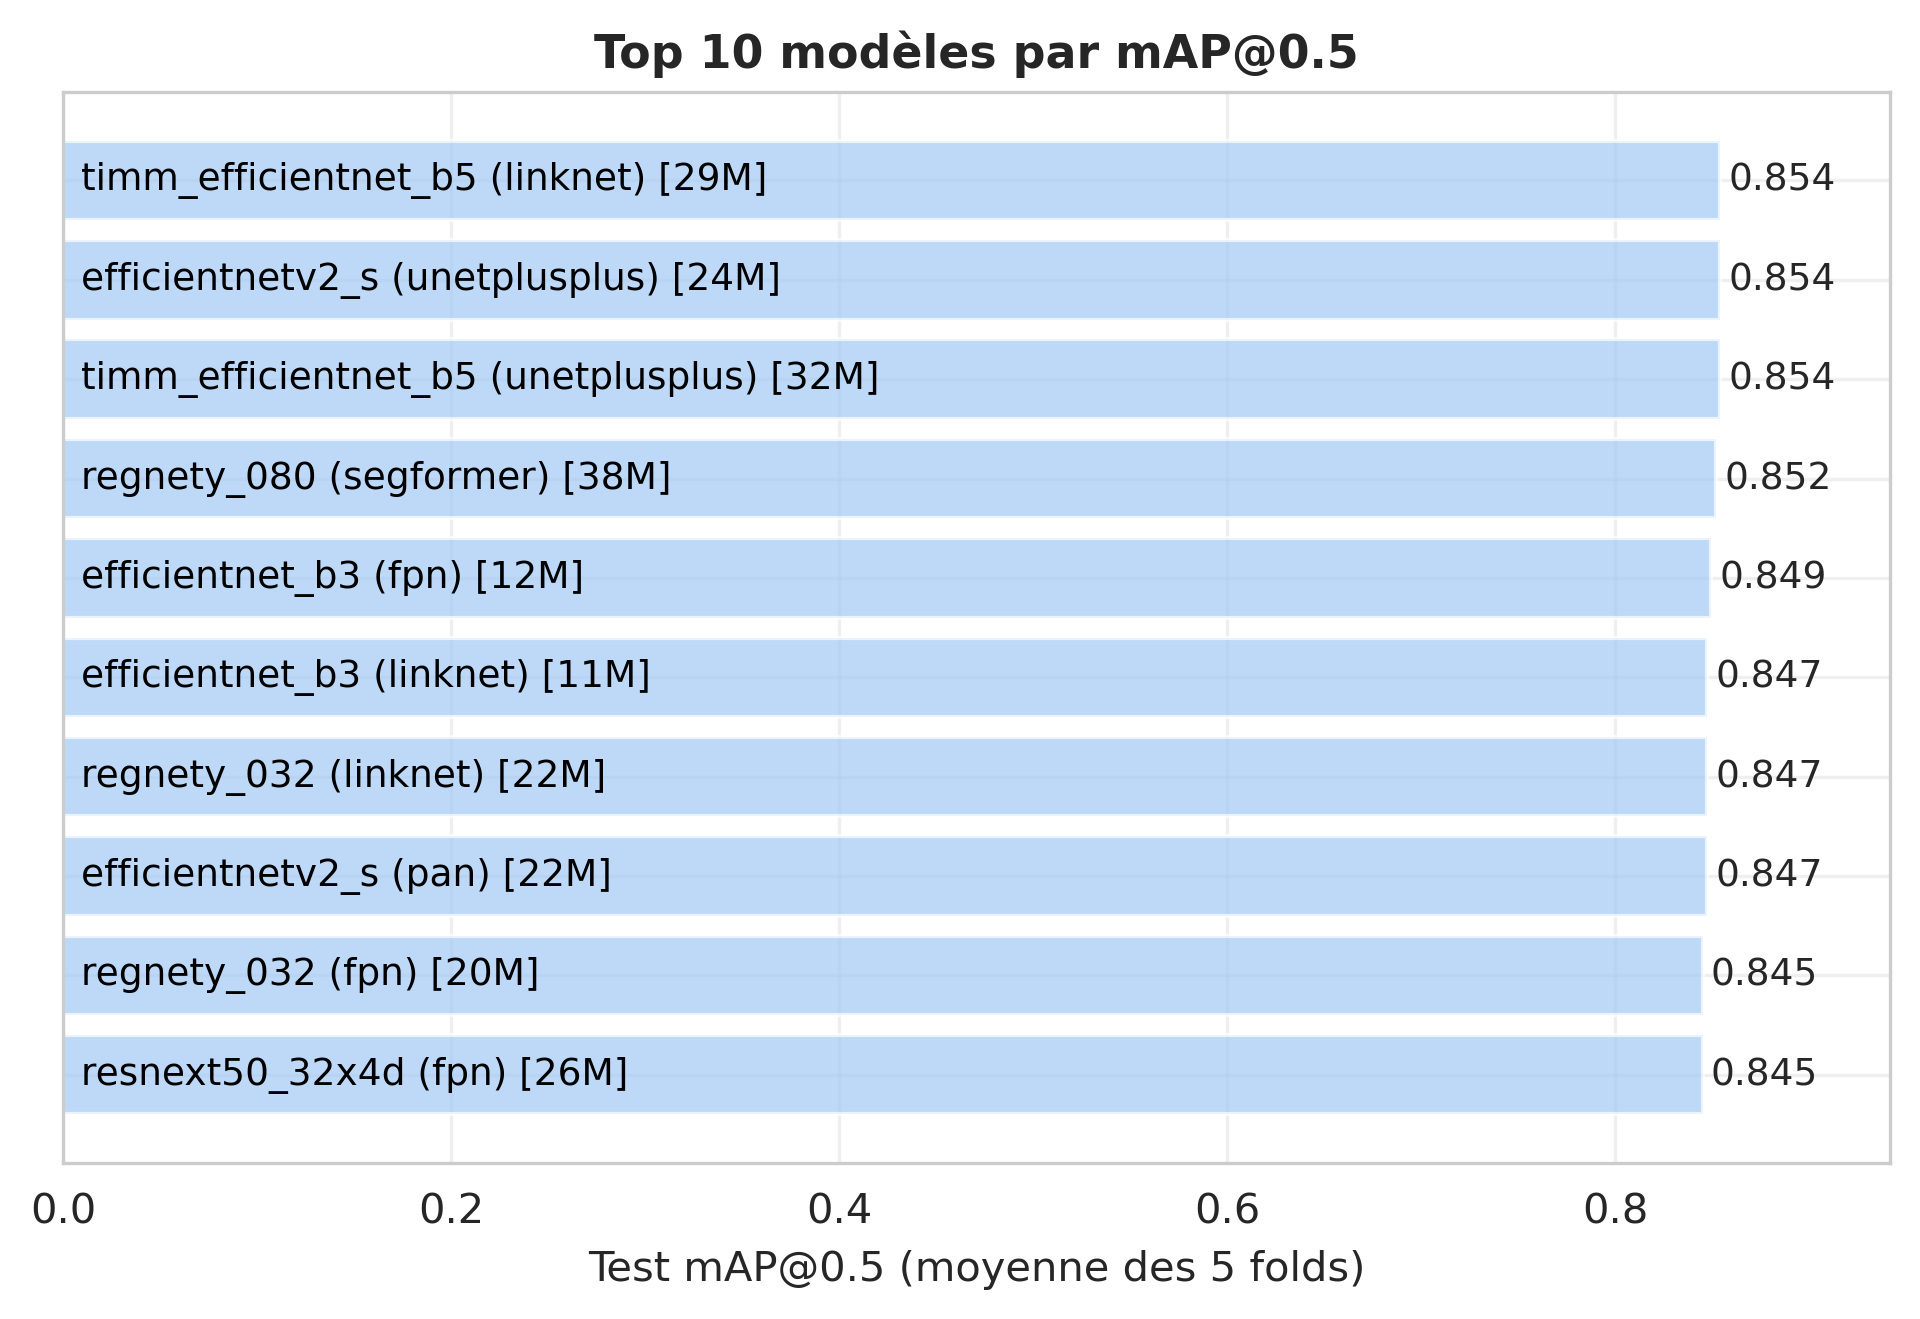
\includegraphics[width=1.05\textwidth]{02-main//figures/ch4/ch4_02_top_models_performance_02_eval_test_map_50_mean.png}}
    \caption{Top 10 des modèles par mAP@0.5 moyen sur dataset de test}
    \label{fig:ch4_02_top_models_performance_02_eval_test_map_50_mean}
\end{figure}

\begin{figure}[H]
    \centering
    \makebox[\textwidth][c]{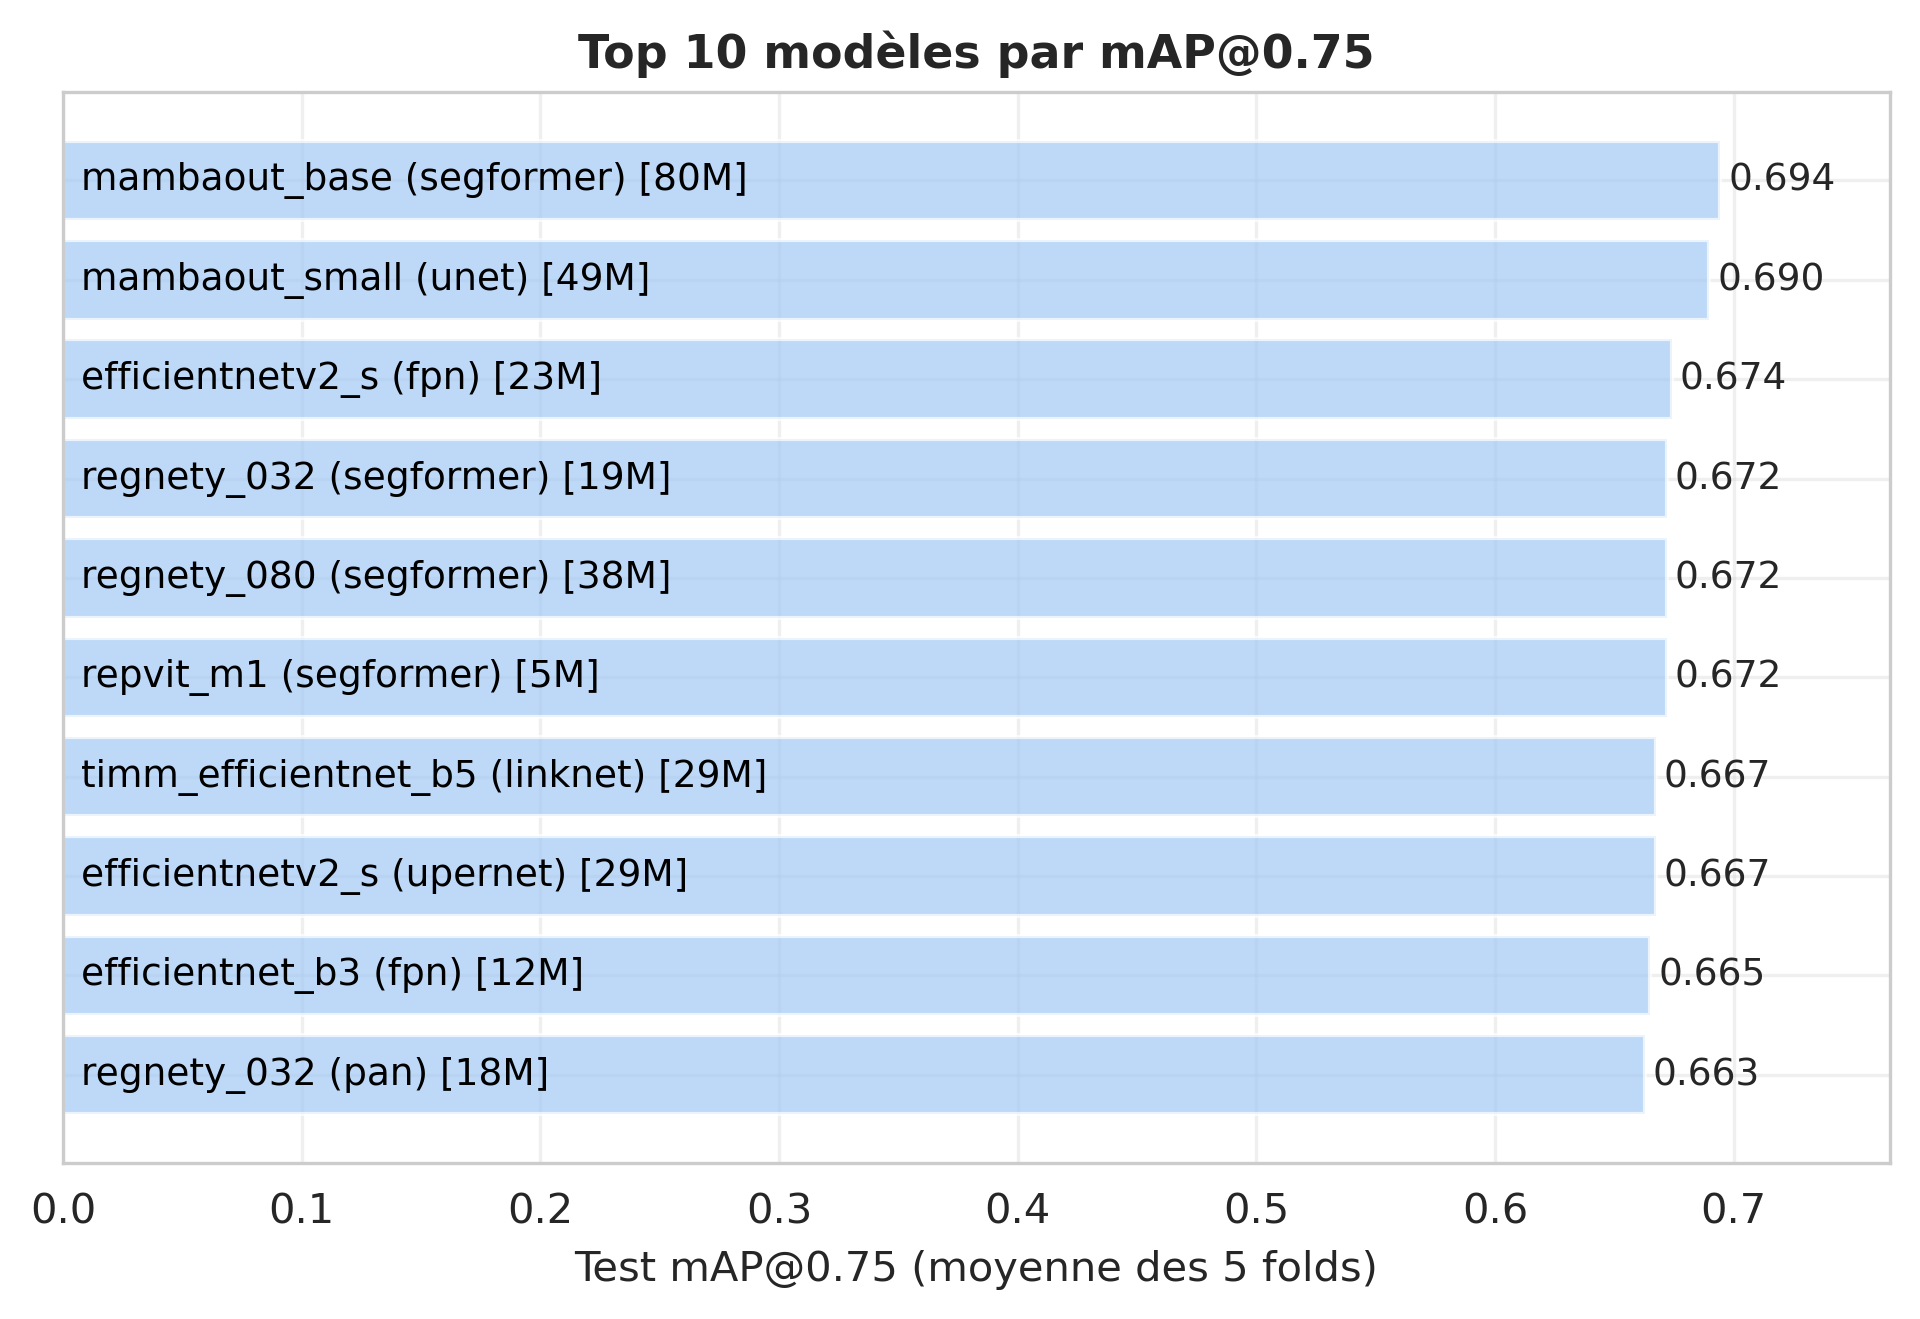
\includegraphics[width=1.05\textwidth]{02-main//figures/ch4/ch4_02_top_models_performance_03_eval_test_map_75_mean.png}}
    \caption{Top 10 des modèles par mAP@0.75 moyen sur dataset de test}
    \label{fig:ch4_02_top_models_performance_03_eval_test_map_75_mean}
\end{figure}

\begin{figure}[H]
    \centering
    \makebox[\textwidth][c]{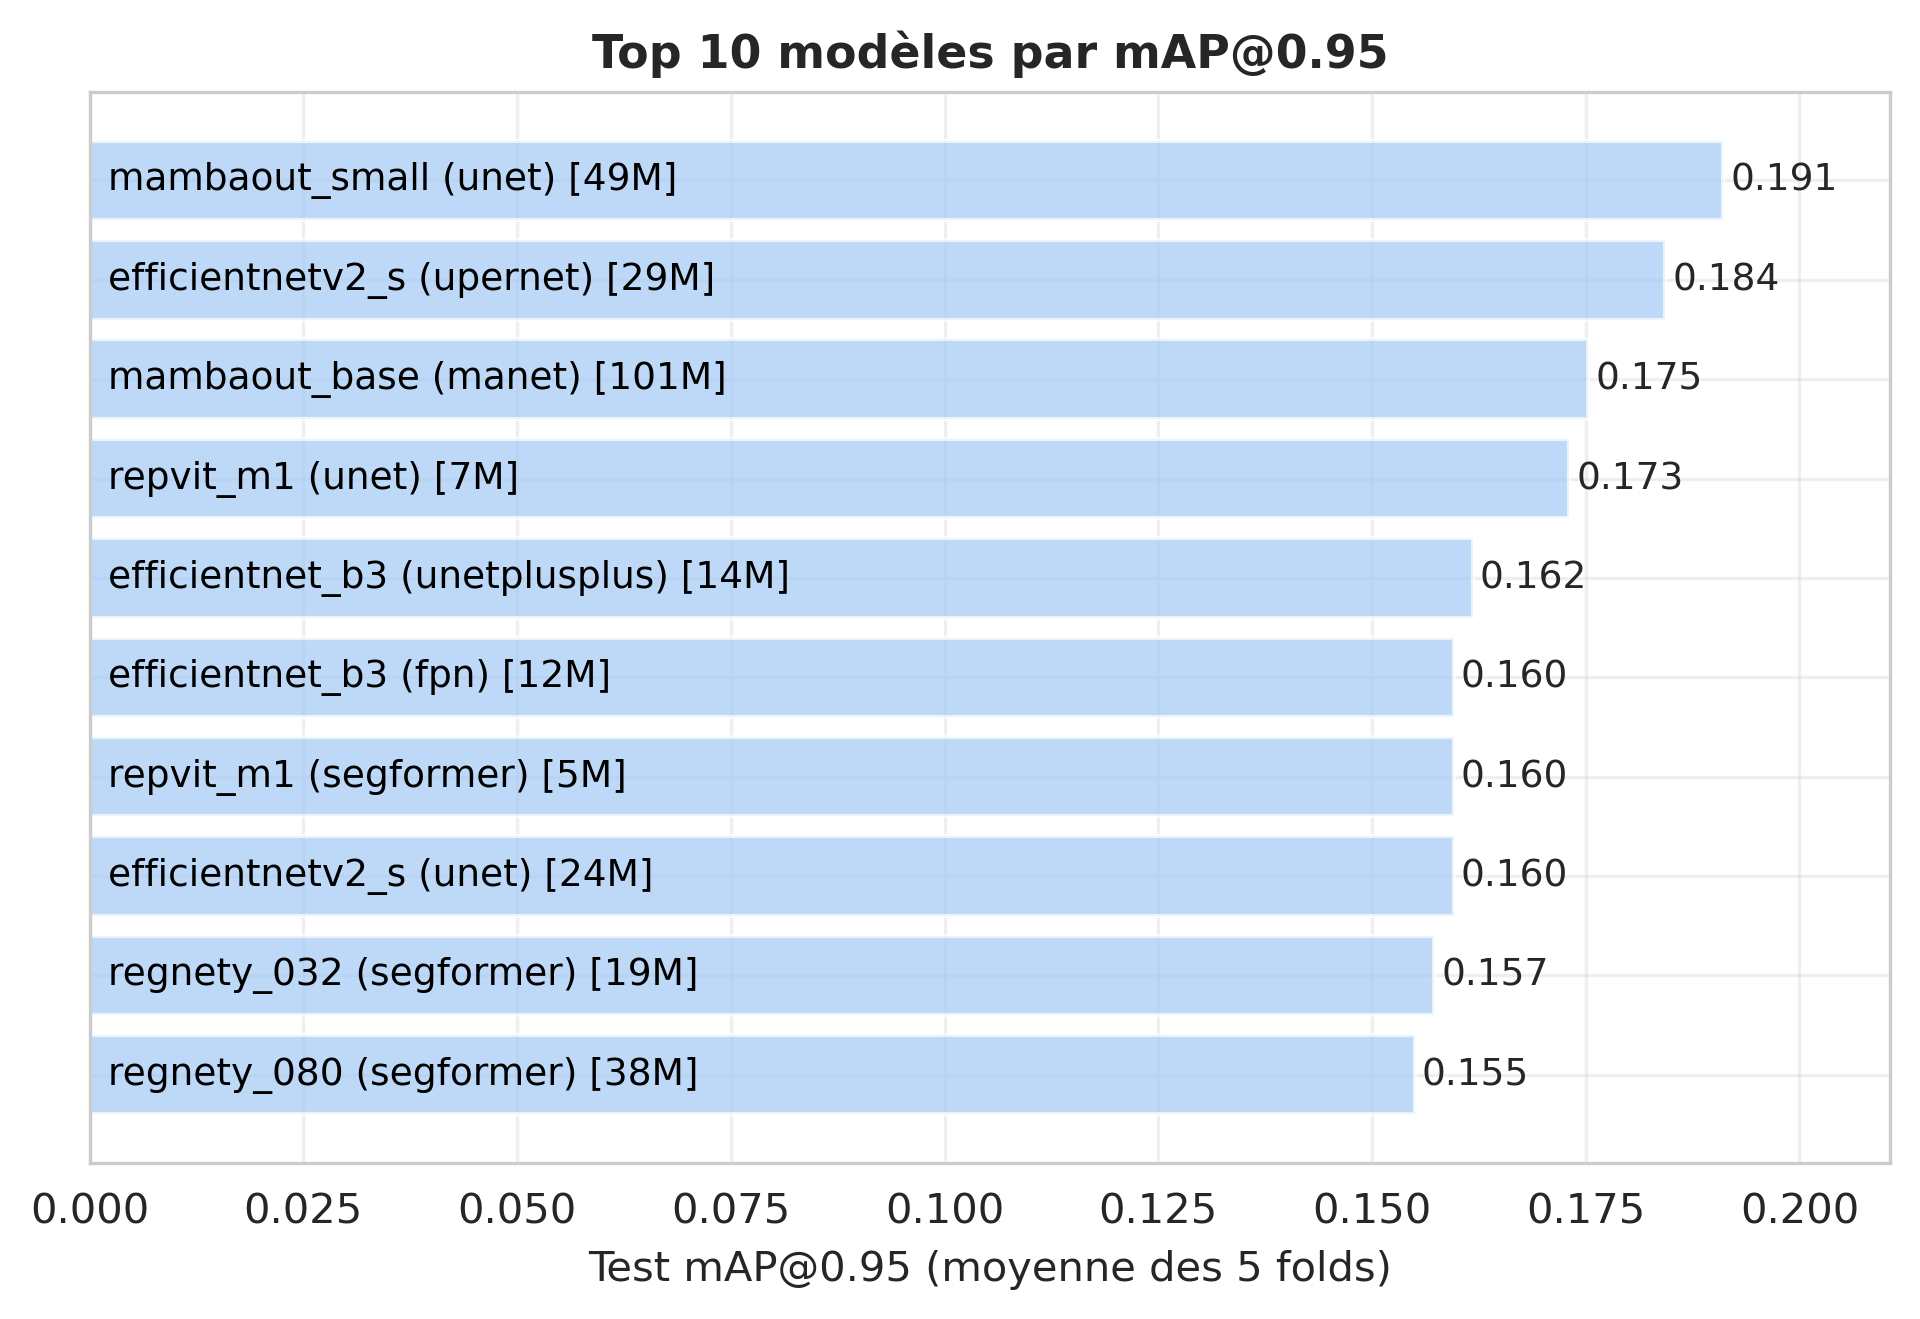
\includegraphics[width=1.05\textwidth]{02-main//figures/ch4/ch4_02_top_models_performance_04_eval_test_map_95_mean.png}}
    \caption{Top 10 des modèles par mAP@0.95 moyen sur dataset de test}
    \label{fig:ch4_02_top_models_performance_04_eval_test_map_95_mean}
\end{figure}

\begin{figure}[H]
    \centering
    \makebox[\textwidth][c]{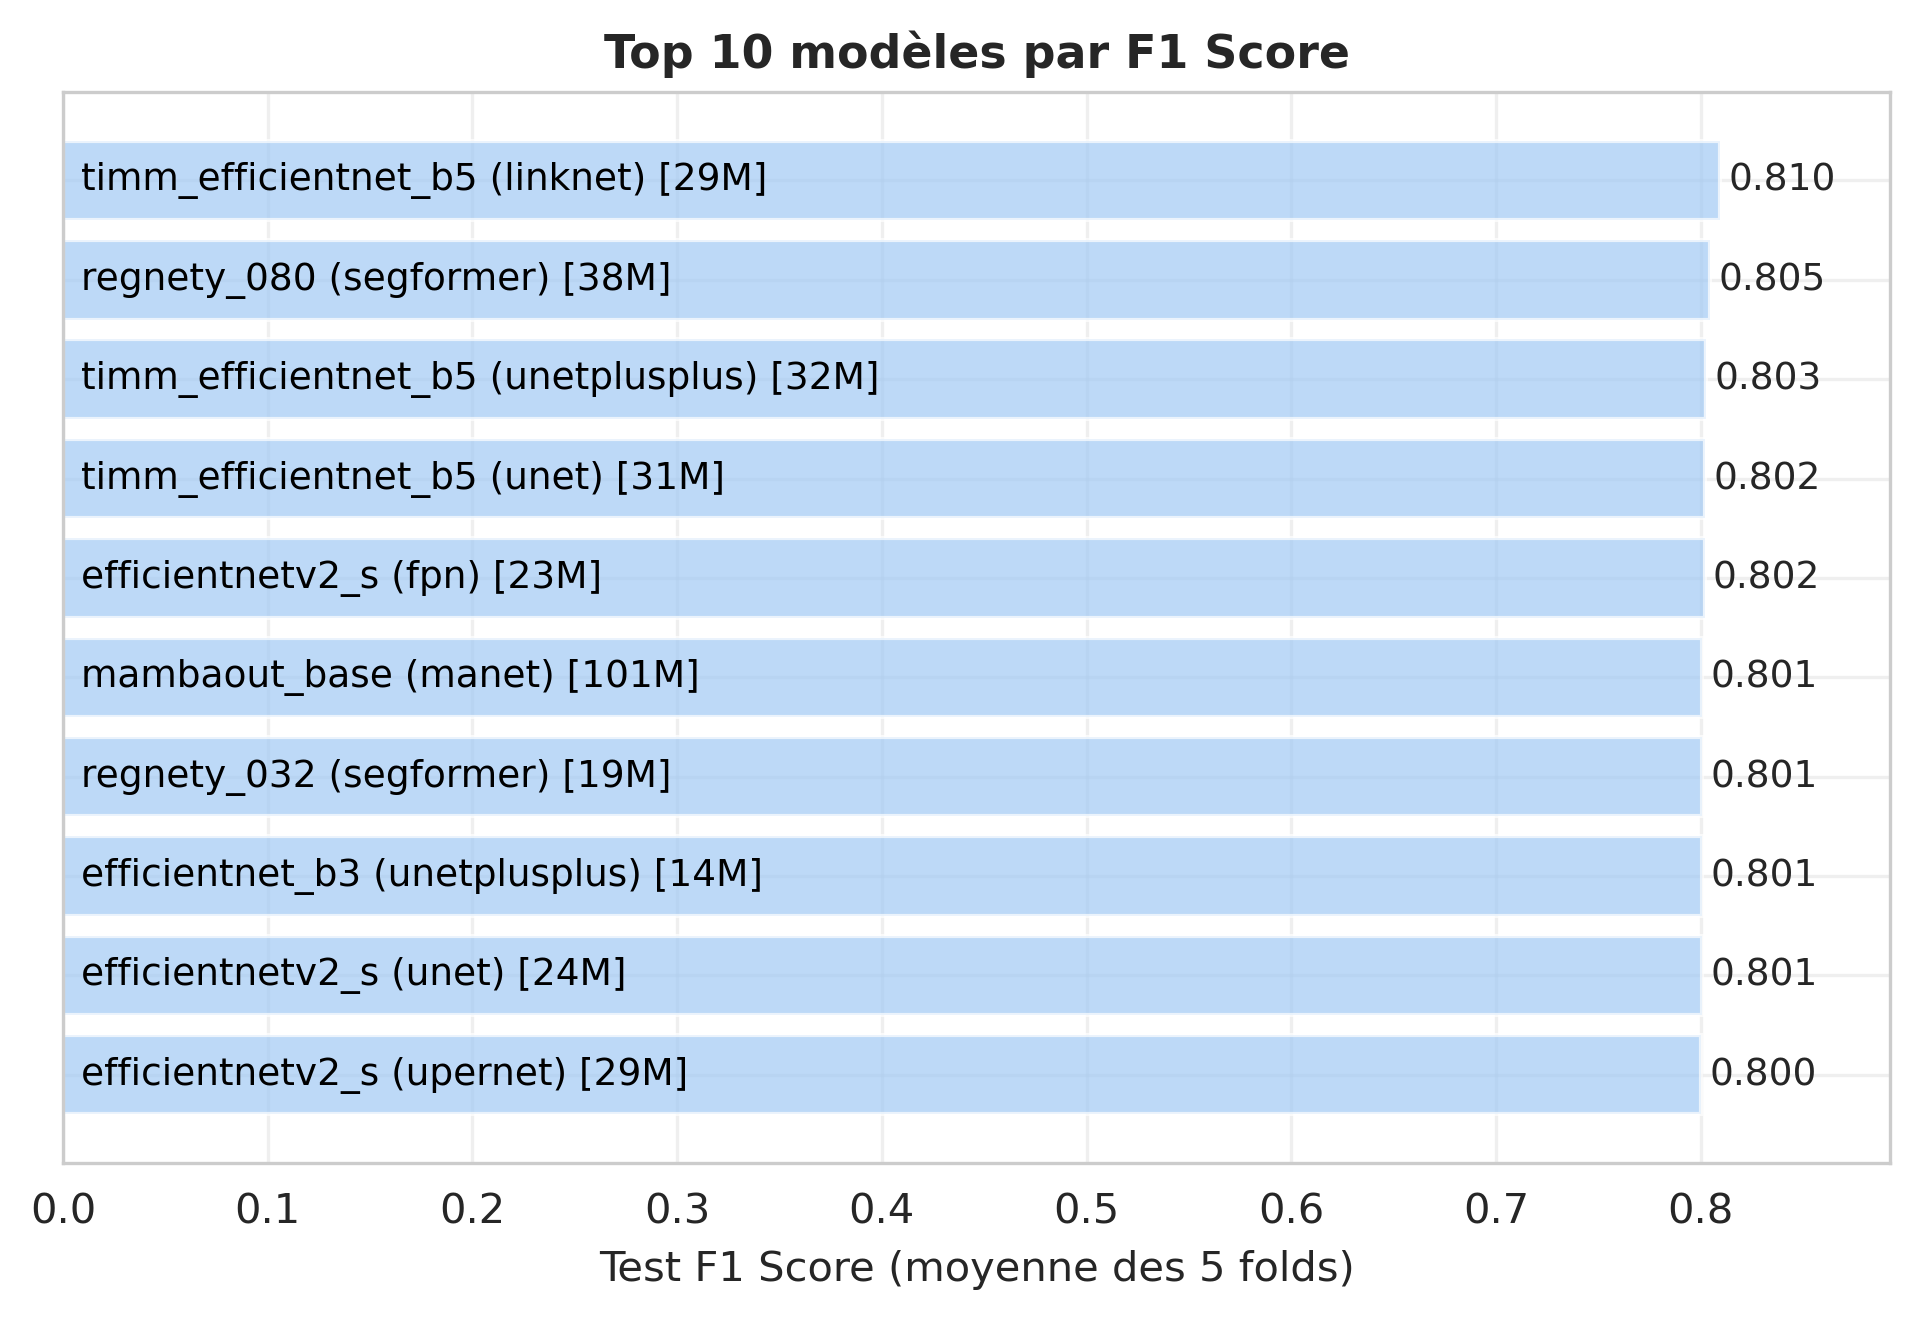
\includegraphics[width=1.05\textwidth]{02-main//figures/ch4/ch4_02_top_models_performance_08_eval_test_f1_score_mean.png}}
    \caption{Top 10 des modèles par F1-score moyen sur dataset de test}
    \label{fig:ch4_02_top_models_performance_08_eval_test_f1_score_mean}
\end{figure}

En résumé, le Tableau~\ref{tab:top10_modeles} présente les 10 meilleurs modèles selon l'IoU moyen sur les 5 fold :

\begin{table}[H]
    \centering
    \makebox[\textwidth][c]{%
    \begin{tabular}{lccccccc}
        \toprule
        Modèle & IoU & F1-Score & mAP@50 & mAP@75 & mAP@95 & Params (M) & Temps (h) \\
        \midrule
        \makecell[l]{Linknet +\\EfficientNet-B5} & 0.741 & 0.810 & 0.854 & 0.667 & 0.151 & 28.75 & 18.11 \\
        \makecell[l]{Segformer +\\RegNetY-080} & 0.738 & 0.805 & 0.852 & 0.672 & 0.155 & 38.41 &  9.29 \\
        \makecell[l]{Segformer +\\RegNetY-032} & 0.735 & 0.801 & 0.831 & 0.672 & 0.157 & 18.87 & 30.62 \\
        \makecell[l]{FPN +\\EfficientNetV2-S} & 0.735 & 0.802 & 0.834 & 0.674 & 0.153 & 23.42 & 19.56 \\
        \makecell[l]{Upernet +\\EfficientNetV2-S} & 0.735 & 0.800 & 0.840 & 0.667 & 0.184 & 29.13 & 27.75 \\
        \makecell[l]{Unetplusplus +\\EfficientNet-B5} & 0.735 & 0.801 & 0.843 & 0.661 & 0.162 & 13.63 & 31.28 \\
        \makecell[l]{Segformer +\\mambaout\_base} & 0.734 & 0.797 & 0.820 & 0.694 & 0.153 & 80.06 &  5.93 \\
        \makecell[l]{Unet +\\mambaout\_small} & 0.734 & 0.796 & 0.827 & 0.690 & 0.191 & 48.52 &  8.95 \\
        \makecell[l]{Unet +\\EfficientNetV2-S} & 0.734 & 0.801 & 0.845 & 0.647 & 0.160 & 23.94 & 23.45 \\
        \makecell[l]{Manet +\\mambaout\_small} & 0.732 & 0.801 & 0.845 & 0.656 & 0.175 & 100.61 &  9.94 \\
        \bottomrule
    \end{tabular}%
    }
    \caption{Top 10 des modèles par IoU moyen sur dataset de test}
    \label{tab:top10_modeles}
\end{table}

Le mAP (mean Average Precision) constitue une métrique qui évalue la capacité d'un modèle à détecter et délimiter avec précision les espaces libres sur les toitures. Le mAP permet de vérifier non seulement si le modèle identifie les bonnes zones, mais aussi à quel point il les délimite précisément.

L'IoU représente le rapport entre la surface de chevauchement et la surface totale couverte par la prédiction du modèle et la vérité terrain. Un IoU de 0,5 signifie que la zone détectée chevauche d'au moins 50\% avec la zone réelle. Plus le seuil IoU est élevé, plus la détection doit être précise pour être considérée comme correcte.

Le mAP se décline en plusieurs variantes selon le niveau de précision requis :

\begin{itemize}
    \item mAP@50
    \begin{itemize}
        \item Accepte les détections avec 50\% de chevauchement minimum
        \item Suffisant pour identifier l'emplacement général des espaces libres
    \end{itemize}
    \item mAP@75
    \begin{itemize}
        \item Exige 75\% de chevauchement minimum
        \item Assure que les contours détectés sont relativement fidèles à la réalité
    \end{itemize}
    \item mAP@95
    \begin{itemize}
        \item Requiert 95\% de chevauchement minimum
        \item Segmentation très précise et fiable
    \end{itemize}
\end{itemize}

Un modèle performant devra atteindre des scores élevés sur ces trois seuils pour être considéré comme adapté à une utilisation opérationnelle.

L'analyse du mAP@95 (Figure \ref{fig:ch4_02_top_models_performance_04_eval_test_map_95_mean}) révèle qu'UNet avec mambaout\_small obtient les meilleures performances avec un score de 0,191. Ce modèle affiche également un mAP@75 de 0,690 et un mAP@50 de 0,827. UNet++ avec EfficientNet-B5 se distingue également avec un mAP@95 de 0,162, accompagné d'un mAP@75 de 0,661 et d'un mAP@50 de 0,843.

Ces performances indiquent que ces modèles sont capables de segmenter précisément les espaces libres sur les toitures, même dans des conditions architecturales complexes, ce qui confirme leur potentiel pour une application opérationnelle.

\subsection{Analyse comparative des architectures}

\subsubsection{Performance par famille de décodeur}

L'analyse des performances par décodeur selon les métriques IoU (Figure \ref{fig:ch4_06_architecture_boxplot_01_eval_test_iou_mean} et Tableau \ref{tab:statistique_par_decodeur_iou}) et mAP@0.95 (Figure \ref{fig:ch4_06_architecture_boxplot_04_eval_test_map_95_mean} et Tableau \ref{tab:statistique_par_decodeur_map95}) révèle des tendances significatives.

\begin{figure}[H]
    \centering
    \makebox[\textwidth][c]{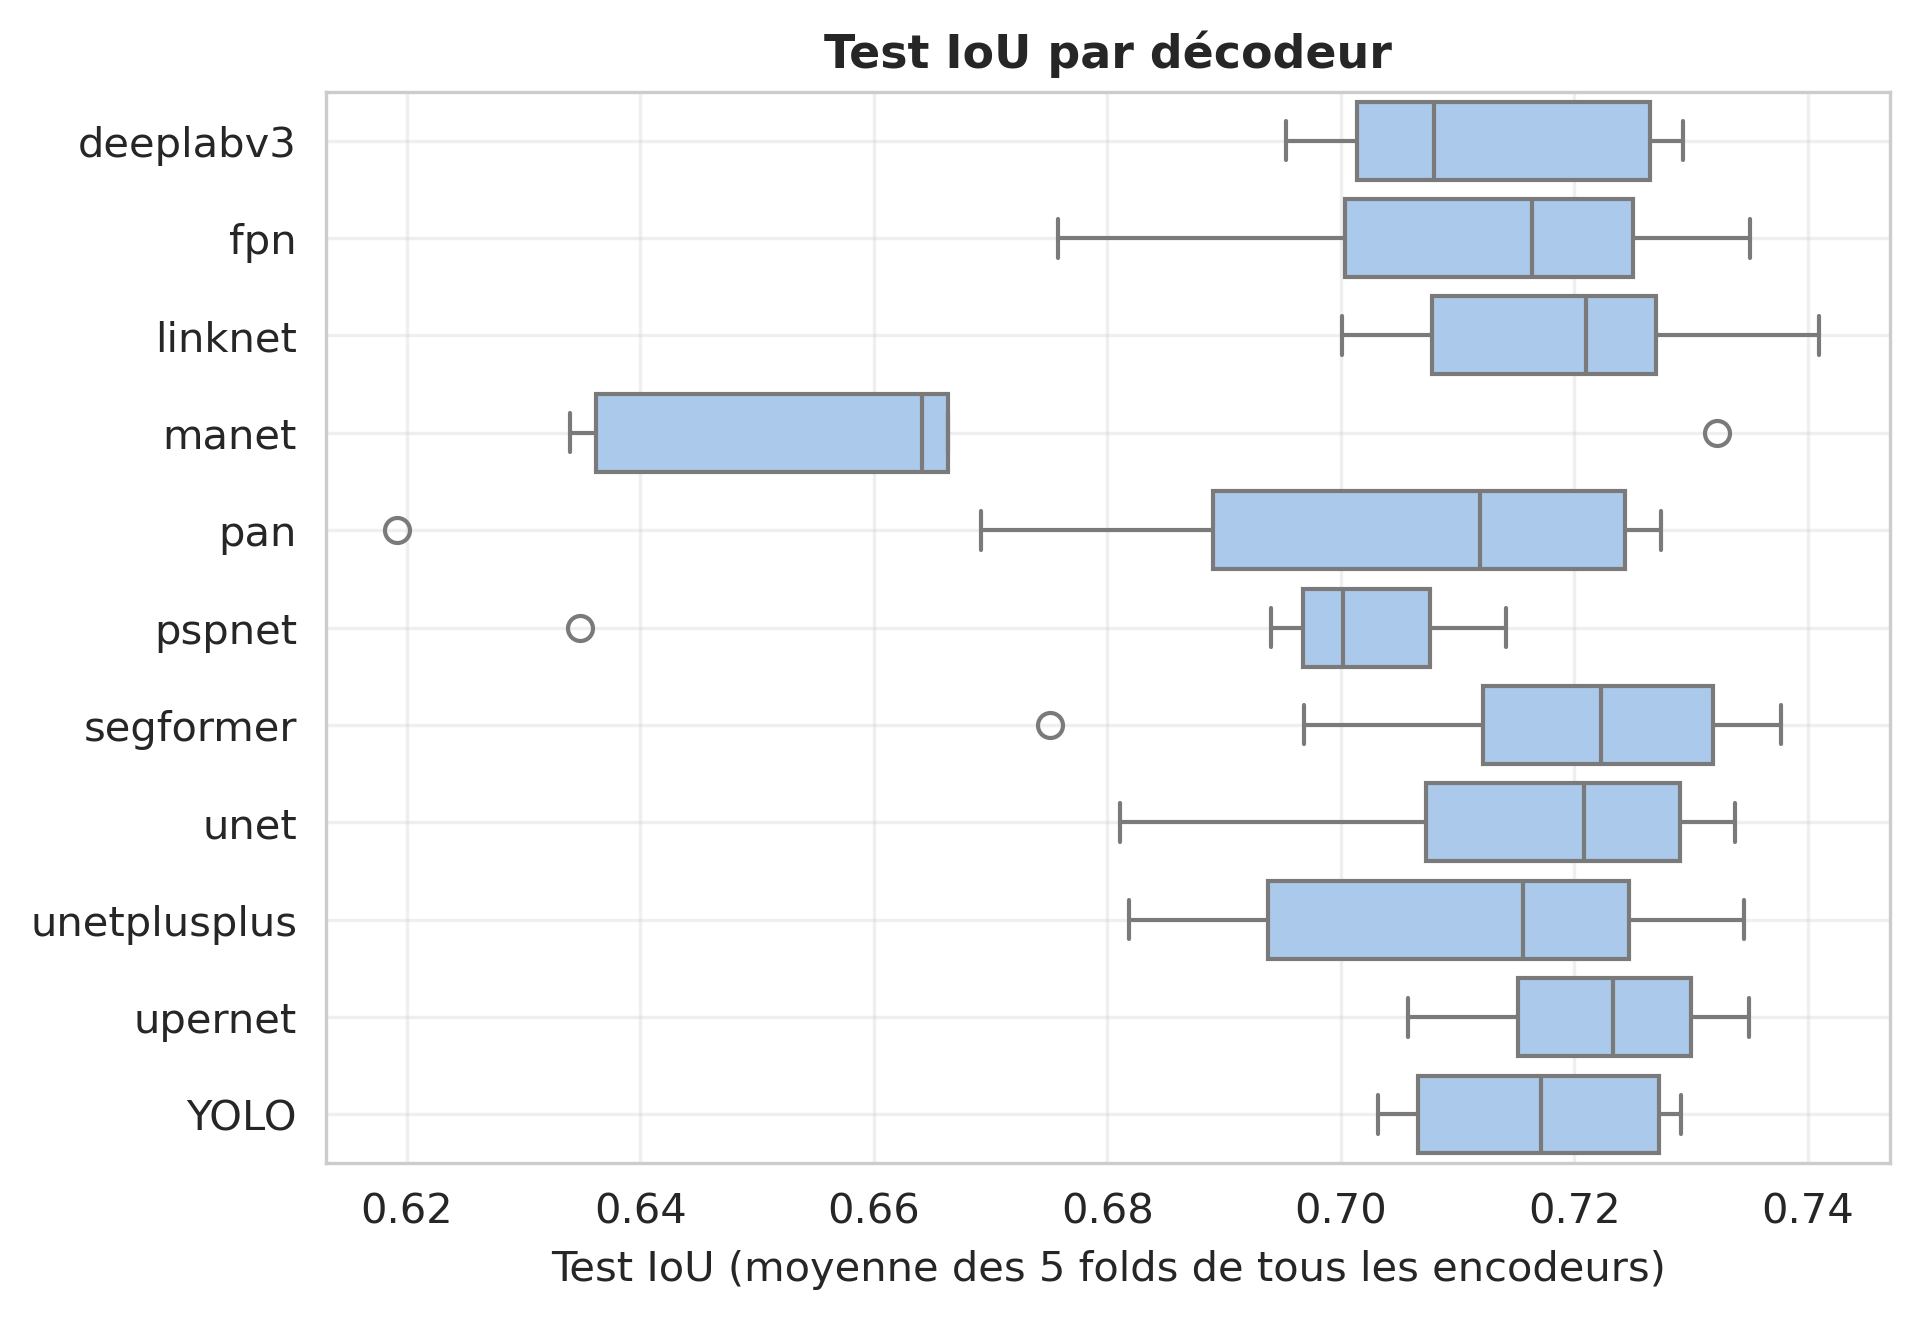
\includegraphics[width=1.05\textwidth]{02-main//figures/ch4/ch4_06_architecture_boxplot_01_eval_test_iou_mean.png}}
    \caption{Boîte à moustaches IoU par décodeur}
    \label{fig:ch4_06_architecture_boxplot_01_eval_test_iou_mean}
\end{figure}

\begin{table}[H]
    \centering
    \begin{tabular}{lccccc}
    \toprule
    Décodeur & \multicolumn{5}{c}{IoU} \\
    & Moyenne & écart-type & Médiane & Minimum & Maximum \\
    \midrule
    YOLO & 0.717 & 0.013 & 0.717 & 0.703 & 0.729 \\
    deeplabv3 & 0.712 & 0.014 & 0.708 & 0.695 & 0.729 \\
    fpn & 0.711 & 0.020 & 0.716 & 0.676 & 0.735 \\
    linknet & 0.719 & 0.013 & 0.721 & 0.700 & 0.741 \\
    manet & 0.667 & 0.040 & 0.664 & 0.634 & 0.732 \\
    pan & 0.698 & 0.038 & 0.712 & 0.619 & 0.727 \\
    pspnet & 0.697 & 0.019 & 0.700 & 0.635 & 0.714 \\
    segformer & 0.718 & 0.019 & 0.722 & 0.675 & 0.738 \\
    unet & 0.715 & 0.018 & 0.721 & 0.681 & 0.734 \\
    unetplusplus & 0.710 & 0.020 & 0.716 & 0.682 & 0.735 \\
    upernet & 0.722 & 0.013 & 0.723 & 0.706 & 0.735 \\
    \bottomrule
    \end{tabular}
    \caption{Statistiques IoU par décodeur}
    \label{tab:statistique_par_decodeur_iou}
\end{table}

\begin{figure}[H]
    \centering
    \makebox[\textwidth][c]{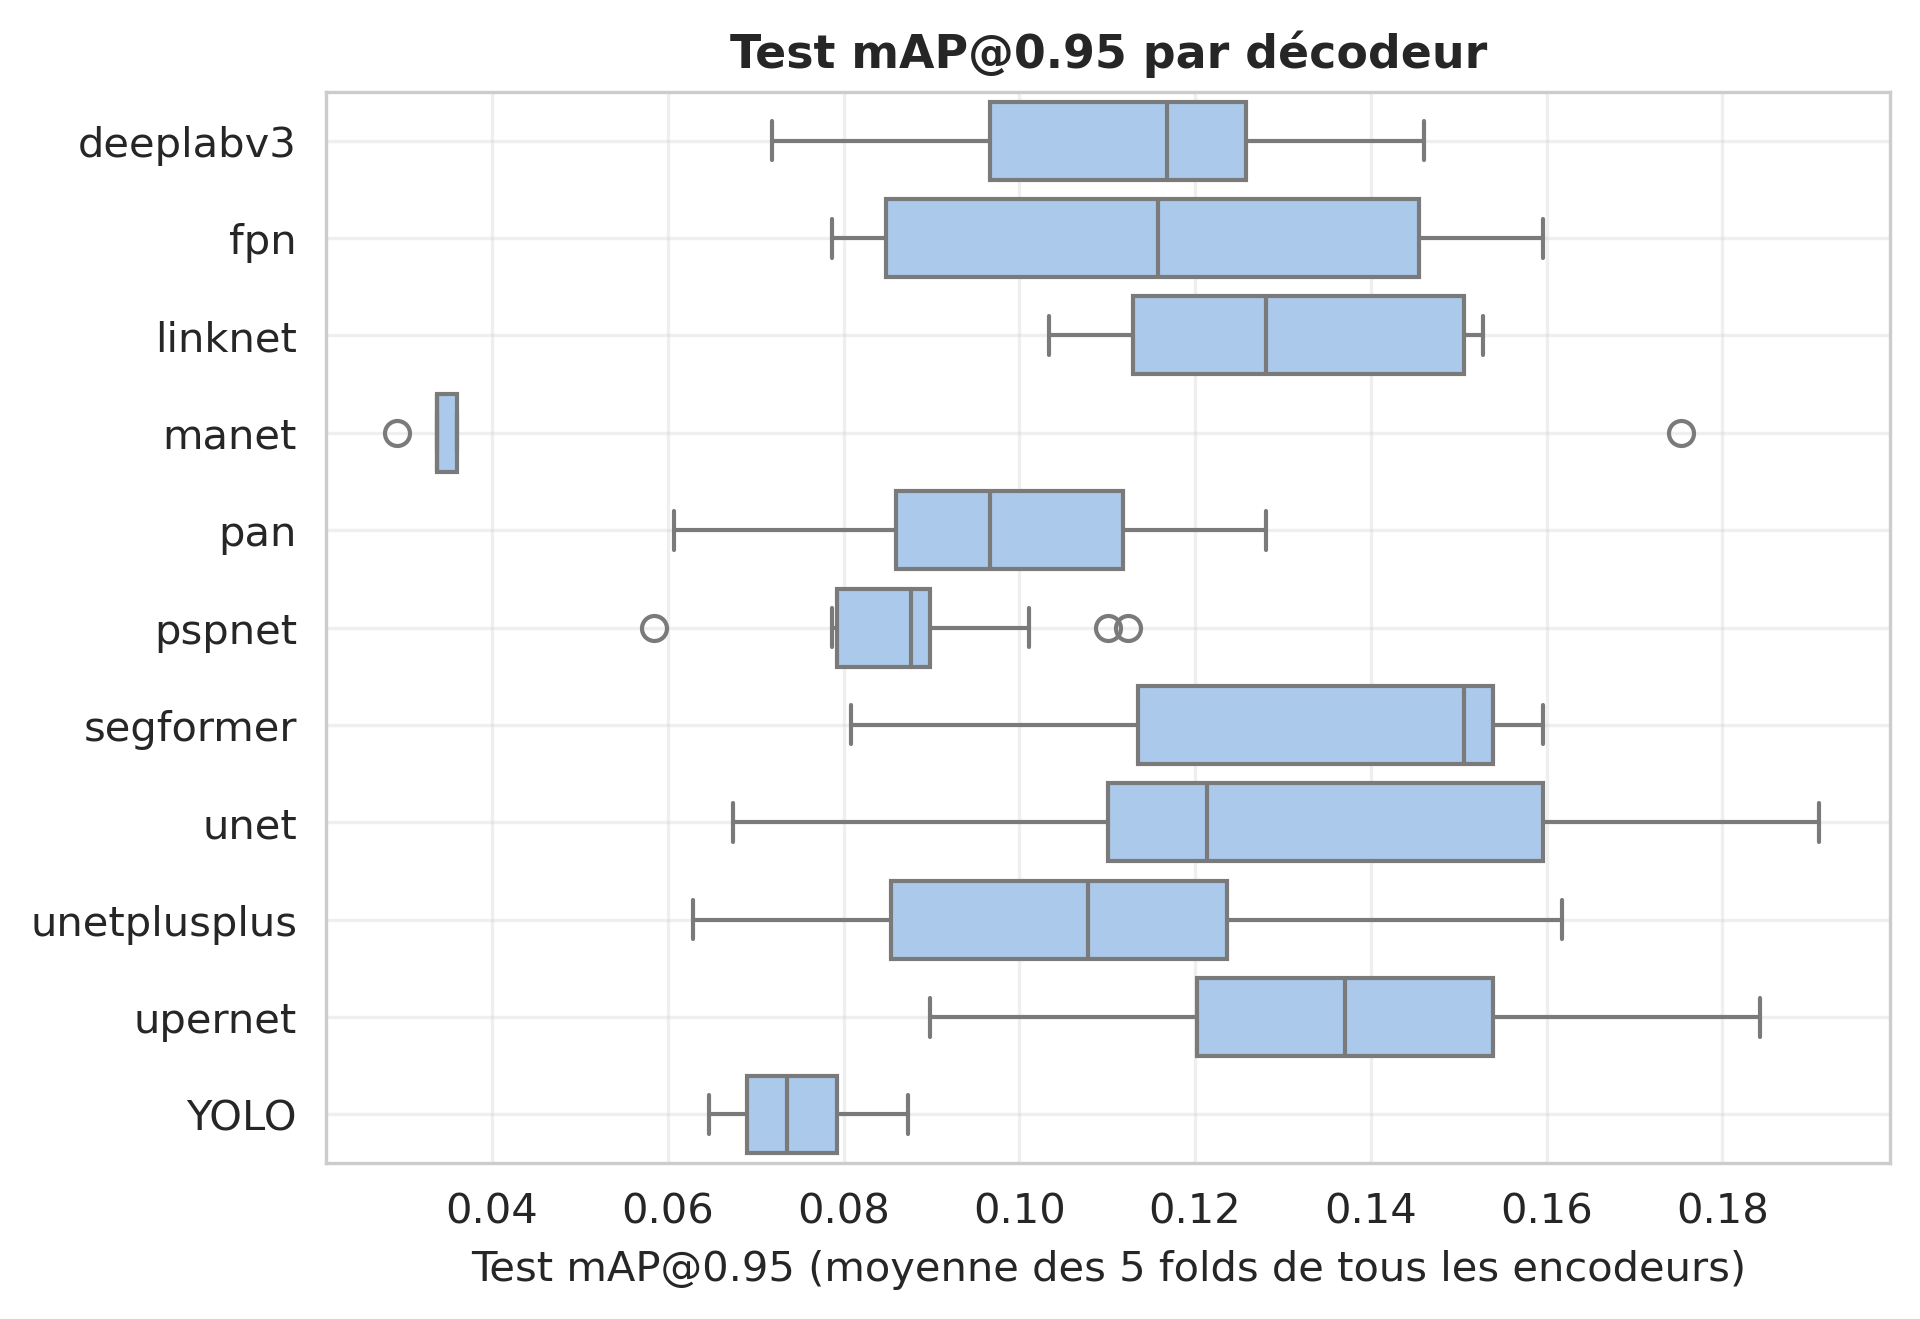
\includegraphics[width=1.05\textwidth]{02-main//figures/ch4/ch4_06_architecture_boxplot_04_eval_test_map_95_mean.png}}
    \caption{Boîte à moustaches mAP@95 par décodeur}
    \label{fig:ch4_06_architecture_boxplot_04_eval_test_map_95_mean}
\end{figure}

\begin{table}[H]
    \centering
    \begin{tabular}{lccccc}
    \toprule
    Décodeur & \multicolumn{5}{c}{mAP@0.95} \\
    & Moyenne & écart-type & Médiane & Minimum & Maximum \\
    \midrule
    YOLO & 0.075 & 0.010 & 0.074 & 0.065 & 0.087 \\
    deeplabv3 & 0.110 & 0.025 & 0.117 & 0.072 & 0.146 \\
    fpn & 0.116 & 0.032 & 0.116 & 0.079 & 0.160 \\
    linknet & 0.130 & 0.021 & 0.128 & 0.103 & 0.153 \\
    manet & 0.062 & 0.064 & 0.034 & 0.029 & 0.175 \\
    pan & 0.096 & 0.023 & 0.097 & 0.061 & 0.128 \\
    pspnet & 0.087 & 0.014 & 0.088 & 0.058 & 0.112 \\
    segformer & 0.131 & 0.028 & 0.151 & 0.081 & 0.160 \\
    unet & 0.128 & 0.041 & 0.121 & 0.067 & 0.191 \\
    unetplusplus & 0.107 & 0.033 & 0.108 & 0.063 & 0.162 \\
    upernet & 0.137 & 0.039 & 0.137 & 0.090 & 0.184 \\
    \bottomrule
    \end{tabular}
    \caption{Statistiques mAP@0.95 par décodeur}
    \label{tab:statistique_par_decodeur_map95}
\end{table}

Les décodeurs présentent des performances très variables selon les encodeurs choisis, ce qui se manifeste par la variance (largeur des boîtes) et les valeurs extrêmes (moustaches) observées dans les boîtes à moustaches. Certains décodeurs affichent néanmoins des performances globalement inférieures aux autres en termes de mAP@0.95, notamment MANet et YOLOv12.

\subsubsection{Performance par encodeur}

L'analyse des encodeurs avec les métriques IoU (Figure \ref{fig:ch4_07_backbone_boxplot_01_eval_test_iou_mean} et Tableau \ref{tab:statistique_par_encodeur_iou}) et mAP@0.95 (Figure \ref{fig:ch4_07_backbone_boxplot_04_eval_test_map_95_mean} et Tableau \ref{tab:statistique_par_encodeur_map95}) révèle des différences notables.

\begin{figure}[H]
    \centering
    \makebox[\textwidth][c]{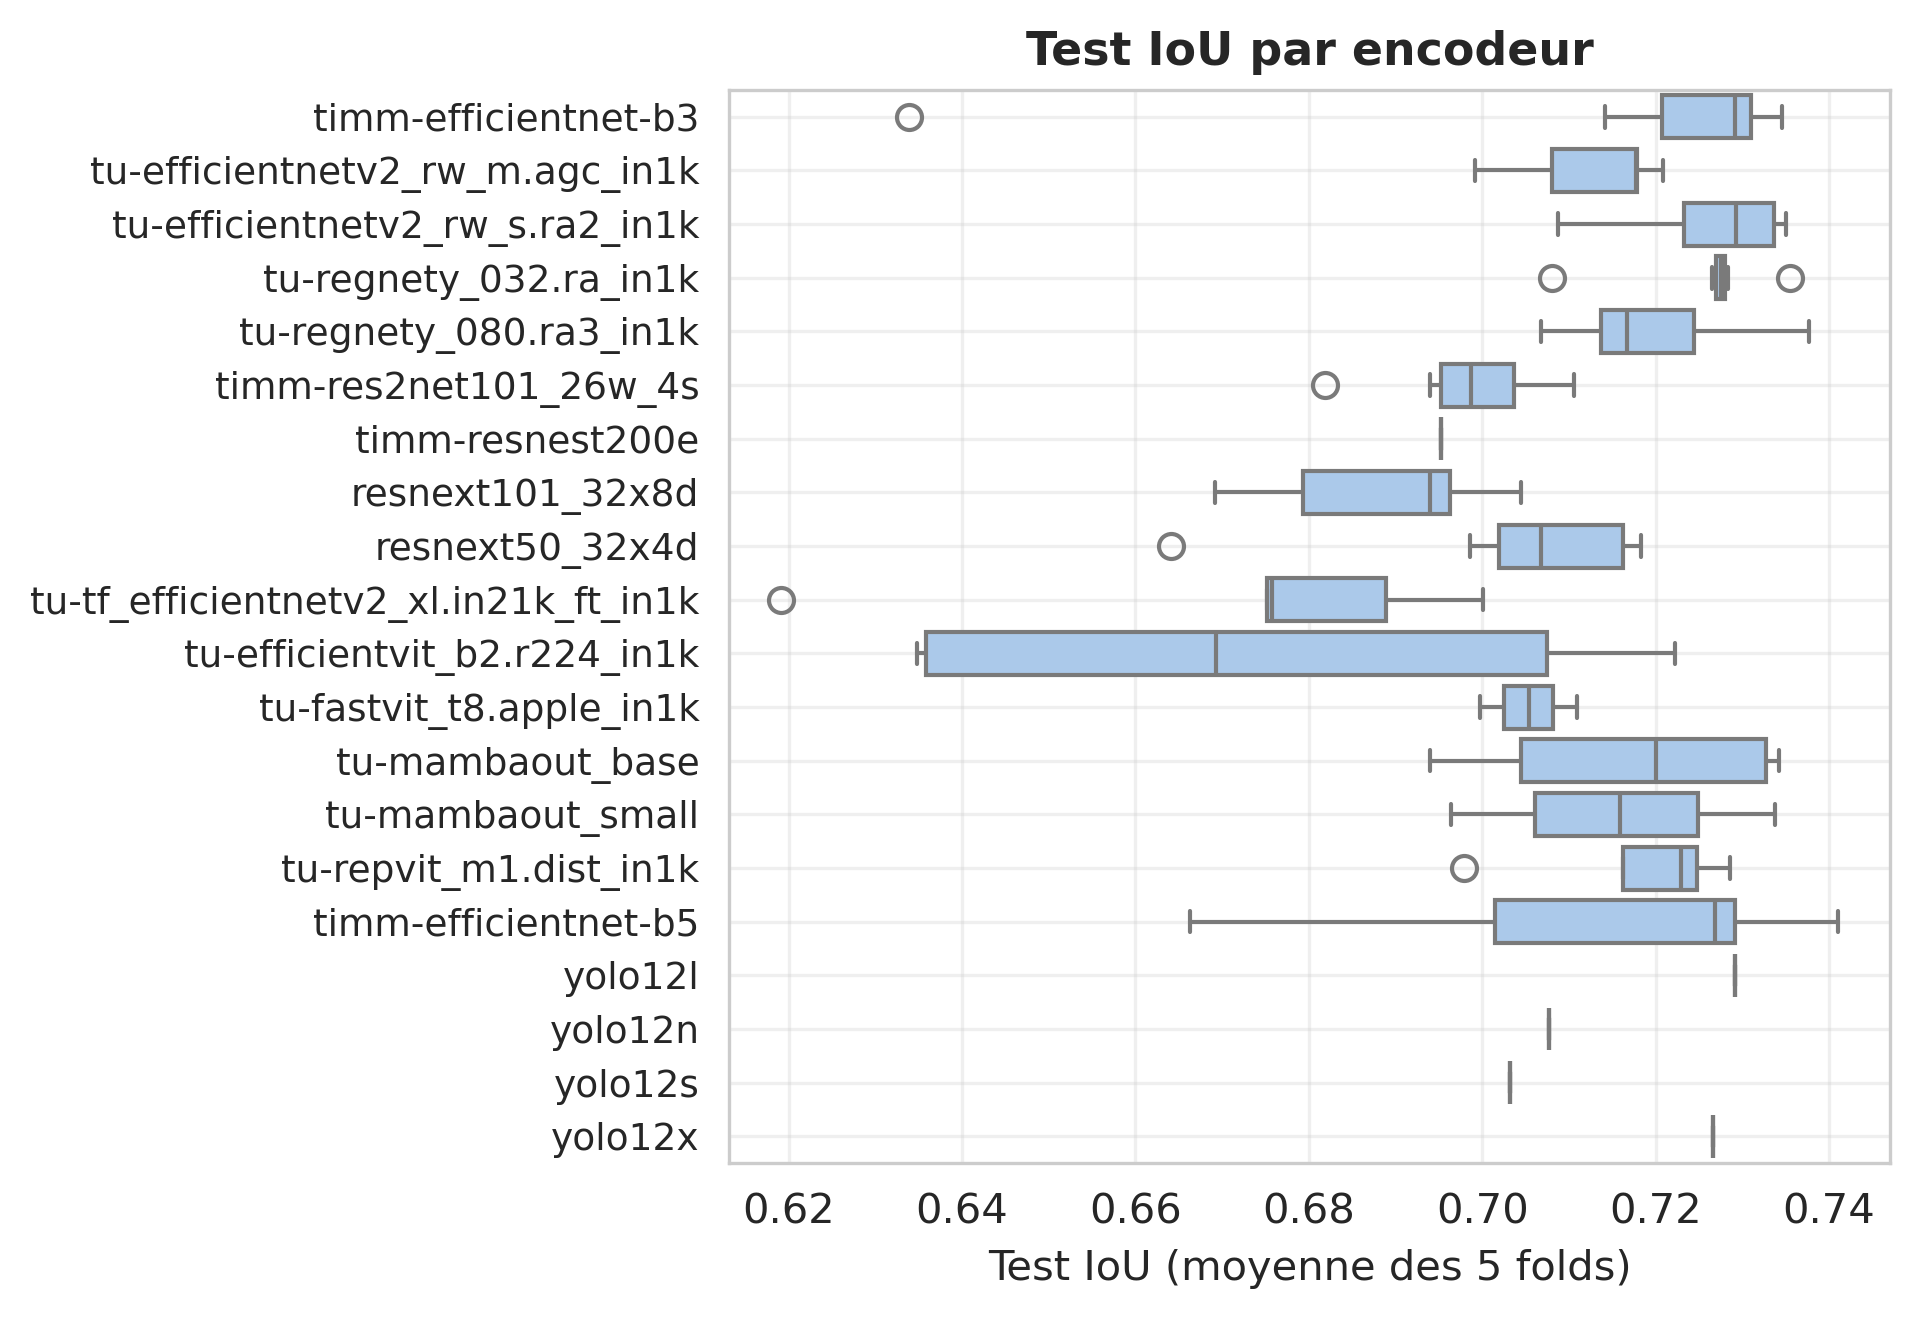
\includegraphics[width=1.20\textwidth]{02-main//figures/ch4/ch4_07_backbone_boxplot_01_eval_test_iou_mean.png}}
    \caption{Boîte à moustaches IoU par encodeur}
    \label{fig:ch4_07_backbone_boxplot_01_eval_test_iou_mean}
\end{figure}

\begin{table}[H]
    \centering
    \begin{tabular}{lrrrrr}
    \toprule
    Encodeur & \multicolumn{5}{c}{IoU} \\
    & Moyenne & écart-type & Médiane & Minimum & Maximum \\
    \midrule
    resnext101 & 0.688 & 0.013 & 0.694 & 0.669 & 0.704 \\
    resnext50 & 0.705 & 0.016 & 0.707 & 0.664 & 0.718 \\
    efficientnet-b3 & 0.714 & 0.036 & 0.729 & 0.634 & 0.735 \\
    efficientnet-b5 & 0.713 & 0.030 & 0.727 & 0.666 & 0.741 \\
    res2net101 & 0.699 & 0.009 & 0.699 & 0.682 & 0.711 \\
    resnest200e & 0.695 &  & 0.695 & 0.695 & 0.695 \\
    efficientnetv2\_rw\_m & 0.713 & 0.009 & 0.718 & 0.699 & 0.721 \\
    efficientnetv2\_rw\_s & 0.727 & 0.008 & 0.729 & 0.709 & 0.735 \\
    efficientvit\_b2 & 0.674 & 0.045 & 0.669 & 0.635 & 0.722 \\
    fastvit\_t8 & 0.705 & 0.008 & 0.705 & 0.700 & 0.711 \\
    mambaout\_base & 0.717 & 0.020 & 0.720 & 0.694 & 0.734 \\
    mambaout\_small & 0.715 & 0.019 & 0.716 & 0.696 & 0.734 \\
    regnety\_032 & 0.726 & 0.008 & 0.728 & 0.708 & 0.735 \\
    regnety\_080 & 0.719 & 0.010 & 0.717 & 0.707 & 0.738 \\
    repvit\_m1 & 0.718 & 0.014 & 0.723 & 0.698 & 0.729 \\
    efficientnetv2\_xl & 0.672 & 0.031 & 0.676 & 0.619 & 0.700 \\
    yolo12l & 0.729 &  & 0.729 & 0.729 & 0.729 \\
    yolo12n & 0.708 &  & 0.708 & 0.708 & 0.708 \\
    yolo12s & 0.703 &  & 0.703 & 0.703 & 0.703 \\
    yolo12x & 0.727 &  & 0.727 & 0.727 & 0.727 \\
    \bottomrule
    \end{tabular}
    \caption{Statistiques IoU par encodeur}
    \label{tab:statistique_par_encodeur_iou}
\end{table}

\begin{figure}[H]
    \centering
    \makebox[\textwidth][c]{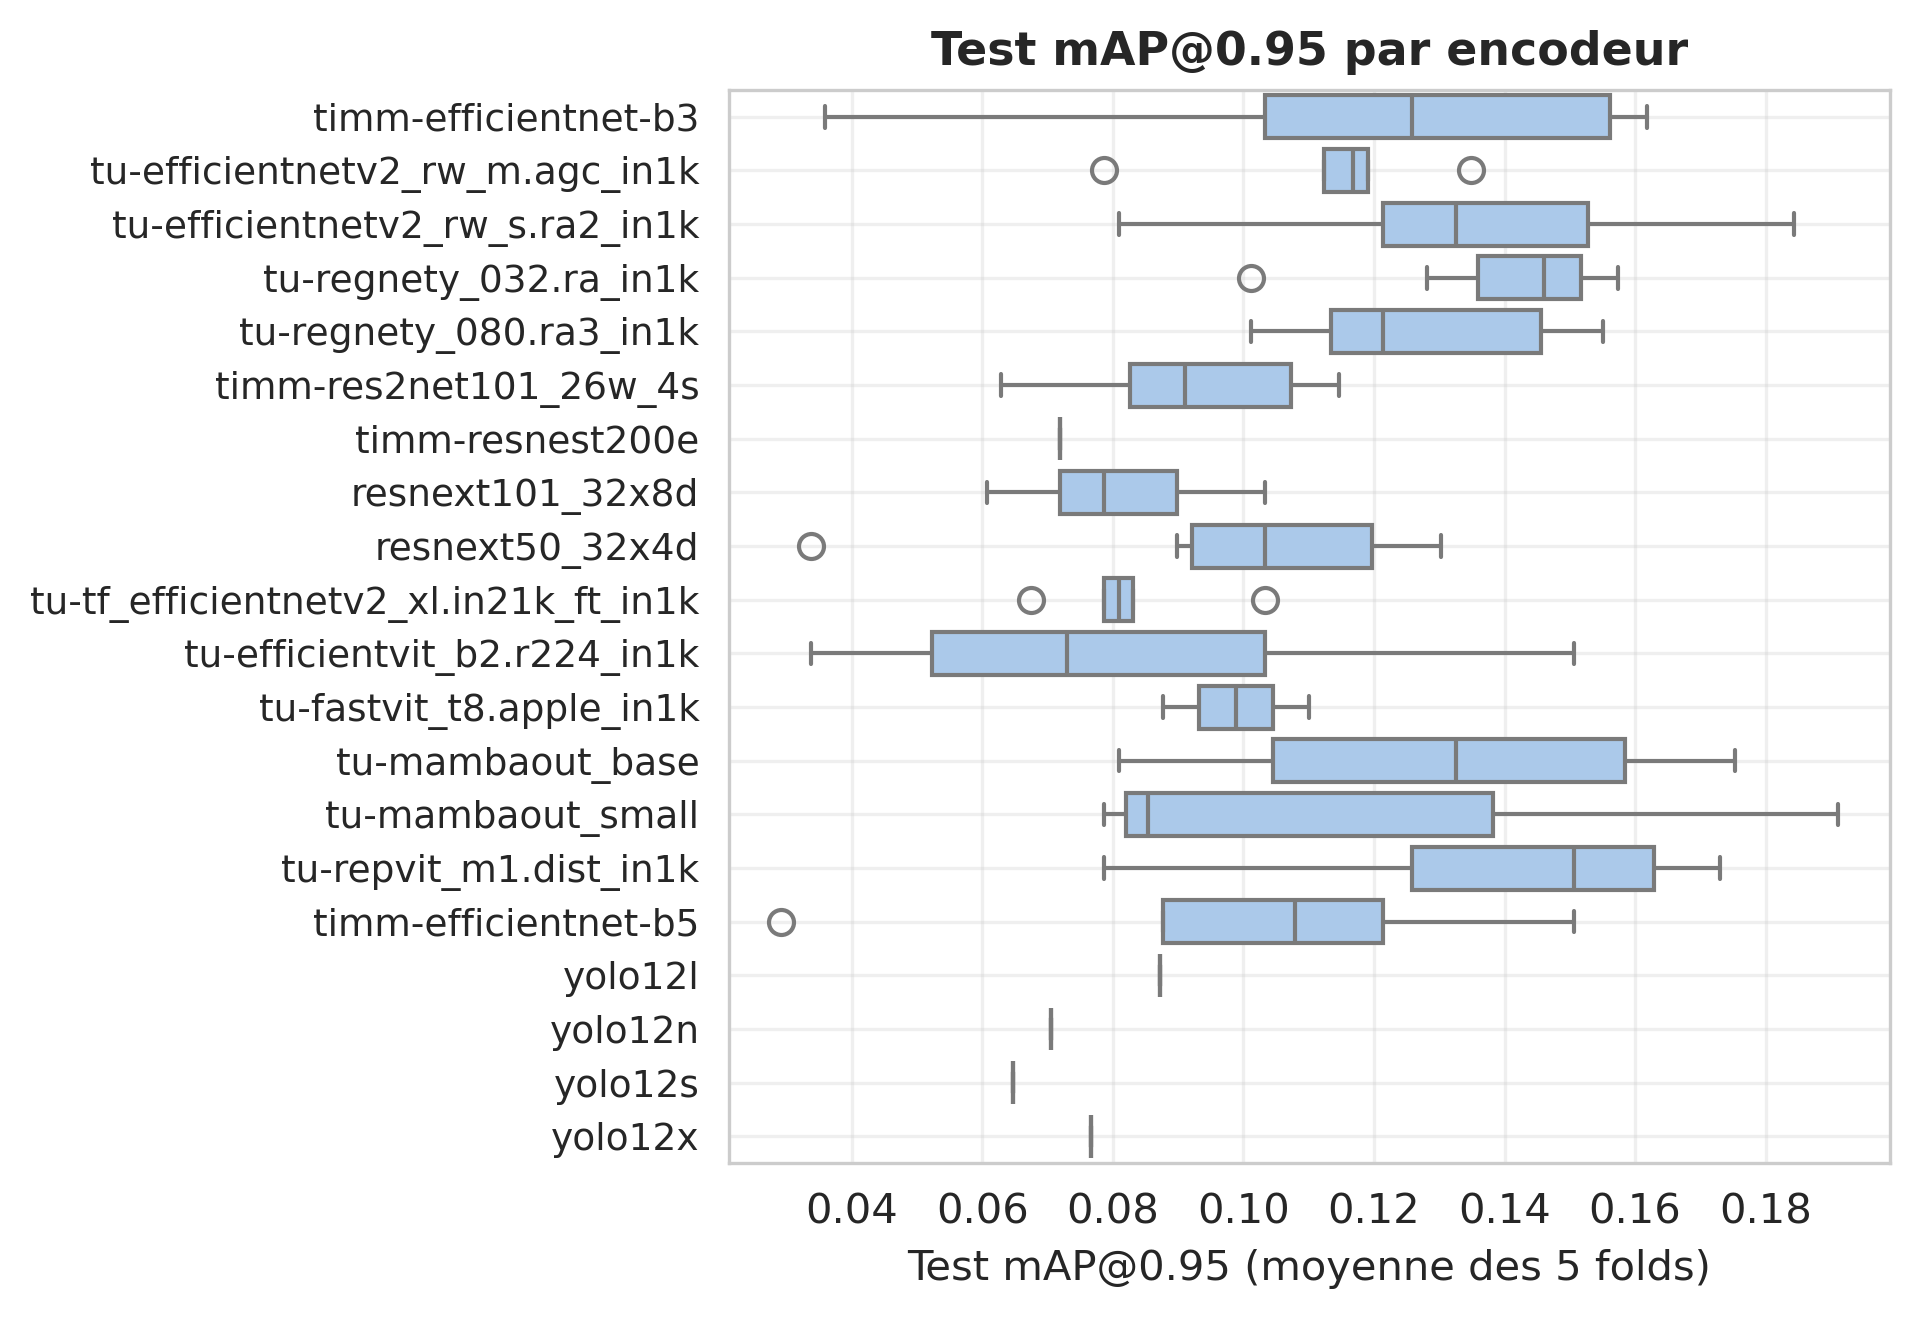
\includegraphics[width=1.20\textwidth]{02-main//figures/ch4/ch4_07_backbone_boxplot_04_eval_test_map_95_mean.png}}
    \caption{Boîte à moustaches IoU par encodeur}
    \label{fig:ch4_07_backbone_boxplot_04_eval_test_map_95_mean}
\end{figure}

\begin{table}[H]
    \centering
    \begin{tabular}{lrrrrr}
    \toprule
    Encodeur & \multicolumn{5}{c}{mAP@0.95} \\
    & Moyenne & écart-type & Médiane & Minimum & Maximum \\
    \midrule
    resnext101 & 0.081 & 0.015 & 0.079 & 0.061 & 0.103 \\
    resnext50 & 0.101 & 0.028 & 0.103 & 0.034 & 0.130 \\
    efficientnet-b3 & 0.120 & 0.045 & 0.126 & 0.036 & 0.162 \\
    efficientnet-b5 & 0.099 & 0.045 & 0.108 & 0.029 & 0.151 \\
    res2net101 & 0.093 & 0.018 & 0.091 & 0.063 & 0.115 \\
    resnest200e & 0.072 &  & 0.072 & 0.072 & 0.072 \\
    efficientnetv2\_rw\_m & 0.112 & 0.021 & 0.117 & 0.079 & 0.135 \\
    efficientnetv2\_rw\_s & 0.136 & 0.030 & 0.133 & 0.081 & 0.184 \\
    efficientvit\_b2 & 0.083 & 0.050 & 0.073 & 0.034 & 0.151 \\
    fastvit\_t8 & 0.099 & 0.016 & 0.099 & 0.088 & 0.110 \\
    mambaout\_base & 0.130 & 0.042 & 0.133 & 0.081 & 0.175 \\
    mambaout\_small & 0.118 & 0.063 & 0.085 & 0.079 & 0.191 \\
    regnety\_032 & 0.140 & 0.019 & 0.146 & 0.101 & 0.157 \\
    regnety\_080 & 0.127 & 0.020 & 0.121 & 0.101 & 0.155 \\
    repvit\_m1 & 0.138 & 0.042 & 0.151 & 0.079 & 0.173 \\
    efficientnetv2\_xl & 0.083 & 0.013 & 0.081 & 0.067 & 0.103 \\
    yolo12l & 0.087 &  & 0.087 & 0.087 & 0.087 \\
    yolo12n & 0.071 &  & 0.071 & 0.071 & 0.071 \\
    yolo12s & 0.065 &  & 0.065 & 0.065 & 0.065 \\
    yolo12x & 0.077 &  & 0.077 & 0.077 & 0.077 \\
    \bottomrule
    \end{tabular}
    \caption{Statistiques mAP@0.95 par décodeur}
    \label{tab:statistique_par_encodeur_map95}
\end{table}

Les encodeurs présentent une variance plus réduite que les décodeurs, témoignant d'une plus grande stabilité des performances. EfficientVIT constitue la seule exception avec une variance importante, probablement liée à sa complexité et à son architecture spécifique.

RepVIT\_M1, EfficientNetV2\_RW\_S et RegNetY\_032 se distinguent par leurs performances élevées, atteignant des IoU moyens respectifs de 0,718, 0,727 et 0,726, ainsi que des mAP@0.95 de 0,138, 0,136 et 0,140.

Les encodeurs mambaout\_base et mambaout\_small affichent également des performances solides avec des IoU moyens de 0,717 et 0,715, accompagnés de mAP@0.95 de 0,130 et 0,118 respectivement. Ces modèles présentent toutefois une variance élevée pour la métrique mAP@0.95, suggérant une compatibilité variable selon les décodeurs associés.


\subsection{Analyse de l'efficacité computationnelle}

\subsubsection{Compromis performance-complexité}

L'analyse du front de Pareto (Figures ~\ref{fig:ch4_09_performance_vs_parameters_pareto_01_eval_test_iou_mean} et \ref{fig:ch4_09_performance_vs_parameters_pareto_04_eval_test_map_95_mean}) identifient les modèles offrant le meilleur compromis entre performance et complexité selon les métriques visées.

\begin{figure}[H]
    \centering
    \makebox[\textwidth][c]{\includegraphics[width=1.05\textwidth]{02-main//figures/ch4/ch4_09_performance_vs_parameters_pareto_01_eval_test_iou_mean.png}}
    \caption{IoU vs nombre de paramètres. Les modèles sur la ligne rouge représentent les solutions optimales.}
    \label{fig:ch4_09_performance_vs_parameters_pareto_01_eval_test_iou_mean}
\end{figure}

Les modèles optimaux identifiés dans la Figure \ref{fig:ch4_09_performance_vs_parameters_pareto_01_eval_test_iou_mean} sont :
\begin{enumerate}
    \item linknet + EfficientNet-B5 (IoU 0,741, 28,75M params)
    \item segformer + RegNetY-032 (IoU 0,735, 18,87M params)
    \item unet++ + EfficientNet-B3 (IoU 0,735, 13,63M params)
\end{enumerate}

Au-delà de 25M paramètres, les gains en IoU deviennent marginaux (<1\% IoU), suggérant une saturation du bénéfice apporté par la complexité additionnelle.

\begin{figure}[H]
    \centering
    \makebox[\textwidth][c]{\includegraphics[width=1.05\textwidth]{02-main//figures/ch4/ch4_09_performance_vs_parameters_pareto_04_eval_test_map_95_mean.png}}
    \caption{mAP@0.95 vs nombre de paramètres. Les modèles sur la ligne rouge représentent les solutions optimales.}
    \label{fig:ch4_09_performance_vs_parameters_pareto_04_eval_test_map_95_mean}
\end{figure}

Les encodeurs (Figure \ref{fig:ch4_09_performance_vs_parameters_pareto_04_eval_test_map_95_mean}) mambaout\_small et EfficientNetV2\_S et les décodeurs PSPNet offrent un bon compromis entre précision de segmentation et complexité. 

\subsubsection{Analyse temporelle}

La distribution des temps d'entraînement (Figure~\ref{fig:ch4_11_training_time_dist_09}) nécessaires révèlent des écarts significatifs entre les modèles, allant de 1,8 à 48,3 heures pour les configurations les plus complexes. Il n'y a pas de corrélation évidente entre le nombre de paramètres et le temps d'entraînement, ce qui suggère que la complexité des architectures joue un rôle plus important que la taille brute du modèle.

\begin{figure}[H]
    \centering
    \includegraphics[width=1\textwidth]{02-main//figures/ch4/ch4_11_training_time_dist_09.png}
    \caption{Distribution du temps d'entraînement total (5 fold)}
    \label{fig:ch4_11_training_time_dist_09}
\end{figure}

\subsection{Analyse des métriques complémentaires}

\subsubsection{Analyse mAP multi-seuils}

Le Tableau~\ref{tab:performance_moyenne_map_different_seuils} présente l'évolution des performances selon différents seuils de mAP.

\begin{table}[H]
    \centering
    \makebox[\textwidth][c]{%
    \begin{tabular}{lrrrrrrr}
    \toprule
    Décodeur & mAP@0.5 & mAP@0.65 & mAP@0.75 & mAP@0.85 & mAP@0.90 & mAP@0.95 & Chute relative \\
    \midrule
    YOLO & 0.577 & 0.468 & 0.378 & 0.279 & 0.189 & 0.075 & -87.0\% \\
    deeplabv3 & 0.834 & 0.725 & 0.604 & 0.416 & 0.265 & 0.110 & -86.8\% \\
    fpn & 0.829 & 0.728 & 0.618 & 0.433 & 0.285 & 0.116 & -86.0\% \\
    linknet & 0.837 & 0.732 & 0.616 & 0.443 & 0.294 & 0.130 & -84.5\% \\
    manet & 0.805 & 0.651 & 0.498 & 0.287 & 0.150 & 0.062 & -92.3\% \\
    pan & 0.814 & 0.702 & 0.584 & 0.401 & 0.254 & 0.096 & -88.2\% \\
    pspnet & 0.827 & 0.705 & 0.588 & 0.387 & 0.243 & 0.087 & -89.5\% \\
    segformer & 0.829 & 0.738 & 0.628 & 0.444 & 0.298 & 0.131 & -84.2\% \\
    unet & 0.834 & 0.731 & 0.615 & 0.429 & 0.283 & 0.128 & -84.7\% \\
    unetplusplus & 0.837 & 0.719 & 0.594 & 0.406 & 0.255 & 0.107 & -87.2\% \\
    upernet & 0.837 & 0.745 & 0.635 & 0.459 & 0.313 & 0.137 & -83.6\% \\
    \bottomrule
    \end{tabular}%
    }
    \caption{Performances moyennes mAP à différents seuils. Chute relative mAP@0.5 à mAP@0.95}
    \label{tab:performance_moyenne_map_different_seuils}
\end{table}

Les modèles SMP conservent mieux leurs performances aux seuils élevés, à l'exception de MANet, démontrant une segmentation plus précise des contours. La transition du mAP@0.5 au mAP@0.95 révèle une chute significative des performances, pouvant atteindre jusqu'à -92,3\% pour MANet. Les modèles UNet et UPerNet présentent des diminutions plus modérées de -84,7\% et -83,6\% respectivement, suggérant une robustesse relative face aux seuils exigeants.

L'analyse du passage de mAP@0.90 à mAP@0.95 met en évidence une dégradation importante des performances, dépassant 50\% dans tous les cas. Cette observation souligne la difficulté intrinsèque à maintenir une précision élevée dans les détections les plus exigeantes.

\subsection{Analyse par catégorie de taille}

L'analyse des performances selon la taille des modèles (Figures ~\ref{fig:ch4_05_models_by_size_category_01_eval_test_iou_mean} et \ref{fig:ch4_05_models_by_size_category_04_eval_test_map_95_mean}) met en évidence plusieurs points intéressants.

Les deux métriques utilisées montrent des résultats assez différents. Pour l'IoU (Figure \ref{fig:ch4_05_models_by_size_category_01_eval_test_iou_mean}), les performances restent relativement stables peu importe la taille du modèle, avec des valeurs comprises entre 0,689 et 0,741. Cette constance indique que le nombre de paramètres n'influence pas directement la qualité de segmentation.

\begin{figure}[H]
    \centering
    \makebox[\textwidth][c]{\includegraphics[width=1.05\textwidth]{02-main//figures/ch4/ch4_05_models_by_size_category_01_eval_test_iou_mean.png}}
    \caption{Top 3 modèles par IoU par taille (paramètres)}
    \label{fig:ch4_05_models_by_size_category_01_eval_test_iou_mean}
\end{figure}

Des modèles légers comme RepViT avec seulement 7M de paramètres obtiennent des résultats similaires à des architectures plus lourdes comme MambaOut qui en compte 101M. Cela montre que des approches bien optimisées peuvent être très efficaces pour segmenter les toitures.

La métrique mAP@0.95 (Figure \ref{fig:ch4_05_models_by_size_category_04_eval_test_map_95_mean}) raconte une histoire différente. Cette métrique, qui mesure la précision avec un seuil IoU strict de 0.95, donne des résultats plus variés allant de 0,083 à 0,191. Les écarts sont donc beaucoup plus marqués entre les différentes architectures.

\begin{figure}[H]
    \centering
    \makebox[\textwidth][c]{\includegraphics[width=1.05\textwidth]{02-main//figures/ch4/ch4_05_models_by_size_category_04_eval_test_map_95_mean.png}}
    \caption{Top 3 modèles par mAP@0.95 par taille (paramètres)}
    \label{fig:ch4_05_models_by_size_category_04_eval_test_map_95_mean}
\end{figure}

Un résultat surprenant est que les modèles de taille moyenne (25-50M paramètres) obtiennent les meilleurs scores mAP@0.95. Ce n'est donc pas une simple relation où plus gros égale meilleur - il semble y avoir une taille optimale qui balance capacité de représentation et efficacité d'apprentissage.

Un autre point important concerne l'architecture elle-même. En prenant l'exemple d'EfficientNet, on constate que selon le décodeur utilisé (UNet, SegFormer ou FPN), les performances peuvent varier significativement même si la taille reste similaire. Le choix du décodeur est donc tout aussi important que celui de l'encodeur pour obtenir de bons résultats en segmentation.

\subsection{Analyse qualitative}
Cette sous-section examine des exemples concrets de segmentation produits par les modèles ayant obtenu les meilleures performances.

\subsubsection{Modèles retenus}
La sélection des modèles s'est basée sur leurs performances sur le dataset de test selon plusieurs métriques : IoU, mAP@0.5, mAP@0.75, mAP@0.95 et F1-score. Les combinaisons encodeur-décodeur retenues sont :
\begin{itemize}
    \item UNet + mambaout\_small
    \item UPerNet + EfficientNetV2-S
    \item Segformer + mambaout\_base
    \item LinkNet + EfficientNet-B5
    \item Unet++ + EfficientNetV2-S
    \item SegFormer + RegNetY-080
\end{itemize}

Pour chaque combinaison, 5 modèles ont été entraînés suivant la méthode de validation croisée. Chaque modèle utilise un fold différent pour la validation et les quatre autres pour l'entraînement. Il faut donc déterminer comment combiner efficacement les prédictions de ces 5 modèles pour obtenir un résultat final.

\subsubsection{Stratégie d'ensemble k-fold}

L'approche retenue consiste à exploiter la complémentarité des modèles issus de la validation croisée. Plutôt que de sélectionner le meilleur modèle parmi les 5 folds de chaque combinaison, les prédictions des 5 modèles sont combinées. Cette stratégie d'ensemble permet d'obtenir des segmentations plus robustes et moins sensibles aux variations dans les données d'entraînement.

\paragraph{Principe de fonctionnement}

Pour chaque combinaison encodeur-décodeur, voici comment se déroule le processus :

\begin{enumerate}
    \item Récupération des modèles : Les 5 modèles entraînés sont chargés un par un pour éviter de saturer la mémoire GPU
    \item Prédiction individuelle : Chaque modèle produit une carte de probabilité pour toutes les images du dataset de test
    \item Agrégation des prédictions : Les probabilités sont moyennées pixel par pixel avec la formule suivante :
    \vspace{0.45cm}
    \begin{equation}
        P_{ensemble}(x,y) = \frac{1}{K} \sum_{k=1}^{K} P_k(x,y)
    \end{equation}
    où $K=5$ correspond au nombre de folds et $P_k(x,y)$ représente la probabilité donnée par le modèle du fold $k$ au pixel $(x,y)$
    \item Binarisation : Les probabilités moyennées sont transformées en masque binaire en appliquant un seuil de 0.5
\end{enumerate}

\paragraph{Avantages de l'approche}

Cette stratégie d'ensemble apporte plusieurs avantages :

\begin{itemize}
    \item Réduction de la variance : La moyenne des prédictions de modèles entraînés sur différents sous-ensembles diminue la sensibilité aux variations aléatoires dans les données
    \item Amélioration de la généralisation : Comme chaque modèle a vu des données de validation différentes, l'ensemble obtient une vue plus complète du problème
    \item Robustesse accrue : Les erreurs des modèles individuels ont tendance à se compenser lors de l'agrégation, ce qui limite l'impact des prédictions aberrantes
    \item Exploitation maximale des données : Avec 5 folds, chaque échantillon participe à l'entraînement de 4 modèles sur 5
\end{itemize}

\paragraph{Inconvénients et limitations}

Cette approche présente aussi quelques contraintes :

\begin{itemize}
    \item Coût computationnel : L'inférence prend 5 fois plus de temps, passant de quelques secondes à plusieurs dizaines de secondes par image
    \item Consommation mémoire : Même si les modèles sont chargés un par un, stocker 5 modèles par configuration demande environ 5 fois plus d'espace disque
    \item Complexité de déploiement : Gérer plusieurs modèles rend le système plus complexe à mettre en production
\end{itemize}

\paragraph{Optimisations techniques}

Pour limiter les problèmes de mémoire, plusieurs stratégies ont été mises en place :

\begin{itemize}
    \item Chargement séquentiel des modèles avec libération de la mémoire GPU après chaque fold (\texttt{torch.cuda.empty\_cache()})
    \item Traitement par batch des images pour rentabiliser le chargement des modèles
    \item Accumulation progressive des prédictions pour éviter de garder toutes les probabilités en mémoire en même temps
\end{itemize}

Cette approche d'ensemble k-fold offre un bon équilibre entre précision et efficacité. Elle convient particulièrement aux cas où la qualité des résultats est plus importante que la vitesse de traitement.

\paragraph{Résultats de l'ensemble k-fold}

Le Tableau \ref{tab:kfold_ensemble} présente les performances des modèles avec et sans ensemble k-fold. Les résultats montrent que l'ensemble est plus performant que la moyenne des folds de chaque modèle.

\begin{table}[H]
    \centering
    \makebox[\textwidth][c]{%
    \begin{tabular}{lccccc}
    \toprule
    Modèle & Folds & Moy. fold IoU & Meilleur fold IoU & Ensemble IoU & Amélioration \\
    \midrule
    UNet + mambaout\_small & 5 & 0.734 $\pm$ 0.012 & 0.748 & \textbf{0.745} & +1.6\% \\
    UPerNet + EfficientNetV2-S & 5 & 0.735 $\pm$ 0.005 & 0.743 & \textbf{0.748} & +1.8\% \\
    Segformer + mambaout\_base & 5 & 0.734 $\pm$ 0.009 & 0.747 & \textbf{0.742} & +1.0\% \\
    LinkNet + EfficientNet-B5 & 5 & 0.741 $\pm$ 0.003 & 0.744 & \textbf{0.752} & +1.5\% \\
    Unet++ + EfficientNetV2-S & 5 & 0.723 $\pm$ 0.012 & 0.738 & \textbf{0.737} & +2.0\% \\
    SegFormer + RegNetY-080 & 5 & 0.738 $\pm$ 0.006 & 0.746 & \textbf{0.745} & +0.9\% \\
    \bottomrule
    \end{tabular}%
    }
    \caption{Comparaison des performances des modèles avec et sans ensemble k-fold. Amélioration calculée par rapport à l'IoU moyen des folds.}
    \label{tab:kfold_ensemble}
\end{table}

\subsubsection{Visualisation des résultats}

Les figures \ref{fig:unet_mambaoutsmall_best_cases} et \ref{fig:unet_mambaoutsmall_worst_cases} illustrent les cas extrêmes de performance du modèle UNet avec mambaout\_small sur le dataset de test.

La Figure \ref{fig:unet_mambaoutsmall_best_cases} montre les 4 segmentations les plus réussies avec des valeurs IoU élevées. Le modèle parvient à identifier correctement les toitures dans diverses situations. Les résultats montrent que même les obstacles de petite taille comme les cheminées sont correctement détectés, ce qui indique une bonne capacité de segmentation fine.

La Figure \ref{fig:unet_mambaoutsmall_worst_cases} présente les 4 cas les plus problématiques avec des IoU très bas. Les erreurs se concentrent sur les toitures végétalisées et les terrasses praticables, révélant les difficultés du modèle à traiter ces types de surfaces particulières.

% =========================================================

\begin{figure}[H]
\centering
\begin{subfigure}{0.32\textwidth}
    \includegraphics[width=\textwidth]{02-main//figures/ch4/kfold_ensembles/unet_tu-mambaout_small/best_cases/best_5_iou0.998_24991116_tile_5_3_322356_original.png}
    \caption{Top1 - Original}
\end{subfigure}
\hfill
\begin{subfigure}{0.32\textwidth}
    \includegraphics[width=\textwidth]{02-main//figures/ch4/kfold_ensembles/unet_tu-mambaout_small/best_cases/best_5_iou0.998_24991116_tile_5_3_322356_overlay_gt.png}
    \caption{Vérité terrain}
\end{subfigure}
\hfill
\begin{subfigure}{0.32\textwidth}
    \includegraphics[width=\textwidth]{02-main//figures/ch4/kfold_ensembles/unet_tu-mambaout_small/best_cases/best_5_iou0.998_24991116_tile_5_3_322356_overlay_pred.png}
    \caption{Prédiction - IoU = 0.998}
\end{subfigure}

\vspace{0.35cm}

\begin{subfigure}{0.32\textwidth}
    \includegraphics[width=\textwidth]{02-main//figures/ch4/kfold_ensembles/unet_tu-mambaout_small/best_cases/best_4_iou0.991_24961121_tile_15_10_cc6553_original.png}
    \caption{Top2 - Original}
\end{subfigure}
\hfill
\begin{subfigure}{0.32\textwidth}
    \includegraphics[width=\textwidth]{02-main//figures/ch4/kfold_ensembles/unet_tu-mambaout_small/best_cases/best_4_iou0.991_24961121_tile_15_10_cc6553_overlay_gt.png}
    \caption{Vérité terrain}
\end{subfigure}
\hfill
\begin{subfigure}{0.32\textwidth}
    \includegraphics[width=\textwidth]{02-main//figures/ch4/kfold_ensembles/unet_tu-mambaout_small/best_cases/best_4_iou0.991_24961121_tile_15_10_cc6553_overlay_pred.png}
    \caption{Prédiction - IoU = 0.991}
\end{subfigure}

\vspace{0.35cm}

\begin{subfigure}{0.32\textwidth}
    \includegraphics[width=\textwidth]{02-main//figures/ch4/kfold_ensembles/unet_tu-mambaout_small/best_cases/best_3_iou0.988_24931117_tile_18_5_f475a0_original.png}
    \caption{Top3 - Original}
\end{subfigure}
\hfill
\begin{subfigure}{0.32\textwidth}
    \includegraphics[width=\textwidth]{02-main//figures/ch4/kfold_ensembles/unet_tu-mambaout_small/best_cases/best_3_iou0.988_24931117_tile_18_5_f475a0_overlay_gt.png}
    \caption{Vérité terrain}
\end{subfigure}
\hfill
\begin{subfigure}{0.32\textwidth}
    \includegraphics[width=\textwidth]{02-main//figures/ch4/kfold_ensembles/unet_tu-mambaout_small/best_cases/best_3_iou0.988_24931117_tile_18_5_f475a0_overlay_pred.png}
    \caption{Prédiction - IoU = 0.988}
\end{subfigure}

\vspace{0.35cm}

\begin{subfigure}{0.32\textwidth}
    \includegraphics[width=\textwidth]{02-main//figures/ch4/kfold_ensembles/unet_tu-mambaout_small/best_cases/best_2_iou0.984_24931113_tile_13_18_a66e08_original.png}
    \caption{Top4 - Original}
\end{subfigure}
\hfill
\begin{subfigure}{0.32\textwidth}
    \includegraphics[width=\textwidth]{02-main//figures/ch4/kfold_ensembles/unet_tu-mambaout_small/best_cases/best_2_iou0.984_24931113_tile_13_18_a66e08_overlay_gt.png}
    \caption{Vérité terrain}
\end{subfigure}
\hfill
\begin{subfigure}{0.32\textwidth}
    \includegraphics[width=\textwidth]{02-main//figures/ch4/kfold_ensembles/unet_tu-mambaout_small/best_cases/best_2_iou0.984_24931113_tile_13_18_a66e08_overlay_pred.png}
    \caption{Prédiction - IoU = 0.984}
\end{subfigure}

\caption{Meilleurs IoU pour Unet avec mambaout\_small backbone sur le dataset de test}
\label{fig:unet_mambaoutsmall_best_cases}
\end{figure}

% =========================================================

\begin{figure}[H]
\centering
\begin{subfigure}{0.32\textwidth}
    \includegraphics[width=\textwidth]{02-main//figures/ch4/kfold_ensembles/unet_tu-mambaout_small/worst_cases/worst_5_iou0.000_25001117_tile_3_9_5ba8f7_original.png}
    \caption{Top1 - Original}
\end{subfigure}
\hfill
\begin{subfigure}{0.32\textwidth}
    \includegraphics[width=\textwidth]{02-main//figures/ch4/kfold_ensembles/unet_tu-mambaout_small/worst_cases/worst_5_iou0.000_25001117_tile_3_9_5ba8f7_overlay_gt.png}
    \caption{Vérité terrain}
\end{subfigure}
\hfill
\begin{subfigure}{0.32\textwidth}
    \includegraphics[width=\textwidth]{02-main//figures/ch4/kfold_ensembles/unet_tu-mambaout_small/worst_cases/worst_5_iou0.000_25001117_tile_3_9_5ba8f7_overlay_pred.png}
    \caption{Prédiction - IoU = 0.000}
\end{subfigure}

\vspace{0.35cm}

\begin{subfigure}{0.32\textwidth}
    \includegraphics[width=\textwidth]{02-main//figures/ch4/kfold_ensembles/unet_tu-mambaout_small/worst_cases/worst_4_iou0.000_25001112_tile_9_1_991a94_original.png}
    \caption{Top2 - Original}
\end{subfigure}
\hfill
\begin{subfigure}{0.32\textwidth}
    \includegraphics[width=\textwidth]{02-main//figures/ch4/kfold_ensembles/unet_tu-mambaout_small/worst_cases/worst_4_iou0.000_25001112_tile_9_1_991a94_overlay_gt.png}
    \caption{Vérité terrain}
\end{subfigure}
\hfill
\begin{subfigure}{0.32\textwidth}
    \includegraphics[width=\textwidth]{02-main//figures/ch4/kfold_ensembles/unet_tu-mambaout_small/worst_cases/worst_4_iou0.000_25001112_tile_9_1_991a94_overlay_pred.png}
    \caption{Prédiction - IoU = 0.000}
\end{subfigure}

\vspace{0.35cm}

\begin{subfigure}{0.32\textwidth}
    \includegraphics[width=\textwidth]{02-main//figures/ch4/kfold_ensembles/unet_tu-mambaout_small/worst_cases/worst_3_iou0.000_24991122_tile_9_19_7ebcec_original.png}
    \caption{Top3 - Original}
\end{subfigure}
\hfill
\begin{subfigure}{0.32\textwidth}
    \includegraphics[width=\textwidth]{02-main//figures/ch4/kfold_ensembles/unet_tu-mambaout_small/worst_cases/worst_3_iou0.000_24991122_tile_9_19_7ebcec_overlay_gt.png}
    \caption{Vérité terrain}
\end{subfigure}
\hfill
\begin{subfigure}{0.32\textwidth}
    \includegraphics[width=\textwidth]{02-main//figures/ch4/kfold_ensembles/unet_tu-mambaout_small/worst_cases/worst_3_iou0.000_24991122_tile_9_19_7ebcec_overlay_pred.png}
    \caption{Prédiction - IoU = 0.000}
\end{subfigure}

\vspace{0.35cm}

\begin{subfigure}{0.32\textwidth}
    \includegraphics[width=\textwidth]{02-main//figures/ch4/kfold_ensembles/unet_tu-mambaout_small/worst_cases/worst_2_iou0.000_24951112_tile_4_13_2bd653_original.png}
    \caption{Top4 - Original}
\end{subfigure}
\hfill
\begin{subfigure}{0.32\textwidth}
    \includegraphics[width=\textwidth]{02-main//figures/ch4/kfold_ensembles/unet_tu-mambaout_small/worst_cases/worst_2_iou0.000_24951112_tile_4_13_2bd653_overlay_gt.png}
    \caption{Vérité terrain}
\end{subfigure}
\hfill
\begin{subfigure}{0.32\textwidth}
    \includegraphics[width=\textwidth]{02-main//figures/ch4/kfold_ensembles/unet_tu-mambaout_small/worst_cases/worst_2_iou0.000_24951112_tile_4_13_2bd653_overlay_pred.png}
    \caption{Prédiction - IoU = 0.000}
\end{subfigure}

\caption{Pires IoU pour Unet avec mambaout\_small sur le dataset de test}
\label{fig:unet_mambaoutsmall_worst_cases}
\end{figure}

% =========================================================

Les Figures \ref{fig:upernet_efficientnetv2_s_best_cases} et \ref{fig:upernet_efficientnetv2_s_best_cases} illustrent les performances extrêmes du modèle UPerNet + EfficientNetV2\_RW\_S sur le dataset de test.

La Figure \ref{fig:upernet_efficientnetv2_s_best_cases} présente les 4 meilleures segmentations. Les résultats sont proches de ceux obtenus avec UNet + mambaout\_small - trois images sur quatre sont identiques à celles de la Figure \ref{fig:unet_mambaoutsmall_best_cases}.

La Figure \ref{fig:upernet_efficientnetv2_s_best_cases} montre les 4 pires cas. Là aussi, on retrouve trois images communes avec la Figure \ref{fig:unet_mambaoutsmall_worst_cases}, confirmant que les deux modèles peinent sur les mêmes types de surfaces (toitures végétalisées et terrasses praticables). La quatrième image présente une toiture de type hangar où la vérité terrain semble questionnable, les critères de labellisation pourraient ne pas être adaptés à ce cas particulier.


\begin{figure}[H]
\centering
\begin{subfigure}{0.32\textwidth}
    \includegraphics[width=\textwidth]{02-main//figures/ch4/kfold_ensembles/upernet_tu-efficientnetv2_rw_s.ra2_in1k/best_cases/best_5_iou0.999_24991116_tile_5_3_322356_original.png}
    \caption{Top1 - Original}
\end{subfigure}
\hfill
\begin{subfigure}{0.32\textwidth}
    \includegraphics[width=\textwidth]{02-main//figures/ch4/kfold_ensembles/upernet_tu-efficientnetv2_rw_s.ra2_in1k/best_cases/best_5_iou0.999_24991116_tile_5_3_322356_overlay_gt.png}
    \caption{Vérité terrain}
\end{subfigure}
\hfill
\begin{subfigure}{0.32\textwidth}
    \includegraphics[width=\textwidth]{02-main//figures/ch4/kfold_ensembles/upernet_tu-efficientnetv2_rw_s.ra2_in1k/best_cases/best_5_iou0.999_24991116_tile_5_3_322356_overlay_pred.png}
    \caption{Prédiction - IoU = 0.999}
\end{subfigure}

\vspace{0.35cm}

\begin{subfigure}{0.32\textwidth}
    \includegraphics[width=\textwidth]{02-main//figures/ch4/kfold_ensembles/upernet_tu-efficientnetv2_rw_s.ra2_in1k/best_cases/best_4_iou0.987_24961121_tile_15_10_cc6553_original.png}
    \caption{Top2 - Original}
\end{subfigure}
\hfill
\begin{subfigure}{0.32\textwidth}
    \includegraphics[width=\textwidth]{02-main//figures/ch4/kfold_ensembles/upernet_tu-efficientnetv2_rw_s.ra2_in1k/best_cases/best_4_iou0.987_24961121_tile_15_10_cc6553_overlay_gt.png}
    \caption{Vérité terrain}
\end{subfigure}
\hfill
\begin{subfigure}{0.32\textwidth}
    \includegraphics[width=\textwidth]{02-main//figures/ch4/kfold_ensembles/upernet_tu-efficientnetv2_rw_s.ra2_in1k/best_cases/best_4_iou0.987_24961121_tile_15_10_cc6553_overlay_pred.png}
    \caption{Prédiction - IoU = 0.987}
\end{subfigure}

\vspace{0.35cm}

\begin{subfigure}{0.32\textwidth}
    \includegraphics[width=\textwidth]{02-main//figures/ch4/kfold_ensembles/upernet_tu-efficientnetv2_rw_s.ra2_in1k/best_cases/best_3_iou0.987_24941121_tile_16_8_fd3555_original.png}
    \caption{Top3 - Original}
\end{subfigure}
\hfill
\begin{subfigure}{0.32\textwidth}
    \includegraphics[width=\textwidth]{02-main//figures/ch4/kfold_ensembles/upernet_tu-efficientnetv2_rw_s.ra2_in1k/best_cases/best_3_iou0.987_24941121_tile_16_8_fd3555_overlay_gt.png}
    \caption{Vérité terrain}
\end{subfigure}
\hfill
\begin{subfigure}{0.32\textwidth}
    \includegraphics[width=\textwidth]{02-main//figures/ch4/kfold_ensembles/upernet_tu-efficientnetv2_rw_s.ra2_in1k/best_cases/best_3_iou0.987_24941121_tile_16_8_fd3555_overlay_pred.png}
    \caption{Prédiction - IoU = 0.987}
\end{subfigure}

\vspace{0.35cm}

\begin{subfigure}{0.32\textwidth}
    \includegraphics[width=\textwidth]{02-main//figures/ch4/kfold_ensembles/upernet_tu-efficientnetv2_rw_s.ra2_in1k/best_cases/best_2_iou0.984_24931113_tile_13_18_a66e08_original.png}
    \caption{Top4 - Original}
\end{subfigure}
\hfill
\begin{subfigure}{0.32\textwidth}
    \includegraphics[width=\textwidth]{02-main//figures/ch4/kfold_ensembles/upernet_tu-efficientnetv2_rw_s.ra2_in1k/best_cases/best_2_iou0.984_24931113_tile_13_18_a66e08_overlay_gt.png}
    \caption{Vérité terrain}
\end{subfigure}
\hfill
\begin{subfigure}{0.32\textwidth}
    \includegraphics[width=\textwidth]{02-main//figures/ch4/kfold_ensembles/upernet_tu-efficientnetv2_rw_s.ra2_in1k/best_cases/best_2_iou0.984_24931113_tile_13_18_a66e08_overlay_pred.png}
    \caption{Prédiction - IoU = 0.984}
\end{subfigure}

\caption{Meilleurs IoU pour UPerNet avec EfficientNetV2-S sur le dataset de test}
\label{fig:upernet_efficientnetv2_s_best_cases}
\end{figure}

% =========================================================

\begin{figure}[H]
\centering
\begin{subfigure}{0.32\textwidth}
    \includegraphics[width=\textwidth]{02-main//figures/ch4/kfold_ensembles/upernet_tu-efficientnetv2_rw_s.ra2_in1k/worst_cases/worst_5_iou0.000_25001117_tile_3_9_5ba8f7_original.png}
    \caption{Top1 - Original}
\end{subfigure}
\hfill
\begin{subfigure}{0.32\textwidth}
    \includegraphics[width=\textwidth]{02-main//figures/ch4/kfold_ensembles/upernet_tu-efficientnetv2_rw_s.ra2_in1k/worst_cases/worst_5_iou0.000_25001117_tile_3_9_5ba8f7_overlay_gt.png}
    \caption{Vérité terrain}
\end{subfigure}
\hfill
\begin{subfigure}{0.32\textwidth}
    \includegraphics[width=\textwidth]{02-main//figures/ch4/kfold_ensembles/upernet_tu-efficientnetv2_rw_s.ra2_in1k/worst_cases/worst_5_iou0.000_25001117_tile_3_9_5ba8f7_overlay_pred.png}
    \caption{Prédiction - IoU = 0.000}
\end{subfigure}

\vspace{0.35cm}

\begin{subfigure}{0.32\textwidth}
    \includegraphics[width=\textwidth]{02-main//figures/ch4/kfold_ensembles/upernet_tu-efficientnetv2_rw_s.ra2_in1k/worst_cases/worst_4_iou0.000_25001112_tile_9_1_991a94_original.png}
    \caption{Top2 - Original}
\end{subfigure}
\hfill
\begin{subfigure}{0.32\textwidth}
    \includegraphics[width=\textwidth]{02-main//figures/ch4/kfold_ensembles/upernet_tu-efficientnetv2_rw_s.ra2_in1k/worst_cases/worst_4_iou0.000_25001112_tile_9_1_991a94_overlay_gt.png}
    \caption{Vérité terrain}
\end{subfigure}
\hfill
\begin{subfigure}{0.32\textwidth}
    \includegraphics[width=\textwidth]{02-main//figures/ch4/kfold_ensembles/upernet_tu-efficientnetv2_rw_s.ra2_in1k/worst_cases/worst_4_iou0.000_25001112_tile_9_1_991a94_overlay_pred.png}
    \caption{Prédiction - IoU = 0.000}
\end{subfigure}

\vspace{0.35cm}

\begin{subfigure}{0.32\textwidth}
    \includegraphics[width=\textwidth]{02-main//figures/ch4/kfold_ensembles/upernet_tu-efficientnetv2_rw_s.ra2_in1k/worst_cases/worst_3_iou0.000_24991122_tile_9_19_7ebcec_original.png}
    \caption{Top3 - Original}
\end{subfigure}
\hfill
\begin{subfigure}{0.32\textwidth}
    \includegraphics[width=\textwidth]{02-main//figures/ch4/kfold_ensembles/upernet_tu-efficientnetv2_rw_s.ra2_in1k/worst_cases/worst_3_iou0.000_24991122_tile_9_19_7ebcec_overlay_gt.png}
    \caption{Vérité terrain}
\end{subfigure}
\hfill
\begin{subfigure}{0.32\textwidth}
    \includegraphics[width=\textwidth]{02-main//figures/ch4/kfold_ensembles/upernet_tu-efficientnetv2_rw_s.ra2_in1k/worst_cases/worst_3_iou0.000_24991122_tile_9_19_7ebcec_overlay_pred.png}
    \caption{Prédiction - IoU = 0.000}
\end{subfigure}

\vspace{0.35cm}

\begin{subfigure}{0.32\textwidth}
    \includegraphics[width=\textwidth]{02-main//figures/ch4/kfold_ensembles/upernet_tu-efficientnetv2_rw_s.ra2_in1k/worst_cases/worst_1_iou0.000_24931113_tile_19_19_52ccbb_original.png}
    \caption{Top4 - Original}
\end{subfigure}
\hfill
\begin{subfigure}{0.32\textwidth}
    \includegraphics[width=\textwidth]{02-main//figures/ch4/kfold_ensembles/upernet_tu-efficientnetv2_rw_s.ra2_in1k/worst_cases/worst_1_iou0.000_24931113_tile_19_19_52ccbb_overlay_gt.png}
    \caption{Vérité terrain}
\end{subfigure}
\hfill
\begin{subfigure}{0.32\textwidth}
    \includegraphics[width=\textwidth]{02-main//figures/ch4/kfold_ensembles/upernet_tu-efficientnetv2_rw_s.ra2_in1k/worst_cases/worst_1_iou0.000_24931113_tile_19_19_52ccbb_overlay_pred.png}
    \caption{Prédiction - IoU = 0.000}
\end{subfigure}

\caption{Pires IoU pour UPerNet avec EfficientNetV2-S sur le dataset de test}
\label{fig:upernet_efficientnetv2_s_worst_cases}
\end{figure}

% ==========================================================

Les Figures \ref{fig:segformer_mambaoutbase_best_cases} et \ref{fig:segformer_mambaoutbase_worst_cases} montrent les cas extrêmes du modèle SegFormer + mambaout\_base sur le dataset de test.

La Figure \ref{fig:segformer_mambaoutbase_best_cases} présente les 4 meilleures segmentations. Ces images correspondent à celles qui donnent également d'excellents résultats avec les deux modèles précédents (UNet + mambaout\_small et UPerNet + EfficientNetV2-S). Le modèle SegFormer détecte bien les toitures et même les petits éléments comme les cheminées.

La Figure \ref{fig:segformer_mambaoutbase_worst_cases} illustre les 4 pires performances. On retrouve exactement les mêmes images que pour le modèle précédent, avec les mêmes observations.

\begin{figure}[H]
\centering
\begin{subfigure}{0.32\textwidth}
    \includegraphics[width=\textwidth]{02-main//figures/ch4/kfold_ensembles/segformer_tu-mambaout_base/best_cases/best_5_iou0.997_24991116_tile_5_3_322356_original.png}
    \caption{Top1 - Original}
\end{subfigure}
\hfill
\begin{subfigure}{0.32\textwidth}
    \includegraphics[width=\textwidth]{02-main//figures/ch4/kfold_ensembles/segformer_tu-mambaout_base/best_cases/best_5_iou0.997_24991116_tile_5_3_322356_overlay_gt.png}
    \caption{Vérité terrain}
\end{subfigure}
\hfill
\begin{subfigure}{0.32\textwidth}
    \includegraphics[width=\textwidth]{02-main//figures/ch4/kfold_ensembles/segformer_tu-mambaout_base/best_cases/best_5_iou0.997_24991116_tile_5_3_322356_overlay_pred.png}
    \caption{Prédiction - IoU = 0.997}
\end{subfigure}

\vspace{0.35cm}

\begin{subfigure}{0.32\textwidth}
    \includegraphics[width=\textwidth]{02-main//figures/ch4/kfold_ensembles/segformer_tu-mambaout_base/best_cases/best_4_iou0.984_24931117_tile_18_5_f475a0_original.png}
    \caption{Top2 - Original}
\end{subfigure}
\hfill
\begin{subfigure}{0.32\textwidth}
    \includegraphics[width=\textwidth]{02-main//figures/ch4/kfold_ensembles/segformer_tu-mambaout_base/best_cases/best_4_iou0.984_24931117_tile_18_5_f475a0_overlay_gt.png}
    \caption{Vérité terrain}
\end{subfigure}
\hfill
\begin{subfigure}{0.32\textwidth}
    \includegraphics[width=\textwidth]{02-main//figures/ch4/kfold_ensembles/segformer_tu-mambaout_base/best_cases/best_4_iou0.984_24931117_tile_18_5_f475a0_overlay_pred.png}
    \caption{Prédiction - IoU = 0.984}
\end{subfigure}

\vspace{0.35cm}

\begin{subfigure}{0.32\textwidth}
    \includegraphics[width=\textwidth]{02-main//figures/ch4/kfold_ensembles/segformer_tu-mambaout_base/best_cases/best_3_iou0.984_24931113_tile_13_18_a66e08_original.png}
    \caption{Top3 - Original}
\end{subfigure}
\hfill
\begin{subfigure}{0.32\textwidth}
    \includegraphics[width=\textwidth]{02-main//figures/ch4/kfold_ensembles/segformer_tu-mambaout_base/best_cases/best_3_iou0.984_24931113_tile_13_18_a66e08_overlay_gt.png}
    \caption{Vérité terrain}
\end{subfigure}
\hfill
\begin{subfigure}{0.32\textwidth}
    \includegraphics[width=\textwidth]{02-main//figures/ch4/kfold_ensembles/segformer_tu-mambaout_base/best_cases/best_3_iou0.984_24931113_tile_13_18_a66e08_overlay_pred.png}
    \caption{Prédiction - IoU = 0.984}
\end{subfigure}

\vspace{0.35cm}

\begin{subfigure}{0.32\textwidth}
    \includegraphics[width=\textwidth]{02-main//figures/ch4/kfold_ensembles/segformer_tu-mambaout_base/best_cases/best_2_iou0.983_24961121_tile_15_10_cc6553_original.png}
    \caption{Top4 - Original}
\end{subfigure}
\hfill
\begin{subfigure}{0.32\textwidth}
    \includegraphics[width=\textwidth]{02-main//figures/ch4/kfold_ensembles/segformer_tu-mambaout_base/best_cases/best_2_iou0.983_24961121_tile_15_10_cc6553_overlay_gt.png}
    \caption{Vérité terrain}
\end{subfigure}
\hfill
\begin{subfigure}{0.32\textwidth}
    \includegraphics[width=\textwidth]{02-main//figures/ch4/kfold_ensembles/segformer_tu-mambaout_base/best_cases/best_2_iou0.983_24961121_tile_15_10_cc6553_overlay_pred.png}
    \caption{Prédiction - IoU = 0.983}
\end{subfigure}

\caption{Meilleurs IoU pour SegFormer avec mambaout\_base sur le dataset de test}
\label{fig:segformer_mambaoutbase_best_cases}
\end{figure}

% =========================================================

\begin{figure}[H]
\centering
\begin{subfigure}{0.32\textwidth}
    \includegraphics[width=\textwidth]{02-main//figures/ch4/kfold_ensembles/segformer_tu-mambaout_base/worst_cases/worst_5_iou0.000_25001117_tile_3_9_5ba8f7_original.png}
    \caption{Top1 - Original}
\end{subfigure}
\hfill
\begin{subfigure}{0.32\textwidth}
    \includegraphics[width=\textwidth]{02-main//figures/ch4/kfold_ensembles/segformer_tu-mambaout_base/worst_cases/worst_5_iou0.000_25001117_tile_3_9_5ba8f7_overlay_gt.png}
    \caption{Vérité terrain}
\end{subfigure}
\hfill
\begin{subfigure}{0.32\textwidth}
    \includegraphics[width=\textwidth]{02-main//figures/ch4/kfold_ensembles/segformer_tu-mambaout_base/worst_cases/worst_5_iou0.000_25001117_tile_3_9_5ba8f7_overlay_pred.png}
    \caption{Prédiction - IoU = 0.000}
\end{subfigure}

\vspace{0.35cm}

\begin{subfigure}{0.32\textwidth}
    \includegraphics[width=\textwidth]{02-main//figures/ch4/kfold_ensembles/segformer_tu-mambaout_base/worst_cases/worst_4_iou0.000_25001112_tile_9_1_991a94_original.png}
    \caption{Top2 - Original}
\end{subfigure}
\hfill
\begin{subfigure}{0.32\textwidth}
    \includegraphics[width=\textwidth]{02-main//figures/ch4/kfold_ensembles/segformer_tu-mambaout_base/worst_cases/worst_4_iou0.000_25001112_tile_9_1_991a94_overlay_gt.png}
    \caption{Vérité terrain}
\end{subfigure}
\hfill
\begin{subfigure}{0.32\textwidth}
    \includegraphics[width=\textwidth]{02-main//figures/ch4/kfold_ensembles/segformer_tu-mambaout_base/worst_cases/worst_4_iou0.000_25001112_tile_9_1_991a94_overlay_pred.png}
    \caption{Prédiction - IoU = 0.000}
\end{subfigure}

\vspace{0.35cm}

\begin{subfigure}{0.32\textwidth}
    \includegraphics[width=\textwidth]{02-main//figures/ch4/kfold_ensembles/segformer_tu-mambaout_base/worst_cases/worst_3_iou0.000_24991122_tile_9_19_7ebcec_original.png}
    \caption{Top3 - Original}
\end{subfigure}
\hfill
\begin{subfigure}{0.32\textwidth}
    \includegraphics[width=\textwidth]{02-main//figures/ch4/kfold_ensembles/segformer_tu-mambaout_base/worst_cases/worst_3_iou0.000_24991122_tile_9_19_7ebcec_overlay_gt.png}
    \caption{Vérité terrain}
\end{subfigure}
\hfill
\begin{subfigure}{0.32\textwidth}
    \includegraphics[width=\textwidth]{02-main//figures/ch4/kfold_ensembles/segformer_tu-mambaout_base/worst_cases/worst_3_iou0.000_24991122_tile_9_19_7ebcec_overlay_pred.png}
    \caption{Prédiction - IoU = 0.000}
\end{subfigure}

\vspace{0.35cm}

\begin{subfigure}{0.32\textwidth}
    \includegraphics[width=\textwidth]{02-main//figures/ch4/kfold_ensembles/segformer_tu-mambaout_base/worst_cases/worst_1_iou0.000_24931113_tile_19_19_52ccbb_original.png}
    \caption{Top4 - Original}
\end{subfigure}
\hfill
\begin{subfigure}{0.32\textwidth}
    \includegraphics[width=\textwidth]{02-main//figures/ch4/kfold_ensembles/segformer_tu-mambaout_base/worst_cases/worst_1_iou0.000_24931113_tile_19_19_52ccbb_overlay_gt.png}
    \caption{Vérité terrain}
\end{subfigure}
\hfill
\begin{subfigure}{0.32\textwidth}
    \includegraphics[width=\textwidth]{02-main//figures/ch4/kfold_ensembles/segformer_tu-mambaout_base/worst_cases/worst_1_iou0.000_24931113_tile_19_19_52ccbb_overlay_pred.png}
    \caption{Prédiction - IoU = 0.000}
\end{subfigure}

\caption{Pires IoU pour SegFormer avec mambaout\_base sur le dataset de test}
\label{fig:segformer_mambaoutbase_worst_cases}
\end{figure}

% ===========================================================

Les Figures \ref{fig:linknet_efficientnet_b5_best_cases} et \ref{fig:linknet_efficientnet_b5_worst_cases} illustrent les performances extrêmes du modèle LinkNet + EfficientNet-B5 sur le dataset de test.

La Figure \ref{fig:linknet_efficientnet_b5_best_cases} présente les 4 meilleures segmentations. Les images sont les mêmes que pour les modèles précédents, avec des performances similaires.

La Figure \ref{fig:linknet_efficientnet_b5_worst_cases} montre les 4 cas les plus problématiques. Le premier cas présente une zone sans annotation dans la vérité terrain, mais cette absence semble discutable, ce qui explique pourquoi le modèle segmente cette partie. Le deuxième cas montre une petite portion de toiture qui n'est pas correctement détectée. Les deux dernières images, déjà rencontrées avec les modèles précédents, correspondent aux toitures végétalisées et terrasses praticables qui posent systématiquement problème.

\begin{figure}[H]
\centering
\begin{subfigure}{0.32\textwidth}
    \includegraphics[width=\textwidth]{02-main//figures/ch4/kfold_ensembles/linknet_timm-efficientnet-b5/best_cases/best_5_iou0.997_24991116_tile_5_3_322356_original.png}
    \caption{Top1 - Original}
\end{subfigure}
\hfill
\begin{subfigure}{0.32\textwidth}
    \includegraphics[width=\textwidth]{02-main//figures/ch4/kfold_ensembles/linknet_timm-efficientnet-b5/best_cases/best_5_iou0.997_24991116_tile_5_3_322356_overlay_gt.png}
    \caption{Vérité terrain}
\end{subfigure}
\hfill
\begin{subfigure}{0.32\textwidth}
    \includegraphics[width=\textwidth]{02-main//figures/ch4/kfold_ensembles/linknet_timm-efficientnet-b5/best_cases/best_5_iou0.997_24991116_tile_5_3_322356_overlay_pred.png}
    \caption{Prédiction - IoU = 0.997}
\end{subfigure}

\vspace{0.35cm}

\begin{subfigure}{0.32\textwidth}
    \includegraphics[width=\textwidth]{02-main//figures/ch4/kfold_ensembles/linknet_timm-efficientnet-b5/best_cases/best_4_iou0.992_24931113_tile_13_18_a66e08_original.png}
    \caption{Top2 - Original}
\end{subfigure}
\hfill
\begin{subfigure}{0.32\textwidth}
    \includegraphics[width=\textwidth]{02-main//figures/ch4/kfold_ensembles/linknet_timm-efficientnet-b5/best_cases/best_4_iou0.992_24931113_tile_13_18_a66e08_overlay_gt.png}
    \caption{Vérité terrain}
\end{subfigure}
\hfill
\begin{subfigure}{0.32\textwidth}
    \includegraphics[width=\textwidth]{02-main//figures/ch4/kfold_ensembles/linknet_timm-efficientnet-b5/best_cases/best_4_iou0.992_24931113_tile_13_18_a66e08_overlay_pred.png}
    \caption{Prédiction - IoU = 0.992}
\end{subfigure}

\vspace{0.35cm}

\begin{subfigure}{0.32\textwidth}
    \includegraphics[width=\textwidth]{02-main//figures/ch4/kfold_ensembles/linknet_timm-efficientnet-b5/best_cases/best_3_iou0.986_24931117_tile_18_5_f475a0_original.png}
    \caption{Top3 - Original}
\end{subfigure}
\hfill
\begin{subfigure}{0.32\textwidth}
    \includegraphics[width=\textwidth]{02-main//figures/ch4/kfold_ensembles/linknet_timm-efficientnet-b5/best_cases/best_3_iou0.986_24931117_tile_18_5_f475a0_overlay_gt.png}
    \caption{Vérité terrain}
\end{subfigure}
\hfill
\begin{subfigure}{0.32\textwidth}
    \includegraphics[width=\textwidth]{02-main//figures/ch4/kfold_ensembles/linknet_timm-efficientnet-b5/best_cases/best_3_iou0.986_24931117_tile_18_5_f475a0_overlay_pred.png}
    \caption{Prédiction - IoU = 0.986}
\end{subfigure}

\vspace{0.35cm}

\begin{subfigure}{0.32\textwidth}
    \includegraphics[width=\textwidth]{02-main//figures/ch4/kfold_ensembles/linknet_timm-efficientnet-b5/best_cases/best_2_iou0.986_24961121_tile_15_10_cc6553_original.png}
    \caption{Top4 - Original}
\end{subfigure}
\hfill
\begin{subfigure}{0.32\textwidth}
    \includegraphics[width=\textwidth]{02-main//figures/ch4/kfold_ensembles/linknet_timm-efficientnet-b5/best_cases/best_2_iou0.986_24961121_tile_15_10_cc6553_overlay_gt.png}
    \caption{Vérité terrain}
\end{subfigure}
\hfill
\begin{subfigure}{0.32\textwidth}
    \includegraphics[width=\textwidth]{02-main//figures/ch4/kfold_ensembles/linknet_timm-efficientnet-b5/best_cases/best_2_iou0.986_24961121_tile_15_10_cc6553_overlay_pred.png}
    \caption{Prédiction - IoU = 0.986}
\end{subfigure}

\caption{Meilleurs IoU pour LinkNet avec EfficientNet-B5 sur le dataset de test}
\label{fig:linknet_efficientnet_b5_best_cases}
\end{figure}

% =========================================================

\begin{figure}[H]
\centering
\begin{subfigure}{0.32\textwidth}
    \includegraphics[width=\textwidth]{02-main//figures/ch4/kfold_ensembles/linknet_timm-efficientnet-b5/worst_cases/worst_5_iou0.000_25051119_tile_18_9_ba3084_original.png}
    \caption{Top1 - Original}
\end{subfigure}
\hfill
\begin{subfigure}{0.32\textwidth}
    \includegraphics[width=\textwidth]{02-main//figures/ch4/kfold_ensembles/linknet_timm-efficientnet-b5/worst_cases/worst_5_iou0.000_25051119_tile_18_9_ba3084_overlay_gt.png}
    \caption{Vérité terrain}
\end{subfigure}
\hfill
\begin{subfigure}{0.32\textwidth}
    \includegraphics[width=\textwidth]{02-main//figures/ch4/kfold_ensembles/linknet_timm-efficientnet-b5/worst_cases/worst_5_iou0.000_25051119_tile_18_9_ba3084_overlay_pred.png}
    \caption{Prédiction - IoU = 0.000}
\end{subfigure}

\vspace{0.35cm}

\begin{subfigure}{0.32\textwidth}
    \includegraphics[width=\textwidth]{02-main//figures/ch4/kfold_ensembles/linknet_timm-efficientnet-b5/worst_cases/worst_4_iou0.000_25011125_tile_14_5_cdc6dc_original.png}
    \caption{Top2 - Original}
\end{subfigure}
\hfill
\begin{subfigure}{0.32\textwidth}
    \includegraphics[width=\textwidth]{02-main//figures/ch4/kfold_ensembles/linknet_timm-efficientnet-b5/worst_cases/worst_4_iou0.000_25011125_tile_14_5_cdc6dc_overlay_gt.png}
    \caption{Vérité terrain}
\end{subfigure}
\hfill
\begin{subfigure}{0.32\textwidth}
    \includegraphics[width=\textwidth]{02-main//figures/ch4/kfold_ensembles/linknet_timm-efficientnet-b5/worst_cases/worst_4_iou0.000_25011125_tile_14_5_cdc6dc_overlay_pred.png}
    \caption{Prédiction - IoU = 0.000}
\end{subfigure}

\vspace{0.35cm}

\begin{subfigure}{0.32\textwidth}
    \includegraphics[width=\textwidth]{02-main//figures/ch4/kfold_ensembles/linknet_timm-efficientnet-b5/worst_cases/worst_3_iou0.000_25011115_tile_17_4_52cb42_original.png}
    \caption{Top3 - Original}
\end{subfigure}
\hfill
\begin{subfigure}{0.32\textwidth}
    \includegraphics[width=\textwidth]{02-main//figures/ch4/kfold_ensembles/linknet_timm-efficientnet-b5/worst_cases/worst_3_iou0.000_25011115_tile_17_4_52cb42_overlay_gt.png}
    \caption{Vérité terrain}
\end{subfigure}
\hfill
\begin{subfigure}{0.32\textwidth}
    \includegraphics[width=\textwidth]{02-main//figures/ch4/kfold_ensembles/linknet_timm-efficientnet-b5/worst_cases/worst_3_iou0.000_25011115_tile_17_4_52cb42_overlay_pred.png}
    \caption{Prédiction - IoU = 0.000}
\end{subfigure}

\vspace{0.35cm}

\begin{subfigure}{0.32\textwidth}
    \includegraphics[width=\textwidth]{02-main//figures/ch4/kfold_ensembles/linknet_timm-efficientnet-b5/worst_cases/worst_2_iou0.000_25001117_tile_3_9_5ba8f7_original.png}
    \caption{Top4 - Original}
\end{subfigure}
\hfill
\begin{subfigure}{0.32\textwidth}
    \includegraphics[width=\textwidth]{02-main//figures/ch4/kfold_ensembles/linknet_timm-efficientnet-b5/worst_cases/worst_2_iou0.000_25001117_tile_3_9_5ba8f7_overlay_gt.png}
    \caption{Vérité terrain}
\end{subfigure}
\hfill
\begin{subfigure}{0.32\textwidth}
    \includegraphics[width=\textwidth]{02-main//figures/ch4/kfold_ensembles/linknet_timm-efficientnet-b5/worst_cases/worst_2_iou0.000_25001117_tile_3_9_5ba8f7_overlay_pred.png}
    \caption{Prédiction - IoU = 0.000}
\end{subfigure}

\caption{Pires IoU pour LinkNet avec EfficientNet-B5 sur le dataset de test}
\label{fig:linknet_efficientnet_b5_worst_cases}
\end{figure}

% ===========================================================

Les Figures \ref{fig:unetplusplus_efficientnetv2_s_best_cases} et \ref{fig:unetplusplus_efficientnetv2_s_worst_cases} montrent les cas extrêmes du modèle UNet++ + EfficientNetV2-RW-S sur le dataset de test.

La Figure \ref{fig:unetplusplus_efficientnetv2_s_best_cases} présente les 4 meilleures segmentations. Les images sont similaires à celles des modèles précédents, avec des performances très légèrement en retrait.

La Figure \ref{fig:unetplusplus_efficientnetv2_s_worst_cases} illustre les 4 pires performances. Les iamges ont déjà été rencontrées avec les modèles précédents, et les observations restent les mêmes.

\begin{figure}[H]
\centering
\begin{subfigure}{0.32\textwidth}
    \includegraphics[width=\textwidth]{02-main//figures/ch4/kfold_ensembles/unetplusplus_tu-efficientnetv2_rw_s.ra2_in1k/best_cases/best_5_iou0.989_24931113_tile_13_18_a66e08_original.png}
    \caption{Top1 - Original}
\end{subfigure}
\hfill
\begin{subfigure}{0.32\textwidth}
    \includegraphics[width=\textwidth]{02-main//figures/ch4/kfold_ensembles/unetplusplus_tu-efficientnetv2_rw_s.ra2_in1k/best_cases/best_5_iou0.989_24931113_tile_13_18_a66e08_overlay_gt.png}
    \caption{Vérité terrain}
\end{subfigure}
\hfill
\begin{subfigure}{0.32\textwidth}
    \includegraphics[width=\textwidth]{02-main//figures/ch4/kfold_ensembles/unetplusplus_tu-efficientnetv2_rw_s.ra2_in1k/best_cases/best_5_iou0.989_24931113_tile_13_18_a66e08_overlay_pred.png}
    \caption{Prédiction - IoU = 0.989}
\end{subfigure}

\vspace{0.35cm}

\begin{subfigure}{0.32\textwidth}
    \includegraphics[width=\textwidth]{02-main//figures/ch4/kfold_ensembles/unetplusplus_tu-efficientnetv2_rw_s.ra2_in1k/best_cases/best_4_iou0.988_24961121_tile_15_10_cc6553_original.png}
    \caption{Top2 - Original}
\end{subfigure}
\hfill
\begin{subfigure}{0.32\textwidth}
    \includegraphics[width=\textwidth]{02-main//figures/ch4/kfold_ensembles/unetplusplus_tu-efficientnetv2_rw_s.ra2_in1k/best_cases/best_4_iou0.988_24961121_tile_15_10_cc6553_overlay_gt.png}
    \caption{Vérité terrain}
\end{subfigure}
\hfill
\begin{subfigure}{0.32\textwidth}
    \includegraphics[width=\textwidth]{02-main//figures/ch4/kfold_ensembles/unetplusplus_tu-efficientnetv2_rw_s.ra2_in1k/best_cases/best_4_iou0.988_24961121_tile_15_10_cc6553_overlay_pred.png}
    \caption{Prédiction - IoU = 0.988}
\end{subfigure}

\vspace{0.35cm}

\begin{subfigure}{0.32\textwidth}
    \includegraphics[width=\textwidth]{02-main//figures/ch4/kfold_ensembles/unetplusplus_tu-efficientnetv2_rw_s.ra2_in1k/best_cases/best_3_iou0.987_24931117_tile_18_5_f475a0_original.png}
    \caption{Top3 - Original}
\end{subfigure}
\hfill
\begin{subfigure}{0.32\textwidth}
    \includegraphics[width=\textwidth]{02-main//figures/ch4/kfold_ensembles/unetplusplus_tu-efficientnetv2_rw_s.ra2_in1k/best_cases/best_3_iou0.987_24931117_tile_18_5_f475a0_overlay_gt.png}
    \caption{Vérité terrain}
\end{subfigure}
\hfill
\begin{subfigure}{0.32\textwidth}
    \includegraphics[width=\textwidth]{02-main//figures/ch4/kfold_ensembles/unetplusplus_tu-efficientnetv2_rw_s.ra2_in1k/best_cases/best_3_iou0.987_24931117_tile_18_5_f475a0_overlay_pred.png}
    \caption{Prédiction - IoU = 0.987}
\end{subfigure}

\vspace{0.35cm}

\begin{subfigure}{0.32\textwidth}
    \includegraphics[width=\textwidth]{02-main//figures/ch4/kfold_ensembles/unetplusplus_tu-efficientnetv2_rw_s.ra2_in1k/best_cases/best_2_iou0.982_25061124_tile_11_8_51e0da_original.png}
    \caption{Top4 - Original}
\end{subfigure}
\hfill
\begin{subfigure}{0.32\textwidth}
    \includegraphics[width=\textwidth]{02-main//figures/ch4/kfold_ensembles/unetplusplus_tu-efficientnetv2_rw_s.ra2_in1k/best_cases/best_2_iou0.982_25061124_tile_11_8_51e0da_overlay_gt.png}
    \caption{Vérité terrain}
\end{subfigure}
\hfill
\begin{subfigure}{0.32\textwidth}
    \includegraphics[width=\textwidth]{02-main//figures/ch4/kfold_ensembles/unetplusplus_tu-efficientnetv2_rw_s.ra2_in1k/best_cases/best_2_iou0.982_25061124_tile_11_8_51e0da_overlay_pred.png}
    \caption{Prédiction - IoU = 0.982}
\end{subfigure}

\caption{Meilleurs IoU pour Unet++ avec EfficientNetV2-S sur le dataset de test}
\label{fig:unetplusplus_efficientnetv2_s_best_cases}
\end{figure}

% ===========================================================

\begin{figure}[H]
\centering
\begin{subfigure}{0.32\textwidth}
    \includegraphics[width=\textwidth]{02-main//figures/ch4/kfold_ensembles/unetplusplus_tu-efficientnetv2_rw_s.ra2_in1k/worst_cases/worst_4_iou0.000_25011115_tile_17_4_52cb42_original.png}
    \caption{Top1 - Original}
\end{subfigure}
\hfill
\begin{subfigure}{0.32\textwidth}
    \includegraphics[width=\textwidth]{02-main//figures/ch4/kfold_ensembles/unetplusplus_tu-efficientnetv2_rw_s.ra2_in1k/worst_cases/worst_4_iou0.000_25011115_tile_17_4_52cb42_overlay_gt.png}
    \caption{Vérité terrain}
\end{subfigure}
\hfill
\begin{subfigure}{0.32\textwidth}
    \includegraphics[width=\textwidth]{02-main//figures/ch4/kfold_ensembles/unetplusplus_tu-efficientnetv2_rw_s.ra2_in1k/worst_cases/worst_4_iou0.000_25011115_tile_17_4_52cb42_overlay_pred.png}
    \caption{Prédiction - IoU = 0.000}
\end{subfigure}

\vspace{0.35cm}

\begin{subfigure}{0.32\textwidth}
    \includegraphics[width=\textwidth]{02-main//figures/ch4/kfold_ensembles/unetplusplus_tu-efficientnetv2_rw_s.ra2_in1k/worst_cases/worst_3_iou0.000_25001117_tile_3_9_5ba8f7_original.png}
    \caption{Top2 - Original}
\end{subfigure}
\hfill
\begin{subfigure}{0.32\textwidth}
    \includegraphics[width=\textwidth]{02-main//figures/ch4/kfold_ensembles/unetplusplus_tu-efficientnetv2_rw_s.ra2_in1k/worst_cases/worst_3_iou0.000_25001117_tile_3_9_5ba8f7_overlay_gt.png}
    \caption{Vérité terrain}
\end{subfigure}
\hfill
\begin{subfigure}{0.32\textwidth}
    \includegraphics[width=\textwidth]{02-main//figures/ch4/kfold_ensembles/unetplusplus_tu-efficientnetv2_rw_s.ra2_in1k/worst_cases/worst_3_iou0.000_25001117_tile_3_9_5ba8f7_overlay_pred.png}
    \caption{Prédiction - IoU = 0.000}
\end{subfigure}

\vspace{0.35cm}

\begin{subfigure}{0.32\textwidth}
    \includegraphics[width=\textwidth]{02-main//figures/ch4/kfold_ensembles/unetplusplus_tu-efficientnetv2_rw_s.ra2_in1k/worst_cases/worst_2_iou0.000_24951112_tile_4_13_2bd653_original.png}
    \caption{Top3 - Original}
\end{subfigure}
\hfill
\begin{subfigure}{0.32\textwidth}
    \includegraphics[width=\textwidth]{02-main//figures/ch4/kfold_ensembles/unetplusplus_tu-efficientnetv2_rw_s.ra2_in1k/worst_cases/worst_2_iou0.000_24951112_tile_4_13_2bd653_overlay_gt.png}
    \caption{Vérité terrain}
\end{subfigure}
\hfill
\begin{subfigure}{0.32\textwidth}
    \includegraphics[width=\textwidth]{02-main//figures/ch4/kfold_ensembles/unetplusplus_tu-efficientnetv2_rw_s.ra2_in1k/worst_cases/worst_2_iou0.000_24951112_tile_4_13_2bd653_overlay_pred.png}
    \caption{Prédiction - IoU = 0.000}
\end{subfigure}

\vspace{0.35cm}

\begin{subfigure}{0.32\textwidth}
    \includegraphics[width=\textwidth]{02-main//figures/ch4/kfold_ensembles/unetplusplus_tu-efficientnetv2_rw_s.ra2_in1k/worst_cases/worst_1_iou0.000_24931113_tile_19_19_52ccbb_original.png}
    \caption{Top4 - Original}
\end{subfigure}
\hfill
\begin{subfigure}{0.32\textwidth}
    \includegraphics[width=\textwidth]{02-main//figures/ch4/kfold_ensembles/unetplusplus_tu-efficientnetv2_rw_s.ra2_in1k/worst_cases/worst_1_iou0.000_24931113_tile_19_19_52ccbb_overlay_gt.png}
    \caption{Vérité terrain}
\end{subfigure}
\hfill
\begin{subfigure}{0.32\textwidth}
    \includegraphics[width=\textwidth]{02-main//figures/ch4/kfold_ensembles/unetplusplus_tu-efficientnetv2_rw_s.ra2_in1k/worst_cases/worst_1_iou0.000_24931113_tile_19_19_52ccbb_overlay_pred.png}
    \caption{Prédiction - IoU = 0.000}
\end{subfigure}

\caption{Pires IoU pour Unet++ avec EfficientNetV2-S sur le dataset de test}
\label{fig:unetplusplus_efficientnetv2_s_worst_cases}
\end{figure}

% ===========================================================

Les Figures \ref{fig:segformer_regnety_080_best_cases} et \ref{fig:segformer_regnety_080_worst_cases} montrent les performances extrêmes du modèle SegFormer + RegNetY-080 sur le dataset de test.

La Figure \ref{fig:segformer_regnety_080_best_cases} présente les 4 meilleures segmentations. On retrouve les mêmes cas de succès que pour les modèles précédents.

La Figure \ref{fig:segformer_regnety_080_worst_cases} illustre les 4 cas les plus difficiles. Les images correspondent largement à celles déjà analysées, avec une exception notable : la troisième image montre une toiture végétalisée et une terrasse praticable sans annotation dans la vérité terrain. Le modèle a segmenté une partie de la terrasse, ce qui soulève la difficulté pour l'algorithme de distinguer les surfaces praticables des autres types de toitures.

\begin{figure}[H]
\centering
\begin{subfigure}{0.32\textwidth}
    \includegraphics[width=\textwidth]{02-main//figures/ch4/kfold_ensembles/segformer_tu-regnety_080.ra3_in1k/best_cases/best_5_iou0.998_24991116_tile_5_3_322356_original.png}
    \caption{Top1 - Original}
\end{subfigure}
\hfill
\begin{subfigure}{0.32\textwidth}
    \includegraphics[width=\textwidth]{02-main//figures/ch4/kfold_ensembles/segformer_tu-regnety_080.ra3_in1k/best_cases/best_5_iou0.998_24991116_tile_5_3_322356_overlay_gt.png}
    \caption{Vérité terrain}
\end{subfigure}
\hfill
\begin{subfigure}{0.32\textwidth}
    \includegraphics[width=\textwidth]{02-main//figures/ch4/kfold_ensembles/segformer_tu-regnety_080.ra3_in1k/best_cases/best_5_iou0.998_24991116_tile_5_3_322356_overlay_pred.png}
    \caption{Prédiction - IoU = 0.998}
\end{subfigure}

\vspace{0.35cm}

\begin{subfigure}{0.32\textwidth}
    \includegraphics[width=\textwidth]{02-main//figures/ch4/kfold_ensembles/segformer_tu-regnety_080.ra3_in1k/best_cases/best_4_iou0.989_24941121_tile_16_8_fd3555_original.png}
    \caption{Top2 - Original}
\end{subfigure}
\hfill
\begin{subfigure}{0.32\textwidth}
    \includegraphics[width=\textwidth]{02-main//figures/ch4/kfold_ensembles/segformer_tu-regnety_080.ra3_in1k/best_cases/best_4_iou0.989_24941121_tile_16_8_fd3555_overlay_gt.png}
    \caption{Vérité terrain}
\end{subfigure}
\hfill
\begin{subfigure}{0.32\textwidth}
    \includegraphics[width=\textwidth]{02-main//figures/ch4/kfold_ensembles/segformer_tu-regnety_080.ra3_in1k/best_cases/best_4_iou0.989_24941121_tile_16_8_fd3555_overlay_pred.png}
    \caption{Prédiction - IoU = 0.989}
\end{subfigure}

\vspace{0.35cm}

\begin{subfigure}{0.32\textwidth}
    \includegraphics[width=\textwidth]{02-main//figures/ch4/kfold_ensembles/segformer_tu-regnety_080.ra3_in1k/best_cases/best_3_iou0.987_24961121_tile_15_10_cc6553_original.png}
    \caption{Top3 - Original}
\end{subfigure}
\hfill
\begin{subfigure}{0.32\textwidth}
    \includegraphics[width=\textwidth]{02-main//figures/ch4/kfold_ensembles/segformer_tu-regnety_080.ra3_in1k/best_cases/best_3_iou0.987_24961121_tile_15_10_cc6553_overlay_gt.png}
    \caption{Vérité terrain}
\end{subfigure}
\hfill
\begin{subfigure}{0.32\textwidth}
    \includegraphics[width=\textwidth]{02-main//figures/ch4/kfold_ensembles/segformer_tu-regnety_080.ra3_in1k/best_cases/best_3_iou0.987_24961121_tile_15_10_cc6553_overlay_pred.png}
    \caption{Prédiction - IoU = 0.987}
\end{subfigure}

\vspace{0.35cm}

\begin{subfigure}{0.32\textwidth}
    \includegraphics[width=\textwidth]{02-main//figures/ch4/kfold_ensembles/segformer_tu-regnety_080.ra3_in1k/best_cases/best_2_iou0.985_24931117_tile_18_5_f475a0_original.png}
    \caption{Top4 - Original}
\end{subfigure}
\hfill
\begin{subfigure}{0.32\textwidth}
    \includegraphics[width=\textwidth]{02-main//figures/ch4/kfold_ensembles/segformer_tu-regnety_080.ra3_in1k/best_cases/best_2_iou0.985_24931117_tile_18_5_f475a0_overlay_gt.png}
    \caption{Vérité terrain}
\end{subfigure}
\hfill
\begin{subfigure}{0.32\textwidth}
    \includegraphics[width=\textwidth]{02-main//figures/ch4/kfold_ensembles/segformer_tu-regnety_080.ra3_in1k/best_cases/best_2_iou0.985_24931117_tile_18_5_f475a0_overlay_pred.png}
    \caption{Prédiction - IoU = 0.985}
\end{subfigure}

\caption{Meilleurs IoU pour SegFormer avec RegNetY-080 sur le dataset de test}
\label{fig:segformer_regnety_080_best_cases}
\end{figure}

% ===========================================================

\begin{figure}[H]
\centering
\begin{subfigure}{0.32\textwidth}
    \includegraphics[width=\textwidth]{02-main//figures/ch4/kfold_ensembles/segformer_tu-regnety_080.ra3_in1k/worst_cases/worst_5_iou0.000_25011115_tile_17_4_52cb42_original.png}
    \caption{Top1 - Original}
\end{subfigure}
\hfill
\begin{subfigure}{0.32\textwidth}
    \includegraphics[width=\textwidth]{02-main//figures/ch4/kfold_ensembles/segformer_tu-regnety_080.ra3_in1k/worst_cases/worst_5_iou0.000_25011115_tile_17_4_52cb42_overlay_gt.png}
    \caption{Vérité terrain}
\end{subfigure}
\hfill
\begin{subfigure}{0.32\textwidth}
    \includegraphics[width=\textwidth]{02-main//figures/ch4/kfold_ensembles/segformer_tu-regnety_080.ra3_in1k/worst_cases/worst_5_iou0.000_25011115_tile_17_4_52cb42_overlay_pred.png}
    \caption{Prédiction - IoU = 0.000}
\end{subfigure}

\vspace{0.35cm}

\begin{subfigure}{0.32\textwidth}
    \includegraphics[width=\textwidth]{02-main//figures/ch4/kfold_ensembles/segformer_tu-regnety_080.ra3_in1k/worst_cases/worst_4_iou0.000_25001117_tile_3_9_5ba8f7_original.png}
    \caption{Top2 - Original}
\end{subfigure}
\hfill
\begin{subfigure}{0.32\textwidth}
    \includegraphics[width=\textwidth]{02-main//figures/ch4/kfold_ensembles/segformer_tu-regnety_080.ra3_in1k/worst_cases/worst_4_iou0.000_25001117_tile_3_9_5ba8f7_overlay_gt.png}
    \caption{Vérité terrain}
\end{subfigure}
\hfill
\begin{subfigure}{0.32\textwidth}
    \includegraphics[width=\textwidth]{02-main//figures/ch4/kfold_ensembles/segformer_tu-regnety_080.ra3_in1k/worst_cases/worst_4_iou0.000_25001117_tile_3_9_5ba8f7_overlay_pred.png}
    \caption{Prédiction - IoU = 0.000}
\end{subfigure}

\vspace{0.35cm}

\begin{subfigure}{0.32\textwidth}
    \includegraphics[width=\textwidth]{02-main//figures/ch4/kfold_ensembles/segformer_tu-regnety_080.ra3_in1k/worst_cases/worst_3_iou0.000_24991122_tile_9_19_7ebcec_original.png}
    \caption{Top3 - Original}
\end{subfigure}
\hfill
\begin{subfigure}{0.32\textwidth}
    \includegraphics[width=\textwidth]{02-main//figures/ch4/kfold_ensembles/segformer_tu-regnety_080.ra3_in1k/worst_cases/worst_3_iou0.000_24991122_tile_9_19_7ebcec_overlay_gt.png}
    \caption{Vérité terrain}
\end{subfigure}
\hfill
\begin{subfigure}{0.32\textwidth}
    \includegraphics[width=\textwidth]{02-main//figures/ch4/kfold_ensembles/segformer_tu-regnety_080.ra3_in1k/worst_cases/worst_3_iou0.000_24991122_tile_9_19_7ebcec_overlay_pred.png}
    \caption{Prédiction - IoU = 0.000}
\end{subfigure}

\vspace{0.35cm}

\begin{subfigure}{0.32\textwidth}
    \includegraphics[width=\textwidth]{02-main//figures/ch4/kfold_ensembles/segformer_tu-regnety_080.ra3_in1k/worst_cases/worst_1_iou0.000_24931113_tile_19_19_52ccbb_original.png}
    \caption{Top4 - Original}
\end{subfigure}
\hfill
\begin{subfigure}{0.32\textwidth}
    \includegraphics[width=\textwidth]{02-main//figures/ch4/kfold_ensembles/segformer_tu-regnety_080.ra3_in1k/worst_cases/worst_1_iou0.000_24931113_tile_19_19_52ccbb_overlay_gt.png}
    \caption{Vérité terrain}
\end{subfigure}
\hfill
\begin{subfigure}{0.32\textwidth}
    \includegraphics[width=\textwidth]{02-main//figures/ch4/kfold_ensembles/segformer_tu-regnety_080.ra3_in1k/worst_cases/worst_1_iou0.000_24931113_tile_19_19_52ccbb_overlay_pred.png}
    \caption{Prédiction - IoU = 0.000}
\end{subfigure}

\caption{Pires IoU pour SegFormer avec RegNetY-080 sur le dataset de test}
\label{fig:segformer_regnety_080_worst_cases}
\end{figure}

Pour conclure cette section, l'évaluation des modèles sélectionnés donne des résultats satisfaisants. Les modèles parviennent à obtenir de bonnes performances sur le dataset de test.

L'analyse révèle cependant plusieurs limites dans le dataset. Premièrement, certaines images contiennent des toitures qui représentent moins de 1\% de la surface totale de l'image, ce qui complique l'apprentissage du modèle. Deuxièmement, les toitures végétalisées et les terrasses praticables restent difficiles à distinguer des autres types de surfaces. Le dataset ne contient probablement pas assez d'exemples de ces cas particuliers pour permettre au modèle d'apprendre à les différencier correctement. Troisièmement, les exemples négatifs (images sans annotation) ont été inclus pour que le modèle apprenne à identifier ce qui ne constitue pas une surface libre. Le nombre de ces exemples négatifs semble insuffisant car tous les modèles rencontrent des difficultés sur ces cas.

% -----------------------------------------------------------------------------
\section{Application sur un quartier}
La zone de \acrshort{hepia} a été choisie pour tester les modèles sur un secteur qui n'a pas servi à l'entraînement.

\subsection{Analyse qualitative}
La Figure \ref{fig:quartier_hepia_original} montre les images originales de la zone \acrshort{hepia}. La Figure \ref{fig:quartier_hepia_masque_toitures} présente les mêmes images avec un masque appliqué sur les toitures (couche toitures \acrshort{sitg}). Cette étape permet au modèle de traiter uniquement les surfaces de toitures en ignorant le reste du paysage urbain.

Les zones identifiées comme toitures (Figure \ref{fig:quartier_hepia_masque_toitures}) ne sont pas toutes évidentes. En bas à gauche, une cour intérieure est identifiée comme toiture. En bas à droite, une terrasse praticable est aussi classée comme toiture, ce qui techniquement est correct car il y a bien un bâtiment dessous, mais cela complique la tâche de segmentation. L'image contient également des balcons et terrasses qui permettront d'évaluer le comportement des modèles sur ce type de surface.

\begin{figure}[H]
\centering
\begin{tikzpicture}
    % Define your image display width
    \def\imgwidth{7.7cm}  % Adjust this to your desired size
    
    % Calculate effective spacing (80% of image width)
    \def\effectivespace{0.8*\imgwidth}
    
    % Row 1 (top row - 2 images)
    \node[anchor=center] (img1) at (0, 2*\effectivespace) {
        \includegraphics[width=\imgwidth]{02-main//figures/ch4/quartier/original/24991118_tile_10_7_18eac4.png}
    };
    \node[anchor=center] (img2) at (\effectivespace, 2*\effectivespace) {
        \includegraphics[width=\imgwidth]{02-main//figures/ch4/quartier/original/24991118_tile_10_8_2931b8.png}
    };
    
    % Row 2 (middle row - 2 images)
    \node[anchor=center] (img3) at (0, \effectivespace) {
        \includegraphics[width=\imgwidth]{02-main//figures/ch4/quartier/original/24991118_tile_11_7_4db66f.png}
    };
    \node[anchor=center] (img4) at (\effectivespace, \effectivespace) {
        \includegraphics[width=\imgwidth]{02-main//figures/ch4/quartier/original/24991118_tile_11_8_6b34a7.png}
    };
    
    % Row 3 (bottom row - 2 images)
    \node[anchor=center] (img5) at (0, 0) {
        \includegraphics[width=\imgwidth]{02-main//figures/ch4/quartier/original/24991118_tile_12_7_7ce219.png}
    };
    \node[anchor=center] (img6) at (\effectivespace, 0) {
        \includegraphics[width=\imgwidth]{02-main//figures/ch4/quartier/original/24991118_tile_12_8_83485c.png}
    };
\end{tikzpicture}
\caption{Zone \acrshort{hepia} - Original}
\label{fig:quartier_hepia_original}
\end{figure}

% ===========================================================

\begin{figure}[H]
\centering
\begin{tikzpicture}
    % Define your image display width
    \def\imgwidth{7.7cm}  % Adjust this to your desired size
    
    % Calculate effective spacing (80% of image width)
    \def\effectivespace{0.8*\imgwidth}
    
    % Row 1 (top row - 2 images)
    \node[anchor=center] (img1) at (0, 2*\effectivespace) {
        \includegraphics[width=\imgwidth]{02-main//figures/ch4/quartier/masked_images/24991118_tile_10_7_18eac4_masked.png}
    };
    \node[anchor=center] (img2) at (\effectivespace, 2*\effectivespace) {
        \includegraphics[width=\imgwidth]{02-main//figures/ch4/quartier/masked_images/24991118_tile_10_8_2931b8_masked.png}
    };
    
    % Row 2 (middle row - 2 images)
    \node[anchor=center] (img3) at (0, \effectivespace) {
        \includegraphics[width=\imgwidth]{02-main//figures/ch4/quartier/masked_images/24991118_tile_11_7_4db66f_masked.png}
    };
    \node[anchor=center] (img4) at (\effectivespace, \effectivespace) {
        \includegraphics[width=\imgwidth]{02-main//figures/ch4/quartier/masked_images/24991118_tile_11_8_6b34a7_masked.png}
    };
    
    % Row 3 (bottom row - 2 images)
    \node[anchor=center] (img5) at (0, 0) {
        \includegraphics[width=\imgwidth]{02-main//figures/ch4/quartier/masked_images/24991118_tile_12_7_7ce219_masked.png}
    };
    \node[anchor=center] (img6) at (\effectivespace, 0) {
        \includegraphics[width=\imgwidth]{02-main//figures/ch4/quartier/masked_images/24991118_tile_12_8_83485c_masked.png}
    };
\end{tikzpicture}
\caption{Zone \acrshort{hepia} - Masque couche toitures}
\label{fig:quartier_hepia_masque_toitures}
\end{figure}

% ===========================================================
\newpage
La Figure \ref{fig:quartier_hepia_modele_unet_mambaoutsmall} présente les résultats obtenus avec le modèle UNet + MambaOutSmall sur la zone \acrshort{hepia}.

Le modèle identifie correctement les balcons et terrases lorsqu'ils ont des éléments tel que des chaises, table ou autre mobilier typique des balcons. En revanche, les toitures praticables (zone à droite) et cours intérieures (en bas à gauche) sont mal interprétées - le modèle les classe comme surfaces libres alors qu'elles ne le sont pas.

Les obstacles tel que les verrières, panneaux solaires, gaines, cheminées, lucarnes, acrotères, bords de toiture, arbres et autres végétaux sont bien détectées et ignorées par le modèle lors de la segmentation.

La gestion des ombrages reste variable. Dans la partie gauche de l'image, les ombrages légèrs sont correctement traitées. Par contre, dans la zone centrale droite où l'ombrage est plus marqué, le modèle a des difficultés à identifier correctement l'intégralité des espaces libres.


\begin{figure}[H]
\centering
\begin{tikzpicture}
    % Define your image display width
    \def\imgwidth{7.7cm}  % Adjust this to your desired size
    
    % Calculate effective spacing (80% of image width)
    \def\effectivespace{0.8*\imgwidth}
    
    % Row 1 (top row - 2 images)
    \node[anchor=center] (img1) at (0, 2*\effectivespace) {
        \includegraphics[width=\imgwidth]{02-main//figures/ch4/quartier/1_unet_tu-mambaout_small_20250703_095421/24991118_tile_10_7_18eac4_masked_overlay.png}
    };
    \node[anchor=center] (img2) at (\effectivespace, 2*\effectivespace) {
        \includegraphics[width=\imgwidth]{02-main//figures/ch4/quartier/1_unet_tu-mambaout_small_20250703_095421/24991118_tile_10_8_2931b8_masked_overlay.png}
    };
    
    % Row 2 (middle row - 2 images)
    \node[anchor=center] (img3) at (0, \effectivespace) {
        \includegraphics[width=\imgwidth]{02-main//figures/ch4/quartier/1_unet_tu-mambaout_small_20250703_095421/24991118_tile_11_7_4db66f_masked_overlay.png}
    };
    \node[anchor=center] (img4) at (\effectivespace, \effectivespace) {
        \includegraphics[width=\imgwidth]{02-main//figures/ch4/quartier/1_unet_tu-mambaout_small_20250703_095421/24991118_tile_11_8_6b34a7_masked_overlay.png}
    };
    
    % Row 3 (bottom row - 2 images)
    \node[anchor=center] (img5) at (0, 0) {
        \includegraphics[width=\imgwidth]{02-main//figures/ch4/quartier/1_unet_tu-mambaout_small_20250703_095421/24991118_tile_12_7_7ce219_masked_overlay.png}
    };
    \node[anchor=center] (img6) at (\effectivespace, 0) {
        \includegraphics[width=\imgwidth]{02-main//figures/ch4/quartier/1_unet_tu-mambaout_small_20250703_095421/24991118_tile_12_8_83485c_masked_overlay.png}
    };
\end{tikzpicture}
\caption{Zone \acrshort{hepia} - Unet avec MambaOutSmall}
\label{fig:quartier_hepia_modele_unet_mambaoutsmall}
\end{figure}

% ===========================================================

\newpage
La Figure \ref{fig:quartier_hepia_modele_upernet_efficientnetv2_s} montre les résultats du modèle UPerNet + EfficientNetV2-S sur la zone \acrshort{hepia}.

Les observations sont similaires au modèle précédent concernant les terrasses et cours intérieures.

Les obstacles comme les verrières, panneaux solaires, gaines, cheminées, lucarnes, acrotères, bords de toiture, arbres et végétation sont correctement détectés. Le modèle les exclut bien lors de la segmentation.

La gestion des ombrages est moins performante qu'avec UNet + MambaOutSmall. UPerNet peine à identifier les espaces libres dans toutes les zones ombragées, peu importe l'intensité de l'ombre.

\begin{figure}[H]
\centering
\begin{tikzpicture}
    % Define your image display width
    \def\imgwidth{7.7cm}  % Adjust this to your desired size
    
    % Calculate effective spacing (80% of image width)
    \def\effectivespace{0.8*\imgwidth}
    
    % Row 1 (top row - 2 images)
    \node[anchor=center] (img1) at (0, 2*\effectivespace) {
        \includegraphics[width=\imgwidth]{02-main//figures/ch4/quartier/2_upernet_tu-efficientnetv2_rw_s.ra2_in1k_20250703_095445/24991118_tile_10_7_18eac4_masked_overlay.png}
    };
    \node[anchor=center] (img2) at (\effectivespace, 2*\effectivespace) {
        \includegraphics[width=\imgwidth]{02-main//figures/ch4/quartier/2_upernet_tu-efficientnetv2_rw_s.ra2_in1k_20250703_095445/24991118_tile_10_8_2931b8_masked_overlay.png}
    };
    
    % Row 2 (middle row - 2 images)
    \node[anchor=center] (img3) at (0, \effectivespace) {
        \includegraphics[width=\imgwidth]{02-main//figures/ch4/quartier/2_upernet_tu-efficientnetv2_rw_s.ra2_in1k_20250703_095445/24991118_tile_11_7_4db66f_masked_overlay.png}
    };
    \node[anchor=center] (img4) at (\effectivespace, \effectivespace) {
        \includegraphics[width=\imgwidth]{02-main//figures/ch4/quartier/2_upernet_tu-efficientnetv2_rw_s.ra2_in1k_20250703_095445/24991118_tile_11_8_6b34a7_masked_overlay.png}
    };
    
    % Row 3 (bottom row - 2 images)
    \node[anchor=center] (img5) at (0, 0) {
        \includegraphics[width=\imgwidth]{02-main//figures/ch4/quartier/2_upernet_tu-efficientnetv2_rw_s.ra2_in1k_20250703_095445/24991118_tile_12_7_7ce219_masked_overlay.png}
    };
    \node[anchor=center] (img6) at (\effectivespace, 0) {
        \includegraphics[width=\imgwidth]{02-main//figures/ch4/quartier/2_upernet_tu-efficientnetv2_rw_s.ra2_in1k_20250703_095445/24991118_tile_12_8_83485c_masked_overlay.png}
    };
\end{tikzpicture}
\caption{Zone \acrshort{hepia} - UPerNet avec EfficientNetV2-S}
\label{fig:quartier_hepia_modele_upernet_efficientnetv2_s}
\end{figure}

% ===========================================================

\newpage
La Figure \ref{fig:quartier_hepia_modele_segformer_mambaoutbase} montre les résultats du modèle SegFormer + MambaOutBase sur la zone \acrshort{hepia}.

Les observations sont similaires aux modèles précédent concernant les terrasses et cours intérieures.

Les obstacles comme les verrières, panneaux solaires, gaines, cheminées, lucarnes, acrotères, bords de toiture, arbres et végétation sont correctement détectés. Le modèle les exclut bien lors de la segmentation.

La gestion des ombrages est bien meilleure que pour les deux modèles précédents. SegFormer parvient à mieux identifier les espaces libres dans les zones ombragées, même lorsque l'ombre est plus marquée.

\begin{figure}[H]
\centering
\begin{tikzpicture}
    % Define your image display width
    \def\imgwidth{7.7cm}  % Adjust this to your desired size
    
    % Calculate effective spacing (80% of image width)
    \def\effectivespace{0.8*\imgwidth}
    
    % Row 1 (top row - 2 images)
    \node[anchor=center] (img1) at (0, 2*\effectivespace) {
        \includegraphics[width=\imgwidth]{02-main//figures/ch4/quartier/3_segformer_tu-mambaout_base_20250703_095506/24991118_tile_10_7_18eac4_masked_overlay.png}
    };
    \node[anchor=center] (img2) at (\effectivespace, 2*\effectivespace) {
        \includegraphics[width=\imgwidth]{02-main//figures/ch4/quartier/3_segformer_tu-mambaout_base_20250703_095506/24991118_tile_10_8_2931b8_masked_overlay.png}
    };
    
    % Row 2 (middle row - 2 images)
    \node[anchor=center] (img3) at (0, \effectivespace) {
        \includegraphics[width=\imgwidth]{02-main//figures/ch4/quartier/3_segformer_tu-mambaout_base_20250703_095506/24991118_tile_11_7_4db66f_masked_overlay.png}
    };
    \node[anchor=center] (img4) at (\effectivespace, \effectivespace) {
        \includegraphics[width=\imgwidth]{02-main//figures/ch4/quartier/3_segformer_tu-mambaout_base_20250703_095506/24991118_tile_11_8_6b34a7_masked_overlay.png}
    };
    
    % Row 3 (bottom row - 2 images)
    \node[anchor=center] (img5) at (0, 0) {
        \includegraphics[width=\imgwidth]{02-main//figures/ch4/quartier/3_segformer_tu-mambaout_base_20250703_095506/24991118_tile_12_7_7ce219_masked_overlay.png}
    };
    \node[anchor=center] (img6) at (\effectivespace, 0) {
        \includegraphics[width=\imgwidth]{02-main//figures/ch4/quartier/3_segformer_tu-mambaout_base_20250703_095506/24991118_tile_12_8_83485c_masked_overlay.png}
    };
\end{tikzpicture}
\caption{Zone \acrshort{hepia} - SegFormer avec MambaOutBase}
\label{fig:quartier_hepia_modele_segformer_mambaoutbase}
\end{figure}

% ===========================================================

\newpage
La Figure \ref{fig:quartier_hepia_modele_linknet_efficientnet_b5} illustre les résultats obtenus avec LinkNet + EfficientNet-B5 sur la zone \acrshort{hepia}.

La cour intérieure de \acrshort{hepia} (en bas à droite) est partiellement segmentée. Le modèle semble capable de distinguer en partie les surfaces praticables des autres toitures. Toutefois, la cour intérieure située en bas à gauche est incorrectement identifiée comme surface libre.

Les obstacles comme les verrières, panneaux solaires, gaines, cheminées, lucarnes, acrotères, bords de toiture, arbres et végétation sont correctement détectés et exclus de la segmentation. La précision de détection paraît supérieure aux modèles précédents.

Le traitement des ombrages est efficace. Le modèle identifie correctement les espaces libres dans les zones ombragées, y compris celles avec des ombres prononcées.

\begin{figure}[H]
\centering
\begin{tikzpicture}
    % Define your image display width
    \def\imgwidth{7.7cm}  % Adjust this to your desired size
    
    % Calculate effective spacing (80% of image width)
    \def\effectivespace{0.8*\imgwidth}
    
    % Row 1 (top row - 2 images)
    \node[anchor=center] (img1) at (0, 2*\effectivespace) {
        \includegraphics[width=\imgwidth]{02-main//figures/ch4/quartier/4_linknet_timm-efficientnet-b5_20250703_095535/24991118_tile_10_7_18eac4_masked_overlay.png}
    };
    \node[anchor=center] (img2) at (\effectivespace, 2*\effectivespace) {
        \includegraphics[width=\imgwidth]{02-main//figures/ch4/quartier/4_linknet_timm-efficientnet-b5_20250703_095535/24991118_tile_10_8_2931b8_masked_overlay.png}
    };
    
    % Row 2 (middle row - 2 images)
    \node[anchor=center] (img3) at (0, \effectivespace) {
        \includegraphics[width=\imgwidth]{02-main//figures/ch4/quartier/4_linknet_timm-efficientnet-b5_20250703_095535/24991118_tile_11_7_4db66f_masked_overlay.png}
    };
    \node[anchor=center] (img4) at (\effectivespace, \effectivespace) {
        \includegraphics[width=\imgwidth]{02-main//figures/ch4/quartier/4_linknet_timm-efficientnet-b5_20250703_095535/24991118_tile_11_8_6b34a7_masked_overlay.png}
    };
    
    % Row 3 (bottom row - 2 images)
    \node[anchor=center] (img5) at (0, 0) {
        \includegraphics[width=\imgwidth]{02-main//figures/ch4/quartier/4_linknet_timm-efficientnet-b5_20250703_095535/24991118_tile_12_7_7ce219_masked_overlay.png}
    };
    \node[anchor=center] (img6) at (\effectivespace, 0) {
        \includegraphics[width=\imgwidth]{02-main//figures/ch4/quartier/4_linknet_timm-efficientnet-b5_20250703_095535/24991118_tile_12_8_83485c_masked_overlay.png}
    };
\end{tikzpicture}
\caption{Zone \acrshort{hepia} - LinkNet avec EfficientNet-B5}
\label{fig:quartier_hepia_modele_linknet_efficientnet_b5}
\end{figure}

% ===========================================================

\newpage
La Figure \ref{fig:quartier_hepia_modele_unetplusplus_efficientnetv2_s} montre les résultats du modèle UNet++ + EfficientNetV2-S sur la zone \acrshort{hepia}.

Les observations restent identiques pour les terrasses et cours intérieures. Les obstacles présents sur les toitures sont généralement bien identifiés.

Le modèle gère correctement les ombres légères. En revanche, quand l'ombrage devient plus intense, il peine à détecter les espaces libres.

\begin{figure}[H]
\centering
\begin{tikzpicture}
    % Define your image display width
    \def\imgwidth{7.7cm}  % Adjust this to your desired size
    
    % Calculate effective spacing (80% of image width)
    \def\effectivespace{0.8*\imgwidth}
    
    % Row 1 (top row - 2 images)
    \node[anchor=center] (img1) at (0, 2*\effectivespace) {
        \includegraphics[width=\imgwidth]{02-main//figures/ch4/quartier/5_unetplusplus_tu-efficientnetv2_rw_s.ra2_in1k_20250703_095601/24991118_tile_10_7_18eac4_masked_overlay.png}
    };
    \node[anchor=center] (img2) at (\effectivespace, 2*\effectivespace) {
        \includegraphics[width=\imgwidth]{02-main//figures/ch4/quartier/5_unetplusplus_tu-efficientnetv2_rw_s.ra2_in1k_20250703_095601/24991118_tile_10_8_2931b8_masked_overlay.png}
    };
    
    % Row 2 (middle row - 2 images)
    \node[anchor=center] (img3) at (0, \effectivespace) {
        \includegraphics[width=\imgwidth]{02-main//figures/ch4/quartier/5_unetplusplus_tu-efficientnetv2_rw_s.ra2_in1k_20250703_095601/24991118_tile_11_7_4db66f_masked_overlay.png}
    };
    \node[anchor=center] (img4) at (\effectivespace, \effectivespace) {
        \includegraphics[width=\imgwidth]{02-main//figures/ch4/quartier/5_unetplusplus_tu-efficientnetv2_rw_s.ra2_in1k_20250703_095601/24991118_tile_11_8_6b34a7_masked_overlay.png}
    };
    
    % Row 3 (bottom row - 2 images)
    \node[anchor=center] (img5) at (0, 0) {
        \includegraphics[width=\imgwidth]{02-main//figures/ch4/quartier/5_unetplusplus_tu-efficientnetv2_rw_s.ra2_in1k_20250703_095601/24991118_tile_12_7_7ce219_masked_overlay.png}
    };
    \node[anchor=center] (img6) at (\effectivespace, 0) {
        \includegraphics[width=\imgwidth]{02-main//figures/ch4/quartier/5_unetplusplus_tu-efficientnetv2_rw_s.ra2_in1k_20250703_095601/24991118_tile_12_8_83485c_masked_overlay.png}
    };
\end{tikzpicture}
\caption{Zone \acrshort{hepia} - UNet++ avec EfficientNetV2-S}
\label{fig:quartier_hepia_modele_unetplusplus_efficientnetv2_s}
\end{figure}

% ===========================================================

\newpage
La Figure \ref{fig:quartier_hepia_modele_segformer_regnety_080} présente les résultats du modèle SegFormer + RegNetY-080 sur la zone \acrshort{hepia}.

La segmentation des petits obstacles sur les toitures semble moins précise comparé aux autres modèles. La gestion des ombrages est correcte, mais le modèle a des difficultés à identifier les espaces libres dans les zones ombragées, surtout lorsque l'ombre est plus marquée. Les remarques sur les terrasses et cours intérieures restent similaires aux autres modèles.

\begin{figure}[H]
\centering
\begin{tikzpicture}
    % Define your image display width
    \def\imgwidth{7.7cm}  % Adjust this to your desired size
    
    % Calculate effective spacing (80% of image width)
    \def\effectivespace{0.8*\imgwidth}
    
    % Row 1 (top row - 2 images)
    \node[anchor=center] (img1) at (0, 2*\effectivespace) {
        \includegraphics[width=\imgwidth]{02-main//figures/ch4/quartier/6_segformer_tu-regnety_080.ra3_in1k_20250703_095620/24991118_tile_10_7_18eac4_masked_overlay.png}
    };
    \node[anchor=center] (img2) at (\effectivespace, 2*\effectivespace) {
        \includegraphics[width=\imgwidth]{02-main//figures/ch4/quartier/6_segformer_tu-regnety_080.ra3_in1k_20250703_095620/24991118_tile_10_8_2931b8_masked_overlay.png}
    };
    
    % Row 2 (middle row - 2 images)
    \node[anchor=center] (img3) at (0, \effectivespace) {
        \includegraphics[width=\imgwidth]{02-main//figures/ch4/quartier/6_segformer_tu-regnety_080.ra3_in1k_20250703_095620/24991118_tile_11_7_4db66f_masked_overlay.png}
    };
    \node[anchor=center] (img4) at (\effectivespace, \effectivespace) {
        \includegraphics[width=\imgwidth]{02-main//figures/ch4/quartier/6_segformer_tu-regnety_080.ra3_in1k_20250703_095620/24991118_tile_11_8_6b34a7_masked_overlay.png}
    };
    
    % Row 3 (bottom row - 2 images)
    \node[anchor=center] (img5) at (0, 0) {
        \includegraphics[width=\imgwidth]{02-main//figures/ch4/quartier/6_segformer_tu-regnety_080.ra3_in1k_20250703_095620/24991118_tile_12_7_7ce219_masked_overlay.png}
    };
    \node[anchor=center] (img6) at (\effectivespace, 0) {
        \includegraphics[width=\imgwidth]{02-main//figures/ch4/quartier/6_segformer_tu-regnety_080.ra3_in1k_20250703_095620/24991118_tile_12_8_83485c_masked_overlay.png}
    };
\end{tikzpicture}
\caption{Zone \acrshort{hepia} - SegFormer avec RegNetY-080}
\label{fig:quartier_hepia_modele_segformer_regnety_080}
\end{figure}

% -----------------------------------------------------------------------------

\subsubsection{Synthèse et analyse des résultats}

Le Tableau \ref{tab:quartier_hepia_comparatif_modeles} résume les performances des six modèles testés sur la zone \acrshort{hepia}, en se basant sur quatre critères : la détection des balcons/terrasses, la segmentation des toitures praticables, la détection des obstacles et la gestion des ombrages.

\begin{table}[H]
\centering
\begin{tabularx}{\textwidth}{|l|X|X|X|X|}
\hline
Modèle & {Balcons \newline Terrasses} & {Toitures\newline praticables} & {Petits\newline obstacles} & {Gestion\newline ombrages} \\
\hline
UNet + MambaOutSmall & $+$ & $--$ & $+/-$ & $-$ \\
\hline
UPerNet + EfficientNetV2-S & $+$ & $-$ & $+$ & $--$ \\
\hline
SegFormer + MambaOutBase & $+$ & $--$ & $+$ & $+$ \\
\hline
LinkNet + EfficientNet-B5 & $+$ & $+/-$ & $++$ & $+$ \\
\hline
UNet++ + EfficientNetV2-S & $+$ & $-$ & $+/-$ & $-$ \\
\hline
SegFormer + RegNetY-080 & $+$ & $-$ & $-$ & $+/-$ \\
\hline
\end{tabularx}
\caption{Tableau comparatif des performances des 6 modèles sur la zone \acrshort{hepia}}
\label{tab:quartier_hepia_comparatif_modeles}
\end{table}

Légende du Tableau \ref{tab:quartier_hepia_comparatif_modeles} :
\begin{itemize}[label={}]
\item $++$ : Très bonne performance
\item $+$ : Bonne performance
\item $+/-$ : Performance mitigée
\item $-$ : Performance insuffisante
\item $--$ : Très mauvaise performance
\end{itemize}

Pour conclure cette section, il est important de noter que ces images n'ont pas de vérité terrain associée. L'évaluation reste donc subjective. L'objectif est d'observer comment les modèles se comportent sur des données qu'ils n'ont jamais vues. Cette capacité de généralisation est cruciale pour juger de leur robustesse en conditions réelles.

Cette évaluation qualitative permet aussi de révéler les biais présents dans le dataset d'entraînement. Malgré le soin apporté à sa création, ce dataset reste imparfait et les modèles reproduisent ses limites dans leurs prédictions.

Un problème récurrent concerne les toitures praticables. Ces surfaces, bien que classées comme toitures par \acrshort{sitg} (ce qui est techniquement correct puisqu'elles correspondent au dernier étage d'un bâtiment), posent problème aux modèles. La distinction entre surfaces praticables et non praticables reste difficile. L'ajout d'exemples supplémentaires dans le dataset pourrait améliorer les performances sur ce point.

Les balcons montrent aussi des résultats variables. Ceux avec du mobilier sont correctement identifiés par tous les modèles, mais les balcons vides sont souvent confondus avec des toitures. Cela confirme le besoin de diversifier les exemples dans le dataset.

La détection des petits obstacles donne des résultats encourageants. Les modèles identifient correctement la plupart des éléments comme les verrières, panneaux solaires, gaines, cheminées, lucarnes et acrotères. LinkNet + EfficientNet-B5 se démarque avec une précision supérieure sur ces petits éléments.

Les performances sur les zones ombragées dépassent les attentes, particulièrement pour SegFormer + MambaOutBase et LinkNet + EfficientNet-B5. Ces modèles détectent les espaces libres même sous ombrage marqué, ce qui est essentiel pour traiter des images aériennes. Le choix de la combinaison encodeur-décodeur s'avère déterminant : EfficientNet-B5 avec UPerNet gère mal les ombrages, alors qu'avec LinkNet les résultats sont excellents.

Au final, LinkNet + EfficientNet-B5 semble être le modèle le plus performant. Il excelle dans la détection des petits obstacles et la gestion des ombrages, tout en maintenant de bonnes performances sur les autres éléments.


% -----------------------------------------------------------------------------
\section{Synthèse}

Ce chapitre a évalué 93 configurations de modèles de segmentation pour identifier les espaces libres sur les toitures du canton de Genève. L'analyse comparative montre des performances globalement homogènes entre les architectures, avec plusieurs enseignements utiles pour un déploiement pratique.

\subsection{Performances générales et robustesse des modèles}

L'évaluation quantitative utilise un dataset de test indépendant de 89 images. Les modèles obtiennent des performances élevées et stables. Les valeurs d'IoU vont de 0,619 à 0,741, avec une moyenne de 0,708 et un écart-type de 0,024. Cette faible dispersion indique que les architectures sont bien adaptées à cette tâche.

Les modèles de Segmentation Models PyTorch (SMP) surpassent les variantes YOLOv12, notamment sur les métriques F1-score et mAP@0.95. Les modèles SMP gèrent mieux les faux positifs et faux négatifs, ce qui est essentiel pour une segmentation précise des contours.

\subsection{Architectures optimales et compromis performance-complexité}

L'analyse du front de Pareto montre que les gains deviennent marginaux au-delà de 25 millions de paramètres. L'ajout de complexité n'apporte plus grand-chose. Trois configurations ressortent comme solutions optimales :

\begin{itemize}
    \item LinkNet + EfficientNet-B5 : IoU de 0,741 avec 28,75M paramètres, les meilleures performances absolues
    \item SegFormer + RegNetY-032 : IoU de 0,735 avec 18,87M paramètres, un bon équilibre performance-efficacité
    \item UNet++ + EfficientNet-B3 : IoU de 0,735 avec 13,63M paramètres, privilégiant la compacité
\end{itemize}

La stratégie d'ensemble k-fold améliore ces modèles de 0,9\% à 2,0\% en moyenne par rapport à la moyenne des folds. Cette approche renforce la robustesse pour une utilisation opérationnelle.

\subsection{Analyse qualitative et limites identifiées}

Les tests sur la zone \acrshort{hepia} montrent une bonne capacité de généralisation mais aussi des limites. Les modèles détectent bien les obstacles classiques (panneaux solaires, cheminées, verrières, végétation) et fonctionnent correctement sur les zones avec ombrage léger à modéré.

Deux défis principaux subsistent :

\begin{itemize}
    \item Surfaces praticables : Les toitures végétalisées et terrasses praticables sont mal classées, probablement par manque d'exemples dans le dataset d'entraînement
    \item Ombrages intenses : Les performances chutent sous ombrage marqué, avec des variations selon la combinaison encodeur-décodeur
\end{itemize}

\subsection{Recommandations pour le déploiement opérationnel}

Cette évaluation permet de formuler plusieurs recommandations pratiques :

\paragraph{Choix du modèle}
LinkNet + EfficientNet-B5 est la configuration optimale. Elle combine les meilleures performances IoU (0,741), une excellente gestion des ombrages et une détection précise des petits obstacles. L'utilisation d'un ensemble k-fold maximise la robustesse.

\paragraph{Améliorations du dataset}
Le dataset devrait être enrichi avec plus d'exemples de toitures végétalisées, terrasses praticables et zones fortement ombragées. Augmenter le nombre d'exemples négatifs réduirait aussi les faux positifs. Les images contenant très peu d'informations pertinentes posent également problème - les modèles ont du mal à apprendre dans ces conditions et ces cas devraient être mieux équilibrés dans le dataset.

\paragraph{Stratégie de déploiement}
L'ensemble k-fold multiplie le temps de calcul par cinq mais reste justifié pour les applications critiques nécessitant une haute fiabilité. Pour les applications avec contraintes temporelles, on peut utiliser le meilleur modèle individuel de chaque configuration.

\paragraph{Perspectives d'amélioration}
L'augmentation de données ciblée sur les cas difficiles (surfaces praticables, ombrages intenses) et le pré-traitement pour normaliser l'éclairage sont des pistes prometteuses.

Cette évaluation confirme que la segmentation des espaces libres sur toitures est suffisamment mature pour un déploiement opérationnel. Les axes d'amélioration identifiés permettront d'optimiser la robustesse du système en conditions réelles.
\chapter{Validation}
\label{chap:validation}

\lipsum[1]

\localtableofcontents

\newpage

% -----------------------------------------------------------------------------
\section{Section 1}

\lipsum[2-4]

% -----------------------------------------------------------------------------
\section{Section 2}

\lipsum[4-7]

% -----------------------------------------------------------------------------
\section{Conclusion}

\lipsum[8-9]
\chapter{Conclusions}
\label{chap:conclusions}
\minitoc

% -----------------------------------------------------------------------------
\section{Project summary}

% -----------------------------------------------------------------------------
\section{Comparison with the initial objectives}

% -----------------------------------------------------------------------------
\section{Encountered difficulties}

% -----------------------------------------------------------------------------
\section{Future perspectives}


% Bibliography
\cleardoublepage
\phantomsection
\chapter{Bibliographie}
\printbibliography[heading=none]

% List of figures
\cleardoublepage
\phantomsection
\chapter{Liste des Figures}
\listoffigures

% List of tables
\cleardoublepage
\phantomsection
\chapter{Liste des Tables}
\listoftables

% List of listings
\cleardoublepage
\phantomsection
\chapter{Liste of Listings}
\todo{Changer le nom du chapitre}
\listoflistings

% Appendices
\appendix
\chapter{Principes fondamentaux de machine learning}
\label{chap:fondamentaux_ml}

\par{Ce chapitre va permettre d’avoir les bases nécessaires pour comprendre ce qu’est le machine learning, ses limites et ses applications.}

% --------------------------------------------------------------------------------------------

\section{Introduction au machine learning}

\par{L'apprentissage automatique (machine learning) est une branche de l'intelligence artificielle qui permet à un programme d'automatiser l'apprentissage à partir d'exemples, sans être explicitement programmé pour accomplir une tâche.}

\par{Les principaux algorithmes de machine learning peuvent se diviser en 2 catégories :
\begin{itemize}
    \item Apprentissage supervisé : le modèle est entraîné avec des données étiquetées et il doit apprendre à reconnaître les patrons pour prédire les résultats futurs. Quelques exemples :
    \begin{itemize}
        \item Réseaux de neurones : est comme une équipe de détectives qui examinent ensemble une image pour décider si elle représente un chien, un chat ou un arbre, en se basant sur les caractéristiques qu'ils ont appris à reconnaître.
        \item Régression linéaire : vise à prédire une valeur continue (par exemple, la température) en fonction de variables explicites.
        \item Les arbres de décision : un algorithme qui utilise des règles pour prendre des décisions en fonction de caractéristiques des données.
    \end{itemize}
    \item Apprentissage non supervisé : le modèle est entraîné avec des données non étiquetées et il doit apprendre à identifier les groupes ou les tendances dans les données. Quelques exemples :
    \begin{itemize}
        \item L'agrégation (cluster) : un algorithme qui vise à grouper les données en fonction de leurs similarités.
        \item Autoencodeurs : réseau de neurones qui permettent la compression (encodeur) et décompression (décodeur) de données
        \item Analyse en composantes principales (PCA) : permet de réduire une grande base de données de caractéristiques par exemple de vins (degré d'alcool, la couleur, l'acidité, etc.) à seulement deux ou trois caractéristiques les plus importantes qui expliquent le plus de variabilité dans les vins, pour faciliter leur comparaison et leur classification.
    \end{itemize}
\end{itemize}}

\par{La figure~\ref{fig:A1_01_resume_machine_learning_supervise} permet d'avoir un aperçu des phases de création d'un modèle de machine learning à partir d'un algorithme supervisé.}

\begin{figure}[H]
    \centering
    \includegraphics[width=1\linewidth]{03-tail/A1_fondamentaux_ML/A1_figures/A1_01_resume_machine_learning_supervise.png}
    \caption{Résumé du machine learning supervisé}
    \label{fig:A1_01_resume_machine_learning_supervise}
\end{figure}


\par{Un détail important pour la compréhension de la Figure~\ref{fig:A1_01_resume_machine_learning_supervise} est la différence entre modèle et algorithme :
\begin{itemize}
    \item Un modèle est une implémentation spécifique d'un algorithme, adaptée à un jeu de données ou un problème particulier.
    \item Un algorithme est un ensemble d'instructions ou une procédure utilisée pour entraîner un modèle.
\end{itemize}
}

\par{Une bonne manière de faire la différence est de voir l'algorithme comme la recette de cuisine et le modèle comme le gâteau. La recette (algorithme) fournit les instructions pour combiner les ingrédients, mais le gâteau (modèle) est le résultat physique de la mise en œuvre de la recette.}

\par{La Figure~\ref{fig:A1_01_resume_machine_learning_supervise} va servir de fil conducteur pour expliquer les principales phases :}

\begin{enumerate}
    \item Tâche : Le machine learning n'a pas de sens s'il n'y avait pas un problème à résoudre. Par exemple classer des images de chat et chien
    
    \item Choix algorithme : une fois la tâche déterminée, il faut choisir l'algorithme adéquat pour résoudre le problème. Par exemple choisir un algorithme de classification d'image
    
    \item Sélection des données adaptées à l'algorithme : la création du modèle nécessite des données appropriées à l'algorithme utilisé. Par exemple, des images de chats ou de chiens pour un algorithme de classification d'images.
    
    \item Ces données sont des exemples qui serviront à entraîner le modèle à effectuer des tâches spécifiques. Si les données ne sont pas étiquetées (également appelées annotées), il sera nécessaire de le faire. Dans le cas présent, il faudra rechercher des données déjà annotées de chats et de chiens, ou bien procéder à cette annotation soi-même. Ces données annotées constituent un ensemble de données (dataset ou jeu de données).
    
    \item Ces données doivent être divisée en plusieurs parties :
    \begin{enumerate}
        \item Données d'entraînement : elles serviront à l'entraînement du modèle et représentent environ 60\% du dataset.
        \item Données de validation : lors de l’entraînement ces données servent à valider que le modèle apprend correctement et qu'il ne mémorise pas les données d’entraînement. Les données de validation représentent environ 20\% du dataset
        \item Données de test : ces données ne sont pas utilisées lors de l'entraînement et servent à vérifier les performances finales du modèle sur des données qu'il n'a jamais vues auparavant. Les données de test représentent environ 20\% du dataset.
    \end{enumerate}
    
    \item Entraînement du modèle : on va appliquer l'algorithme sur les données \\ d’entraînement pour développer le modèle spécifique pour résoudre le problème de la première phase. Dans l'exemple, le modèle va apprendre les différentes caractéristiques d'un chien (museau, poil, etc.) et d'un chat.
    
    \item Validation des performances du modèle : le modèle est utilisé pour vérifier ses performances sur les données de validation. S'il arrive à bien classifier les chats ou les chiens, l’entraînement peut se terminer. Dans le cas où il n'arrive pas encore à bien les classifier, l’entraînement doit continuer.
    
    \item Test des performances du modèle : l'objectif de cette phase est d'évaluer les performances du modèle sur des données qu'il n'a jamais vues lors de l'entraînement. Les données utilisées sont les données de test. Si le modèle parvient à bien classifier les images de chats et de chiens (par exemple dans 85\% des cas), le modèle est considéré comme ``OK'' et peut passer en production. Cependant, si les performances ne sont pas satisfaisantes (cas ``KO''), il faut vérifier que les données sont adéquates, bien annotées et qu'il n'y a pas de problème de répartition entre les différentes classes. Une deuxième cause de mauvais résultats peut être le choix de variables (hyperparamètres) inadéquates pour l’entraînement.
    
    \item Mise en production : cette phase implique que le modèle fonctionne correctement et il peut maintenant réaliser la tâche pour laquelle il a été créé sur des données qu'il n'a jamais vues. Par exemple, classifier des images de chats et de chiens. La mise en production est complexe et souvent réalisée par des professionnels du DevOps qui ont d'excellentes connaissances des systèmes informatiques (``Ops'') ainsi que du développement informatique (``Dev''). Dans notre exemple, un site web pourrait accueillir l'interface dans laquelle l'utilisateur ou l'utilisatrice va soumettre une photo et le modèle va classifier l'image en chat ou en chien.
\end{enumerate}

\par{Le développement de modèles de machine learning supervisé est assez complexe et il se peut que cela ne fonctionne pas du premier coup (cas ``KO'' sur Figure~\ref{fig:A1_01_resume_machine_learning_supervise}). Les causes les plus habituelles sont les suivantes :}

\begin{itemize}
    \item Pas assez de données pour apprendre. Possible solution :
    \begin{itemize}
        \item Collecter plus de données
    \end{itemize}
    
    \item Équilibre des classes entre les données. Est-ce qu'une classe représente la majorité des données ? Est-ce que les chiens représentent par exemple plus de 80\% du dataset ? Si les données ne sont pas équilibrées, le modèle ne va pas bien apprendre les spécificités de chaque classe. Plusieurs solutions :
    \begin{itemize}
        \item Collecter plus de données de la ou les classe(s) moins représentée(s)
        \item S'il y a suffisamment de données, c'est possible d'enlever une partie des donnes jusqu'à ce que les classes soient équilibrées
    \end{itemize}
    
    \item Mauvais choix de modèle : c'est possible qu'un modèle soit trop complexe (réseau de neurones avec des milliards de paramètres) ou trop simple (régression linéaire). Possibles solutions :
    \begin{itemize}
        \item Vérifier que l'algorithme choisi est adapté à la tâche qu'il doit réaliser, il ne doit pas être trop simple ni trop complexe
        \item Si l'algorithme est complexe, c'est possible de le faire fonctionner avec plus de données mais ce n'est pas intelligent ni efficient d'un point de vue énergétique. Un gros modèle (beaucoup de paramètres) aura un entraînement plus long et va utiliser plus d'énergie lors de son utilisation
    \end{itemize}
\end{itemize}

\par{La réponse dans beaucoup de cas semble être d'acquérir plus de données. Cette démarche exige tout de même une certaine réflexion et dans certains cas ce n'est pas la meilleure :}

\begin{itemize}
    \item Coût de l'acquisition : l'acquisition de données supplémentaires peut être très coûteuse. Avoir plus de données va probablement impliquer la labellisation de celles-ci, ce qui peut engendrer des coûts non négligeables
    \item Rareté de la donnée : dans le domaine médical c'est difficile d'avoir plus de données sur des maladies rares par exemple
    \item Contraintes légales : des lois peuvent ne pas permettre l'accès à certaines données privées
    
    \item Qualité des données : la qualité de données collectées va avoir un impact sur le modèle, avoir des données de bonne qualité doit être une priorité par rapport à la quantité
\end{itemize}

% --------------------------------------------------------------------------------------------

\subsection{Applications}

\par{Le machine learning a des applications très variées et il est utilisé dans de nombreux domaines tels que :}

\begin{itemize}
    \item Vision par ordinateur (``computer vision'')
    \begin{itemize}
        \item Reconnaissance de caractères dans une image
        \item Générer automatiquement une description d'une image
        \item Conduite autonome d'un véhicule
        \item Aide au diagnostic de maladies dans le cadre de l'imagerie médicale
    \end{itemize}
    
    \item Traitement automatique du langage (``natural language processing'')
    \begin{itemize}
        \item Reconnaissance de voix automatique et transcription de ce qui est dit
        \item Traduction automatique de texte
        \item Classification de texte, par exemple classifier un courriel en ``spam'' ou un message dans un réseau social en ``language inapproprié''
        \item Modèles de language tel que GPT3.5 (ChatGPT) qui permettent de saisir des questions en texte et le modèle va générer une réponse dans le même format
    \end{itemize}
    
    \item Séries temporelles
    \begin{itemize}
        \item Planification prédictive du nombre de travailleurs nécessaires pour une entreprise
        \item Maintenance préventive de machines pour optimiser le nombre d'heures de fonctionnement
        \item Prédiction de météo et d'événements extrêmes tel que ouragans ou tremblements de terre
        \item Applications au domaine financier (ventes prévues d'une entreprise, aide à la décision dans les transactions boursières, etc.)
        \item Prédiction des embouteillages et aide à la gestion du trafic routier
        \item Aide à la gestion du réseau électrique en prédisant les pics de consommation
    \end{itemize}
\end{itemize}

% --------------------------------------------------------------------------------------------
\clearpage
\subsection{Neurones artificiels}

\par{Les réseaux de neurones sont très souvent utilisés en machine learning car ils permettent de résoudre des problèmes complexes et ils été une révolution dans le domaine.}

\par{Un réseau de neurones est un modèle mathématique inspiré de la structure et du fonctionnement du cerveau humain.}

\par{L'idée a été inspirée par le fonctionnement des neurones biologiques. C'est-à-dire que chaque neurone (voir Figure~\ref{fig:A1_02_neurone_humaine}) reçoit des signaux d'entrée de ses dendrites et produit des signaux de sortie le long de son axone. L'axone se ramifie ensuite et se connecte via des synapses aux dendrites d'autres neurones, formant ainsi un réseau neuronal.}

\begin{figure}[H]
    \centering
    \includegraphics[width=0.85\linewidth]{03-tail//A1_fondamentaux_ML//A1_figures/A1_02_neurone_humaine.png}
    \caption{Neurone humaine \cite{noauthor_neurone_2025}}
    \label{fig:A1_02_neurone_humaine}
\end{figure}

\par{Le premier neurone artificiel \cite{mcculloch_logical_1943} a été créée en 1943 par Warren Sturgis McCulloch et Walter Pitts. La Figure~\ref{fig:A1_03_neurone_artificielle_mcculloch} permet de voir les similarités avec une neurone biologique. Le neurone de McCulloch-Pitts est une unité binaire avec un seuil d'activation qui reçoit une ou plusieurs entrées, effectue un calcul et produit une sortie.}

\begin{figure}
    \centering
    \includegraphics[width=1\linewidth]{03-tail//A1_fondamentaux_ML//A1_figures/A1_03_neurone_artificielle_mcculloch.png}
    \caption{Neurone artificielle proposée par McCulloch-Pitts \cite{zahn_cours_2024}}
    \label{fig:A1_03_neurone_artificielle_mcculloch}
\end{figure}

\par{Le neurone est constitué des parties suivantes :}
\begin{itemize}
    \item $x_1$, $x_2$, sont les entrées du neurone (signal), ce sont des signaux binaire qui prennent les valeurs de 0 ou 1
    \item $w_1$, $w_2$ sont les poids (``weights'') qui vont donner de l'importance au signal. Ils prennent les valeurs -1 (réduire le signal) ou +1 (augmenter le signal)
    \item $\theta$ est le seuil d'activation, c'est-à-dire la valeur minimum pour produire une sortie $y$
    \item $y$ est la valeur de sortie du neurone, c'est une valeur binaire
    \item $H$ est la formule d'activation
\end{itemize}

\par{L'activation utilise la fonction de Heaviside :}

\begin{equation}
    H(z) = 
    \begin{cases}
        0, & z < 0 \\
        1, & z \geq 0
    \end{cases}
    \label{eq:heaviside}
\end{equation}

\par{L'utilité de ce neurone est remarquable car il permet de créer des opérateurs logiques.}

\begin{equation}
    \begin{aligned}
        ET: \quad & y = H(x_1 + x_2 - 2) \\
        OU: \quad & y = H(x_1 + x_2 - 1) \\
        XOR: \quad & y = H(H(x_1 + x_2 - 1) + H(1 - x_1 - x_2))
    \end{aligned}
    \label{eq:operateurs_logiques}
\end{equation}

\par{Un exemple d'application de l'opérateur ``ET'' de l'Équation~\ref{eq:operateurs_logiques} permet de vérifier qu'il fonctionne correctement :}

\begin{equation}
    \begin{aligned}
        ET \quad \quad \quad & y = H(x_1 + x_2 - 2) \\
        \begin{cases}
            x_1 = 0 \\
            x_2 = 1
        \end{cases} \quad & y = H(0 + 1 - 2) \quad y = H(-1) = 0 \\
        \begin{cases}
            x_1 = 1 \\
            x_2 = 1
        \end{cases} \quad & y = H(1 + 1 - 2) \quad y = H(0) = 1
    \end{aligned}
    \label{eq:exemple_ET}
\end{equation}

\par{Ce modèle a certaines limitations :}
\begin{itemize}
    \item Ses poids ($w$) et seuil ($\theta$) sont fixes
    \item Sa sortie binaire ne permet pas de nuance, elle indique juste ``vrai'' (1) ou ``faux'' (0)
    \item Pas d'actualisations des poids selon les besoins
    \item Une seule couche ne permet pas de réaliser des calculs complexes
\end{itemize}

\par{En 1958, Frank Rosenblatt \cite{rosenblatt_perceptron_1958} publie un article ou il propose le perceptron, un nouveau type
de neurone artificiel.}
\begin{figure}[H]
    \centering
    \includegraphics[width=1\linewidth]{03-tail//A1_fondamentaux_ML//A1_figures//A1_04_perceptron.png}
    \caption{Schéma du perceptron \cite{zahn_cours_2024}, neurone artificielle proposée par Frank Rosenblatt.}
    \label{fig:enter-label}
\end{figure}

\par{Celui-ci se distingue du neurone de McCulloch-Pitts car elle permet d'utiliser des nombres réels pour les entrées, poids et biais. L'équation \ref{eq:perceptron} \cite{rosenblatt_perceptron_1958} du perceptron est la suivante:}
\vspace{20pt}
\begin{equation}
    y = H\left(\sum_{k=1}^{n} w_k \cdot x_k + b\right) \quad \text{pour } x_k, w_k, b \in \mathbb{R}
    \label{eq:perceptron}
\end{equation}
\par{Dans l'équation \ref{eq:perceptron}, $H$ représente la fonction d'activation de Heaviside, $w_k$ les poids, $x_k$ les entrées, $b$ le biais, et $n$ le nombre d'entrées.}

\par{L'évolution la plus remarquable par rapport au neurone de McCulloch-Pitts, est que le perceptron peut ``apprendre'' des données et actualiser les poids et biais.}
\par{On dispose d'un ensemble de données étiquetées $\{(\mathbf{x}^{(i)}, y^{(i)})| i = 1, ... N\}$, où $\mathbf{x}^{(i)}$ sont des vecteurs $n$-dimensionnels. Pour la mise à jour des poids et du biais il faut suivre les étapes suivantes :}
\begin{enumerate}
    \item Initialiser le vecteur des poids $\mathbf{x}^{(i)}$ et le biais b avec des valeurs nulles (ou des valeurs aléatoires proches de 0)
    \item Itérer en mettant à jour le vecteur de poids $\mathbf{w}$ le biais b selon les règles suivantes :
    \begin{enumerate}
        \item Choisir un échantillon arbitraire : $(\mathbf{x}^{(i)}, y^{(i)})$
        \item Calculer la valeur prédite $\hat{y}^{(i)} = H(\mathbf{w} \cdot \mathbf{x}^{(i)} + b)$
        \item Utiliser la mise à jour des paramètres (équation \ref{eq:perceptron_maj1} et \ref{eq:perceptron_maj2} ci-dessous) :
        \vspace{20pt}
        \begin{align}
            \mathbf{w} &\leftarrow \mathbf{w} - \alpha \cdot (\hat{y}^{(i)} - y^{(i)}) \cdot \mathbf{x}^{(i)}
            \label{eq:perceptron_maj1}\\
            b &\leftarrow b - \alpha \cdot (\hat{y}^{(i)} - y^{(i)})
            \label{eq:perceptron_maj2}
        \end{align}
    \end{enumerate}
\end{enumerate}

Le taux d'apprentissage $\alpha$ (``learning rate'') est un paramètre de l'algorithme, cette valeur doit être positive. Une valeur de départ tel que $\alpha = 0.1$ semble judicieuse pour démarrer.

L'actualisation du vecteur de poids et le biais a lieu seulement si la valeur prédite et celle connues sont différentes $\hat{y}^{(i)} = H(\mathbf{w} \cdot x^{(i)} + b) \neq y^{(i)}$.

En résumé, les neurones artificielles sont des modèles mathématiques inspirés du cerveau humain. Le neurone de McCulloch-Pitts (1943) est une unité binaire avec un seuil d'activation, mais il présente des limitations. Le perceptron de Rosenblatt (1958) améliore ce modèle en utilisant des nombres réels et en permettant l'apprentissage et la mise à jour des poids et biais.

\subsection{Réseau de neurones}

La combinaison de plusieurs perceptrons va créer un réseau de neurones. Cela va créer un réseau de neurones d'une seule couche où les perceptrons sont tous connectés à l'entrée (Figure \ref{fig:A1_05_reseau_neurones_simple}).

\begin{figure}[H]
    \centering
    \includegraphics[width=0.8\linewidth]{03-tail//A1_fondamentaux_ML//A1_figures/A1_05_reseau_neurones_simple.png}
    \caption{Réseau de neurones avec plusieurs perceptrons interconnectés \cite{zahn_cours_2024}}
    \label{fig:A1_05_reseau_neurones_simple}
\end{figure}

C'est aussi possible de connecter plusieurs couches de perceptron entre eux, tel qu'illustré dans la Figure \ref{fig:A1_06_perceptron_multicouche}.

\begin{figure}[H]
    \centering
    \includegraphics[width=0.75\linewidth]{03-tail//A1_fondamentaux_ML//A1_figures/A1_06_perceptron_multicouche.png}
    \caption{Perceptron multicouche \cite{zahn_cours_2024}}
    \label{fig:A1_06_perceptron_multicouche}
\end{figure}

Pour améliorer les performances du perceptron, la fonction d'activation de Heaviside (Équation~\ref{eq:heaviside}) est remplacée par la fonction d'activation de sigmoid (Equation \ref{eq:sigmoid}).

\begin{equation}
\sigma(z) = \frac{1}{1 + e^{-z}}
\label{eq:sigmoid}
\end{equation}

Cette fonction (Figure \ref{fig:A1_07_fonction_activation_sigmoid}) va permettre au perceptron de retourner des valeurs entre 0 et 1, ce qui va augmenter considérablement les capacités du perceptron.
\begin{figure}[H]
    \centering
    \includegraphics[width=0.75\linewidth]{03-tail//A1_fondamentaux_ML//A1_figures/A1_07_fonction_activation_sigmoid.png}
    \caption{Fonction d'activation sigmoid}
    \label{fig:A1_07_fonction_activation_sigmoid}
\end{figure}

Le perceptron multicouche est suffisamment sophistiqué pour réaliser de la reconnaissance de caractères sur le dataset MNIST \cite{lecun_gradient-based_1998}.

\begin{figure}[H]
    \centering
    \includegraphics[width=0.75\linewidth]{03-tail//A1_fondamentaux_ML//A1_figures/A1_08_dataset_mnist.png}
    \caption{Dataset MNIST \cite{lecun_gradient-based_1998}}
    \label{fig:A1_08_dataset_mnist}
\end{figure}

Ce dataset (Figure \ref{fig:A1_08_dataset_mnist}) consiste en 70'000 images de chiffres écrits à la main (60k entraînement et 10k test) labellisés. Chaque image a une taille de 28x28 pixels en noir et blanc.

Ces évolutions posent la fondation pour les réseaux de neurones modernes qui sont l'état de l'art dans le domaine.

\subsection{Évaluation de la performance d'un modèle}

L'évaluation des performances d'un modèle est primordiale pour savoir si le modèle fonctionne comme il devrait. Cela est réalisé sur la base de données déjà annotées.

Le Tableau \ref{tab:metriques_ml} résume les principales métriques. L'exemple est la détection de pirates qui pourraient essayer de dévier un avion de sa trajectoire.
\renewcommand{\arraystretch}{1.8}
\begin{table}[H]
    \centering
    \begin{tabular}{|p{2cm}|p{4cm}|p{4cm}|c|}
    \hline
    \textbf{Terme} & \textbf{Définition} & \textbf{Exemple} & \textbf{Formule} \\
    \hline
    True Positive (TP) & La classe prédite spécifiquement recherchée (positive) est identique à la classe annotée. & Le modèle a détecté un pirate. C'est un pirate. & \\
    \hline
    True Negative (TN) & La classe prédite non souhaitée (négative) est identique à la classe annotée. & Le modèle a détecté qu'il ne s'agit pas d'un pirate. Ce n'est pas un pirate. & \\
    \hline
    False Positive (FP) & La classe prédite spécifiquement recherchée (positive) est différente à la classe annotée. & Le modèle a détecté un pirate. Ce n'est pas un pirate. La personne n'est pas contente d'être fouillée. & \\
    \hline
    False Negative (FN) & La classe prédite non souhaitée (négative) est différente à la classe annotée. & Le modèle a détecté qu'il ne s'agit pas d'un pirate. C'est un pirate. & \\
    \hline
    Accuracy (ACC) & L'accuracy mesure la proportion d'images correctement classées parmi toutes les images de l'ensemble de test. & & $\small\displaystyle\frac{TP + TN}{TP + TN + FP + FN}$ \\
    \hline
    Precision (P) & La précision mesure la proportion de vrais positifs (TP) parmi toutes les prédictions positives faites par l'algorithme. & & $\small\displaystyle\frac{TP}{TP + FP}$ \\
    \hline
    Recall (R) & Le recall mesure la proportion de vrais positifs parmi toutes les instances positives réelles. & & $\small\displaystyle\frac{TP}{TP + FN}$ \\
    \hline
    F1-score & Le F1-score est la moyenne harmonique de la précision (P) et du recall (R). Il fournit une mesure équilibrée de ces deux éléments. & & $\small\displaystyle\frac{2 \cdot P \cdot R}{P + R}$ \\
    \hline
    \end{tabular}
    \caption{Résumé des principales métriques utilisées en machine learning pour évaluer la performance}
    \label{tab:metriques_ml}
\end{table}

La matrice de confusion est un outil qui permet d'évaluer les performances d'un modèle.

\begin{table}[H]
    \centering
    \begin{tabular}{|c|c|c|c|c|}
    \cline{3-4}
    \multicolumn{1}{c}{} & \multicolumn{1}{c|}{} & \multicolumn{2}{c|}{\textbf{Prédiction}} & \multicolumn{1}{c}{} \\
    \cline{3-5}
    \multicolumn{1}{c}{} & \multicolumn{1}{c|}{} & \textbf{Positif} & \textbf{Négatif} & \textbf{Total} \\
    \hline
    \multirow{2}{*}{\textbf{Réalité}} & \textbf{Positif} & \textbf{TP} & FN & FN + TP \\
    \cline{2-5}
    & \textbf{Négatif} & FP & \textbf{TN} & FP + TN \\
    \hline
    \multicolumn{1}{c|}{} & \textbf{Total} & TP + FP & FN + TN & N \\
    \cline{2-5}
    \end{tabular}
    \caption{Matrice de confusion}
    \label{tab:matrice_confusion}
\end{table}

Le Tableau \ref{tab:matrice_confusion_exemple} illustre un exemple pratique de toutes les métriques pour la détection d'un chat (positif) sur une image.

\begin{table}[H]
    \centering
    \begin{tabular}{|c|c|c|c|c|}
    \cline{3-4}
    \multicolumn{1}{c}{} & \multicolumn{1}{c|}{} & \multicolumn{2}{c|}{\textbf{Prédiction}} & \multicolumn{1}{c}{} \\
    \cline{3-5}
    \multicolumn{1}{c}{} & \multicolumn{1}{c|}{} & \textbf{Positif} & \textbf{Négatif} & \textbf{Total} \\
    \hline
    \multirow{2}{*}{\textbf{Réalité}} & \textbf{Positif} & \textbf{TP}=5 & FN=3 & FN+TP=3+5=8 \\
    \cline{2-5}
    & \textbf{Négatif} & FP=2 & \textbf{TN}=17 & FP+TN=2+17=19 \\
    \hline
    \multicolumn{1}{c|}{} & \textbf{Total} & TP+FP=5+2=7 & FN+TN=3+17=20 & N=7+20=8+19=27 \\
    \cline{2-5}
    \end{tabular}
    \caption{Matrice de confusion}
    \label{tab:matrice_confusion_exemple}
\end{table}

\begin{align}
    ACC &= \frac{TP + TN}{TP + TN + FP + FN} = \frac{23}{27} = 0.85 \\
    P &= \frac{TP}{TP + FP} = \frac{5}{7} = 0.71 \\
    R &= \frac{TP}{TP + FN} = \frac{5}{8} = 0.63 \\
    F1 &= \frac{2 \cdot P \cdot R}{P + R} = \frac{2 \cdot 0.71 \cdot 0.63}{0.71 + 0.63} = 0.67
    \label{eq:metriques_exemple}
\end{align}

Dans ce cas on voit que l'accuracy est de 85\%, le modèle classifie correctement (TP + TN) 85\% de toutes les images (TP + TN + FP + FN).

Sa précision est de 71\%, le modèle classifie correctement (TP) 71\% des images de chat qu'il a détecté en tant que chat (TP + FP).

Son recall est de 63\%, le modèle classifie correctement (TP) 63\% des images parmi toutes les images de chat (FN + TP).

Le F1-score est de 67\% ce qui indique un modèle qui n'est pas très performant. Les différentes métriques doivent être prise en compte car c'est possible qu'un modèle ait une bonne accuracy mais un recall mauvais. Le F1-score représente un bon indicateur de performance globale du modèle.

Ces métriques peuvent être appliquées à des modèles avec plusieurs classes, l'idée est que l'on compare la classe qui nous intéresse (positive) par rapport au reste qui devient la classe négative. Le Tableau \ref{tab:matrice_confusion_multiclasse} représente un exemple avec 3 classes.

\begin{table}[H]
    \centering
    \begin{tabular}{|c|c|c|c|c|c|}
    \cline{3-5}
    \multicolumn{1}{c}{} & \multicolumn{1}{c|}{} & \multicolumn{3}{c|}{\textbf{Prédiction}} & \multicolumn{1}{c}{} \\
    \cline{3-6}
    \multicolumn{1}{c}{} & \multicolumn{1}{c|}{} & \textbf{Chat} & \textbf{Chien} & \textbf{Lapin} & \textbf{Total} \\
    \hline
    \multirow{3}{*}{\textbf{Réalité}} & \textbf{Chat} & 5 & 3 & 0 & 8 \\
    \cline{2-6}
    & \textbf{Chien} & 2 & 3 & 1 & 6 \\
    \cline{2-6}
    & \textbf{Lapin} & 0 & 2 & 11 & 13 \\
    \hline
    \multicolumn{1}{c|}{} & \textbf{Total} & 7 & 8 & 12 & 27 \\
    \cline{2-6}
    \end{tabular}
    \caption{Matrice de confusion avec un exemple de plusieurs classes}
    \label{tab:matrice_confusion_multiclasse}
\end{table}

Si l'on souhaite connaître les métriques de la classe chat, on peut de manière intuitive prendre les données des chats et les considérer comme positives. Les autres classes seront quant à elles, considérées comme négatives.

\begin{table}[H]
    \centering
    \begin{tabular}{|c|c|c|c|c|}
    \cline{3-4}
    \multicolumn{1}{c}{} & \multicolumn{1}{c|}{} & \multicolumn{2}{c|}{\textbf{Prédiction}} & \multicolumn{1}{c}{} \\
    \cline{3-5}
    \multicolumn{1}{c}{} & \multicolumn{1}{c|}{} & \textbf{Positif} & \textbf{Négatif} & \textbf{Total} \\
    \hline
    \multirow{2}{*}{\textbf{Réalité}} & \textbf{Positif} & \textbf{TP}=5 & FN=3 & FN+TP=3+5=8 \\
    \cline{2-5}
    & \textbf{Négatif} & FP=2 & \textbf{TN}=17 & FP+TN=2+17=19 \\
    \hline
    \multicolumn{1}{c|}{} & \textbf{Total} & TP+FP=5+2=7 & FN+TN=3+17=20 & N=7+20=8+19=27 \\
    \cline{2-5}
    \end{tabular}
    \caption{Matrice de confusion}
    \label{tab:matrice_confusion_multiclasse_reduction}
\end{table}

Dans le Tableau \ref{tab:matrice_confusion_multiclasse_reduction} on observe que la somme des colonnes chien et lapin correspond bien à la colonne négative. Ainsi les mêmes formules qu'avant peuvent être utilisées.

\newpage
\section{Données}

Les données sont très importantes pour élaborer des modèles performants. Dans le contexte du machine learning, les données sont généralement stockées dans un dataset ou jeu de données contenant des exemples étiquetés. Ce chapitre va explorer les principaux types de données que l'on retrouve fréquemment en machine learning ainsi que dans le domaine de la géomatique.

Il y a une grande variété de données qui peuvent être utilisées en machine learning :
\begin{itemize}
    \item Texte
    \item Images
    \item Audio
    \item Vidéo
    \item Données qui évoluent en fonction du temps (séries temporelles) tel que la température, cotation en bourse, etc.
\end{itemize}

Le type de données qui sont en lien avec la géomatique et qui seront traités dans ce chapitre sont :
\begin{itemize}
    \item Images
    \item Orthophotos
    \item Nuage de points \gls{lidar}
    \item Données vectorielles
\end{itemize}

\newpage
\subsection{Images}

Les images sont des données très utilisées dans la ``computer vision'' qui est une des disciplines du machine learning.

Un exemple de dataset d'images est le ``CIFAR-10'' \cite{krizhevsky_learning_2009}.

\begin{figure}[H]
    \centering
    \includegraphics[width=0.9\linewidth]{03-tail//A1_fondamentaux_ML//A1_figures/A1_09_cifar.png}
    \caption{Dataset d'images CIFAR-10 \cite{krizhevsky_cifar-10_nodate}}
    \label{fig:A1_09_cifar}
\end{figure}

Ce dataset a les caractéristiques suivantes :
\begin{itemize}
    \item 60000 images en couleur (partagées en 50000 d'entraînement et 10000 de test)
    \item 10 classes
    \item 6000 images par classe
    \item Images de taille 32x32 pixels en RVB (rouge, vert, bleu)
\end{itemize}

Ce dataset est très utilisé pour apprendre à créer des réseaux de neurones simples, efficients qui arrivent à obtenir d'excellentes performances.

\newpage
\subsection{Orthophotos}

En géomatique, une orthophoto est un type de photographie aérienne qui offre une représentation rectifiée d'une zone géographique.

Les orthophotos sont créées en utilisant des images satellitales ou aériennes de haute résolution, souvent acquises par des systèmes tels que les caméras embarquées sur des avions ou des drones. Pour obtenir une orthophoto de qualité, il est nécessaire de suivre un processus complexe comprenant plusieurs étapes :
\begin{itemize}
    \item Acquisition des images : Les images sont prises à partir d'un appareil photo aérien ou satellitaire, généralement à partir d'une altitude élevée.
    \item Rectification géométrique : Les images sont rectifiées pour corriger les distorsions liées à la perspective et aux mouvements de l'appareil photo pendant la prise de vue.
    \item Mosaïque des images : Les images sont assemblées (mises en mosaïque) pour former une image unique et continue, qui couvre la zone géographique souhaitée.
    \item Correction de la topographie : La surface du terrain est corrigée pour prendre en compte les élévations et les dénivellations, ce qui permet d'obtenir une représentation tridimensionnelle exacte.
    \item Traitement des données : Les images sont traitées pour éliminer les bruits, les artefacts et les imperfections, ce qui améliore la qualité de l'image finale.
\end{itemize}

Il existe 3 types différents d'orthophotos \cite{barrette_different_2022} :
\begin{itemize}
    \item Orthophoto dynamique
    \item Orthomosaïque
    \item ``True orthophoto''
\end{itemize}

\subsubsection{Orthophoto dynamique}

Les orthophotos dynamiques sont générés de manière dynamique à partir d'images sources, en utilisant un modèle numérique de terrain comme référence.
\begin{figure}[H]
    \centering
    \includegraphics[width=1\linewidth]{03-tail//A1_fondamentaux_ML//A1_figures/A1_10_ortophoto_dynamique1.png}
    \caption{Exemple d’orthophoto dynamique \cite{barrette_different_2022}}
    \label{fig:A1_10_ortophoto_dynamique1}
\end{figure}

\begin{figure}[H]
    \centering
    \includegraphics[width=1\linewidth]{03-tail//A1_fondamentaux_ML//A1_figures/A1_11_orthophoto_dynamique2.png}
    \caption{Deuxième exemple d’orthophoto dynamique \cite{barrette_different_2022}}
    \label{fig:A1_11_orthophoto_dynamique2}
\end{figure}

\newpage
Les avantages sont :
\begin{itemize}
    \item Génération rapide des orthophotos
    \item Permet de visualiser une zone avec plusieurs perspectives différentes
\end{itemize}

Le principal inconvénient est que les objets non-terrain (bâtiments par exemple), peuvent apparaître inclinés (voir Figures \ref{fig:A1_10_ortophoto_dynamique1} et \ref{fig:A1_11_orthophoto_dynamique2}). Les caractéristiques aériennes peuvent sembler se déplacer lorsque l'image est déplacée en raison de la visualisation des objets depuis différentes directions.

\subsubsection{Orthomosaïque}

Les orthomosaïques sont créés en fusionnant plusieurs images en une seule image cohérente. La Figure \ref{fig:A1_12_orthomosaique}  de la page suivante représente un exemple d'orthomosaïque.

Les principaux avantages des orthomosaïques sont :
\begin{itemize}
    \item Image plus compacte, ce qui permet un affichage plus rapide
    \item Génération rapide, en particulier si un modèle numérique de terrain est disponible
    \item Peuvent être créés à partir d'images avec moins de recouvrement, ce qui peut réduire les exigences de capture de données
\end{itemize}

Les principaux inconvénients des orthomosaïques sont :
\begin{itemize}
    \item Pas précis pour les objets hors sol qui peuvent sembler inclinés loin de la caméra.
    \item Peuvent avoir des artefacts visuels causés par les angles de caméra.
    \item Les lignes de séparation utilisées lors de la génération de l'image peuvent être visibles (voir Figure~\ref{fig:A1_13_orthomosaique_lignes} de la page suivante)
\end{itemize}

\newpage
\begin{figure}[H]
    \centering
    \includegraphics[width=1\linewidth]{03-tail//A1_fondamentaux_ML//A1_figures/A1_12_orthomosaique.png}
    \caption{Exemple d’orthomosaïque \cite{barrette_different_2022}}
    \label{fig:A1_12_orthomosaique}
\end{figure}

\begin{figure}[H]
    \centering
    \includegraphics[width=1\linewidth]{03-tail//A1_fondamentaux_ML//A1_figures/A1_13_orthomosaique_lignes.png}
    \caption{Exemple d'orthomosaïque avec lignes de séparation \cite{barrette_different_2022}}
    \label{fig:A1_13_orthomosaique_lignes}
\end{figure}

\newpage
\subsubsection{``True orthophoto''}

Les true orthophotos sont créés en utilisant un modèle numérique de surface très détaillé pour générer une orthophoto de sortie précise pour tous les pixels (Figure \ref{fig:A1_14_true_orthophoto}).

\begin{figure}[H]
    \centering
    \includegraphics[width=1\linewidth]{03-tail//A1_fondamentaux_ML//A1_figures/A1_14_true_orthophoto.png}
    \caption{Exemple de true orthophoto \cite{barrette_different_2022}}
    \label{fig:A1_14_true_orthophoto}
\end{figure}

Les avantages des true orthophotos sont les suivants :
\begin{itemize}
    \item Fournissent des images cohérentes de haute qualité qui sont idéales pour la digitalisation de la localisation et de la taille des empreintes de bâtiment.
    \item Peuvent être générés de manière entièrement automatique, sans nécessiter de lignes de soudure ou de lignes de rupture manuelles.
    \item Peuvent éliminer automatiquement les objets en mouvement, les reflets ou les couleurs incohérentes.
    \item Peuvent améliorer la radiométrie et la résolution en utilisant la redondance de plusieurs images.
    \item Sont idéaux pour la détection de changement, car les images sont cohérentes d'une année à une autre.
\end{itemize}

Les principaux inconvénients des true orthophotos sont :
\begin{itemize}
    \item Plus coûteux en termes de calcul.
    \item Nécessitent un recouvrement suffisant entre les images pour extraire un modèle numérique de surface détaillé.
\end{itemize}

Dans le cadre du machine learning, le type d'orthophoto la plus intéressante est la true orthophoto.

Le Tableau \ref{tab:comparatif_orthophotos} ci-dessous synthétise les avantages et inconvénients de chacun des types d'orthophotos.

\begin{table}[H]
    \centering
    \begin{tabular}{|p{2.5cm}|p{3cm}|p{1.5cm}|p{1.5cm}|p{1.5cm}|p{2cm}|}
    \hline
    \textbf{Type d'orthophoto} & \textbf{Génération} & \textbf{Précision objets hors sol} & \textbf{Données} & \textbf{Espace de stockage} & \textbf{Complexité de traitement} \\
    \hline
    Orthophoto dynamique & Généré en temps réel, moins précis pour les objets non-terrain. & + & + & + & + \\
    \hline
    Orthomosaïque & Créé en fusionnant plusieurs images ortho & ++ & ++ & ++ & ++ \\
    \hline
    True orthophoto & Créé en utilisant un modèle numérique de surface très détaillé & +++ & +++ & +++ & +++ \\
    \hline
    \end{tabular}
    \caption{Comparatif des 3 types d'orthophotos}
    \label{tab:comparatif_orthophotos}
\end{table}

\subsubsection{Fournisseurs d'orthophotos}

Au niveau mondial, il y a plusieurs fournisseurs d'orthophotos \cite{stdl_recherche_2024}, voici quelques exemples :

\begin{table}[htbp]
    \centering
    \begin{tabular}{|p{3cm}|p{3cm}|p{3cm}|p{3cm}|}
    \cline{2-4}
    \multicolumn{1}{c|}{} & \textbf{Sentinel-2} & \textbf{Pléiades Neo} & \textbf{WorldView Legion} \\
    \hline
    Entreprise/entité & Agence spatiale européenne & Airbus & Maxar \\
    \hline
    Prix & Gratuit & Payant & Payant \\
    \hline
    Fréquence de renouvellement & 5 jours & Plusieurs fois par jour & Jusqu'à 15x par jour \\
    \hline
    Résolution & 10m/pixel (RGB/IR) & 30cm/pixel (RGB) 1.2m/pixel (IR) & 30cm/pixel (RGB) 1.2m/pixel (IR) \\
    \hline
    Couleur/infrarouge & RGB/IR & RGB/IR & RGB/IR \\
    \hline
    \end{tabular}
    \caption{Comparatif de 3 fournisseurs d'orthophoto mondiaux}
    \label{tab:fournisseurs_orthophotos}
\end{table}

En ce qui concerne la Suisse, Swisstopo \cite{swisstopo_swissimage_nodate} met librement à disposition des orthophotos de tout le pays. Les détails techniques sont les suivants :
\begin{itemize}
    \item Systèmes de coordonnées : CH1903+/MN95 (EPSG:2056)
    \item Résolution au sol : 0.1 m ou 0.25 m selon la région
    \item Écart type pour la précision de la position : +/- 0.15 m pour la résolution au sol de 0.1 m.
    \item Spécifications pour le téléchargement gratuit :
    \begin{itemize}
        \item Format: Cloud Optimized Geotiff (COG), RGB (3 x 8 bit), compression JPEG 95.
        \item Découpage : $\sim$ 42 700 tuiles de 1 km sur 1 km.
        \item Résolutions disponibles et taille des fichiers
        \begin{itemize}
            \item 0.1m : $\sim$ 55 Mo / tuile, 2.4 To / une couverture complète
            \item 2m : $\sim$ 2.8 Mo / tuile, 120 Go / une couverture complète
        \end{itemize}
    \end{itemize}
\end{itemize}

Selon les zones géographiques, les orthophotos ont été réalisées entre 2019 et 2023. La fréquence d'actualisation est de 3 ans.

Swisstopo dispose d'autres produits tel que :
\begin{itemize}
    \item Orthophotos ``RGB'' avec Infrarouge (4 canaux)
    \item Orthophotos historiques
\end{itemize}

Dans le Canton de Genève, \acrshort{sitg} \cite{sitg_chiffre-cle_2025} dispose d'une grande quantité de données. En ce qui concerne les orthophotos du Canton de Genève disponibles librement :
\begin{itemize}
    \item Orthophotos historiques (1932-2021)
    \item Orthophoto avec infrarouge (2021)
    \item Orthophotos réalisées par Swisstopo (2023)
    \begin{itemize}
        \item Résolution de 10 cm par pixel
    \end{itemize}
    \item Orthophoto haute résolution (2019)
    \begin{itemize}
        \item Résolution de 5 cm par pixel
        \item True orthophotos
    \end{itemize}
\end{itemize}

\newpage
\subsection{Nuage de points \gls{lidar}}

Laser Imaging Detection And Ranging (\gls{lidar}) \cite{esri_quoi_2025} est une technique de télédétection optique qui utilise la lumière laser pour échantillonner la surface de la Terre et produire des mesures ``x, y, z'' d'une grande précision.

Les données \gls{lidar} sont principalement utilisées dans des applications de cartographie laser aéroportées et commencent à s'imposer en tant qu'alternative rentable face aux techniques d'arpentage traditionnelles, telles que la photogrammétrie.

Les données \gls{lidar} produisent des jeux de données de nuages de points cotés qui peuvent être gérés, visualisés, analysés à l'aide d'outils GIS (Qgis, ArcGIS, etc.).

La Figure \ref{fig:A1_15_lidar_exemple} représente des objets d'exemple et la Figure \ref{fig:A1_16_lidar_exemple2} permet de voir comment ces objets sont vus par le \gls{lidar}

\begin{figure}[H]
    \centering
    \includegraphics[width=1\linewidth]{03-tail//A1_fondamentaux_ML//A1_figures/A1_15_lidar_exemple1.png}
    \caption{Objets pour le nuage de points LIDAR \cite{cadden_lidar_2021}}
    \label{fig:A1_15_lidar_exemple}
\end{figure}

\begin{figure}[H]
    \centering
    \includegraphics[width=1\linewidth]{03-tail//A1_fondamentaux_ML//A1_figures/A1_16_lidar_exemple2.png}
    \caption{Nuage de points LIDAR sur des objets \cite{cadden_lidar_2021}}
    \label{fig:A1_16_lidar_exemple2}
\end{figure}

\subsubsection{Composants matériels d'un système \gls{lidar}}

Les composants matériels principaux d'un système \gls{lidar} incluent un véhicule de collecte (avion, hélicoptère, véhicule et trépied), un système de scanner laser, un système de positionnement par satellite (GPS) et un système de navigation à inertie (INS). Un système INS mesure le roulis, le tangage et la direction du système \gls{lidar}.

\subsubsection{Le capteur \gls{lidar}}

Le \gls{lidar} est un capteur optique actif qui transmet des faisceaux laser vers une cible tout en parcourant des itinéraires d'étude spécifiques. La réflexion du laser à partir de la cible est détectée et analysée par des récepteurs dans le capteur \gls{lidar}.

Ces récepteurs enregistrent la période précise qui s'écoule entre le moment où l'impulsion laser quitte le système et celui où elle est renvoyée pour calculer la distance entre le capteur et la cible.

Alliées aux informations de positionnement (GPS et INS), ces mesures de distance sont transformées en mesures de points tridimensionnels réels de la cible réflectrice dans l'espace objet.

\subsubsection{Post-traitement des données ponctuelles}

Les données ponctuelles sont post-traitées après l'étude de la collecte des données \gls{lidar} en coordonnées x, y, z très précises en analysant la plage de temps du laser, l'angle de balayage laser, la position GPS et les informations INS.

\subsubsection{Retours \gls{lidar}}

Les impulsions laser émises par un système \gls{lidar} se reflètent sur des objets placés à la fois sur la surface du sol et au-dessus : végétation, bâtiments, ponts et ainsi de suite. Une impulsion laser émise peut revenir au capteur \gls{lidar} sous forme d'un ou plusieurs retours. Les impulsions laser émises qui rencontrent plusieurs surfaces de réflexion lors de leur voyage vers le sol sont fractionnées en autant de retours qu'il existe de surfaces réfléchissantes.

\subsubsection{Attributs de point \gls{lidar}}

Des informations complémentaires sont stockées avec chaque valeur de position x, y et z. Les attributs de point \gls{lidar} suivants sont conservés pour chaque impulsion laser enregistrée : intensité, numéro de retour, nombre de retours, valeurs de classification des points, points situés à la limite de la ligne de vol, valeurs RVB (rouge, vert et bleu), heure GPS, angle de balayage et direction du balayage.

\subsubsection{Données de nuages de points}

Les données \gls{lidar} spatiales post-traitées sont connues comme des données de nuages de points. Les nuages de points initiaux sont des ensembles volumineux de points d'altitude 3D qui incluent des valeurs x, y et z, ainsi que des attributs supplémentaires, tels que des horodatages GPS. Les entités de surface spécifiques que le laser rencontre sont classées après le post-traitement du nuage de points \gls{lidar} initial. Les altitudes du sol, des bâtiments, du couvert forestier, des ponts au-dessus des autoroutes et de tout ce que le faisceau laser peut rencontrer au cours de l'étude constituent des données de nuages de points.

La rugosité et l'intensité sont deux informations différentes mais complémentaires fournies par les nuages de points \gls{lidar}.

La rugosité mesure la variation locale de l'altitude des points dans un voisinage donné. Elle est calculée à partir des coordonnées 3D (X, Y, Z) des points et reflète la texture et l'irrégularité de la surface. Une rugosité élevée indique la présence d'obstacles ou de variations d'altitude. Cette mesure est indépendante des propriétés de réflectance des matériaux et est utilisée pour distinguer les surfaces planes des surfaces encombrées.

L'intensité, quant à elle, mesure la quantité d'énergie réfléchie par la surface et enregistrée par le capteur \gls{lidar}. C'est une valeur scalaire associée à chaque point, en plus des coordonnées 3D. L'intensité dépend des propriétés de réflectance des matériaux à la longueur d'onde du laser. Elle varie selon le type de surface : elle est forte pour les surfaces réfléchissantes et faible pour les surfaces absorbantes. L'intensité peut aider à distinguer différents matériaux ou objets, mais elle est sensible aux conditions d'acquisition, telles que la distance et l'angle d'incidence.

\subsubsection{Fournisseur de données \gls{lidar}}

Au niveau mondial, il n'y a pas de données \gls{lidar} disponibles qui couvrent le globe entier. C'est probablement dû à des raisons de coût.

En ce qui concerne la Suisse, Swisstopo \cite{swisstopo_acquisition_2024} met à disposition des données qui couvrent l'intégralité du territoire. Dans la Figure \ref{fig:A1_17_swisstopo_lidar}, on peut voir les 6 campagnes d'acquisition de données qui ont été menées. Les données sont disponibles en moyenne environ 12 mois après le survol.

\begin{figure}[H]
    \centering
    \includegraphics[width=1\linewidth]{03-tail//A1_fondamentaux_ML//A1_figures/A1_17_swisstopo_lidar.png}
    \caption{Données LIDAR disponibles en Suisse \cite{swisstopo_acquisition_2024}}
    \label{fig:A1_17_swisstopo_lidar}
\end{figure}

Les caractéristiques des données \gls{lidar} disponibles sont les suivantes :
\begin{itemize}
    \item Densité de points : minimum 5 pts/m², moyenne autour de 15-20 pts/m²
    \item Classification :
    \begin{itemize}
        \item Non classifiés
        \item Sol
        \item Végétation
        \item Bâtiments
        \item Eau
        \item Ponts
    \end{itemize}
    \item Précision planimétrique : 20 cm
    \item Précision altimétrique : 10 cm
\end{itemize}

Swisstopo va continuer à mettre à jour ses données dans les années suivantes (Figure \ref{fig:A1_18_swisstopo_prevision_lidar}). La prévision est que la mise à jour de ces données sera finalisée en 2030.

\begin{figure}[H]
    \centering
    \includegraphics[width=1\linewidth]{03-tail//A1_fondamentaux_ML//A1_figures/A1_18_swisstopo_prevision_lidar.png}
    \caption{Prévision d’acquisition de données LIDAR en Suisse \cite{swisstopo_acquisition_2024}}
    \label{fig:A1_18_swisstopo_prevision_lidar}
\end{figure}

\newpage
En ce qui concerne le canton de Genève, les dernières données \gls{lidar} \cite{sitg_nuages_2021} \cite{sitg_nuages_2023} disponibles sont:

\begin{table}[H]
    \centering
    \begin{tabular}{|p{2.5cm}|p{5.25cm}|p{5.25cm}|}
    \cline{2-3}
    \multicolumn{1}{c|}{} & \textbf{2021} & \textbf{2023} \\
    \hline
    Densité de points & 175-220 pts/m² & 100 pts/m² \\
    \hline
    Classification & \begin{itemize}[leftmargin=*, topsep=0pt, itemsep=0pt, parsep=0pt]
        \item Non classifié
        \item Sol
        \item Basse végétation (<50cm)
        \item Haute végétation (>50cm)
        \item Bâtiments
        \item Points bas ou isolés
        \item Eau
        \item Ponts, passerelles
        \item Sol (points complémentaires)
        \item Bruit
        \item Points mesurés hors périmètre
    \end{itemize} & \begin{itemize}[leftmargin=*, topsep=0pt, itemsep=0pt, parsep=0pt]
        \item Non classifié
        \item Sol
        \item Basse végétation (<50cm)
        \item Moyenne végétation (0.5-3m)
        \item Haute végétation (>3m)
        \item Bâtiments
        \item Points bas ou isolés/erreurs
        \item Eau
        \item Piles de matériel naturelle
        \item Ponts, passerelles
        \item Câbles
        \item Mâts, antennes
        \item Ponts, passerelles
        \item Bruit
        \item Voitures
        \item Façades
        \item Grues, objets temporaires
        \item Objets sur les toits
        \item Murs
        \item Points de sol additionnels
    \end{itemize} \\
    \hline
    Précision planimétrique & 8 cm & 20 cm \\
    \hline
    Précision altimétrique & 4 cm & 10 cm \\
    \hline
    \end{tabular}
    \caption{Données \gls{lidar} disponibles dans le canton de Genève}
    \label{tab:lidar_geneve_compact}
\end{table}

\begin{figure}[H]
    \centering
    \includegraphics[width=0.75\linewidth]{03-tail//A1_fondamentaux_ML//A1_figures/A1_19_geneve_lidar.png}
    \caption{Représentation à partir des données LIDAR d’une partie du canton de Genève \cite{sitg_nuages_2023}}
    \label{fig:A1_19_geneve_lidar}
\end{figure}
La représentation ci-dessus (Figure~\ref{fig:A1_19_geneve_lidar}) permet d'avoir une idée à quoi ressemble le nuage de points \gls{lidar}.

\subsection{Données vectorielles}
Les données vectorielles sont un moyen de représenter des informations géométriques à l'aide de valeurs numériques. Contrairement aux données matricielles, qui représentent les informations sous la forme d'une grille de valeurs de pixels, les données vectorielles utilisent des points, des lignes et des polygones pour définir les formes et les limites. Chaque point, ligne ou polygone est représenté par un ensemble de coordonnées (x, y et parfois z) qui définissent son emplacement dans l'espace.

Il existe plusieurs types de données vectorielles :
\begin{itemize}
    \item Les points : Représentés par un seul jeu de coordonnées (x, y, z), les points sont souvent utilisés pour représenter des emplacements spécifiques, tels que des adresses ou des points de repère.
    \item Les lignes : Représentées par une série de points connectés, les lignes sont souvent utilisées pour représenter des frontières, des routes ou d'autres caractéristiques linéaires.
    \item Polygones : Représentés par une série de points connectés qui forment une forme fermée, les polygones sont souvent utilisés pour représenter des zones, telles que des bâtiments, des parcelles ou des limites de zonage.
\end{itemize}

Les données vectorielles sont largement utilisées en géomatique pour diverses applications, notamment :
\begin{itemize}
    \item SIG : Les données vectorielles sont utilisées pour créer, éditer et analyser des données géospatiales dans les logiciels SIG.
    \item Analyse spatiale : Les données vectorielles sont utilisées pour effectuer des analyses spatiales, telles que le calcul de distances, de zones tampons et d'intersections.
    \item Cartographie : Les données vectorielles sont utilisées pour créer des cartes et visualiser des données géospatiales.
    \item L'urbanisme : Les données vectorielles sont utilisées pour planifier et concevoir des infrastructures urbaines, telles que des routes, des bâtiments et des parcs.
\end{itemize}

\begin{figure}[H]
    \centering
    \includegraphics[width=1\linewidth]{03-tail//A1_fondamentaux_ML//A1_figures/A1_20_donnees_vectorielles_exemple.png}
    \caption{Exemple de données vectorielles de \acrshort{sitg}. Rue de la Prairie 8 à Genève}
    \label{fig:A1_20_donnees_vectorielles_exemple}
\end{figure}

La Figure~\ref{fig:A1_20_donnees_vectorielles_exemple} montre un exemple de données vectorielles extraites de \acrshort{sitg}, le portail de géodonnées du canton de Genève. En plus des points, lignes et polygones il est possible d'associer des données en forme de tableau (Figure~\ref{fig:A1_21_donnees_vectorielles_tableau}).

\begin{figure}[H]
    \centering
    \includegraphics[width=0.75\linewidth]{03-tail//A1_fondamentaux_ML//A1_figures/A1_21_donnees_vectorielles_tableau.png}
    \caption{Exemple de données tabulaires associées a un polygone. Rue de la Prairie 8 à Genève. Données de \acrshort{sitg}}
    \label{fig:A1_21_donnees_vectorielles_tableau}
\end{figure}

Les données sont organisées en couches vectorielles. Dans ces deux figures d'exemple, la couche des bâtiments hors sol est représentée. Chaque couche regroupe en général une thématique comme les bâtiments, les arbres, etc.

Il existe une très grande quantité de données vectorielles tant au niveau Suisse et genevois.

\acrshort{sitg} dispose de plus de 1575 couches de données \cite{sitg_chiffre-cle_2025}, dont environ 200 couches raster et plus de 1375 couches vectorielles, ce qui représente une très grande quantité de données.

Les données de l'administration publique suisse sont regroupées sur un site web\footnote{\url{https://opendata.swiss/fr}} pour simplifier l'accès à ces données publiques. Le site compte plus de 10000 couches (vectorielles, raster, etc.) qui sont produites par les communes, cantons, confédération et autres entités publiques. Les thématiques traitées sont très diverses par exemple, l'environnement, l'économie, la santé, etc.

Swisstopo met à disposition du publique un site\footnote{\url{https://map.geo.admin.ch/}} pour visualiser toutes les données disponibles dans une interface conviviale.

\newpage
\section{Machine learning appliqué aux images}

L'analyse d'images est un domaine important du machine learning, qui permet aux machines d'analyser, de comprendre et de déduire des informations à partir d'images. La Figure \ref{fig:A1_22_schema_ml} ci-dessous illustre les principales applications.

\begin{figure}[H]
    \centering
    \includegraphics[width=1\linewidth]{03-tail//A1_fondamentaux_ML//A1_figures/A1_22_schema_ml.png}
    \caption{Exemple de classification, détection, segmentation, suivi et analyse de pose \cite{ultralytics_classer_nodate}}
    \label{fig:A1_22_schema_ml}
\end{figure}

Les principales applications sont :
\begin{itemize}
    \item Classification d'images
    \item Détection d'objets
    \item Segmentation d'images
\end{itemize}

Il existe d'autres applications tel que le suivi (compter des objets dans une vidéo) et l'estimation de pose (évaluer la position du corps), mais ils ne seront pas traités dans ce rapport car leur application à la géomatique est très limitée.

\newpage
La Figure~\ref{fig:A1_23_image_exemple} ci-dessous va permettre d'illustrer les différentes applications.

\begin{figure}[H]
    \centering
    \includegraphics[width=1\linewidth]{03-tail//A1_fondamentaux_ML//A1_figures/A1_23_image_exemple.png}
    \caption{Orthophoto de la haute école du paysage, d’ingénierie et architecture de Genève (hepia), situé à la rue de la Prairie 4}
    \label{fig:A1_23_image_exemple}
\end{figure}

\subsection{Classification d'images}

Cette tâche consiste à classer une image dans l'une des catégories prédéfinies. Par exemple, classer une image en fonction de son contenu (par exemple, chat, chien, voiture, etc.). Les modèles utilisés pour la classification d'images sont généralement entraînés sur des données étiquetées où chaque image est associée à une seule catégorie.

Dans la Figure~\ref{fig:A1_23_image_exemple} d'exemple, la classification va identifier dans l'image les deux classes soit ``rooftop'' et ``solar-panel''. L'image en soi n'aura pas d'annotation particulière, car la classification identifie ce qu'il y a sur l'image mais pas la position exacte. Le modèle va retourner les classes et la probabilité qu'estime le modèle que la classe soit présente. La classe sélectionnée sera celle qui a la probabilité la plus élevée.

La Figure \ref{fig:A1_24_classification} représente un deuxième exemple de classification d'images.

\begin{figure}[H]
    \centering
    \includegraphics[width=1\linewidth]{03-tail//A1_fondamentaux_ML//A1_figures/A1_24_classification.png}
    \caption{Exemple de classification d'image \cite{ultralytics_classer_nodate}}
    \label{fig:A1_24_classification}
\end{figure}

\subsection{Détection d'objets}
La détection va identifier les différentes classes sur l'image, ainsi que leur position. Les modèles utilisés pour la détection d'objets sont généralement entraînés sur des données étiquetées où chaque objet est associé à une boîte englobante et une étiquette de classe.

\begin{figure}[H]
    \centering
    \includegraphics[width=1\linewidth]{03-tail//A1_fondamentaux_ML//A1_figures/A1_25_detection_hepia.png}
    \caption{Orthophoto d'exemple de détection}
    \label{fig:A1_25_detection_hepia}
\end{figure}

Dans la Figure \ref{fig:A1_25_detection_hepia} on observe que la détection permet de savoir quelle classe est présente sur l'image, sa position mais pas le contour exact de l'objet. Le chiffre indiqué après la classe indique la probabilité estimée par le modèle que l'objet détecté appartienne à une certaine classe.

\subsection{Segmentation d'image}
\label{subsec:segmentation_image}

Il y a principalement 3 types de segmentation d'image qui sont couramment utilisés :
\begin{itemize}
    \item Segmentation sémantique
    \item Segmentation instance
    \item Segmentation panoptique
\end{itemize}

\begin{figure}[H]
    \centering
    
    % Première ligne
    \begin{subfigure}[b]{0.48\textwidth}
        \centering
        \includegraphics[width=\textwidth]{03-tail//A1_fondamentaux_ML//A1_figures/A1_26_segmentation_image_exemple.png}
        \caption{Image d'exemple}
        \label{fig:A1_26_segmentation_image_exemple}
    \end{subfigure}
    \hfill
    \begin{subfigure}[b]{0.48\textwidth}
        \centering
        \includegraphics[width=\textwidth]{03-tail//A1_fondamentaux_ML//A1_figures/A1_27_segmentation_semantique.png}
        \caption{Segmentation sémantique}
        \label{fig:A1_27_segmentation_semantique}
    \end{subfigure}
    
    \vspace{0.5cm} % Espace entre les lignes
    
    % Deuxième ligne
    \begin{subfigure}[b]{0.48\textwidth}
        \centering
        \includegraphics[width=\textwidth]{03-tail//A1_fondamentaux_ML//A1_figures/A1_28_segmentation_instance.png}
        \caption{Segmentation instance}
        \label{fig:A1_28_segmentation_instance}
    \end{subfigure}
    \hfill
    \begin{subfigure}[b]{0.48\textwidth}
        \centering
        \includegraphics[width=\textwidth]{03-tail//A1_fondamentaux_ML//A1_figures/A1_29_segmentation_panoptique.png}
        \caption{Segmentation panoptique}
        \label{fig:A1_29_segmentation_panoptique}
    \end{subfigure}
    
    \caption{Comparaison des différents types de segmentation d'image \cite{jung_benchmarking_2022}}
    \label{fig:types_segmentation}
\end{figure}

La segmentation sémantique (Figure \ref{fig:A1_27_segmentation_semantique}) va assigner une classe à chaque pixel de l'image. Ce genre de segmentation est utile pour distinguer par exemple les routes des immeubles, mais ce n'est pas assez sophistiqué pour distinguer les routes entre elles.

La segmentation instance (Figure~\ref{fig:A1_28_segmentation_instance}) va permettre d'identifier les différents éléments d'une image, mais ne va pas lui assigner une classe.

La segmentation panoptique (Figure~\ref{fig:A1_29_segmentation_panoptique}) est la combinaison des segmentations sémantique et instance. C'est la plus sophistiquée car elle permet d'assigner une classe à chaque pixel de l'image et en plus, fait la différence entre les différents objets appartenant à une même classe.

Le Tableau~\ref{tab:comparatif_segmentation} ci-dessous résume les différences.

\begin{table}[H]
    \centering
    \begin{tabular}{|p{2cm}|p{3.75cm}|p{3.75cm}|p{3.75cm}|}
    \cline{2-4}
    \multicolumn{1}{c|}{} & \textbf{Segm. sémantique} & \textbf{Segm. instance} & \textbf{Segm. panoptique} \\
    \hline
    Définition & Chaque pixel est assigné à une classe connue & Détecte les contours des objets, lui assigne un identifiant unique (``objet\_1'') à chaque objet. Ne lui attribue pas de classe. & Mélange de segmentation sémantique et instance. Chaque pixel a une classe et il peut différencier entre plusieurs objets de la même classe. \\
    \hline
    Sortie & Contours avec une classe attribuée & Contour par objet segmenté & Contour par objet segmenté avec un label \\
    \hline
    Sépare les objets de la même classe & Non & Oui, mais ne distingue pas les classes & Oui \\
    \hline
    \end{tabular}
    \caption{Comparatif des différents types de segmentation d'image}
    \label{tab:comparatif_segmentation}
\end{table}

\begin{figure}[H]
    \centering
    \includegraphics[width=1\linewidth]{03-tail//A1_fondamentaux_ML//A1_figures/A1_30_segmentation_semantique_hepia.png}
    \caption{Orthophoto d'exemple de segmentation}
    \label{fig:A1_30_segmentation_semantique_hepia}
\end{figure}

La Figure~\ref{fig:A1_30_segmentation_semantique_hepia} est un exemple de segmentation sémantique, en plus de connaître la classe présente dans l'image, on connaît aussi le contour exact de l'objet. Comme pour la détection, le chiffre indiqué après la classe indique la probabilité estimée par le modèle que l'objet segmenté appartient à une certaine classe. Les chiffres sont identiques dans la Figure~\ref{fig:A1_25_detection_hepia} et la Figure~\ref{fig:A1_30_segmentation_semantique_hepia}.

\subsection{Évaluation des performances}

L'évaluation des performances dans le domaine de la vision par ordinateur (« computer vision ») a nécessité de développer des métriques spécifiques :
\begin{itemize}
    \item Intersection sur l'union (IoU) et moyenne de l'intersection sur l'union (mIoU)
    \item Average precision (AP)
    \item Mean average precision (mAP)
    \item Pixel accuracy (PA)
\end{itemize}

\subsubsection{Intersection sur l'union (IoU) et moyenne de l'intersection sur l'union (mIoU)}

L'intersection sur l'Union (IoU) mesure le chevauchement entre le masque de segmentation prédit et le masque de vérité terrain. Elle est calculée comme la zone d'intersection divisée par la zone d'union entre les deux masques. La Figure~\ref{fig:A1_31_iou_concept} illustre ce concept. Plus le masque prédit par le modèle est proche de la valeur annotée (vérité terrain), plus le IoU sera élevé. Un IoU élevé indique que le modèle prédit bien.

\begin{figure}[H]
    \centering
    \includegraphics[width=0.50\linewidth]{03-tail//A1_fondamentaux_ML//A1_figures/A1_31_iou_concept.png}
    \caption{Intersection sur l’union \cite{rosebrock_intersection_2016}}
    \label{fig:A1_31_iou_concept}
\end{figure}

\begin{figure}[H]
    \centering
    \begin{subfigure}[b]{0.39\textwidth}
        \centering
        \includegraphics[width=\textwidth]{03-tail//A1_fondamentaux_ML//A1_figures/A1_32_iou_exemple1.png}
        \caption{Exemple de bon IoU \cite{mechea_panoptic_2019}}
        \label{fig:A1_32_iou_exemple1}
    \end{subfigure}
    \hfill
    \begin{subfigure}[b]{0.48\textwidth}
        \centering
        \includegraphics[width=\textwidth]{03-tail//A1_fondamentaux_ML//A1_figures/A1_33_iou_exemple2.png}
        \caption{Exemple de mauvais IoU \cite{mechea_panoptic_2019}}
        \label{fig:A1_33_iou_exemple2}
    \end{subfigure}
    \caption{Exemples de IoU \cite{mechea_panoptic_2019}}
    \label{fig:iou_exemples}
\end{figure}

Dans la Figure~\ref{fig:iou_exemples}, on peut voir deux exemples de IoU. La Figure \ref{fig:A1_32_iou_exemple1} représente un IoU de 0.8, ce qui indique que le modèle a détecté un chat (cadre magenta) proche de la vérité terrain (cadre noir), cette détection devient un true positive (TP).

Dans la Figure \ref{fig:A1_33_iou_exemple2}, on observe que le modèle a détecté un chat (cadre magenta) là où il n'y en avait pas, cette détection devient un false positive (FP). Le modèle n'a pas vu le chat (cadre noir), cela comptera comme un false negative (FN).

L'intersection moyenne sur l'union (mIoU) est la moyenne de l'IoU pour toutes les classes.

\subsubsection{Average precision (AP)}

L'average precision (AP) se base sur le graphique precision-recall (Figure~\ref{fig:A1_34_precision_recall}), ce graphique a dans l'axe des abscisses (x) le recall et dans l'axe des ordonnées (y) la precision. C'est un graphique qui va permettre de visualiser le lien entre la precision et le recall.

\begin{figure}[H]
    \centering
    \includegraphics[width=1\linewidth]{03-tail//A1_fondamentaux_ML//A1_figures/A1_34_precision_recall.png}
    \caption{Exemple de courbe precision-recall. Average precision (AP) et mean average precision (mAP) calculés dans la légende.}
    \label{fig:A1_34_precision_recall}
\end{figure}

Le choix du seuil de classification permet d'ajuster le compromis entre la precision et le recall. Un seuil bas maximise le recall au détriment de la precision, tandis qu'un seuil élevé maximise la precision au détriment du recall.

La courbe precision-recall visualise ce compromis. Une courbe proche du coin supérieur droit (precision = 1, recall = 1) indique de meilleures performances globales.

L'aire sous la courbe precision-recall, appelée Average Precision (AP), est une métrique résumée pour comparer les modèles.

Les étapes pour calculer l'average precision (AP) sont les suivantes :
\begin{enumerate}
    \item Prendre les seuils de classification générés par le modèle. Ceux-ci indiquent à quel point le modèle est sûr qu'un pixel appartient bien à une certaine classe. Ce sont des chiffres entre 0 et 1. Plus le chiffre est proche de 1, plus le modèle estime que la probabilité que le pixel appartient à une classe est élevée
    \item Calculer la precision et le recall pour les différents seuils de classification
    \item Tracer la courbe precision-recall
    \item L'average precision s'obtient en calculant l'aire sous la courbe (intégration ou approximation numérique via des trapèzes par exemple)
\end{enumerate}

\subsubsection{Mean average precision (mAP)}

Dans les cas multi-classes, on calcule la moyenne des AP de l'ensemble des classes et on obtient le mean average precision (mAP). Sur la légende de la Figure~\ref{fig:A1_34_precision_recall}, on peut voir un exemple de calcul de mAP, si l'on prend le AP des deux classes « rooftop » et « solar-panel », la moyenne est égale à 0.513.

Le mAP peut aussi être utilisé avec un seuil minimum de IoU, ce qui va indiquer la capacité du modèle à localiser de manière précise un objet. Les plus communs sont :
\begin{itemize}
    \item mAP@0.5 (IoU supérieur ou égal à 0.5)
    \item mAP@0.95 (IoU supérieur ou égal à 0.95)
    \item mAP@[0.5:0.95] (mAP sur plusieurs seuils de l'IoU entre 0.5 et 0.95)
\end{itemize}

\subsubsection{Pixel accuracy (PA)}

Le Pixel Accuracy (PA) mesure le pourcentage de pixels correctement classés sur l'ensemble de l'image.

\subsubsection{Panoptic Quality (PQ)}

La panoptic quality (PQ) \cite{kirillov_panoptic_2019} est utilisée dans la segmentation panoptique.

Le PQ permet d'avoir une métrique unique pour la détection du contour des objets (segmentation instance), mais aussi pour assigner une classe aux différents pixels (segmentation sémantique). L'équation se divise en deux parties :
\begin{itemize}
    \item Segmentation quality (SQ)
    \item Recognition quality (RQ)
\end{itemize}

La segmentation quality (SQ) \cite{kirillov_panoptic_2019} évalue la qualité des masques de segmentation produits par un modèle de segmentation panoptique (Équation \ref{eq:segmentation_quality}). Elle est calculée comme la moyenne de l'intersection sur l'union (mIoU) entre les segments prédits et les segments de la vérité de terrain qui ont été mis en correspondance.

\begin{equation}
SQ = \frac{\sum_{(p,g) \in TP} IoU(p,g)}{|TP|}
\label{eq:segmentation_quality}
\end{equation}

La recognition quality (RQ) \cite{kirillov_panoptic_2019} évalue l'accuracy des classes attribuées aux régions segmentées par un modèle de segmentation panoptique (Équation \ref{eq:recognition_quality}). Elle est basée sur le score F1, qui est une moyenne harmonique de la precision et du recall.

\begin{equation}
RQ = \frac{|TP|}{|TP| + \frac{1}{2}|FP| + \frac{1}{2}|FN|}
\label{eq:recognition_quality}
\end{equation}

Finalement, la panoptic quality (PQ) \cite{kirillov_panoptic_2019} (Équation \ref{eq:panoptic_quality}) est la multiplication de SQ (Équation~\ref{eq:segmentation_quality}) et RQ (Équation~\ref{eq:recognition_quality})

\begin{equation}
PQ = SQ \cdot RQ = \frac{\sum_{(p,g) \in TP} IoU(p,g)}{|TP|} \cdot \frac{|TP|}{|TP| + \frac{1}{2}|FP| + \frac{1}{2}|FN|}
\label{eq:panoptic_quality}
\end{equation}

\subsubsection{Métriques par application}

Le Tableau \ref{tab:metrics_by_application} ci-dessous met en lien les métriques et les différentes applications.

\begin{table}[H]
    \centering
    \begin{tabular}{|p{1.8cm}|p{2.1cm}|p{2.4cm}|p{2.5cm}|p{2.2cm}|p{2.2cm}|}
    \cline{2-6}
    \multicolumn{1}{c|}{} & \textbf{Classification} & \textbf{Détection} & \textbf{Segmentation sémantique} & \textbf{Segmentation instance} & \textbf{Segmentation panoptique} \\
    \hline
    \textbf{Principales métriques} & 
    \begin{itemize}[leftmargin=*, topsep=0pt, itemsep=0pt, parsep=0pt, before=\vspace{-\baselineskip}, after=\vspace{-\baselineskip}]
        \item Accuracy
        \item Precision
        \item Recall
        \item F1-Score
        \item Matrice de confusion
    \end{itemize} & 
    \begin{itemize}[leftmargin=*, topsep=0pt, itemsep=0pt, parsep=0pt, before=\vspace{-\baselineskip}, after=\vspace{-\baselineskip}]
        \item Intersection sur Union (IoU)
        \item Average Precision (AP)
        \item Mean average precision (mAP)
    \end{itemize} & 
    \begin{itemize}[leftmargin=*, topsep=0pt, itemsep=0pt, parsep=0pt, before=\vspace{-\baselineskip}, after=\vspace{-\baselineskip}]
        \item Pixel accuracy (PA)
        \item Moyenne intersection sur Union (mIoU)
    \end{itemize} & 
    \begin{itemize}[leftmargin=*, topsep=0pt, itemsep=0pt, parsep=0pt, before=\vspace{-\baselineskip}, after=\vspace{-\baselineskip}]
        \item Average Precision (AP)
        \item Mean average precision (mAP)
    \end{itemize} & 
    \begin{itemize}[leftmargin=*, topsep=0pt, itemsep=0pt, parsep=0pt, before=\vspace{-\baselineskip}, after=\vspace{-\baselineskip}]
        \item Panoptic quality (PQ)
    \end{itemize} \\
    \hline
    \end{tabular}
    \caption{Métriques par application}
    \label{tab:metrics_by_application}
\end{table}

\chapter{}

\chapter{Fondamentaux d'énergie solaire}
\label{chap:fondamentaux_energie}

\par{Face à l'urgence climatique et la nécessité de réduire notre dépendance aux énergies fossiles, l'énergie solaire représente une solution prometteuse pour la production d'énergie renouvelable en milieu urbain. Les toitures des bâtiments offrent des surfaces importantes et souvent inexploitées pour l'installation de panneaux solaires, qu'ils soient photovoltaïques pour la production d'électricité ou thermiques pour la production d'eau chaude.}

\par{L'exploitation optimale de ces surfaces requiert une compréhension des principes fondamentaux de l'énergie solaire et des contraintes techniques associées. Ce chapitre vise à présenter les concepts essentiels pour appréhender les enjeux du cadastre solaire et de la détection automatique des surfaces disponibles sur les toits.}

\localtableofcontents

\newpage



% -----------------------------------------------------------------------------
% -----------------------------------------------------------------------------
\section{Cadastre solaire}
\par{Ce chapitre va explorer ce qu'est un cadastre solaire ainsi que ses applications.}

\subsection{Motivation}
\par{Le cadastre solaire \cite{noauthor_solar_2022} représente la quantité de rayonnement solaire que reçoit un quartier, une région ou un territoire. Son application principale est d'évaluer le potentiel solaire des toitures et des façades pour déterminer la faisabilité d'installations photovoltaïques ou thermiques. Cet outil devient de plus en plus crucial dans la planification énergétique territoriale et la transition vers les énergies renouvelables.}
\par{Grâce aux technologies modernes de cartographie et de modélisation 3D, les cadastres solaires permettent aujourd'hui d'obtenir des données précises sur l'ensoleillement de chaque bâtiment. Ces informations sont particulièrement utiles pour :
\begin{itemize}
    \item Les propriétaires souhaitant évaluer le potentiel solaire de leur bien
    \item Les collectivités cherchant à planifier leur transition énergétique
    \item Les professionnels du solaire pour identifier rapidement les sites prometteurs
    \item Les urbanistes dans la conception de nouveaux quartiers durables
\end{itemize}}

\subsection{Méthodologie}
\par{La création d'un cadastre solaire repose sur plusieurs éléments clés. Tout d'abord, un modèle numérique de terrain (\acrshort{mnt}) et un modèle numérique de surface (\acrshort{mns}) sont utilisés pour créer une représentation 3D précise du territoire. Ces données sont ensuite combinées avec :
\begin{itemize}
    \item Des données climatiques locales sur plusieurs années
    \item Les ombrages dus au relief et aux bâtiments environnants
    \item L'orientation et l'inclinaison des surfaces
    \item La présence d'obstacles sur les toits (cheminées, fenêtres, etc.)
\end{itemize}}
\par{D'autres méthodologies existent pour créer un cadastre solaire pour une région, ceux-ci sont détaillés dans le chapitre ``\nameref{chap:analysis}''.}

\subsection{Applications concrètes}
\par{Le cadastre solaire trouve de nombreuses applications pratiques. Il permet notamment de :
\begin{itemize}
    \item Identifier les surfaces les plus adaptées aux installations solaires
    \item Optimiser le placement des panneaux solaires
    \item Identifier les zones intéressantes en fonction de l’ensoleillement pour l'agriculture
\end{itemize}}
\par{Grâce à ces informations, les décideurs peuvent élaborer des stratégies énergétiques plus efficaces et les particuliers peuvent prendre des décisions éclairées concernant l'installation de panneaux solaires.}

\subsection{Limites et perspectives}
\par{Bien que très utile, le cadastre solaire présente certaines limites. La précision des données dépend de la qualité des relevés topographiques et des modèles 3D utilisés. De plus, les évolutions du bâti (nouvelles constructions, modifications) nécessitent des mises à jour régulières. Cependant, les avancées technologiques, notamment en matière d'imagerie satellite et de modélisation, permettent d'améliorer constamment la précision et la fiabilité de ces outils.}

% -----------------------------------------------------------------------------
% -----------------------------------------------------------------------------
\section{Rayonnement solaire}

\par{Ce chapitre explore le fonctionnement du soleil et les défis pour profiter au mieux de cette énergie abondante.}

% -----------------------------------------------------------------------------
\subsection{Principe du rayonnement solaire}
Le rayonnement solaire \cite{energie_plus_ensoleillement_2010} qui atteint la surface terrestre provient de l'énergie émise par le Soleil, avec une puissance initiale de 1367 W/m² à l'entrée de l'atmosphère (constante solaire). Le rayonnement global qui parvient à la surface terrestre se décompose en trois composantes essentielles :
\begin{itemize}
    \item Le rayonnement direct : Il s'agit des rayons solaires qui traversent l'atmosphère sans déviation. Son intensité varie selon l'angle d'incidence des rayons, l'épaisseur d'atmosphère traversée et les conditions atmosphériques
    
    \item Le rayonnement diffus : Résultant de la diffusion par l'atmosphère (nuages, aérosols, molécules d'air), il peut représenter jusqu'à 100\% du rayonnement global par temps couvert

    \item Le rayonnement réfléchi : Correspond à la fraction du rayonnement réfléchie par l'environnement. Son intensité dépend de la nature des surfaces (neige : 80-90\%, végétation : 10-25\%) et de leur géométrie. 
\end{itemize}

\begin{figure}[H]
    \centering
    \includegraphics[width=0.5\linewidth]{03-tail//A2_fondamentaux_energie/A2_figures/A2_rayonnement.png}
    \caption{Rayonnement direct, diffus et réfléchi \cite{energie_plus_ensoleillement_2010}}
    \label{fig:type_rayonnement}
\end{figure}

\par{Comme on peut le voir sur la Figure \ref{fig:type_rayonnement}, ces trois types de rayonnement interagissent différemment avec une surface. Ensemble, ils représentent l'énergie totale que peuvent exploiter les applications solaires, avec une puissance pouvant aller jusqu'à 1000 W/m² au sol quand le ciel est bien dégagé. Cette puissance n'est pas fixe - elle change selon le moment de l'année, l'heure de la journée, où l'on se trouve sur Terre et la météo. Comprendre ces variations est clé pour bien dimensionner les installations solaires.}

\par{Le rayonnement solaire ne sera pas identique toute l'année, comme indiqué dans la Figure \ref{fig:hauteur_soleil}}

\begin{figure}[H]
    \centering
    \includegraphics[width=0.5\linewidth]{03-tail//A2_fondamentaux_energie//A2_figures/A2_hauteur_soleil.png}
    \caption{Rayonnement direct, diffus et réfléchi \cite{energie_plus_ensoleillement_2010}}
    \label{fig:hauteur_soleil}
\end{figure}

\par{Dans l'hémisphère nord, le soleil va de l'est à l'ouest pendant une journée type. La course ne sera pas identique tout au long de l'année, son hauteur est variable selon la saison. En été, le soleil sera plus haut, tandis que pendant l'hiver le soleil sera plus bas. Ce concept est essentiel pour capter au mieux cette énergie gratuite et indispensable à la vie.}

% -----------------------------------------------------------------------------
\subsection{Facteurs influençant le rayonnement solaire}
\par{L'efficacité d'une installation solaire dépend de plusieurs facteurs critiques qui déterminent la quantité d'énergie captée. Les principaux sont :}
\begin{itemize}
    \item L'orientation
    \item L'inclinaison
    \item Obstacles (ombrages)
\end{itemize}

\subsubsection{Orientation}
\par{Pour tirer le meilleur parti du soleil dans l'hémisphère nord, il faut orienter les panneaux vers le sud. Comme on peut le voir sur la Figure \ref{fig:hauteur_soleil}, le soleil fait sa course d'est en ouest en passant par le sud. C'est pourquoi les orientations sud-est et sud-ouest, bien que produisant un peu moins d'énergie, restent de bonnes options. En revanche, une orientation nord n'a pas vraiment d'intérêt car les panneaux ne capteraient pas de rayonnement direct du soleil.}

\subsubsection{Inclinaison}
\par{L'angle d'inclinaison optimal dépend principalement de la latitude du lieu d'installation. Pour une installation à Genève, la hauteur du soleil en été est d'environ 67 degrés \cite{noauthor_jrc_nodate} au midi solaire (azimut 0 degrés). L'angle optimal se situe entre 30 et 35 degrés \cite{noauthor_anwendung_nodate}.}
\par{L'inclinaison peut être adaptée selon les objectifs de production saisonnière. Pour maximiser la production en été, une faible inclinaison (20-30°) est préférable car elle permet de mieux capter le soleil lorsqu'il est haut dans le ciel. À l'inverse, une inclinaison plus importante (45-60°) est plus efficace en hiver quand le soleil est bas. Comme le montre la Figure \ref{fig:warmeundstrom}, l'angle d'inclinaison influence également la captation des différentes composantes du rayonnement solaire. Un panneau horizontal (0 degrés) va principalement capter le rayonnement direct, alors qu'un panneau vertical (90 degrés) va mieux équilibrer la captation entre rayonnement direct et diffus. C'est pourquoi une inclinaison intermédiaire de 30-35 degrés représente un compromis optimal, permettant de bénéficier efficacement des trois composantes du rayonnement tout au long de l'année.}
\begin{figure}[H]
    \centering
    \includegraphics[width=0.5\linewidth]{03-tail//A2_fondamentaux_energie//A2_figures/A2_warmeundstrom.jpg}
    \caption{Influence de l'inclinaison et orientation des panneaux solaires \cite{noauthor_anwendung_nodate}}
    \label{fig:warmeundstrom}
\end{figure}

\subsubsection{Ombrage}
\par{L'ombrage est un des facteurs les plus critiques pour une installation solaire, pouvant réduire significativement ses performances. Pour bien comprendre son impact, on distingue trois types d'ombrages principaux.}

\par{Premièrement, les ombrages proches sont causés par des éléments directement sur le toit : cheminées, antennes ou systèmes de ventilation. Leur impact est particulièrement sévère, avec des pertes de 30 à 50\% sur les modules touchés.}

\par{Deuxièmement, les ombrages lointains proviennent du relief naturel ou des grands bâtiments environnants. Leur gestion nécessite une étude de masque solaire sur l'année, car leur impact varie selon les saisons et la course du soleil.}

\par{Troisièmement, les ombrages saisonniers, comme ceux créés par la végétation ou la neige, évoluent au fil des saisons. Leur gestion passe par un entretien régulier et une conception adaptée de l'installation.}

\begin{figure}[H]
    \centering
    \includegraphics[width=1.00\linewidth]{03-tail//A2_fondamentaux_energie//A2_figures/A2_ombrage.jpg}
    \caption{Ombrages \cite{desthieux_solar_2018}}
    \label{fig:ombrage}
\end{figure}

\par{Dans la Figure \ref{fig:ombrage} la position 1 du soleil correspond à un situation ou il n'y a pas d'obstacle et donc pas d'ombrage sur la position $P_0$. La position 2 va par contre projeter un ombrage dû à l'arbre, cet ombrage sera variable en fonction du type de végétation et de la saison. Finalement, la position 3 représente un cas typique des environnements urbains ou des bâtiments plus haut vont projeter une ombre sur les bâtiments plus bas, ce cas peut être de l'ombrage proche ou lointain selon la distance et taille du bâtiment.}




% TODO
\listoftodos

% -----------------------------------------------------------------------------
% Back matter
% -----------------------------------------------------------------------------
\backmatter

\end{document}

